%%% Hlavní soubor. Zde se definují základní parametry a odkazuje se na ostatní části. %%%

%% Verze pro jednostranný tisk:
% Okraje: levý 40mm, pravý 25mm, horní a dolní 25mm
% (ale pozor, LaTeX si sám přidává 1in)
\documentclass[12pt,a4paper]{report}
\setlength\textwidth{145mm}
\setlength\textheight{247mm}
\setlength\oddsidemargin{15mm}
\setlength\evensidemargin{15mm}
\setlength\topmargin{0mm}
\setlength\headsep{0mm}
\setlength\headheight{0mm}
% \openright zařídí, aby následující text začínal na pravé straně knihy
\let\openright=\clearpage

%% Pokud tiskneme oboustranně:
% \documentclass[12pt,a4paper,twoside,openright]{report}
% \setlength\textwidth{145mm}
% \setlength\textheight{247mm}
% \setlength\oddsidemargin{15mm}
% \setlength\evensidemargin{0mm}
% \setlength\topmargin{0mm}
% \setlength\headsep{0mm}
% \setlength\headheight{0mm}
% \let\openright=\cleardoublepage

%% Pokud používáte csLaTeX (doporučeno):
\usepackage{czech}
%% Pokud nikoliv:
%\usepackage[czech]{babel}
%\usepackage[T1]{fontenc}

%% Použité kódování znaků: obvykle latin2, cp1250 nebo utf8:
\usepackage[utf8]{inputenc}

%% Ostatní balíčky
\usepackage{graphicx}
\usepackage{amsthm}
\usepackage{amssymb}

\usepackage{listings}
\renewcommand\lstlistingname{Výpis kódu} % předefinování nadpisu
\renewcommand\lstlistlistingname{Výpisy kódu} % předefinování nadpisu v obsahu

\usepackage{nameref}

\usepackage[table]{xcolor}
\usepackage{color}
\usepackage{xcolor,colortbl}
\usepackage{caption}
\usepackage{courier}

\usepackage{longtable}
\setlength{\LTpre}{-10pt}
\setlength{\LTpost}{-15pt}

\usepackage{floatrow}
\floatsetup[table]{font=footnotesize}
\floatsetup[longtable]{font=footnotesize}
\renewcommand{\arraystretch}{1.5}

\definecolor{codegreen}{rgb}{0,0.6,0}
\definecolor{codegray}{rgb}{0.5,0.5,0.5}
\definecolor{codepurple}{rgb}{0.58,0,0.82}
\definecolor{backcolour}{rgb}{0.95,0.95,0.92}
\definecolor{oceanboatblue}{rgb}{0.0, 0.47, 0.75}

\definecolor{validateA}{rgb}{0.87, 0.94, 0.84}
\definecolor{validateB}{rgb}{0.85, 0.92, 0.96}
\definecolor{validateC}{rgb}{0.94, 0.87, 0.87}
\definecolor{validateS}{rgb}{0.98, 0.97, 0.89}

\lstset{
    backgroundcolor=\color{backcolour},   
    commentstyle=\color{codegreen},
    keywordstyle=\color{magenta},
    numberstyle=\tiny\color{codegray},
    stringstyle=\color{codegreen},
    identifierstyle=\color{oceanboatblue},
    basicstyle=\footnotesize,
    breakatwhitespace=false,         
    breaklines=true,                 
    captionpos=b,                    
    keepspaces=true,                 
    numbers=left,                    
    numbersep=5pt,                  
    showspaces=false,                
    showstringspaces=false,
    showtabs=false,                  
    tabsize=2,
    inputencoding=utf8,
    literate=%
    {á}{{\'a}}1
    {č}{{\v{c}}}1
    {ď}{{\v{d}}}1
    {é}{{\'e}}1
    {ě}{{\v{e}}}1
    {í}{{\'i}}1
    {ň}{{\v{n}}}1
    {ó}{{\'o}}1
    {ř}{{\v{r}}}1
    {š}{{\v{s}}}1
    {ť}{{\v{t}}}1
    {ú}{{\'u}}1
    {ů}{{\r{u}}}1
    {ý}{{\'y}}1
    {ž}{{\v{z}}}1
    {Á}{{\'A}}1
    {Č}{{\v{C}}}1
    {Ď}{{\v{D}}}1
    {É}{{\'E}}1
    {Ě}{{\v{E}}}1
    {Í}{{\'I}}1
    {Ň}{{\v{N}}}1
    {Ó}{{\'O}}1
    {Ř}{{\v{R}}}1
    {Š}{{\v{S}}}1
    {Ť}{{\v{T}}}1
    {Ú}{{\'U}}1
    {Ů}{{\r{U}}}1
    {Ý}{{\'Y}}1
    {Ž}{{\v{Z}}}1
}

%Pretty listing caption
%\DeclareCaptionFont{white}{\color{white}}
%\DeclareCaptionFormat{listing}{\colorbox{gray}{\parbox{\textwidth}{#1#2#3}}}
%\captionsetup[lstlisting]{format=listing,labelfont=white,textfont=white}
\captionsetup{justification=centering}

%\usepackage[dvipdfmx]{graphicx}
%\usepackage{epstopdf}

%% Balíček hyperref, kterým jdou vyrábět klikací odkazy v PDF,
%% ale hlavně ho používáme k uložení metadat do PDF (včetně obsahu).
%% POZOR, nezapomeňte vyplnit jméno práce a autora.
\usepackage[ps2pdf,unicode]{hyperref}   % Musí být za všemi ostatními balíčky
\hypersetup{pdftitle=Využití Linked Data pro sdílení dat o smlouvách veřejných institucí}
\hypersetup{pdfauthor=Bc. Pavel Hryzlík}

%%% Drobné úpravy stylu

% Tato makra přesvědčují mírně ošklivým trikem LaTeX, aby hlavičky kapitol
% sázel příčetněji a nevynechával nad nimi spoustu místa. Směle ignorujte.
\makeatletter
\def\@makechapterhead#1{
  {\parindent \z@ \raggedright \normalfont
   \Huge\bfseries \thechapter. #1
   \par\nobreak
   \vskip 20\p@
}}
\def\@makeschapterhead#1{
  {\parindent \z@ \raggedright \normalfont
   \Huge\bfseries #1
   \par\nobreak
   \vskip 20\p@
}}
\makeatother

% Toto makro definuje kapitolu, která není očíslovaná, ale je uvedena v obsahu.
\def\chapwithtoc#1{
\chapter*{#1}
\addcontentsline{toc}{chapter}{#1}
}

\begin{document}

% Trochu volnější nastavení dělení slov, než je default.
\lefthyphenmin=2
\righthyphenmin=2

%%% Titulní strana práce

\pagestyle{empty}
\begin{center}

\large

Univerzita Karlova v Praze

\medskip

Matematicko-fyzikální fakulta

\vfill

{\bf\Large DIPLOMOVÁ PRÁCE}

\vfill

\centerline{\mbox{
\includegraphics[width=60mm]{img/logo.eps}}}

\vfill
\vspace{5mm}

{\LARGE Bc. Pavel Hryzlík}

\vspace{15mm}

% Název práce přesně podle zadání
{\LARGE\bfseries Využití Linked Data pro sdílení dat o smlouvách veřejných institucí}

\vfill

% Název katedry nebo ústavu, kde byla práce oficiálně zadána
% (dle Organizační struktury MFF UK)
Katedra softwarového inženýrství

\vfill

\begin{tabular}{rl}

Vedoucí diplomové práce: & Doc. Mgr. Martin Nečaský, Ph.D. \\
\noalign{\vspace{2mm}}
Studijní program: & Informatika \\
\noalign{\vspace{2mm}}
Studijní obor: & I2 Softwarové systémy \\
\end{tabular}

\vfill

% Zde doplňte rok
Praha 2015

\end{center}

\newpage

%%% Následuje vevázaný list -- kopie podepsaného "Zadání diplomové práce".
%%% Toto zadání NENÍ součástí elektronické verze práce, nescanovat.

%%% Na tomto místě mohou být napsána případná poděkování (vedoucímu práce,
%%% konzultantovi, tomu, kdo zapůjčil software, literaturu apod.)

\openright

\noindent
Zde bych rád poděkoval vedoucímu práce Doc. Mgr. Martin Nečaskému, Ph.D. za správné směrování, rady a nápady. Dále bych chtěl poděkovat Ondřeji Profantovi a také PhDr. Ing. Jiřímu Skuhrovcovi. Díky nim jsem pronikl do světa otevřených dat. Díky patří pochopitelně také mým nejbližším. 

\newpage

%%% Strana s čestným prohlášením k diplomové práci

\vglue 0pt plus 1fill

\noindent
Prohlašuji, že jsem tuto diplomovou práci vypracoval(a) samostatně a výhradně
s~použitím citovaných pramenů, literatury a dalších odborných zdrojů.

\medskip\noindent
Beru na~vědomí, že se na moji práci vztahují práva a povinnosti vyplývající
ze zákona č. 121/2000 Sb., autorského zákona v~platném znění, zejména skutečnost,
že Univerzita Karlova v Praze má právo na~uzavření licenční smlouvy o~užití této
práce jako školního díla podle §60 odst. 1 autorského zákona.

\vspace{10mm}

\hbox{\hbox to 0.5\hsize{%
V ........ dne ............
\hss}\hbox to 0.5\hsize{%
Podpis autora
\hss}}

\vspace{20mm}
\newpage

%%% Povinná informační strana diplomové práce

\vbox to 0.5\vsize{
\setlength\parindent{0mm}
\setlength\parskip{5mm}

Název práce:
Využití Linked Data pro sdílení dat o smlouvách veřejných institucí
% přesně dle zadání

Autor:
Bc. Pavel Hryzlík

Katedra:  % Případně Ústav:
Katedra softwarového inženýrství
% dle Organizační struktury MFF UK

Vedoucí diplomové práce:
Mgr. Martin Nečaský, Ph.D., Katedra softwarového inženýrství
% dle Organizační struktury MFF UK, případně plný název pracoviště mimo MFF UK

Abstrakt:
% abstrakt v rozsahu 80-200 slov; nejedná se však o opis zadání diplomové práce
Cílem diplomové práce je prozkoumat možnosti využití principů Linked Data pro publikaci a sdílení dat o smlouvách veřejných institucí a jejich propojení na související data ve veřejném prostoru (např. obchodní a živnostenský rejstřík, registr veřejných zakázek, apod.). Práce představí kompletní proces otevírání smluv. Definuje datový standard pro otevřené smlouvy a navrhne ontologii pro publikaci dat o smlouvách a jejich propojení. Dále navrhne a implementuje platformu pro publikaci smluv. První částí platformy je konverzní modul umožňující konverzi smluv uložených v relačních databázích do RDF podoby. Využije zde techniky R2RML mapování. Druhou částí je jednotné úložiště stahující údaje o smlouvách v Linked Data podobě. Třetí částí je webová aplikace, která data o smlouvách zpřístupní koncovým uživatelům.

Klíčová slova:
% 3 až 5 klíčových slov
Smlouva, Otevřená data, Linked Data, RDF, JSON-LD, R2RML, SPARQL

\vss}\nobreak\vbox to 0.49\vsize{
\setlength\parindent{0mm}
\setlength\parskip{5mm}

Title:
Exploitation of Linked Data for sharing public agreements data
% přesný překlad názvu práce v angličtině

Author:
Bc. Pavel Hryzlík

Department:
Department of Software Engineering
% dle Organizační struktury MFF UK v angličtině

Supervisor:
Doc. Mgr. Martin Nečaský, Ph.D., Department of Software Engineering
% dle Organizační struktury MFF UK, případně plný název pracoviště
% mimo MFF UK v angličtině

Abstract:
% abstrakt v rozsahu 80-200 slov v angličtině; nejedná se však o překlad
% zadání diplomové práce
The objective of the thesis is to explore the possibilities of using Linked Data principles for publishing and sharing data on contracts of public institutions and their connections to related data in the public domain (eg. Business and trade register, register of contracts, etc.). Thesis presents the entire process of opening up contracts. Defines a data standard for open contracts and proposes an ontology for the publication of data on contracts and their interconnections. Furthermore, designs and implements a platform for publishing contracts. The first part of the platform is a conversion module enabling the conversion of contracts stored in relational databases into RDF form. Employed are R2RML mapping techniques. The second part is a uniform repository that downloads data on contracts in Linked Data format. The third part is a web application that will make the data on contracts available to end users.

Keywords:
% 3 až 5 klíčových slov v angličtině
Contract, Open Data, Linked Data, RDF, JSON-LD, R2RML, SPARQL

\vss}

\newpage

%%% Strana s automaticky generovaným obsahem diplomové práce. U matematických
%%% prací je přípustné, aby seznam tabulek a zkratek, existují-li, byl umístěn
%%% na začátku práce, místo na jejím konci.

\openright
\pagestyle{plain}
\setcounter{page}{1}
\tableofcontents

%%% Jednotlivé kapitoly práce jsou pro přehlednost uloženy v samostatných souborech
\chapter{Úvod}

V době informační společnosti se využívání internetu stalo naší každodenní rutinou. Skrze různé webové aplikace a služby každodenně pracujeme s obrovským množstvím informací. Běžně komunikujeme přes e-mail, finance spravujeme skrze internetové bankovnictví, část svého osobního života sdílíme na sociálních sítích. Požadavek na on-line vyřizování agendy vůči veřejné správě tedy není překvapujícím.

Problematika elektronizace veřejné správy, jednotně nazývaná jako \uv{e-govern- ment}, je aktuálním tématem již po mnoho let. Důsledkem tohoto procesu je generování obrovského množství nesmírně důležitých dat. Tato data ale v naprosté většině případů leží schovaná v databázích jednotlivých veřejných institucí. Mnoho z těchto dat by ale ze zákona mělo být volně dostupných. Často však jediným možným způsobem, jak taková data získat je použití zákona č.106/1999 Sb.\cite{z106}, o svobodném přístupu k informacím. Netřeba zmiňovat, že tato snaha se mnohdy může stát značně netriviální.

Řešením je vhodná data, resp. metadata o těchto datech, zpřístupnit on-line. Pro strojově čitelná data zveřejněná na internetu se zažil pojem Otevřená data. Tato data pak může vyhledávat a zpracovávat kdokoli. To přináší řadu dílčích výhod od úspory nákladů, přes boj s korupcí, až po zapojení občanů, nemluvě o podnikatelském potenciálu, převážně možnosti vzniku mnoha užitečných aplikací pracujících nad otevřenými daty. To celé za cenu minimálních nákladů z veřejných rozpočtů.

Otevírání dat můžeme chápat jako další krok v procesu elektronizace veřejné správy. Průkopníky v této oblasti jsou státy s vyspělou formou demokracie, jako USA a Spojené království. Příklad si ale také můžeme vzít od Estonska. Malá země, vědoma si, že nemá nerostné bohatství ani rozvinutý průmysl, se rozhodla prosadit na poli informačních technologií, kde základem jsou otevřené on-line služby veřejné správy. Důležitost otevřených dat si uvědomuje i Evropská unie. Směrnicí 2013/37/EU\cite{smeu} v podstatě doporučuje členským státům, aby data otevíraly. 
České republice se také povedlo nastartovat procesy otevírání veřejné správy. Pokrok je cítit hlavně na národní úrovni. Mezi městy a obcemi jsou však otevřená data často stále neznámým pojmem. Problematikou a obecně osvětou otevřených dat se zabývá mimo jiné Ministerstvo vnitra ČR\cite{mv}, projekt Rekonstrukce státu\cite{rek}, Fond Otakara Motejla\cite{fom}, Oživení o.s.\cite{oz}, fórum pro otevřená data\cite{otevrenadata}, či iniciativa OpenData.cz\cite{od}.

Otevřená data však nelze chápat jako samospásné řešení problémů veřejné správy. Jsou spíše prostředkem ke zvýšení otevřenosti a transparentnosti. Veřejná služba však může být netransparentní i s otevřenými daty. Řekněme, že pro kvalitní veřejnou službu jsou otevřená data nutnou, nikoli však postačující podmínkou.

Dalším aspektem otevřených dat je jejich kvalita. Kvalitní otevřená data jsou propojena mezi sebou v rámci jednotného sdíleného prostoru, mohou na sebe odkazovat a využívat širokého kontextu, které takový sdílený prostor propojených dat nabízí. Taková data využívají principů Linked Data.\cite{opendatapsi, opendatagovernment, opendatacr, odgov_s}

\section{Motivace}

Základní motivaci pro vznik této práce bych rozdělil do tří pilířů:

\subsection*{Veřejnoprávní sféra}

Na podzim roku 2014 se konal seminář Transparentnost v obcích\cite{spt} v Poslanecké sněmovně pořádaný panem Mgr. Janem Farským. V rámci semináře se sešla skupina složená ze zástupců měst a obcí, akademické sféry a neziskového sektoru. Předmětem jednání byla otevřená data. Výsledkem bylo rozhodnutí, že první datovou sadou vhodnou k plošnému otevření, také vzhledem k chystanému zákonu o registru smluv, jsou údaje o smlouvách. Prvním krokem je standardizace datového formátu, resp. určení položek vhodných ke zveřejnění. Motivací bylo, že pokud standard začne využívat netriviální počet měst a obcí, tak je reálná šance k prosazení standardu na národní úroveň. Ustanovila se tedy, pod zášťitou Oživeni o.s. a EconLabu (dříve Centra aplikované ekonomie o.s.)\cite{econLab}, \uv{akční} skupina, jejímž cílem byla tvorba datového standardu pro otevřené smlouvy. Bylo mi ctí stát se členem této skupiny.

\subsection*{Komerční sféra}

Jako externista se podílím na tvorbě software pro veřejnou správu ve společnosti Triada spol. s.r.o. Mým úkolem se ke konci roku 2014 stala tvorba modulu ESML pro interní evidování smluv.

\subsection*{Akademická sféra}

V rámci MFF UK ve spolupráci s Fakultou informatiky VŠE vznikla iniciativa OpenData.cz. Jejím cílem je vybudování otevřené datové infrastruktury v České republice. Na MFF UK také probíhá výzkum propojitelných dat, Linked Data. Mým cílem bylo přispět k otevřené datové infrastruktuře, navíc s využitím principů Linked Data. Rozhodnutí věnovat se publikaci dat o smlouvách padlo již v červnu 2014. Konkrétní obrysy však práce získala až s přispěním výše zmíněných pilířů.

Výsledkem je tedy aplikace principů Linked Data pro publikaci a sdílení dat o smlouvách s možností konkrétního využití nad modulem ESML společnosti Triada. To celé s ohledem na vznikající datový standard. Jednou z dílčích motivací bylo, že v případě prosazení datového standardu na národní úroveň mohou města a obce používající modul ESML využitím této práce automaticky zveřejňovat smlouvy v Linked Data podobě, a to s minimálními náklady. Taková data lze pak agregovat do jednotných úložišť, nad kterými mohou vznikat nejrůznější aplikace přinášející konečný přínos pro uživatele.

\section{Cíl práce}

Cílem práce je prozkoumat možnosti využití principů Linked Data pro publikaci a sdílení dat o smlouvách veřejných institucí a jejich propojení na související data ve veřejném prostoru. Prvním krokem je definování datového standardu a ontologie pro otevřené smlouvy. Dalším krokem je návrh způsobu konverze dat stávajícími informačními systémy veřejných institucí (v podobě relačních databází) do otevřeného formátu využívající principy Linked Data a implementace konverzního mechanizmu pro vybraný konkrétní informační systém (Triada spol. s.r.o). V dalším kroku následuje návrh a implementace jednotného úložiště dat o smlouvách v Linked Data s experimentálním zprovozněním na serveru poskytnutém vedoucím práce. V jednotném úložišti se očekává návrh řešení integračních problémů dané heterogenitou dat publikovaných různými veřejnými institucemi. Následujícím krokem je nad tímto jednotným úložištěm návrh a implementace webové aplikace, která data o smlouvách zpřístupní koncovým uživatelům.

\section{Struktura práce}

Obsah práce je rozdělen na 10 kapitol a 5 příloh. Ve druhé kapitole jsou popsány a vysvětleny základní principy otevřených dat. Třetí kapitola se zabývá pojmem otevřené smlouvy. Kapitola nejdříve rozebere aktuální stav otevřenosti smluv ve veřejné správě a následně nastíní vznikající datový standard. Čtvrtá kapitola zadefinuje otevřené smlouvy jako Linked Data. V páté kapitole se analyzují požadavky na platformu pro otevřené smlouvy. Šestá kapitola zmíněnou platformu navrhne. Sedmá kapitola se zabývá konkrétní implementací platformy. V osmé kapitole jsou znázorněny zátěžové testy některých dílčích částí implementace. Devátá kapitola nastíní proces otevírání smluv formou obecné metodiky. Poslední, desátou kapitolou je závěr shrnující práci jako celek. Nedílnou součástí práce je seznam použité literatury, obrázků, tabulek, výpisů kódů a použitých zkratek. Práce zahrnuje také 3 přílohy. V příloze A je znázorněn harmonogram vývoje standardu otevřených smluv. V příloze B se nachází uživatelská dokumentace. Příloha C popisuje strukturu přiloženého datového nosiče. V příloze D se nachází Linked Data ontologie pro smlouvy. Konečně, v příloze E je R2RML skript mapující tabulky z relační databáze do RDF.


\chapter{Otevřená data a principy Linked Data}
\label{sec:kap2}

Předmětem této kapitoly je čtenáře stručně seznámit se základními pojmy a principy otevřených, propojitelných dat a následně s technologiemi sloužícími k jejich zápisu a zpracování.

\section{Otevřená data (Open Data)}

\textit{\uv{Open data can help us address the greatest challenges of our time and generate value for everyone}} - Open Data Institute 2012
\newline

Začneme definicí, kterou si postupně vysvětlíme. Jako otevřená data můžeme chápat údaje zveřejněná na internetu, která jsou\cite{mv}

\begin{enumerate}
\item úplná
\item snadno dostupná
\item strojově čitelná
\item používající standardy s volně dostupnou specifikací
\item zpřístupněna za jasně definovaných podmínek užití dat s minimem omezení
\item dostupná uživatelům při vynaložení minima možných nákladů
\end{enumerate}

\subsection*{Úplnost}

Pokud se rozhodneme zveřejňovat data, tak v případě, že nás neomezuje zákon, či jiná restriktivní opatření, měli bychom dbát na to, aby byla úplná, resp. v maximálním možné rozsahu. Není cílem zveřejňovat útržky ztrácející vypovídající hodnotu.

\subsection*{Snadná dostupnost}

Základní požadavek na dostupnost otevřených dat spočívá v tom, že by měla být k dispozici kdykoli, ne pouze např. na vyžádání. Otevřená data budou také přínosem pro širokou veřejnost jedině tehdy, pokud budou snadno dohledatelná. Skrytá data za změtí odkazů se hledají špatně.

\subsection*{Strojová čitelnost}

Klíčovou vlastností otevřených dat je strojová čitelnost. Otevřeným datům by měl porozumět nejen člověk, ale i stroj. Účelem je umožnit data automatizovaně zpracovávat, analyzovat, počítat statistiky apod.

\subsection*{Otevřené standardy}

Software, nástroje či metodiky potřebné k zpracování dat by měly být volně dostupné. Data v uzavřeném formátu, která potřebují ke zpracování konkrétní proprietární software, postrádají smysl otevřenosti.

\subsection*{Zpřístupněna za jasně definovaných podmínek}

Typicky je třeba dbát na to, aby data byla zveřejňována pod otevřenou licencí.\footnote{Více k problematice licencování a užití otevřených dat lze dohledat na webu Ministerstva vnitra\cite{mv}}

\subsection*{Dostupná uživatelům s minimem nákladů}

Je třeba si uvědomit, že nezveřejňujeme data pro data. Zveřejňujeme pro přidanou hodnotu, např. pro lepší službu nebo vyšší efektivitu. Náklady na zveřejnění by tak neměly přesáhnout případná zlepšení.
\newline

\begin{figure}[h]
\centerline{
\includegraphics[width=100mm]{img/opendata.eps}}
\caption{Logo otevřených dat}
\label{modules}
\end{figure}

\newpage

\section{Kvalita otevřených dat}

Tvůrce WWW a ředitel konsorcia W3C Tim Berners-Lee navrhl pěti hvězdičkový systém, jak kategorizovat otevřená data (viz Obrázek \ref{obr:5star_steps}). Každá hvězdička definuje stupeň otevřenosti, kde 5$\bigstar$ znamená nejvyšší kvalitu dat, 1$\bigstar$ naopak nejmenší. Také platí, že každý stupeň je nadmnožinou (rozšířením) stupně předešlého.

\section{Stupně otevřenosti\protect\cite{5starInfo}}

\subsection*{$\bigstar$ Libovolná zveřejněná data pod otevřenou licencí}

\medskip

\begin{itemize}
\item Přínosy pro uživatele - uživatel může data číst, tisknout, ukládat, přenášet, měnit a sdílet podle svého uvážení
\item Přínosy/náklady pro vydavatele - velmi nenáročné na publikaci
\item Příkladem může být formát PDF
\end{itemize}

Publikace dat na úrovni 1$\bigstar$ je zdaleka nejjednodušší a nepotřebuje příliš vynaloženého úsilí. Určitě je lepší zveřejňovat data na úrovni 1$\bigstar$, než vůbec. Využitelnost dat však může být velmi obtížná, např. díky nutnosti dolování dat z PDF dokumentů.

\subsection*{$\bigstar\bigstar$ Strukturovaná data ve strojově čitelném formátu}

\medskip

\begin{itemize}
\item Přínosy pro uživatele - uživatel může pokročile zpracovávat data s využitím proprietárních nástrojů k tomu určených
\item Přínosy/náklady pro vydavatele - velmi nenáročné na publikaci
\item Příkladem může být formát MS Excel (.xls)
\end{itemize}

V dnešní době už poměrně rozšířený způsob publikace dat. Zpracování dat ale vyžaduje specifické nástroje k tomu určené. Pokud tedy chceme zpracovávat např. excelovskou tabulku (.xls), potřebujeme k tomu komerční produkt MS Excel\footnote{Toto se netýká formátu .xlsx. Ten již vychází z otevřené specifikace Office Open XML\cite{OOXML}. Data publikovaná v .xlsx formátu tedy můžeme chápat jako 3$\bigstar$.}. 

\subsection*{$\bigstar\bigstar\bigstar$ Formát dat je otevřený}

\medskip

\begin{itemize}
\item Přínosy pro uživatele - uživatel při zpracování dat není omezen žádným specifickým nástrojem
\item Přínosy/náklady pro vydavatele - nenáročné na publikaci, může však vyžadovat transformaci dat, např. z uzavřeného formátu
\item Příkladem může být formát CSV
\end{itemize}

Teprve v této kategorii se můžeme bavit o \uv{opravdových} otevřených datech. Resp. data musejí mít stupeň otevřenosti minimálně 3$\bigstar$ , aby naplnila základní definici otevřených dat uvedenou výše.

\subsection*{$\bigstar\bigstar\bigstar\bigstar$ Jednotlivé objekty jsou identifikovány pomocí URI}

\medskip

\begin{itemize}
\item Přínosy pro uživatele - uživatel se může na data odkazovat, odkazy si ukládat, případně data snadno kombinovat s jinými (na stejném, nebo vyšším stupni)
\item Přínosy/náklady pro vydavatele - náročnější na publikaci
\item Příkladem může být formát RDF
\end{itemize}

Důležité je dbát na to, aby URI nebylo virtuální, resp. aby se po dotázání uživateli vrátil požadovaný obsah. V prostředí WWW je zajištění obsahu typicky praktikováno skrze protokol HTTP. 

Díky URI identifikaci můžeme data reprezentovat jako orientovaný graf propojených objektů, které na sebe mohou vzájemně odkazovat. K popisu takovýchto dat se používá formát RDF.[\ref{sec:RDF}]  

V prostředí České republiky považováno jako nadstandard.

\subsection*{$\bigstar\bigstar\bigstar\bigstar\bigstar$ Data jsou propojena se souvisejícími daty}

\medskip

\begin{enumerate}
\item Přínosy pro uživatele - vytvoření efektu datové sítě, větší informační hodnota dat    
\item Přínosy/náklady pro vydavatele - náročnější na publikaci
\item Příkladem může být formát RDF
\end{enumerate}

V této nejvyšší kategorii se data mohou stát součástí datové sítě propojených grafů.

\begin{figure}[h]
\centerline{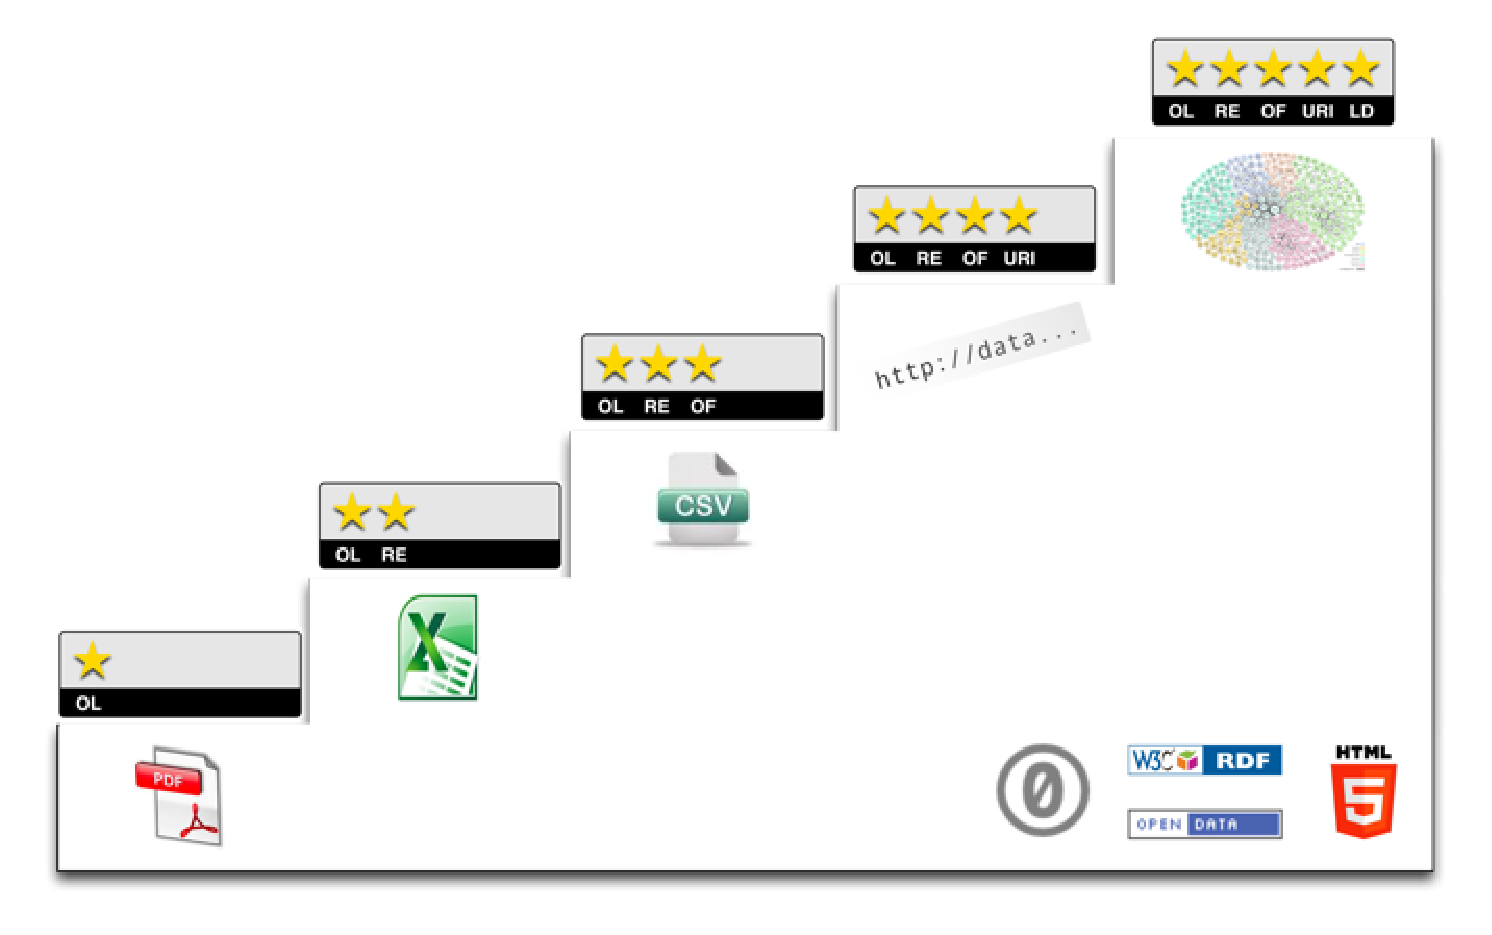
\includegraphics[width=\textwidth]{img/5star_steps.eps}}
\caption{Stupně otevřenosti dat}
\label{obr:5star_steps}
\end{figure}

\newpage

\section{Propojitelná data (Linked Data)}

Linked Data vychází z myšlenky webu aplikované na data. Webu rozumíme jako síti propojených webových stránek. Cílem Linked Data je mít síť propojených, strojově čitelných dat, resp. stavební kámen sémantického webu\cite{sw}. Jedná se v podstatě o další krok v evolučním vývoji webu jako takového.

Podle \cite{linkedData} definujeme základní principy Linked Data jako:

\begin{enumerate}
\item Každá entita je identifikována pomocí HTTP URI    
\item HTTP URI by mělo být vyhledatelné v síti WWW a umožňovat k němu přistupovat a odkazovat se na něj
\item Po přistoupení na HTTP URI entity mají být poskytnuty relevantní informace o dané entitě ve standardizovaném formátu či prostřednictvím API\footnote{Pro popis Linked Data se typicky používá jazyk RDF\cite{RdfConcepts}, k dotazování k datovému API - SPARQL\cite{Sparql}}
\item Data k entitám rozšířit o HTTP URI odkazy na další související entity\footnote{To nám zaručí, že můžeme procházet jednotlivé entity podobným způsobem jako webové stránky v rámci sítě WWW.}
\end{enumerate}

Jak je vidět, Linked Data naplňují všechny požadavky na 5$\bigstar$ kvalitu dat s jednou výjimkou. Linked Data nemusejí být z podstaty otevřenými daty. Určitě si dovedeme představit mnoho scénářů, kdy je přínosem mít propojená, ale privátní data. Typickým příkladem můžou být korporátní intranetové informační systémy.

\section{Otevřená a propojitelná data (Linked Open Data - LOD)}

Otevřená data na úrovni 5$\bigstar$ kvality můžeme tedy chápat jako Linked Open Data. Taková data se mohou stát součástí globálního prostoru sdílených, propojených dat. Připojením datové sady tak můžeme čerpat informační potenciál celého prostoru\footnote{Tvůrci grafu procházejí web a do cloudu přidávají dostupné datasety splňující podmínky Linked Data a podmínky na počet trojic a odkazů. Nezkoumají ale licence jednotlivých datasetů. Některé datesety proto mohou být chráněny specifickými právy.}.

Takový prostor s časem neustále roste. Využití lze nalézt ve většině oblastí lidského konání. Od sdílení a obohacování vědeckých dat, např. biologických, chemických struktur a reakcí s cílem objevů nových postupů v medicíně, přes zpracování dat jednotlivých veřejných správ za účelem kvalitnější veřejné služby až po obohacování kontextu nejrůznějšího mediálního obsahu. 

Na obr. \ref{obr:lodcloud} vidíme příklad vizualizace otevřených a propojených (LOD) dat nazývaný Linked Open Data Cloud. Jedná se o datasety obsahující alespoň 1000 trojic (více v kapitole o RDF) a alespoň 50 odkazů na jiná data ve sdíleném prostoru.  

\newpage

\begin{figure}[h]
\centerline{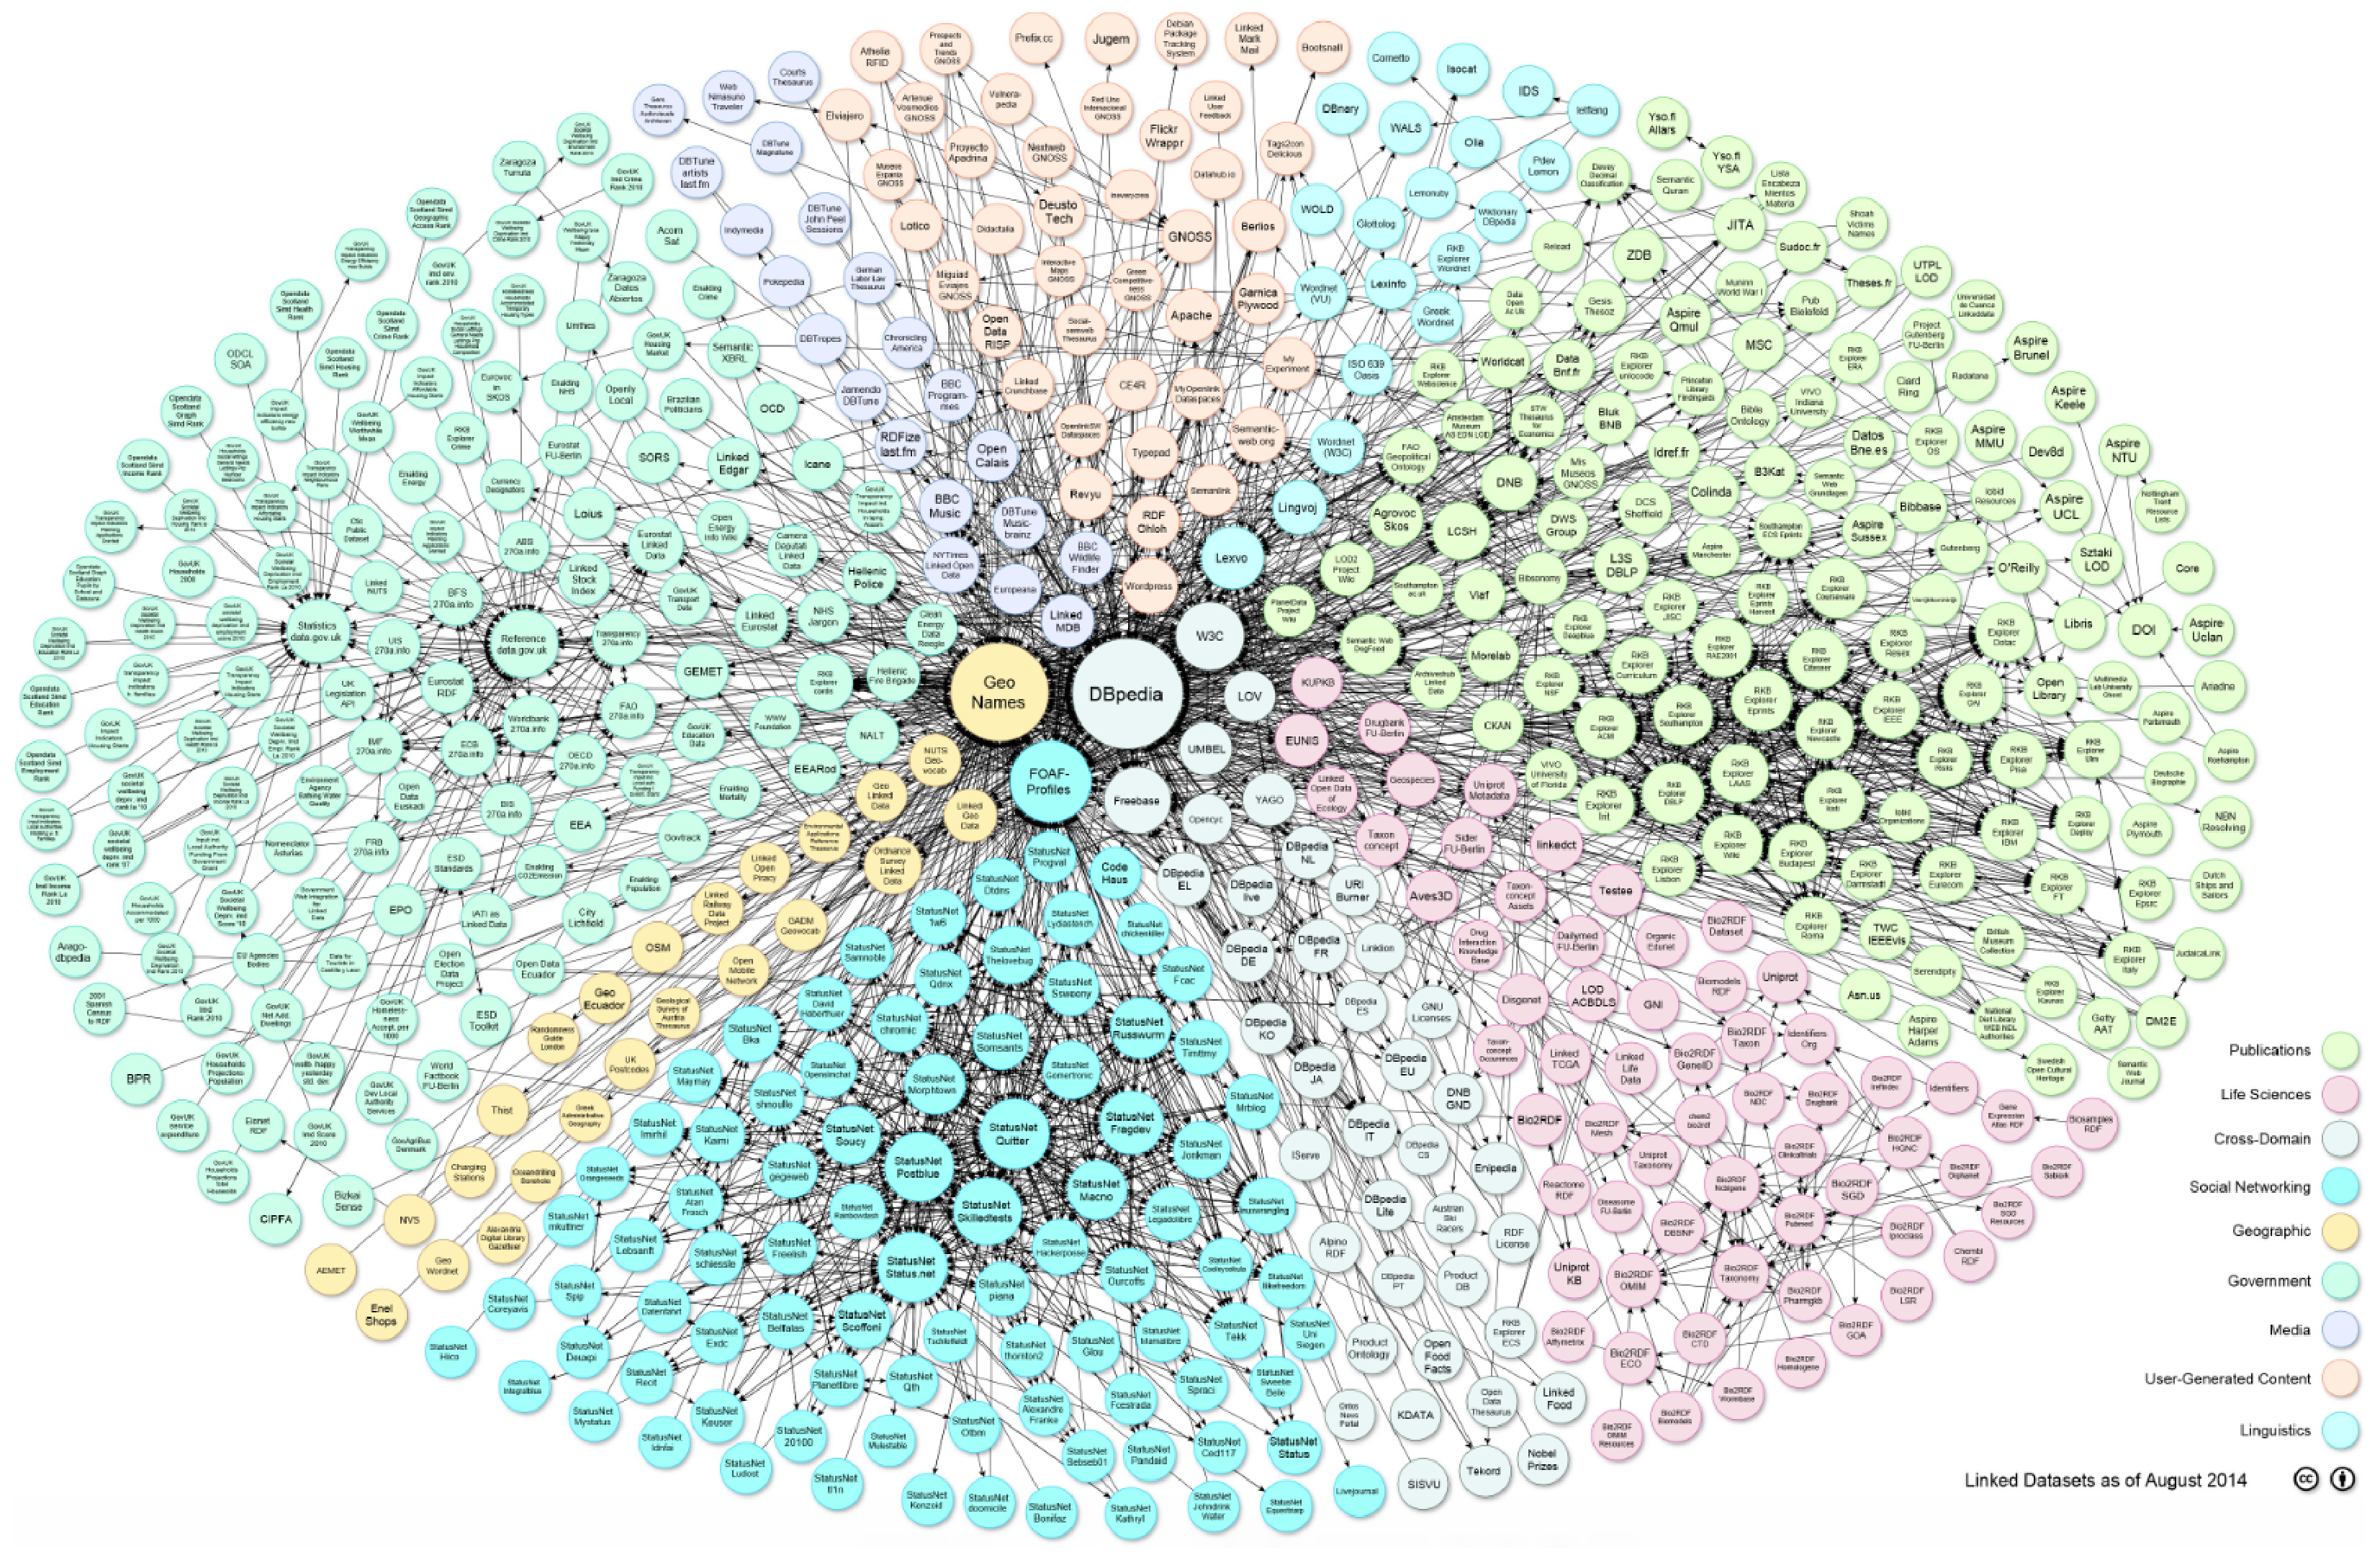
\includegraphics[width=\textwidth]{img/lodcloud.eps}}
\caption{Linked Open Data Cloud, Srpen 2014}
\label{obr:lodcloud}
\end{figure}

\section{Výhody a přínosy otevřených dat a principů Linked data}

\subsection*{Obecné výhody otevřených dat}

\begin{enumerate}
\item Zapojení uživatelů - kontrola, návrhy ke zlepšení dat   
\item Zvýšení transparentnosti vydavatele dat, boj s korupcí
\item Kvalitnější veřejná služba, lepší prezentace subjektu
\item Zvýšení efektivity, úspora nákladů, méně chyb
\item Méně žádostí o data podle zákona č. 106/1999 Sb.\cite{z106} 
\item Široké možnosti dalšího využití - analýzy, statistiky, vizualizace
\end{enumerate}

\subsection*{Výhody principů Linked Data}

\begin{enumerate}
\item Sdílená, rozšiřitelná a snadno znovu použitelná data   
\item Data jsou začleněna do kontextu, resp. lze se odkazovat přímo na data
\item Data jsou propojena s dalšími relevantními daty, informační hodnota dat je tedy tím větší, čím více mají vazeb
\item Standardizované formáty pro publikaci
\end{enumerate}

\newpage

\section{RDF (Resource Description Framework)}
\label{sec:RDF}

Formát RDF byl vyvinut za účelem snadného strojového zpracování a propojování dat. Jedná se o čistě abstraktní formát udávající, jak data popisovat. Nezabývá se tedy konkrétní podobou výsledných dat. 

Základním stavebním kamenem RDF je tvrzení, resp. trojice: \textbf{Subjekt - Predikát - Objekt} (viz Obr. \ref{obr:rdf_basic}). Subjektem je míněn zdroj, který popisujeme. Predikát je vlastnost, která o objektu něco tvrdí. Objekt je hodnota dané vlastnosti. Jednotlivé trojice mohou na sebe navazovat a vytvořit tak orientovaný graf.

\begin{figure}[h]
\centerline{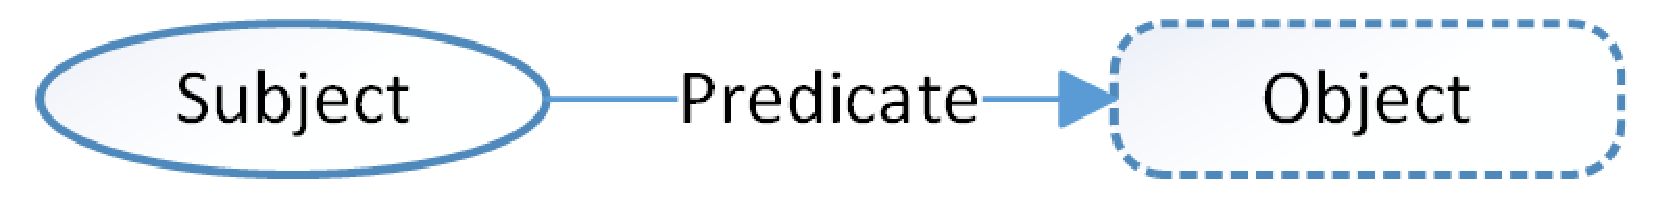
\includegraphics[width=110mm]{img/rdf_basic.eps}}
\caption{Základní RDF trojice}
\label{obr:rdf_basic}
\end{figure}

\subsection*{Nyní definujeme několik pravidel a doporučení pro popisování dat v RDF}

\begin{enumerate}
\item Každý subjekt je jednoznačně identifikován pomocí URI, nebo je označen jako anonymní\footnote{Subjekty, příp. objekty lze označit jako anonymní, resp. pomocí tzv. Blank node. Na anonymní subjekty, resp. objekty ale nelze přímo přistupovat. Používají se typicky k zapouzdření, či jako kontejnery jiných objektů.} 
\item Objektem je buď hodnota (literál), odkaz na subjekt (resource), nebo je označen jako anonymní
\item Pro každý subjekt je specifikován jeho typ (třída) formou URI
\item Každému predikátu je přiřazen také jeho typ formou URI
\item Jednotlivé URI z bodů 3, 4 by měly odkazovat na konkrétní slovníky tříd a predikátů, resp. ontologie
\end{enumerate}

Na obr. \ref{obr:rdf_graph} vidíme příklad jednoduchého grafu ve formátu RDF (aplikována pravidla 1 a 2). Popisuje 3 subjekty a přiřazuje jim konkrétní vlastnosti. Vidíme, že každý subjekt je identifikován vlastním URI. Díky tomu mohou subjekty na sebe odkazovat. Jednotlivé trojice by pak vypadaly takto:

\begin{enumerate}
\item \textit{http://rsmluv.cz/contract/42/1 - Název - Softwarová zakázka}   
\item \textit{http://rsmluv.cz/contract/42/1 - Smluví strana - rsmluv.cz/party/420}
\item \textit{http://rsmluv.cz/party/420 - Název - Magistrát HMP}
\item \textit{http://rsmluv.cz/party/420 - Adresa - rsmluv.cz/party/420/address}
\item \textit{http://rsmluv.cz/party/420/address - Ulice - Staroměstké nám. 4}
\end{enumerate}

\begin{figure}[h]
\centerline{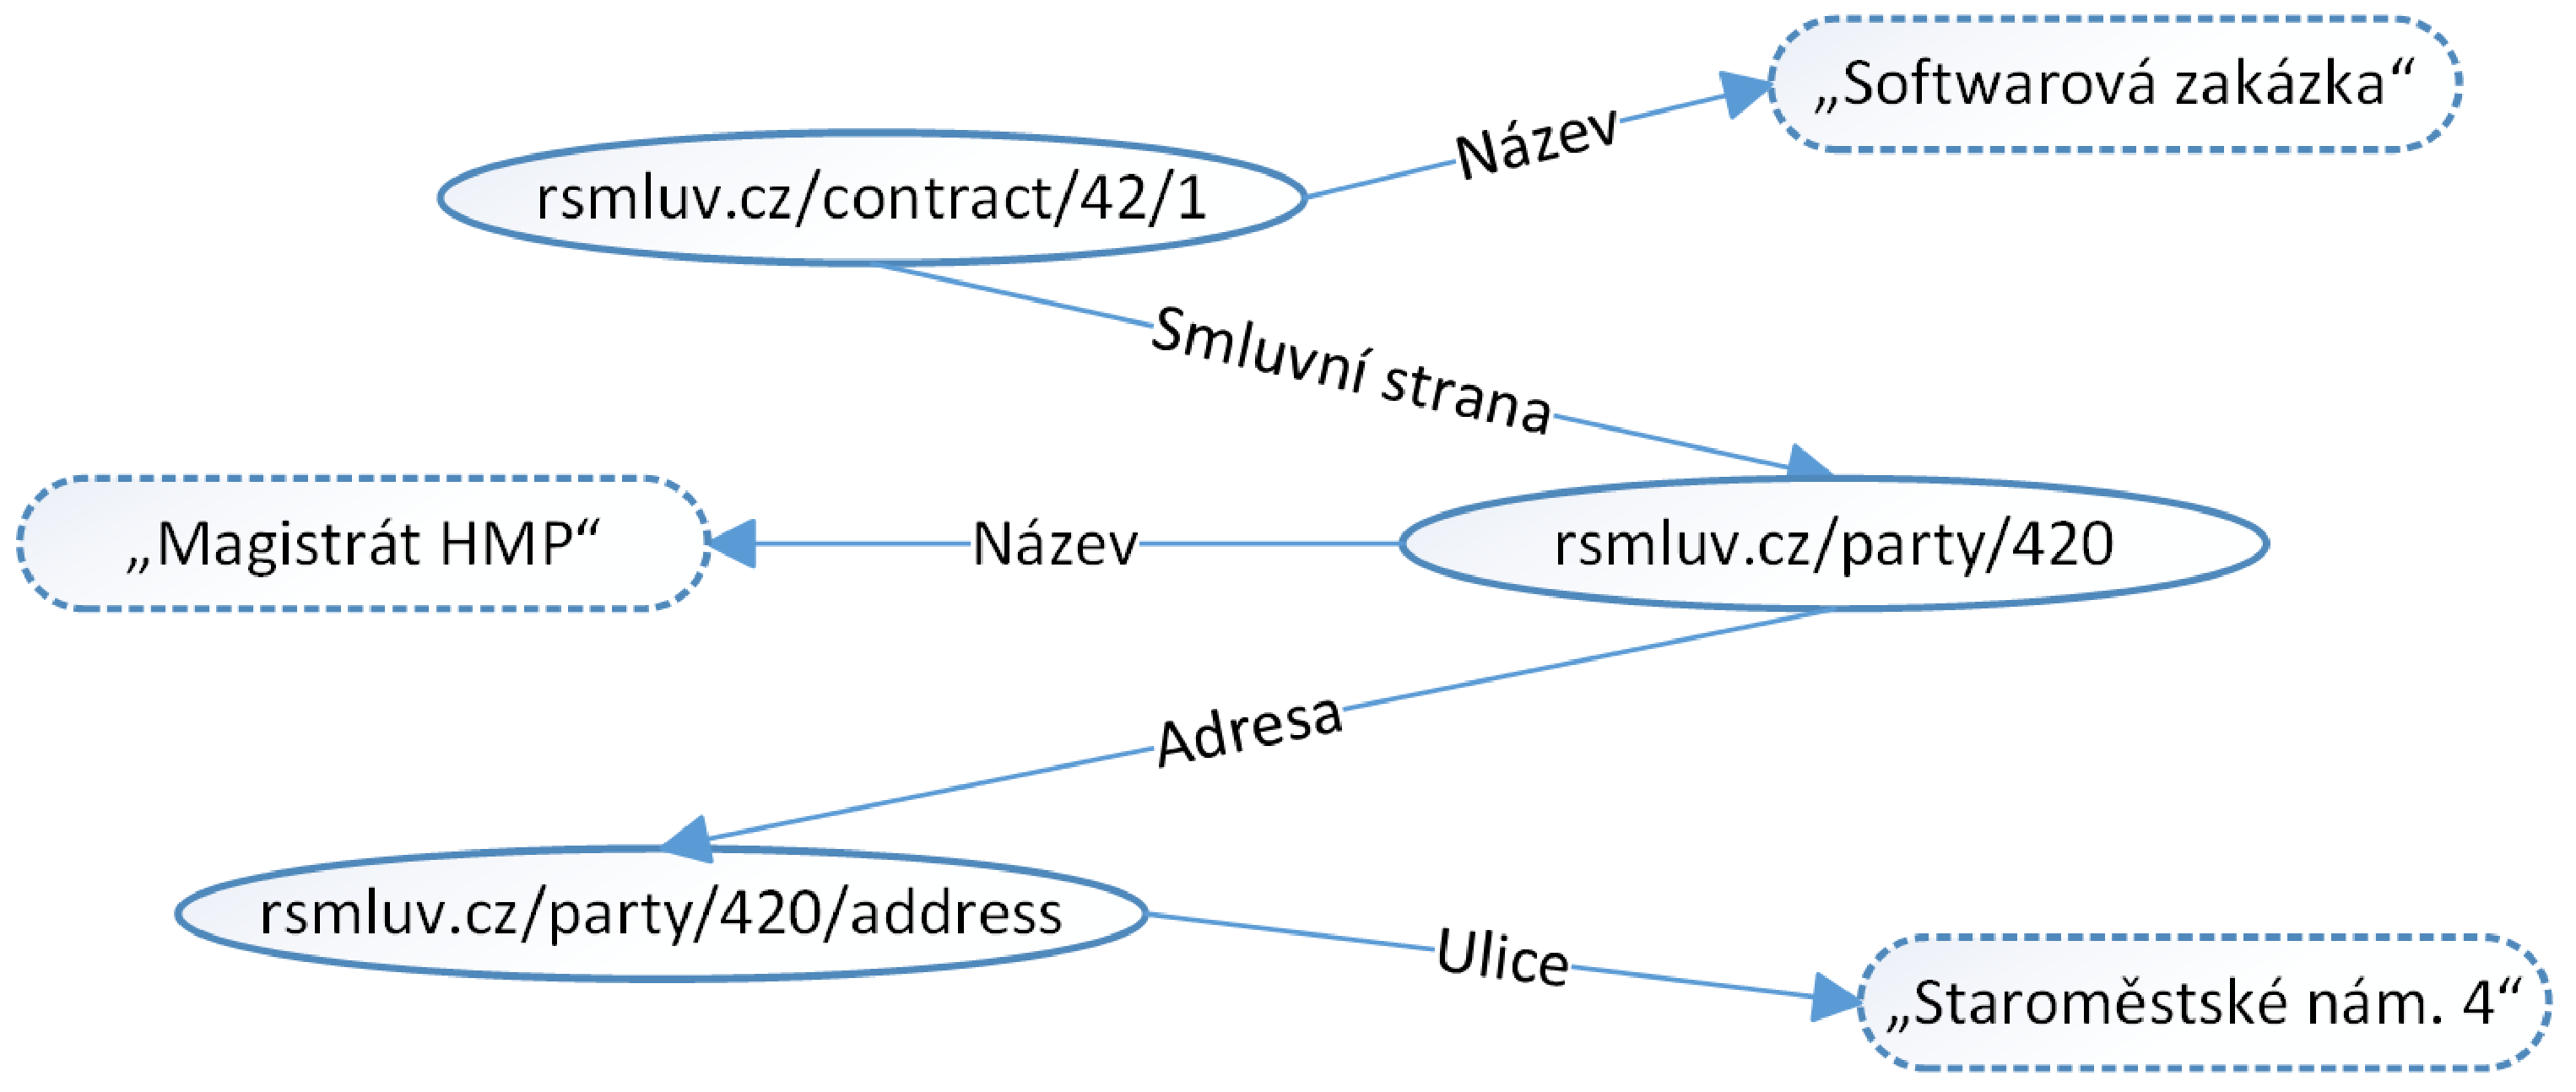
\includegraphics[width=\textwidth]{img/rdf_graph.eps}}
\caption{Jednoduchý RDF graf}
\label{obr:rdf_graph}
\end{figure}

Ze zmíněného příkladu ale není zřejmý význam, resp. sémantika jednotlivých subjektů a predikátů. Je tedy důležité jim přiřadit konkrétní typy. Každý typ by měl být popsaný v konkrétním slovníku tříd a predikátů. Takovéto slovníky nazýváme ontologiemi. Na obr. \ref{obr:rdf_graphWithOntology} vidíme zmíněný příklad rozšířený o přiřazené typy (aplikována pravidla 3, 4, 5)\footnote{Pro zapisování typů se kvůli úspornosti používají prefixy definované typicky na začátku dokumentu.}.

\begin{figure}[h]
\centerline{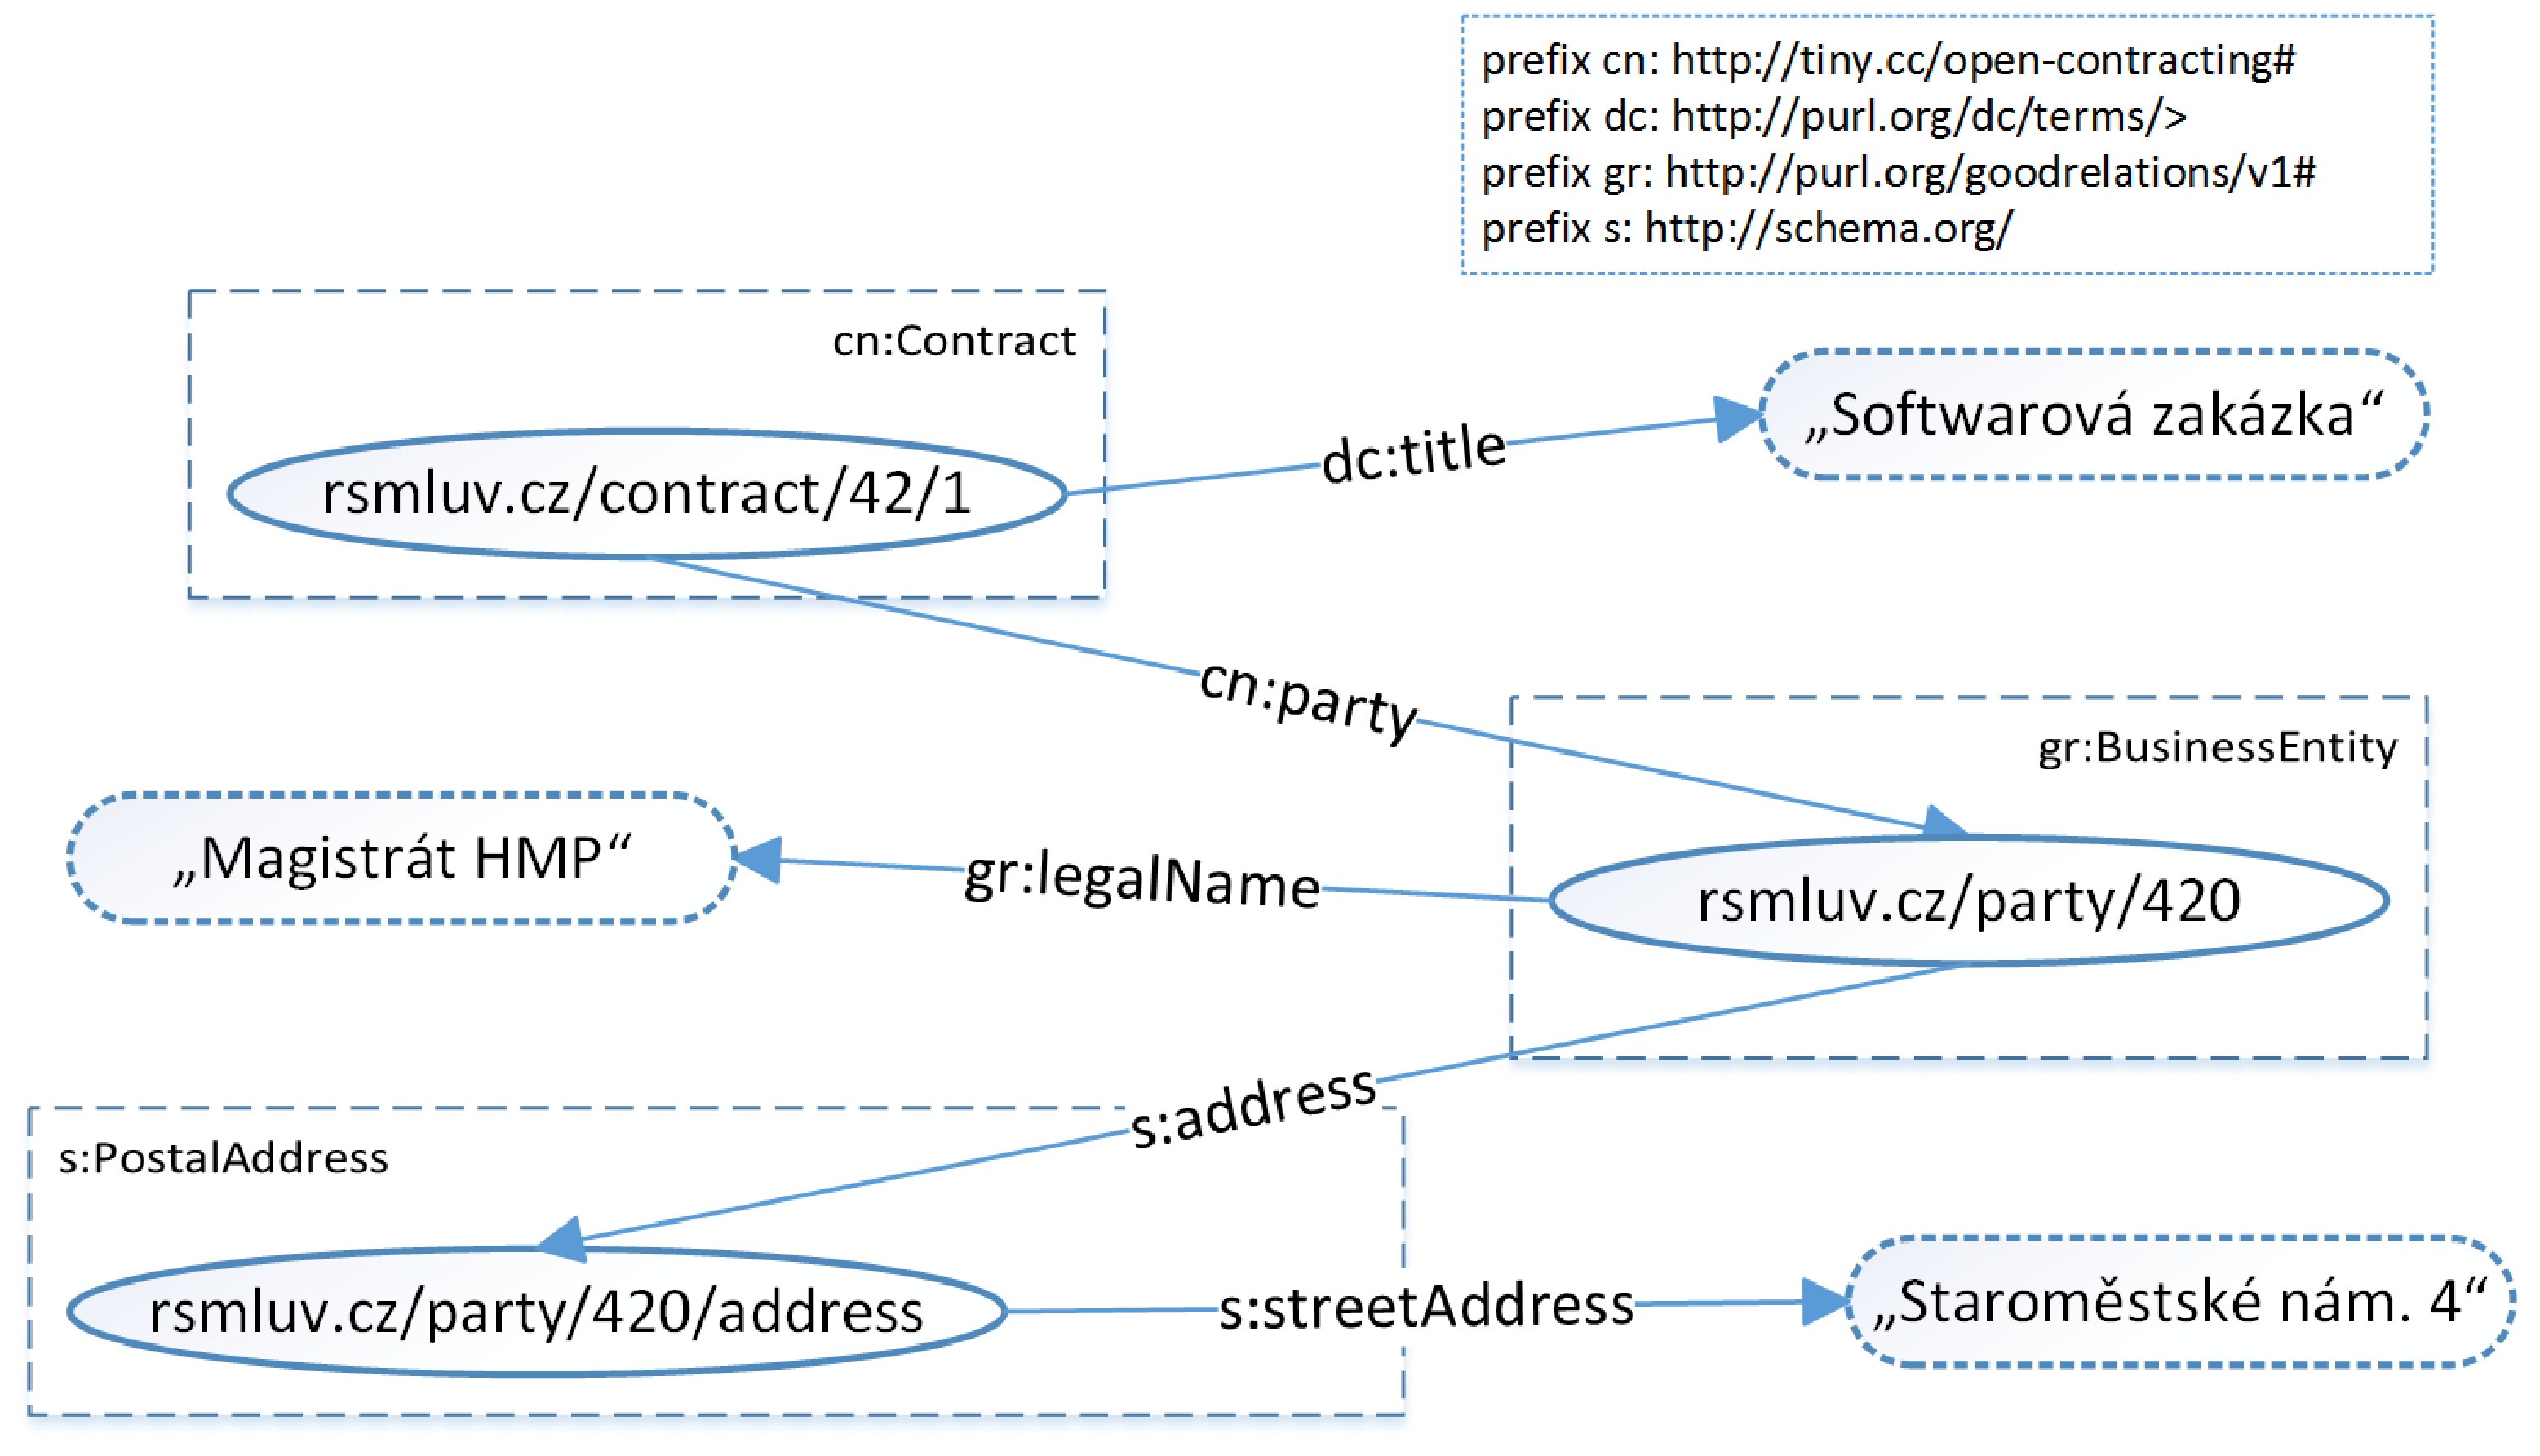
\includegraphics[width=\textwidth]{img/rdf_graphWithOntology.eps}}
\caption{RDF graf s přiřazenými typy}
\label{obr:rdf_graphWithOntology}
\end{figure}

\newpage

\section{RDF Ontologie}

Pod pojmem ontologie si můžeme představit sadu termínů popisujících určitou věcnou oblast. V případě popisování RDF dat definujeme slovník tříd a vlastností (predikátů), které mohou uživatelé ve svých datech používat.

Konkrétní ontologii nelze chápat jako striktně vyžadovaný standard, ale spíše jako sadu doporučení. Buď využijeme k popisu dat nějakou z řady již existujících ontologií, nebo můžeme vytvořit ontologii vlastní. Přesto ale chceme, aby se již existující ontologie používaly co nejvíce. Přínosem je hlavně to, že aplikace a nástroje implementované nad známými ontologiemi budou schopné automaticky rozpoznat naše data\footnote{Mezi všeobecně známé ontologie patří např. DublinCore\cite{dc}, Friend-of-a-Friend\cite{foaf} nebo Schema\cite{schema}. Existuje také katalog ontologií\cite{lov}}. 

Základními jazyky pro modelování RDF dat jsou Web Ontology Language (OWL)\cite{OWL} a RDF Schema (RDFS)\cite{RdfSchema}. Konkrétní specifikace se provádí opět ve formátu RDF a je publikována pod vlastním URI.

Mezi základní výrazové prostředky jazyka OWL a RDFS patří:

\begin{itemize}
\item \textit{owl:Class} - typ entity třída
\item \textit{owl:ObjectProperty} - typ entity vlastnost
\item \textit{owl:FunctionalProperty} - typ jedinečná vlastnost (nemůže se opakovat)
\item \textit{owl:unionOf} - jeden typ třídy z výčtu musí být vyplněn 
\item \textit{owl:equivalentClass} - definuje, že se jedná o třídu odpovídající jiné třídě
\item \textit{owl:equivalentProperty} - definuje, že se jedná o vlastnost odpovídající jiné vlastnosti
\item \textit{rdfs:label} - popis třídy/vlastnosti
\item \textit{rdfs:comment} - komentář třídy/vlastnosti
\item \textit{rdfs:domain} - požadovaný  typ domény třídy/vlastnosti
\item \textit{rdfs:range} - požadovaný rozsah typů třídy/vlastnosti
\item \textit{rdfs:isDefinedBy} - definice zdroje třídy/vlastnosti
\item \textit{rdfs:subClassOf} - definice, že se jedná o podtřídu určité třídy  
\item \textit{rdfs:subPropertyOf} - definice, že se jedná o podvlastnost určité vlastnosti  
\end{itemize}

Na obr. \ref{obr:rdf_ontologyClass} vidíme příklad ontologie třídy Contract. Ontologie nám říká, že se jedná o třídu (typ owl:Class) s názvem Smlouva (rdfs:label), která je podtřídou (rdfs:subClassOf) třídy Document a je definovaná (rdfs:isDefinedBy) v ontologii http://tiny.cc/open-contracting. Kdokoli pak bude zpracovávat entitu označenou tímto typem, tak díky přiřazené ontologii bude schopen určit, že se jedná o smlouvu.

\begin{figure}[h]
\centerline{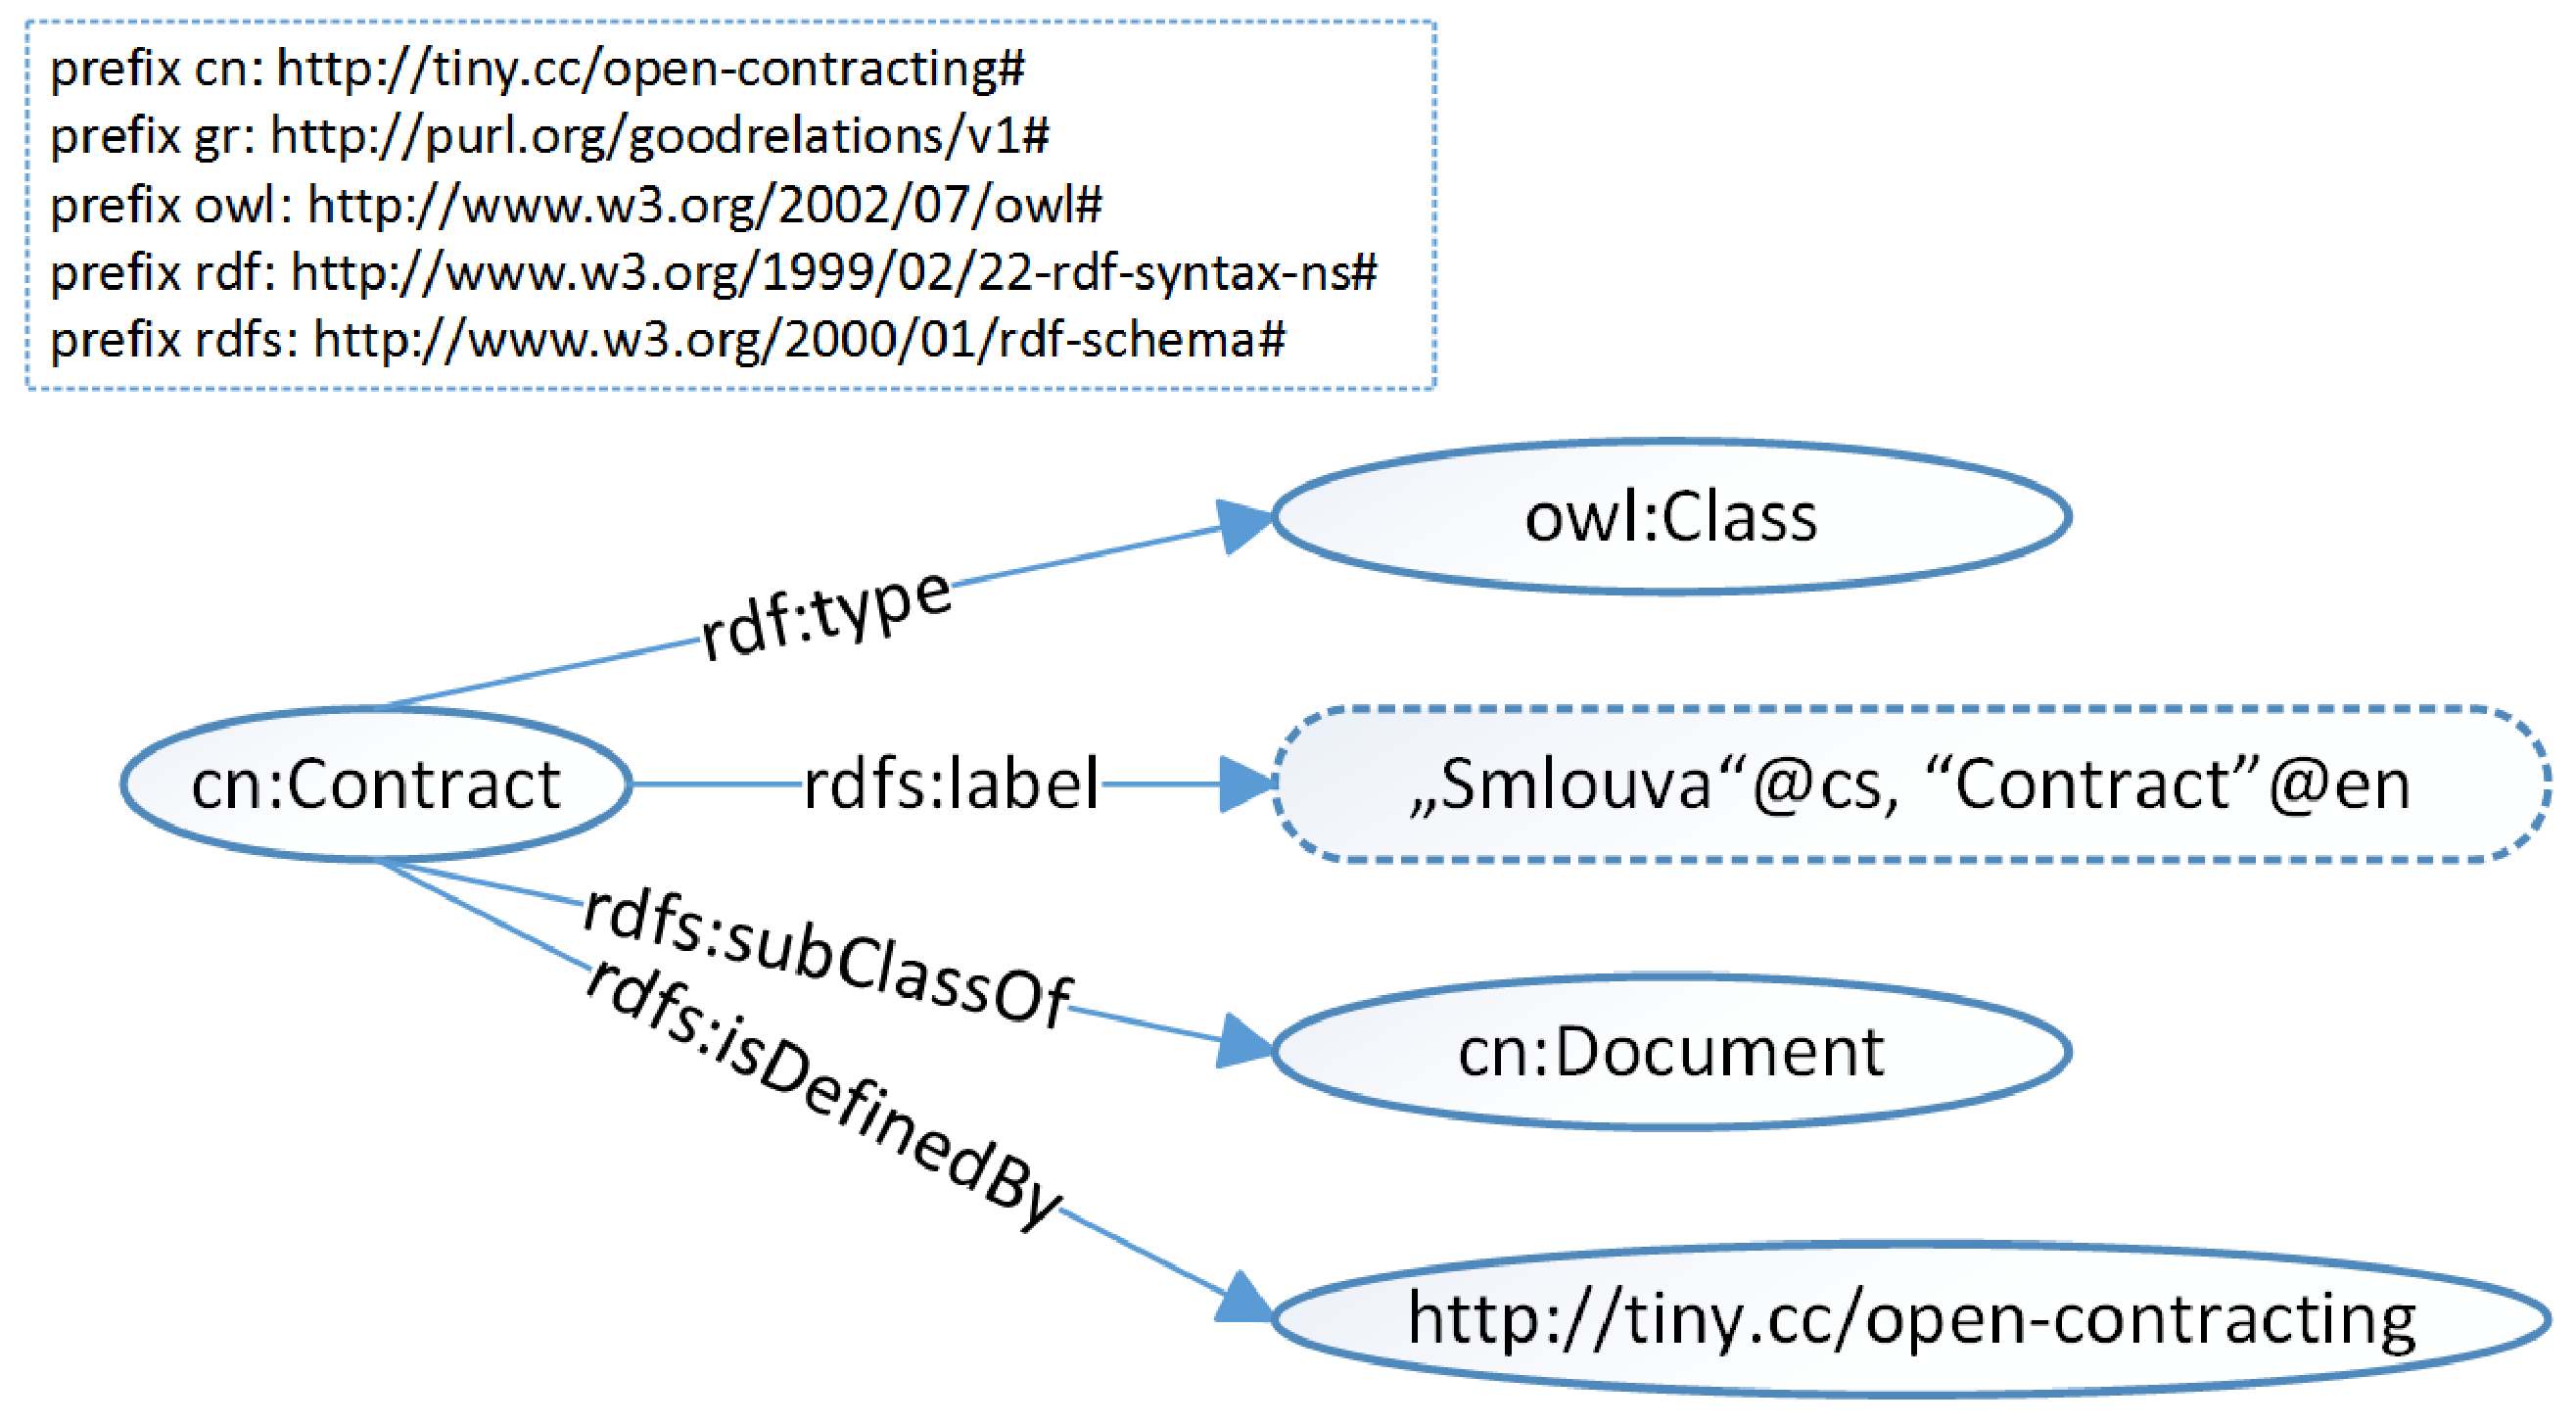
\includegraphics[width=\textwidth]{img/rdf_ontologyClass.eps}}
\caption{Ontologie třídy \textit{Contract}}
\label{obr:rdf_ontologyClass}
\end{figure}

\subsection{Propojování se souvisejícími entitami}

Díky RDF můžeme data reprezentovat jako orientovaný graf. Otázka tedy zní, zdali lze propojovat grafy mezi sebou. Ve formátu RDF je to velmi jednoduché. Jako objekt predikátu stačí položit subjekt z jiného grafu. Díky URI identifikaci entit tedy není rozdílem, zdali je cílovým subjektem entita v lokálních datech, nebo entita cizí.  

V rámci propojování dat s jinými datasety však není neobvyklé, že stejné entity jsou reprezentované v různých datasetech pod vlastními URI. Je tedy třeba vyjádřit, že se jedná o data reprezentující stejné entity. V jazyku OWL za tímto účelem existuje predikát sameAs, kterým můžeme definovat odpovídající si entity (viz Obr. \ref{obr:rdf_ontologyLinks}).

\begin{figure}[h]
\centerline{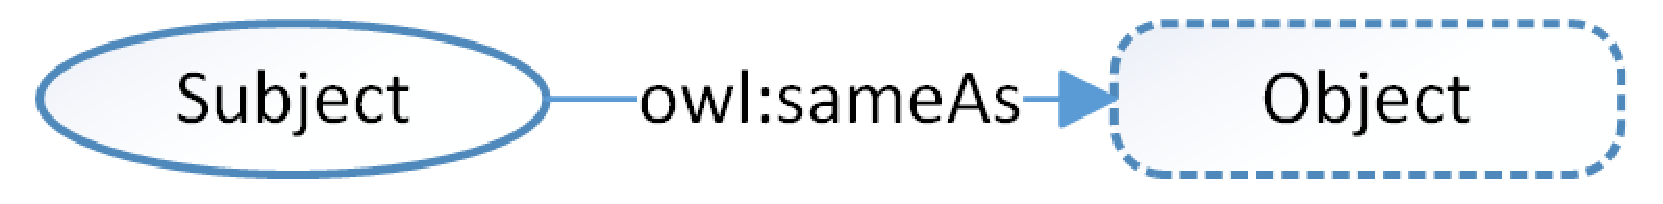
\includegraphics[width=110mm]{img/rdf_ontologyLinks.eps}}
\caption{Odpovídající si entity}
\label{obr:rdf_ontologyLinks}
\end{figure}

\newpage

\section{Publikace}

V minulých kapitolách bylo řečeno, jak popisovat data pomocí RDF. Jednalo se o sémantický popis. Pokud však data chceme publikovat, je třeba konkrétního datového formátu, který definuje syntaxi, resp. jak RDF data serializovat. Takových formátů existuje celá řada, např.:

\begin{itemize}
\item \textbf{N-Triples\cite{N-Triples}} - nejjednodušší serializace RDF grafu v podobě výčtu trojic
\item \textbf{N-Quads\cite{N-Quads}} - rozšíření pro N-Triples s možností zaznamenat více grafů
\item \textbf{RDF/XML\cite{RDF/XML}} - RDF graf serializovaný do XML, využívající prefixového zápisu
\item \textbf{Turtle\cite{Turtle}} - úsporný textový formát s možností komprese trojic, využívající prefixových zápisů
\item \textbf{Trig\cite{Trig}} - rozšíření Turtle pro použití nad více grafy
\item \textbf{RDFa\cite{RDFa}} - serializace RDF do (X)HTML dokumentů, využívající prefixového zápisu
\item \textbf{JSON-LD\cite{JSON-LD}} - specifický zápis RDF grafu, využívající mapování položek JSON dokumentu na RDF ontologie
\end{itemize}

Pro potřeby této práce si vystačíme s formáty N-Triples, Turtle a JSON-LD. Vysvětlíme si je na příkladech. Jako data k serializaci použijeme příklad z obr. \ref{obr:rdf_graphWithOntology}.

\subsection{Příklad dat serializovaných ve formátu N-Triples}

Serializace RDF dat do N-Triples je velmi jednoduchá. Jedná se o seznam trojic oddělených tečkou. Každá trojice je uvedena na vlastním řádku. Tento formát nepoužívá prefixové zkracování URI. Je vhodný pro proudové zpracování velkého množství dat (viz Obr \ref{lst:ntriples_example})\footnote{Trojice nejsou z důvodu přehlednosti uvedeny na samostatných řádcích}.\\

\lstinputlisting[label=lst:ntriples_example,caption=Příklad RDF dat - N-Triples, language=XML]{code/ntriples_example.nt}

\subsection{Příklad dat serializovaných ve formátu Turtle}

Formát Turtle umožňuje zkracování URI pomocí prefixů. Umožňuje také zkracovat zápis tím, že nemusíme zapisovat opakující se subjekt. Jednotlivé dvojice predikát-hodnota lze tak přehledně mít u jednoho subjektu. Oddělovačem mezi dvojicemi v rámci subjektu je středník, blok informací o daném subjektu je zakončený tečkou. Pro definování typu subjektu se může použít klíčové slovo \uv{a}, namísto predikátu rdf:type. Výhodou formátu je úspornost a velmi dobrá lidská čitelnost (viz Kód \ref{lst:turtle_example}).\\

\lstinputlisting[label=lst:turtle_example, caption=Příklad RDF dat - Turtle, language=XML]{code/turtle_example.ttl}

Díky dobré čitelnosti, se formát Turtle hojně používá pro zapisování ontologií. V kódu \ref{lst:turtleOntology_example} vidíme znázorněnou jednoduchou ontologii. Popisuje 2 objekty. Prvním je třída Contract (typ owl:Class). Definuje, že se jedná o smlouvu, je podtřídou (rdfs:subClassOf) třídy Document a je definována v ontologii (rdfs:DefinedBy) http://tiny.cc/open-contracting. Je to serializovaný zápis ontologie z obr. \ref{obr:rdf_ontologyClass}. Druhým objektem je vlastnost party (typ owl:ObjectProperty). V predikátu rdfs:domain je specifikováno, že vlastnost party může být použita u třech tříd, a to Contract, Order nebo Invoice. Predikát rdfs:range znamená, že očekávaný přiřazený objekt je typu gr:BusinessEntity.\\

\lstinputlisting[label=lst:turtleOntology_example, caption=Příklad RDF Ontologie - Turtle, language=XML]{code/turtleOntology_example.ttl}

\subsection{Příklad dat serializovaných ve formátu JSON-LD}

JSON-LD je jedním z poměrně nových formátů pro serializaci RDF. Jednou z motivací k vzniku byla snaha využít hojně využívané JSON dokumenty v dnešních aplikacích a co možná nejefektivněji z nich vytvořit RDF data.

Uveďme si modelový příklad. V kódu \ref{lst:json_example} jsou ne-RDF data ve formátu JSON. Jsou validní vůči nějakému JSON Schématu a používají se v konkrétních aplikacích.  

V kódu \ref{lst:jsonld_example} máme stejná data v RDF podobě. Jak je vidět, jednotlivým objektům je přiřazen typ a URI. Použije se k tomu klíčových slov @type, resp. @id. K dokumentu je také přiložen kontext (klíčové slovo @context), kde se definuje mapování vlastností původního JSON dokumentu na RDF ontologie. Zachovává se tedy původní struktura JSON dokumentu. Kontext však nemusí být přímo součástí JSON-LD dokumentu, lze se na něj odkazovat. 

Výsledkem tedy může být JSON-LD soubor (viz Kód \ref{lst:jsonldWithContext_example}). Jedná se tedy pouze o lehce rozšířený původní JSON dokument. Z tohoto důvodu bude pravděpodobně takový dokument nadále validní vůči JSON Schématu a použitelný ve stávajících aplikacích. Přináší však tu výhodu, že se zároveň jedná o RDF data.

\newpage

\lstinputlisting[label=lst:json_example, caption=Obyčejný JSON dokument, language=XML]{code/json_example.json}

\lstinputlisting[label=lst:jsonld_example, caption=Příklad RDF dat - JSON-LD, language=XML]{code/jsonld_example.jsonld}

\lstinputlisting[label=lst:jsonldWithContext_example, caption=Příklad RDF dat - JSON-LD s Contextem, language=XML]{code/jsonldWithContext_example.jsonld}
\chapter{Otevřené smlouvy}
\label{sec:kap3}

\section{Situace ve veřejné správě ČR}

Pokud se veřejná instituce rozhodne pro publikaci údajů o smlouvách, má dnes (rok 2015) v podstatě dvě možnosti. První možností je vyvinutí vlastní iniciativy a zveřejnění smluv na svých webových stránkách. Druhou variantou je využití již existujícího registru smluv na portálu veřejné správy\cite{portalgov}. Registr je to značně minimalistický, ale řešení je to dostačující.

Vzhledem k chystanému zákonu o registru smluv se ale budoucnost stávajícího registru jeví jako značně nejistá. Lze totiž očekávat, že s velkou pravděpodobností vznikne registr zbrusu nový\footnote{Zákon o Registru smluv - tisk 42\cite{z42} byl definitivně schválen 24.11.2015 poslaneckou sněmovnou. Neprošel však ještě celým legislativním procesem. Je už ale téměř jisté, že opravdu vznikne nový registr smluv.}.

První otázkou je, kolik veřejných institucí již smlouvy zveřejňuje. Na portálu veřejné správy lze dohledat řádově několik desítek subjektů. O těchto institucích můžeme prohlásit, že oficiálně zveřejňují smlouvy. Informace o subjektech, které zveřejňují na svých webových stránkách, není systematicky zdokumentovaná vůbec. Lze ale očekávat, vzhledem k celkovému množství veřejných institucí a počtu subjetků zveřejňujících na portálu veřejné správy, že se jedná o nepatrný zlomek. Klíčem ke zlepšení situace by mohl být již zmíněný zákon o registru smluv, který mimo jiné ukládá povinnost, že pokud smlouva není zveřejněná na internetu, tak je neplatná.

Další otázkou je, jak mají data o zveřejněných smlouvách vypadat, které položky musí, či nemusí obsahovat. Není přeci cílem, aby každá veřejná instituce zveřejňovala smlouvy jinak. Obecně chybí datový standard a metodika pro zveřejňování smluv. Pokrok v tomto směru udělalo Ministerstvo vnitra ČR, které plánuje vydat sadu standardů pro publikovatelné datové sady veřejných institucí\footnote{Standardy publikace a katalogizace otevřených dat veřejné správy ČR\cite{odgov}}. Bude se mimo jiné jednat o jakési minimální nutné doporučení, co konkrétní datová sada musí obsahovat.

V úvodu již bylo řečeno, že pod záštitou Oživení o.s.\cite{oz} a EconLabu\cite{econLab} (dříve Centrum aplikované ekonomie o.s.) vzniká datový standard pro otevřené smlouvy. Hlavními postavami koordinujícími vývoj standardu se stali PhDr. Ing. Jiří Skuhrovec a Mgr. Lenka Franková. Na tvorbě standardu participuji a mohu konstatovat, že základní verze je již hotová\footnote{Původní, nerozšířený koncept standardu vyplynuvší z práce akční skupiny je k nalezení na webu iniciativy Bezkorupce\cite{standard}}. Velmi pozitivní zprávou je to, že se tento standard s velkou pravděpodobností dostane do oficiálního doporučení Ministerstva vnitra ČR. Zdá se tedy, že celá tato snaha má smysl.

Standardem pro smlouvy to ale nekončí. Myšlenka úzké spolupráce zástupců měst a obcí, akademické a neziskové sféry se osvědčila. Výsledkem je vznik organizace Otevřená města\cite{otv}, která má za cíl sdružovat veřejné instituce. Pod společnou taktovkou pak financovat společné otevřené projekty. Prvním společným projektem je právě registr smluv.

\section{Standard pro zveřejňování smluv}

V této kapitole se podrobněji seznámíme se standardem pro zveřejňování smluv. Nejdříve je vyložena základní struktura datového standardu, poté jsou popsány konkrétní položky standardu a číselníky. Následně jsou popsány způsoby publikace. Na závěr zmíníme několik informací o vznikající metodice pro zveřejňování smluv. 

\subsection{Základní struktura}

Základním objektem, který slouží k reprezentaci dat, je dokument. Jedná se o abstraktní entitu, která nabývá tří rozšíření typu smlouva/příloha/dodatek. Tato rozšíření obsahují všechny položky obsažené v dokumentu a navíc konkrétní položky pro daný typ.
Smluvní strany jsou separátní objekty navázané buď na smlouvu, objednávku nebo fakturu pomocí jednoznačného identifikátoru.
Objednávka a faktura jsou separátní objekty, které se mohou vázat na konkrétní smlouvu/přílohu/dodatek pomocí jednoznačného identifikátoru.
Rozšiřující entity mohou být součástí smlouvy, příp. objednávky. Reprezentují důležité události v životním cyklu dokumentu a jednotlivé transakce (viz. Obr. \ref{obr:standardDatamodel}). 

\begin{figure}[H]
\centerline{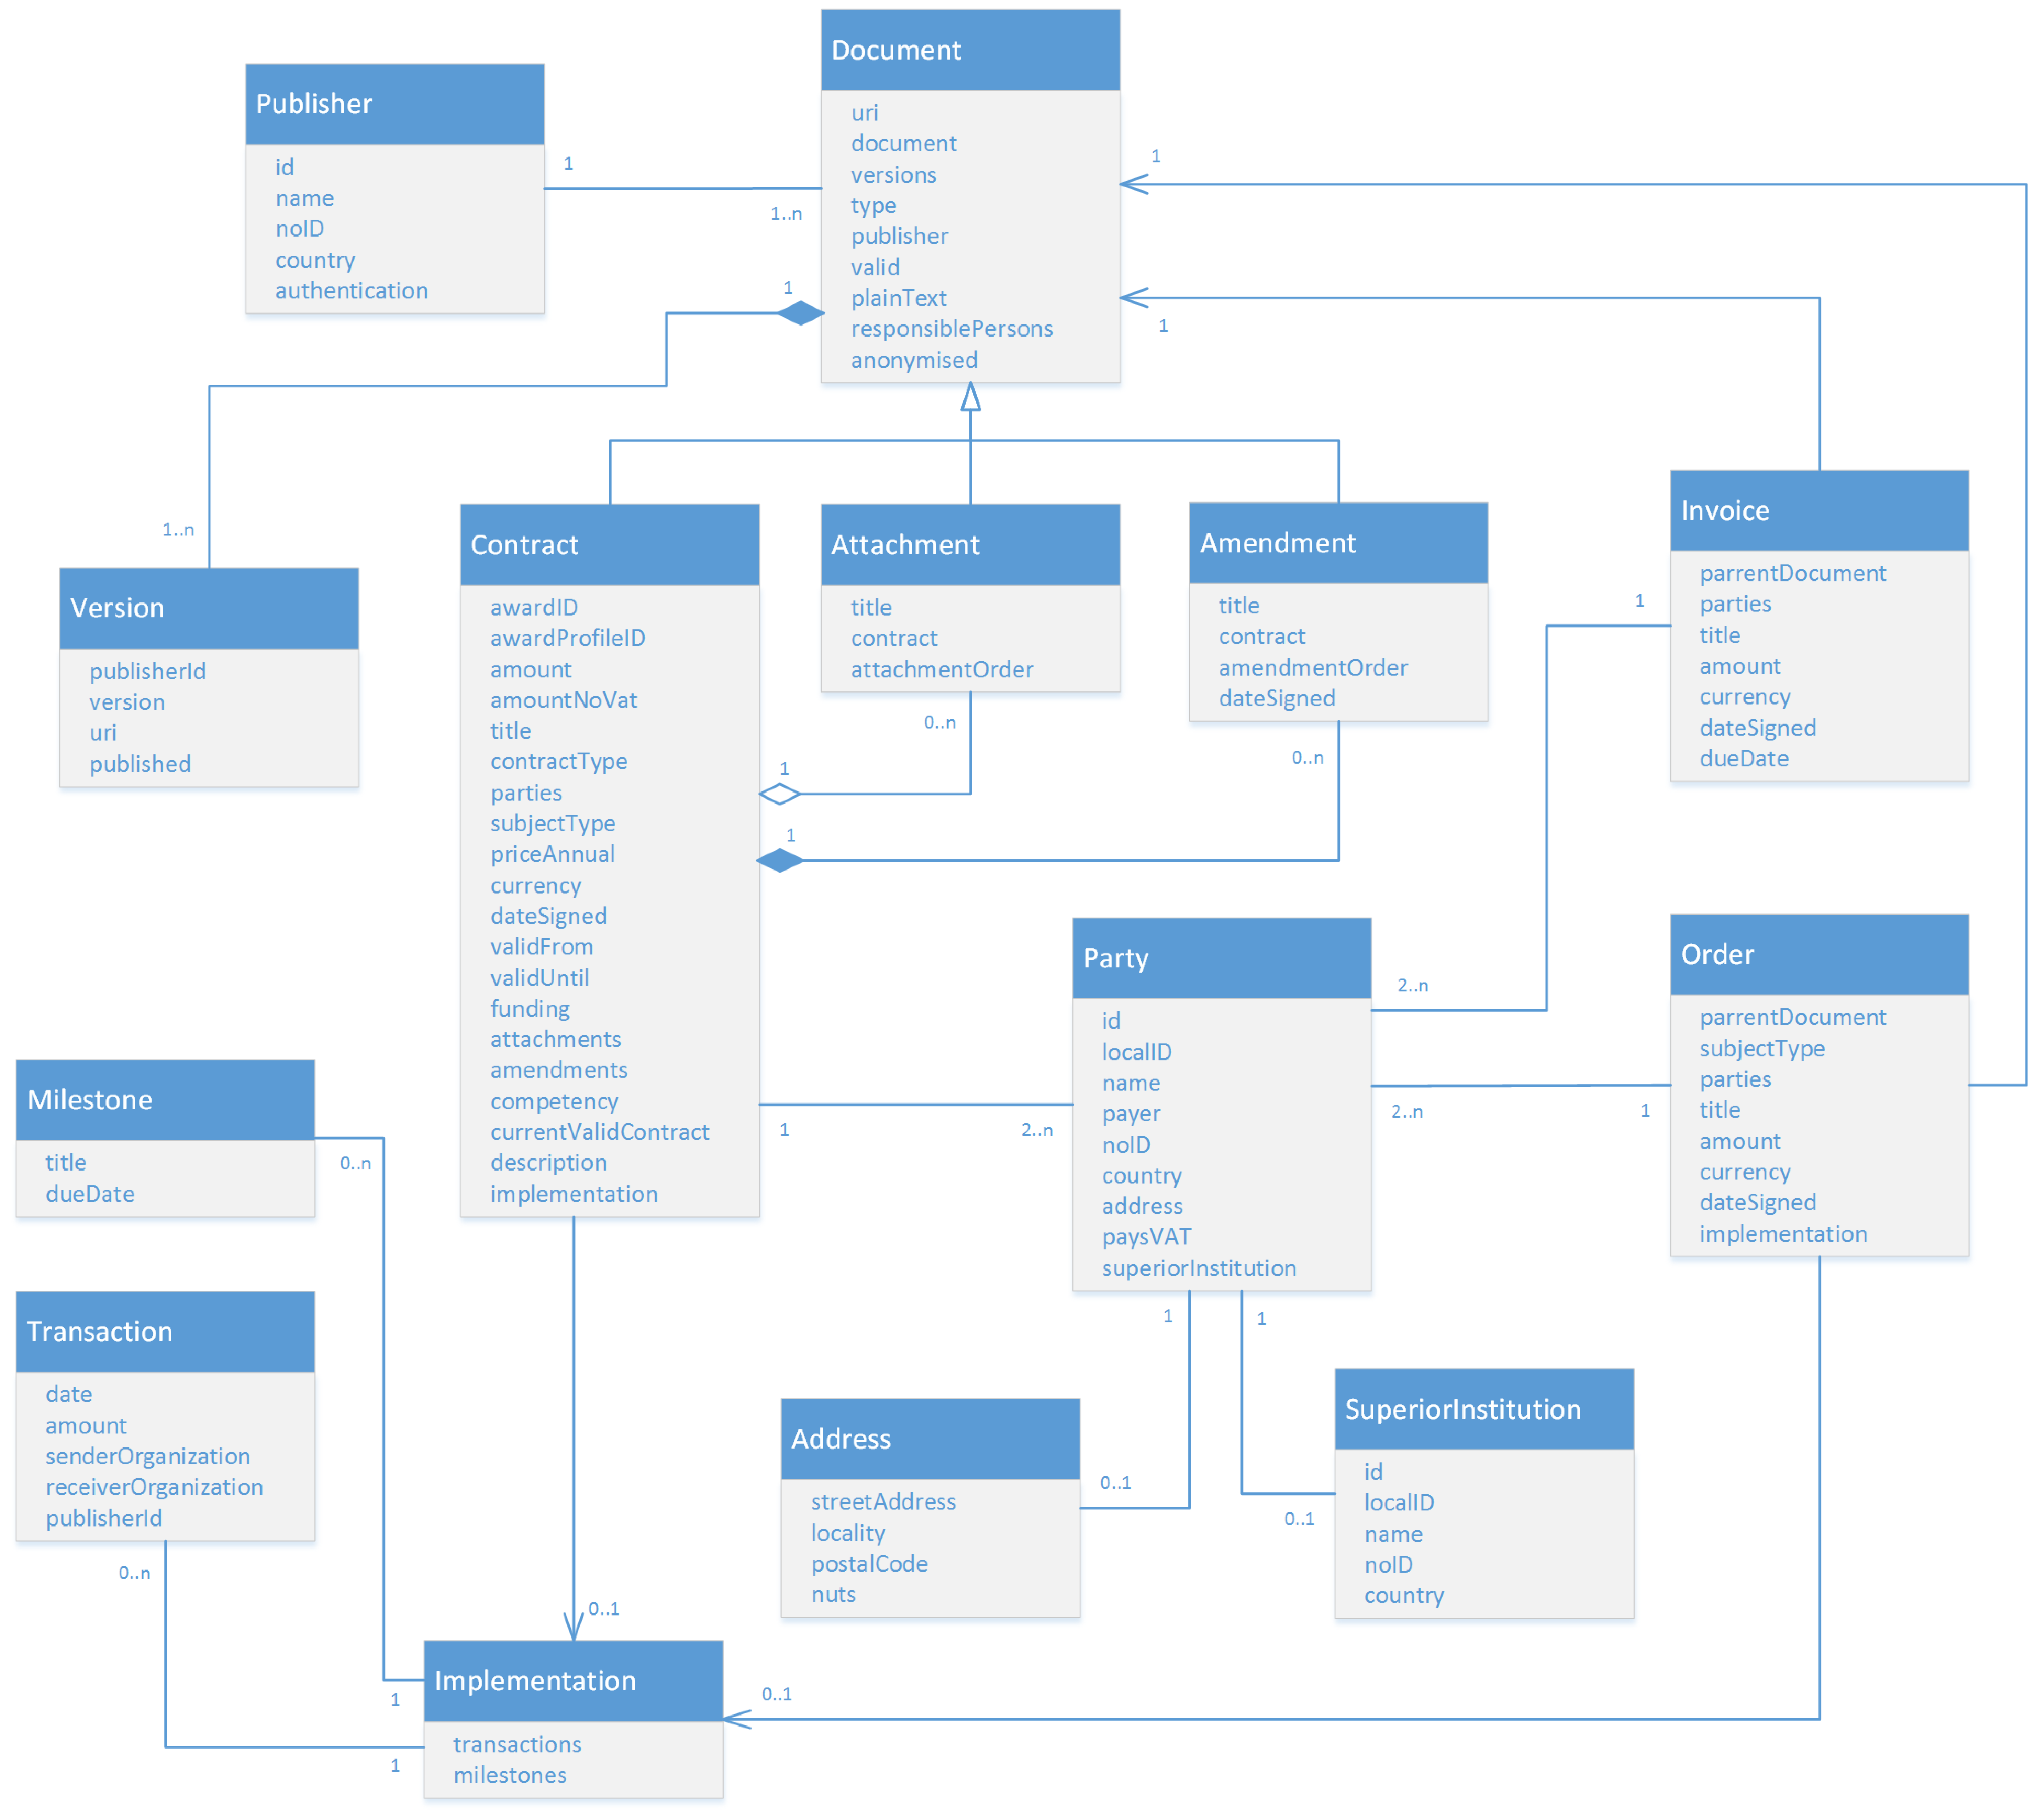
\includegraphics[width=\textwidth]{img/standardDatamodel.eps}}
\caption{Datový standard pro zveřejňování smluv - UML diagram}
\label{obr:standardDatamodel}
\end{figure}

\subsubsection*{Reprezentované entity}

\begin{itemize}
\item \textbf{Dokument} - základní abstraktní struktura pro evidování údajů o smlouvách/přílohách/dodatcích
	\begin{itemize}
    \item \textbf{Smlouva} - detailní popisné údaje smlouvy
    \item \textbf{Příloha} - popisné údaje přílohy 
    \item \textbf{Dodatek} - popisné údaje dodatku
    \item \textbf{Vydavatel} - informace o vydavateli, který zveřejňuje údaje o smlouvách
    \item \textbf{Verze} - identifikace jednotlivé verze dokumentu 
	\end{itemize}
\item \textbf{Smluvní strana} - popisné údaje smluvní strany 
	\begin{itemize}
    \item \textbf{Nadřazená instituce} - informace o řídící nebo ovládající právní osobě vystupující u smluvní strany
    \item \textbf{Adresa} - podrobné údaje o adrese u smluvní strany 
	\end{itemize}
\item \textbf{Objednávka} - popisné údaje objednávky, jedná se o doplňující informace k smlouvě/příloze/dodatku
\item \textbf{Faktura} -  popisné údaje faktury, jedná se o doplňující informace k smlouvě/příloze/dodatku
\item \textbf{Rozšiřující entity} - rozšířené informace ke smlouvě, příp. objednávce
	\begin{itemize}
    \item \textbf{Milník} - reprezentuje důležitou událost v životním cyklu smlouvy
    \item \textbf{Transakce } - reprezentuje proběhlou platbu na základě smlouvy 
	\end{itemize}
\end{itemize}

Datový model je rozdělen do tabulek podle jednotlivých reprezentovaných entit. Každá dílčí položka entity obsahuje tyto informace:

\begin{table}[h]
\centering
\rowcolors{1}{validateB}{validateB}
\begin{tabular}{ll}
\hiderowcolors \textbf{Název pole} & \textbf{Popis} \\ \showrowcolors
\hline
Název pole & Jméno reprezentující danou položku \\
Datový typ & Přípustný datový typ položky \\
Validita & Stupeň kvality položky. \\
Popis & Podrobný popis položky \\
\end{tabular}
\caption{Položky tabulek datového standardu}
\end{table}

U každé zveřejněné smlouvy rozlišujeme tři stupně validity, resp. správnosti a úplnosti dat: A (kvalitní), B (dobrý), C (základní). Dokumenty musí splňovat alespoň minimální přípustnou kvalitu C. Pokud je nějaký atribut požadován pro stupeň validity C, je níže v textu označen např. takto (C). Položky doplněné systémem jsou označeny (S). Nepovinné položky jsou značeny (N), hvězdička znamená, že položka je kontrolována pokročilejším pravidlem popsaném u konkrétní položky. 

\begin{table}[h]
\centering
\begin{tabular}{lcl}
\textbf{Status} & \textbf{Validita} & \textbf{Popis} \\
\hline
Nepovinné & N & Nepovinná položka \\
\rowcolor{validateC}Základní & C & Povinná položka \\
\rowcolor{validateB}Dobrý & B & Rozšiřující položka pro status \uv{Dobrý} \\
\rowcolor{validateA}Kvalitní & A & Rozšiřující položka pro status \uv{Kvalitní} \\
\rowcolor{validateS}Systémové & S & Položka doplněná systémem \\
\end{tabular}
\caption{Validita}
\end{table}

\subsubsection*{Doplňující validační pravidla}

Na entity se vztahují další validační pravidla, která nelze přehledně zachytit v rámci popisu jednotlivých položek. Jejich výčet je zde.

\begin{itemize}
\item Dokument je buď v strojově čitelném formátu (viz. Akceptovatelné soubory), nebo je k němu poskytnut plain text. Pro smlouvy účinné od 1.6.2015\footnote{Předběžné, bude upřesněno} je přípustná pouze varianta ve strojově čitelném formátu.
\item U smlouvy typu darovací nesmí být připojeny faktury, ani jedna smluvní strana nesmí být identifikována jako Payer.
\item Entita (Vydavatel/Smluvní strana/Nadřazená instituce) má vyplněno buď ID, a nebo NoID = \uv{true}.
\end{itemize}

\subsubsection*{Akceptovatelné soubory}

Dokumenty připojené ke smlouvám by měly být strojově čitelné, resp. v těchto formátech:

\begin{table}[h]
\centering
\begin{tabular}{lcl}
\textbf{Formát} & \textbf{Validita} & \textbf{Popis} \\
\hline
\rowcolor{validateC}PDF & C & Portable Document Format - ideálně strojově čitelný \\
\rowcolor{validateC}DOC & C & Textový dokument Microsoft Word \\
\rowcolor{validateC}XLS & C & Tabulka Microsoft Excel \\
\rowcolor{validateB}DOCX & B & Textový dokument Microsoft Word \\
\rowcolor{validateB}ODT & B & Textový dokument OpenDocument \\
\rowcolor{validateB}XLSX & B & Tabulka Microsoft Excel \\
\rowcolor{validateB}ODS & B & Tabulka OpenDocument \\
\end{tabular}
\caption{Akceptovatelné soubory}
\end{table}

\newpage

\subsection{Reprezentované entity}

\medskip

\subsubsection*{Dokument}

\begin{center}
\begin{longtable}{lp{20mm}cp{65mm}}
\label{grid_mlmmh} \\
\multicolumn{1}{l}{\textbf{Název pole}} & 
\multicolumn{1}{l}{\textbf{Datový typ}} & 
\multicolumn{1}{l}{\textbf{Validita}} & 
\multicolumn{1}{l}{\textbf{Popis}} \\ \hline 
\endfirsthead
\multicolumn{1}{l}{\textbf{Název pole}} & 
\multicolumn{1}{l}{\textbf{Datový typ}} & 
\multicolumn{1}{l}{\textbf{Validita}} & 
\multicolumn{1}{l}{\textbf{Popis}} \\ \hline 
\hline
\endhead
\endfoot
\caption{Vlastnosti dokumentu}
\endlastfoot
\rowcolor{validateS}URI & String URI & S & Jednoznačný identifikátor formou URL. Typicky rsmluv.cz/[Typ]/[Id]/[Version], kde Version je vzestupné číslování verzí při změnách dokumentu či metadat \\
\rowcolor{validateS}Document & String URI & S & Adresa URL fyzického umístění dokumentu. Typicky rsmluv.cz/[Typ]/[Id]/[Version]/File, viz akceptovatelné soubory \\
\rowcolor{validateS}Versions & Object array & S & Údaje o verzi dokumentu. Viz entitia Verze \\
\rowcolor{validateC}Type & String/ String enum & C & Typ dokumentu. Nabývá hodnot - Smlouva/Příloha/Dodatek \\
\rowcolor{validateC}Publisher & Reference & C & Informace o vydavateli. Viz entitia Vydavatel \\
\rowcolor{validateB}Valid & Boolean & B/S & Indikuje, zda dokument je platný, tj. nebyl zneplatněn nebo nahrazen novou verzí \\
\rowcolor{validateB}PlainText & String & B/S & Prostý text dokumentu (nestrukturovaný, indexovatelný), alternativa pro scanované dokumenty \\
\rowcolor{validateB}ResponsiblePersons & String array & B & Výčet odpovědných osob \\
\rowcolor{validateB}Anonymised & Boolean & B & Značí, zda-li byla provedena anonymizace dokumentu \\
\end{longtable}
\end{center}

\subsubsection*{Vydavatel}

\begin{center}
\begin{longtable}{lp{20mm}cp{65mm}}
\label{grid_mlmmh} \\
\multicolumn{1}{l}{\textbf{Název pole}} & 
\multicolumn{1}{l}{\textbf{Datový typ}} & 
\multicolumn{1}{l}{\textbf{Validita}} & 
\multicolumn{1}{l}{\textbf{Popis}} \\ \hline 
\endfirsthead
\multicolumn{1}{l}{\textbf{Název pole}} & 
\multicolumn{1}{l}{\textbf{Datový typ}} & 
\multicolumn{1}{l}{\textbf{Validita}} & 
\multicolumn{1}{l}{\textbf{Popis}} \\ \hline 
\hline
\endhead
\endfoot
\caption{Vlastnosti vydavatele}
\endlastfoot
ID & String & N & Identifikační číslo osoby, lze vložit i zahraniční ID \\
\rowcolor{validateC}Name & String & C & Název, případně jméno a příjmení (s tituly) \\
\rowcolor{validateB}NoID & Boolean & B & Indikuje že subjekt nemá IČ, nebo zahraniční ID \\
\rowcolor{validateB}Country & String & B & Země původu, 3-písmený ISO kód \\
\rowcolor{validateS}Authentication & String & S & Značí stupeň ověřenosti zveřejňující strany \\
\end{longtable}
\end{center}

\newpage

\subsubsection*{Verze}

\begin{center}
\begin{longtable}{lp{20mm}cp{65mm}}
\label{grid_mlmmh} \\
\multicolumn{1}{l}{\textbf{Název pole}} & 
\multicolumn{1}{l}{\textbf{Datový typ}} & 
\multicolumn{1}{l}{\textbf{Validita}} & 
\multicolumn{1}{l}{\textbf{Popis}} \\ \hline 
\endfirsthead
\multicolumn{1}{l}{\textbf{Název pole}} & 
\multicolumn{1}{l}{\textbf{Datový typ}} & 
\multicolumn{1}{l}{\textbf{Validita}} & 
\multicolumn{1}{l}{\textbf{Popis}} \\ \hline 
\hline
\endhead
\endfoot
\caption{Vlastnosti verze smlouvy}
\endlastfoot
PublisherId & String & N & Libovolný číselný identifikátor verze, spisové číslo apod. \\
\rowcolor{validateS}Version & Int & S & Pořadové číslo verze, nejvyšší = aktuální \\
\rowcolor{validateS}URI & String URI & S & Identifikátor dané verze \\
\rowcolor{validateS}Published & DateTime & S & Datum publikace v systému \\
\end{longtable}
\end{center}

\subsubsection*{Smlouva}

\begin{center}
\begin{longtable}{lp{20mm}cp{65mm}}
\label{grid_mlmmh} \\
\multicolumn{1}{l}{\textbf{Název pole}} & 
\multicolumn{1}{l}{\textbf{Datový typ}} & 
\multicolumn{1}{l}{\textbf{Validita}} & 
\multicolumn{1}{l}{\textbf{Popis}} \\ \hline 
\endfirsthead
\multicolumn{1}{l}{\textbf{Název pole}} & 
\multicolumn{1}{l}{\textbf{Datový typ}} & 
\multicolumn{1}{l}{\textbf{Validita}} & 
\multicolumn{1}{l}{\textbf{Popis}} \\ \hline 
\hline
\endhead
\endfoot
\caption{Vlastnosti smlouvy}
\endlastfoot
AwardID & String & N* & Evidenční číslo veřejné zakázky. Uvádí se volitelně, pokud existuje \\
AwardProfileID & String & N & Číslo zakázky na profilu zadavatele \\
\rowcolor{validateC}Amount\footnote{U položek Amount a AmountNoVat připustíme místo ceny vyplněný objekt složený z položek AmountValue (cena) a Currency (měna). Je to z důvodu lepšího zapouzdření informací o ceně.} & Nullable float & C* & Cena s DPH (u neplátců celková cena). Nejvyšší přípustná hodnota řádného plnění z dané smlouvy, které vynaloží některá smluvní strana. U smluv na dobu určitou se jedná o očekávané celkové finanční plnění strany s nejvyšším plněním, včetně opcí, bez sankcí. U smluv na dobu neurčitou, ve kterých není stanoven strop na celkové plnění, se jedná o nejvyšší očekávané roční plnění. U smluv bez finančního plnění (bartery, darovací smlouvy) je uvedena celková hodnota nefinančního plnění strany s nejvyšším plněním (např. odhadovaná hodnota daru). U smluv s nejasným plněním připustit NULL. Pokud je cena nenulová, tak alespoň jedna Smluvní strana (Party) musí mít příznak Payer = true \\
\rowcolor{validateC}AmountNoVat & Nullable float & C* & Cena bez dph, uvádí se povinně pouze v případě, že Amount je s DPH \\
\rowcolor{validateC}Title & String & C & Předmět smlouvy \\
\rowcolor{validateC}ContractType & String & C & Číselník typů smlouvy, viz Číselníky \\
\rowcolor{validateC}Parties & StringURI/ Int array & C & Seznam identifikátorů (URI nebo LocalID) smluvních stran. Viz entitia Smluvní strana \\
\rowcolor{validateB}SubjectType & String & B & Číselník typů zboží/služeb, viz. Číselníky \\
\rowcolor{validateB}PriceAnnual & Boolean & B & Identifikuje, pokud je v Amount roční částka \\
\rowcolor{validateB}Currency & String & B & Měna, 3-písmenný, ISO 4217 formát \\
\rowcolor{validateB}DateSigned & Date & B & Datum posledního podpisu \\
\rowcolor{validateB}ValidFrom & Date & B & Datum účinnosti smlouvy \\
\rowcolor{validateB}ValidUntil & Date & B & Datum ukončení účinnosti smlouvy (poslední plnění), NULL pro smlouvy na dobu \\
\rowcolor{validateB}Funding & String & B & Převažující financování – vlastní, případně název dotačního titulu (bude kontrolován proti číselníku, viz. Číselníky) \\
\rowcolor{validateB}Attachments & String URIarray & B & Seznam URI identifikátorů příloh. Viz entitia Příloha \\
\rowcolor{validateB}Amendments & String URIarray & B & Seznam URI identifikátorů dodatků. Viz entitia Dodatek \\
\rowcolor{validateA}Competency & String/ String enum & A & Indikuje, zda-li se jedná o soukromoprávní nebo veřejnoprávní smlouvu \\
\rowcolor{validateA}CurrentValidContract & String URI & A & Aktuálně platné znění smlouvy (se zapracovanými dodatky) \\
\rowcolor{validateA}Description & String & A & Popis předmětu smlouvy \\
\rowcolor{validateA}Implementation & Object & A & Objekt reprezentující transakce a milníky, viz entitia Implementation \\
\end{longtable}
\end{center}

\subsubsection*{Příloha}

\begin{center}
\begin{longtable}{lp{20mm}cp{65mm}}
\label{grid_mlmmh} \\
\multicolumn{1}{l}{\textbf{Název pole}} & 
\multicolumn{1}{l}{\textbf{Datový typ}} & 
\multicolumn{1}{l}{\textbf{Validita}} & 
\multicolumn{1}{l}{\textbf{Popis}} \\ \hline 
\endfirsthead
\multicolumn{1}{l}{\textbf{Název pole}} & 
\multicolumn{1}{l}{\textbf{Datový typ}} & 
\multicolumn{1}{l}{\textbf{Validita}} & 
\multicolumn{1}{l}{\textbf{Popis}} \\ \hline 
\hline
\endhead
\endfoot
\caption{Vlastnosti přílohy}
\endlastfoot
\rowcolor{validateC}Title & String & C & Název \\
\rowcolor{validateC}Contract & String URI & C & Jednoznační identifikátor smlouvy \\
\rowcolor{validateB}AttachmentOrder & Int & B & Pořadové číslo přílohy \\
\end{longtable}
\end{center}

\subsubsection*{Dodatek}

\begin{center}
\begin{longtable}{lp{20mm}cp{65mm}}
\label{grid_mlmmh} \\
\multicolumn{1}{l}{\textbf{Název pole}} & 
\multicolumn{1}{l}{\textbf{Datový typ}} & 
\multicolumn{1}{l}{\textbf{Validita}} & 
\multicolumn{1}{l}{\textbf{Popis}} \\ \hline 
\endfirsthead
\multicolumn{1}{l}{\textbf{Název pole}} & 
\multicolumn{1}{l}{\textbf{Datový typ}} & 
\multicolumn{1}{l}{\textbf{Validita}} & 
\multicolumn{1}{l}{\textbf{Popis}} \\ \hline 
\hline
\endhead
\endfoot
\caption{Vlastnosti dodatku}
\endlastfoot
\rowcolor{validateC}Title & String & C & Název \\
\rowcolor{validateC}Contract & String URI & C & Jednoznační identifikátor smlouvy \\
\rowcolor{validateB}AmendmentOrder & Int & B & Pořadové číslo dodatku (podle času podpisu) \\
\rowcolor{validateB}DateSigned & Date & B & Datum podpisu \\
\end{longtable}
\end{center}

\newpage

\subsubsection*{Smluvní strana}

\begin{center}
\begin{longtable}{lp{20mm}cp{65mm}}
\label{grid_mlmmh} \\
\multicolumn{1}{l}{\textbf{Název pole}} & 
\multicolumn{1}{l}{\textbf{Datový typ}} & 
\multicolumn{1}{l}{\textbf{Validita}} & 
\multicolumn{1}{l}{\textbf{Popis}} \\ \hline 
\endfirsthead
\multicolumn{1}{l}{\textbf{Název pole}} & 
\multicolumn{1}{l}{\textbf{Datový typ}} & 
\multicolumn{1}{l}{\textbf{Validita}} & 
\multicolumn{1}{l}{\textbf{Popis}} \\ \hline 
\hline
\endhead
\endfoot
\caption{Vlastnosti smluvní strany}
\endlastfoot
ID & String & N & Identifikační číslo osoby, lze vložit i zahraniční id \\
\rowcolor{validateC}LocalID & String URI/Int & C & Jednoznačný identifikátor v rámci dokumentu \\
\rowcolor{validateC}Name & String & C & Název, případně jméno a příjmení (s tituly) \\
\rowcolor{validateC}Payer & Boolean & C* & Identifikuje stranu která bude finančně plnit, pokud není zřejmé, nevyplňuje se \\
\rowcolor{validateB}NoID & Boolean & B & Indikuje že subjekt nemá IČ, nebo zahraniční ID \\
\rowcolor{validateB}Country & String & B & Země původu, 3-písmený ISO kód \\
\rowcolor{validateA}Address & String/Reference & A & Adresa subjektu, případně "Anonymizováno". Umožňuje zadat adresu jako prostý řetězec, nebo strukturovaně, viz entitia Adresa \\
\rowcolor{validateA}PaysVAT & Boolean & A & Indikuje, zda-li je subjekt plátce DPH \\
\rowcolor{validateS}SuperiorInstitution & Reference & N/S & Řídící nebo ovládající právnická osoba, v případě  veřejnoprávních smluv nadřízený správní orgán. Viz Nadřazená instituce \\
\end{longtable}
\end{center}

\subsubsection*{Nadřazené instituce}

\begin{center}
\begin{longtable}{lp{20mm}cp{65mm}}
\label{grid_mlmmh} \\
\multicolumn{1}{l}{\textbf{Název pole}} & 
\multicolumn{1}{l}{\textbf{Datový typ}} & 
\multicolumn{1}{l}{\textbf{Validita}} & 
\multicolumn{1}{l}{\textbf{Popis}} \\ \hline 
\endfirsthead
\multicolumn{1}{l}{\textbf{Název pole}} & 
\multicolumn{1}{l}{\textbf{Datový typ}} & 
\multicolumn{1}{l}{\textbf{Validita}} & 
\multicolumn{1}{l}{\textbf{Popis}} \\ \hline 
\hline
\endhead
\endfoot
\caption{Vlastnosti nadřazené instituce}
\endlastfoot
ID & String & N & Identifikační číslo osoby, lze vložit i zahraniční id \\
\rowcolor{validateC}LocalID & String URI/Int & C & Jednoznačný identifikátor v rámci dokumentu \\
\rowcolor{validateC}Name & String & C & Název, případně jméno a příjmení (s tituly) \\
\rowcolor{validateB}NoID & Boolean & B & Indikuje že subjekt nemá IČ, nebo zahraniční ID \\
\rowcolor{validateB}Country & String & B & Země původu, 3-písmený ISO kód \\
\end{longtable}
\end{center}

\newpage

\subsubsection*{Adresa}

\begin{center}
\begin{longtable}{lp{20mm}cp{65mm}}
\label{grid_mlmmh} \\
\multicolumn{1}{l}{\textbf{Název pole}} & 
\multicolumn{1}{l}{\textbf{Datový typ}} & 
\multicolumn{1}{l}{\textbf{Validita}} & 
\multicolumn{1}{l}{\textbf{Popis}} \\ \hline 
\endfirsthead
\multicolumn{1}{l}{\textbf{Název pole}} & 
\multicolumn{1}{l}{\textbf{Datový typ}} & 
\multicolumn{1}{l}{\textbf{Validita}} & 
\multicolumn{1}{l}{\textbf{Popis}} \\ \hline 
\hline
\endhead
\endfoot
\caption{Vlastnosti adresy}
\endlastfoot
\rowcolor{validateA}StreetAddress & String & A & Ulice, případně "Anonymizováno" \\
\rowcolor{validateA}Locality & String & A & Město, případně "Anonymizováno" \\
\rowcolor{validateA}PostalCode & Integer & A & PSČ, případně "Anonymizováno" \\
\rowcolor{validateA}Nuts & String & A & Normalizovaná klasifikace územních celků (např. Praha - CZ010), případně "Anonymizováno" \\
\end{longtable}
\end{center}

\subsubsection*{Objednávka}

\begin{center}
\begin{longtable}{lp{20mm}cp{65mm}}
\label{grid_mlmmh} \\
\multicolumn{1}{l}{\textbf{Název pole}} & 
\multicolumn{1}{l}{\textbf{Datový typ}} & 
\multicolumn{1}{l}{\textbf{Validita}} & 
\multicolumn{1}{l}{\textbf{Popis}} \\ \hline 
\endfirsthead
\multicolumn{1}{l}{\textbf{Název pole}} & 
\multicolumn{1}{l}{\textbf{Datový typ}} & 
\multicolumn{1}{l}{\textbf{Validita}} & 
\multicolumn{1}{l}{\textbf{Popis}} \\ \hline 
\hline
\endhead
\endfoot
\caption{Vlastnosti objednávky}
\endlastfoot
ParrentDocument & String URI & N & Jednoznačný identifikátor dokumentu \\
SubjectType & String & N & Číselník typů zboží/služeb, viz Číselníky \\
Parties & String URI/Int array & N & Seznam identifikátorů (URI nebo LocalID) smluvních stran. Viz entitia Smluvní strana \\
\rowcolor{validateC}Title & String & C & Předmět \\
\rowcolor{validateC}Amount & Float & C & Cena s DPH \\
\rowcolor{validateB}Currency & String & B & Měna, 3-písmenný, ISO 4217 formát \\
\rowcolor{validateB}DateSigned & Date & B & Datum posledního podpisu \\
\rowcolor{validateA}Implementation & Object & A & Objekt reprezentující transakce a milníky, viz entitia Implementation \\
\end{longtable}
\end{center}

\subsubsection*{Faktura}

\begin{center}
\begin{longtable}{lp{20mm}cp{65mm}}
\label{grid_mlmmh} \\
\multicolumn{1}{l}{\textbf{Název pole}} & 
\multicolumn{1}{l}{\textbf{Datový typ}} & 
\multicolumn{1}{l}{\textbf{Validita}} & 
\multicolumn{1}{l}{\textbf{Popis}} \\ \hline 
\endfirsthead
\multicolumn{1}{l}{\textbf{Název pole}} & 
\multicolumn{1}{l}{\textbf{Datový typ}} & 
\multicolumn{1}{l}{\textbf{Validita}} & 
\multicolumn{1}{l}{\textbf{Popis}} \\ \hline 
\hline
\endhead
\endfoot
\caption{Vlastnosti faktury}
\endlastfoot
ParrentDocument & String URI & N & Jednoznačný identifikátor dokumentu \\
Parties & String URI/Int array & N & Seznam identifikátorů (URI nebo LocalID) smluvních stran. Viz entitia Smluvní strana \\
\rowcolor{validateC}Title & String & C & Předmět \\
\rowcolor{validateC}Amount & Float & C* & Cena s DPH (u neplátců celková cena). \\
\rowcolor{validateB}Currency & String & B & Měna, 3-písmenný, ISO 4217 formát \\
\rowcolor{validateB}DateSigned & Date & B & Datum posledního podpisu \\
\rowcolor{validateB}DueDate & Date & B & Datum splatnosti \\
\end{longtable}
\end{center}

\subsubsection*{Rozšiřující entity}

\subsubsection*{Implementace}

\begin{center}
\begin{longtable}{lp{20mm}cp{65mm}}
\label{grid_mlmmh} \\
\multicolumn{1}{l}{\textbf{Název pole}} & 
\multicolumn{1}{l}{\textbf{Datový typ}} & 
\multicolumn{1}{l}{\textbf{Validita}} & 
\multicolumn{1}{l}{\textbf{Popis}} \\ \hline 
\endfirsthead
\multicolumn{1}{l}{\textbf{Název pole}} & 
\multicolumn{1}{l}{\textbf{Datový typ}} & 
\multicolumn{1}{l}{\textbf{Validita}} & 
\multicolumn{1}{l}{\textbf{Popis}} \\ \hline 
\hline
\endhead
\endfoot
\caption{Vlastnosti implementace}
\endlastfoot
\rowcolor{validateA}Milestones & Object arra & A & Milníky, pro volnou evidenci událostí (obnova smlouvy, předání apod.). Viz entitia Milník \\
\rowcolor{validateA}Transactions & Object array & A & Seznam transakcí, tedy proběhlých plateb na základě smlouvy. Viz entitia Transakce \\
\end{longtable}
\end{center}

\subsubsection*{Milník}

\begin{center}
\begin{longtable}{lp{20mm}cp{65mm}}
\label{grid_mlmmh} \\
\multicolumn{1}{l}{\textbf{Název pole}} & 
\multicolumn{1}{l}{\textbf{Datový typ}} & 
\multicolumn{1}{l}{\textbf{Validita}} & 
\multicolumn{1}{l}{\textbf{Popis}} \\ \hline 
\endfirsthead
\multicolumn{1}{l}{\textbf{Název pole}} & 
\multicolumn{1}{l}{\textbf{Datový typ}} & 
\multicolumn{1}{l}{\textbf{Validita}} & 
\multicolumn{1}{l}{\textbf{Popis}} \\ \hline 
\hline
\endhead
\endfoot
\caption{Vlastnosti milníku}
\endlastfoot
\rowcolor{validateC}Title & String & C & Název \\
\rowcolor{validateC}DueDate & String & C & Datum \\
\end{longtable}
\end{center}

\subsubsection*{Transakce}

\begin{center}
\begin{longtable}{lp{20mm}cp{65mm}}
\label{grid_mlmmh} \\
\multicolumn{1}{l}{\textbf{Název pole}} & 
\multicolumn{1}{l}{\textbf{Datový typ}} & 
\multicolumn{1}{l}{\textbf{Validita}} & 
\multicolumn{1}{l}{\textbf{Popis}} \\ \hline 
\endfirsthead
\multicolumn{1}{l}{\textbf{Název pole}} & 
\multicolumn{1}{l}{\textbf{Datový typ}} & 
\multicolumn{1}{l}{\textbf{Validita}} & 
\multicolumn{1}{l}{\textbf{Popis}} \\ \hline 
\hline
\endhead
\endfoot
\caption{Vlastnosti transakce}
\endlastfoot
\rowcolor{validateC}Date & DateTime & C & Datum a čas proběhlé transakce \\
\rowcolor{validateC}Ammount & Float & C & Zaplacená cena s DPH, vždy stejná měna jako v Currency \\
\rowcolor{validateC}SenderOrganization & Reference & C & Informace o odesílateli. Viz entitia Party \\
\rowcolor{validateC}ReceiverOrganization & Reference & C & Informace o příjemci. Viz entitia Party \\
\rowcolor{validateB}PublisherId & String & B & Libovolný číselný identifikátor transakce, unikátní v rámci smlouvy \\
\end{longtable}
\end{center}

\newpage

\subsection{Číselníky}

V následujících tabulkách 3.18,\ref{tbl:cisTypsmlouvy} jsou znázorněny přípustné hodnoty číselníků Typ dokumentu (vlastnost Type u entity Dokument) a Typ smlouvy (vlastnost ContractType u entity Smlouva). Číselník Typ zboží a služeb (položka SubjectType u entity Smlouva) je zveřejněn na portálu informačního systému o veřejných zakázkách\footnote{Dostupné na portálu informačního systému o veřejných zakázkách\cite{isvz}. Konkrétní vymezení přípustných hodnot ještě není specifikováno.}.

\begin{table}[h]
\centering
\begin{tabular}{l}
\label{tbl:cisTypDokumentu} \\
\textbf{Hodnota} \\
\hline
\rowcolor{validateB}Smlouva \\
\rowcolor{validateB}Příloha \\
\rowcolor{validateB}Dodatek \\
\end{tabular}
\caption{Číselník typu dokumentu}
\end{table}

\begin{center}
\centering
\begin{longtable}[c]{l}
\label{tbl:cisTypsmlouvy} \\
\multicolumn{1}{l}{\textbf{Hodnota}} \\ \hline 
\endfirsthead
\multicolumn{1}{l}{\textbf{Hodnota}} \\ \hline 
\hline
\endhead
\endfoot
\caption{Číselník typu smlouvy}
\endlastfoot
\rowcolor{validateB}Nájemní smlouva \\
\rowcolor{validateB}Darovací smlouva \\
\rowcolor{validateB}Kupní smlouva \\
\rowcolor{validateB}Směnná smlouva \\
\rowcolor{validateB}Pojistná smlouva \\
\rowcolor{validateB}Smlouva o výpůjčce \\
\rowcolor{validateB}Licenční smlouva \\
\rowcolor{validateB}Mandátní smlouva \\
\rowcolor{validateB}Leasingová smlouva \\
\rowcolor{validateB}Pachtovní smlouva \\
\rowcolor{validateB}Smlouva o zřízení věcného břemene \\
\rowcolor{validateB}Smlouva o provedení stavby \\
\rowcolor{validateB}Smlouva o provedení práce \\
\rowcolor{validateB}Smlouva o provedení uměleckého výkonu \\
\rowcolor{validateB}Smlouva o úvěru \\
\rowcolor{validateB}Smlouva o uzavření budoucí smlouvy \\
\rowcolor{validateB}Veřejnoprávní smlouva \\
\rowcolor{validateB}Jiná \\
\end{longtable}
\end{center}

\newpage

\section{Publikace}

Pro potřeby publikace je třeba zvolit vhodný datový formát v kterém budou otevřené smlouvy přenositelné. Jako kritéria výběru vhodného formátu stanovíme čtyři podmínky:

\begin{itemize}
\item otevřený datový formát - tím zaručíme otevřená data na úrovni kvality 3$\bigstar$
\item obecná znalost a jednoduchost datového formátu - cílem je, aby valná většina IT specialistů ve veřejných institucích formát znala
\item existence volně dostupných nástrojů k čtení a zpracování datového formátu
\item možnost tvorby datového schématu - resp. možnost určit soustavu specifikací a pravidel, jak má datový soubor vypadat, aby byl validní
\end{itemize}

Není překvapující, že obecně nejznámějšími datovými formáty splňujícími výše zmíněná pravidla jsou formáty XML (Extensible Markup Language) a JSON (JavaScript Object Notation)\cite{JSON}. Vzhledem k úspornosti a možnostem rychlejšího zpracování padla volba na formát JSON.

Pokud však chceme, aby datový standard byl součástí plánovaného doporučení Ministerstva vnitra ČR, tak je nutné podporovat také formát CSV (Comma-separated values)\cite{csv}. Jedná se o jednoduchý, otevřený datový formát, ale s plochou strukturou. Publikace smluv v CSV si tedy vyžádá řadu omezení. 

\subsection{JSON}

Základní strukturu datového souboru lze vidět z tabulky \ref{tbl:strukturaJson}. Položky Id, Date a Language slouží k popisu datového souboru jako celku. Položky Documents, Parties, Orders a Invoices už obsahují konkrétní výčty entit ze standardu. Položky vyznačené stupněm validity C, jsou povinné.

Ke konkrétní specifikaci jednotlivých položek ve formátu JSON se používá JSON Schema\cite{JSONSchema}\footnote{Popisem způsobu zápisu konkrétních položek se v rámci této práce zabývat nebudeme}. Lze v něm definovat konkrétní elementy a podelementy, výchozí hodnoty, datové typy, požadovaný obsah apod. Příklad JSON Schématu vycházejícího z datového standardu lze nalézt na přiloženém datovém nosiči\footnote{Nebo online na GitHubu\cite{contractschema}.}.

Datový soubor, validní vůči JSON schématu, s jednou smlouvou a dvěma smluvními stranami můžeme vidět na příkladu kódu \ref{lst:contract_example}.

\newpage

\begin{center}
\begin{longtable}{lp{20mm}cp{65mm}}
\label{tbl:strukturaJson} \\
\multicolumn{1}{l}{\textbf{Název pole}} & 
\multicolumn{1}{l}{\textbf{Datový typ}} & 
\multicolumn{1}{l}{\textbf{Validita}} & 
\multicolumn{1}{l}{\textbf{Popis}} \\ \hline 
\endfirsthead
\multicolumn{1}{l}{\textbf{Název pole}} & 
\multicolumn{1}{l}{\textbf{Datový typ}} & 
\multicolumn{1}{l}{\textbf{Validita}} & 
\multicolumn{1}{l}{\textbf{Popis}} \\ \hline 
\hline
\endhead
\endfoot
\caption{Struktura datového souboru}
\endlastfoot
\rowcolor{validateC}Id & String & C & Jednoznačný identifikátor souboru \\
\rowcolor{validateC}Date & DateTime & C & Datum publikace souboru \\
\rowcolor{validateC}Documents & Object array & C & Seznam jednotlivých smluv/příloh/dodatků \\
\rowcolor{validateC}Language & String & C & Specifikace jazyka pro data. Doporučuje se použití dvou znakového ISO 639-1 \\
Parties & Object array & N & Výčet smluvních stran \\
Orders & Object array & N & Seznam objednávek \\
Invoices & Object array & N & Seznam faktur \\
\end{longtable}
\end{center}

\lstinputlisting[label=lst:contract_example, caption=JSON soubor s jednou smlouvou, language=XML]{code/contract_example.json}

\newpage

\subsection{CSV}

Formát CSV je jednoduchou plochou strukturou, nelze tedy pomocí tohoto formátu zaznamenat úplnou strukturu datového standardu. Řešením by mohlo být rozdělit údaje o smlouvách do sady CSV souborů. Tím se ale ztrácí výhoda jednoduchosti CSV. Cílem publikace v CSV je maximální jednoduchost pro vydavatele. Proto jsme přistoupili k následujícím omezením (seznam položek lze nalézt v tabulce \ref{tbl:schema_csv}):

\begin{itemize}
\item Vše je smlouvou, tedy nebudeme evidovat dodatky, přílohy, faktury a objednávky
\item Validita je omezena pouze na povinné (červeně v tabulce  \ref{tbl:schema_csv}) a nepovinné položky
\item Vypuštěny/omezeny vlastnosti u smlouvy
	\begin{itemize}
	\item URI - nahrazeno odkazem na podrobné údaje o smlouvě
	\item Type
	\item Verzování, resp. vypuštěna vazba na verze a vlastnost Valid
	\item PlainText
	\item Vydavatel, převážně proto, že MV má pro vydavatele speciální strukturu
	\item Pouze jedna zodpovědná osoba
	\item Vypuštěny rozšiřující entity - milníky a transakce
	\end{itemize}
\item Umožněny pouze dvě  smluvní strany - Publisher a Partner, a to s vlastnostmi
	\begin{itemize}
	\item ID, Name, Country a Address
	\end{itemize}
\item Nové vlastnosti
	\begin{itemize}
	\item LocalID - Libovolný číselný identifikátor smlouvy, spisové číslo apod.
	\item NumberOfAmendments - Počet dodatků
	\item LastAmendmentDateSigned - Datum podpisu posledního dodatku 
	\item FirstInvoiceDueDate - Datum splatnosti první faktury 
	\item LastInvoiceDueDate - Datum splatnosti poslední faktury 
	\item TotalFillingValue - Celkový objem plnění
	\item Payer - Publisher / Partner - identifikuje stranu, která má poskytovat vyčíslené finanční plnění (tedy je typicky odběratelem zboží / služeb)
	\end{itemize}
\end{itemize}

\newpage

\subsubsection*{Datový standard pro formát CSV}

\begin{center}
\begin{longtable}{lcp{65mm}}
\label{tbl:schema_csv} \\
\multicolumn{1}{l}{\textbf{Název pole}} & 
\multicolumn{1}{l}{\textbf{Datový typ}} & 
\multicolumn{1}{l}{\textbf{Popis}} \\ \hline 
\endfirsthead
\multicolumn{1}{l}{\textbf{Název pole}} & 
\multicolumn{1}{l}{\textbf{Datový typ}} & 
\multicolumn{1}{l}{\textbf{Popis}} \\ \hline 
\hline
\endhead
\endfoot
\caption{Datový standard serializovaný do CSV}
\endlastfoot
\rowcolor{validateC}Amount & Nullable float & Cena s DPH. Nejvyšší přípustná hodnota řádného plnění z dané smlouvy, které vynaloží některá smluvní strana. U smluv na dobu určitou se jedná o očekávané celkové finanční plnění strany s nejvyšším plněním, včetně opcí, bez sankcí. U smluv na dobu neurčitou, ve kterých není stanoven strop na celkové plnění, se jedná o nejvyšší očekávané roční plnění. U smluv bez finančního plnění (bartery, darovací smlouvy) je uvedena celková hodnota nefinančního plnění strany s nejvyšším plněním (např. odhadovaná hodnota daru). U smluv s nejasným plněním připustit NULL. \\
\rowcolor{validateC}AmountNoVat & Nullable float & Cena bez DPH (u neplátců celková cena). Nejvyšší přípustná hodnota řádného plnění z dané smlouvy, které vynaloží některá smluvní strana. U smluv na dobu určitou se jedná o očekávané celkové finanční plnění strany s nejvyšším plněním, včetně opcí, bez sankcí. U smluv na dobu neurčitou, ve kterých není stanoven strop na celkové plnění, se jedná o nejvyšší očekávané roční plnění. U smluv bez finančního plnění (bartery, darovací smlouvy) je uvedena celková hodnota nefinančního plnění strany s nejvyšším plněním (např. odhadovaná hodnota daru). U smluv s nejasným plněním připustit NULL. \\
\rowcolor{validateC}Title & String & Předmět smlouvy \\
ContractType & String & Číselník typů smlouvy dle http://standard.zindex.cz/doku.php/cs/- standard/codelists \\
Currency & String & Měna, 3-písmenný, ISO 4217 formát \\
\rowcolor{validateC}PublisherName & String & Název, případně jméno a příjmení (s tituly) \\
\rowcolor{validateC}PartnerName &String & Název, případně jméno a příjmení (s tituly) \\
SubjectType & String & Převažující Typ zboží/služeb podle cpv číselníku, viz http://standard.zindex.cz/doku.php/cs/- standard/codelists \\
PriceAnnual & Boolean & Identifikuje, pokud je v Amount roční částka (přípustné jen u smluv na dobu neurčitou) \\
\rowcolor{validateC}DateSigned & Date & Datum posledního podpisu \\
\rowcolor{validateC}ValidFrom & Date & Datum účinnosti smlouvy \\
\rowcolor{validateC}ValidUntil & Date & Datum ukončení účinnosti smlouvy (poslední plnění), NULL pro smlouvy na dobu neurčitou \\
Funding & String & Převažující financování – vlastní, případně název dotačního titulu (bude kontrolován proti číselníku) \\
ResponsiblePerson & String & Odpovědná osoba (např. jméno příkazce operace) \\
Anonymised & Boolean & Značí, zda-li byla provedena anonymizace dokumentu \\
\rowcolor{validateC}PublisherCountry & String & Země původu, 3-písmený ISO kód \\
\rowcolor{validateC}PartnerCountry & String & Země původu, 3-písmený ISO kód \\
NumberOfAmendments & Int & Počet dodatků \\
LocalID & String & Libovolný identifikátor smlouvy zveřejňujícího subjektu, spisové číslo apod \\
URI & String URI & Odkaz na stránku s více informacemi o smlouvě \\
Document & String URI & Odkaz na soubor dokumentu (pokud možno včetně příloh) \\
\rowcolor{validateC}AwardID & String & Evidenční číslo veřejné zakázky, pokud existuje \\
\rowcolor{validateC}AwardProfileID & String & Číslo zakázky na profilu zadavatele, pokud existuje \\
Competency & String & Indikuje, zda-li se jedná o soukromoprávní nebo veřejnoprávní smlouvu \\
CurrentValidContract & String URI & Aktuálně platné znění smlouvy (se zapracovanými dodatky) \\
Description & String & Popis předmětu smlouvy \\
\rowcolor{validateC}PublisherID & String & Identifikační číslo osoby, v čr ičo, lze vložit i zahraniční id \\
PublisherAdress & String & Adresa subjektu, případně "Anonymizováno" \\
\rowcolor{validateC}PartnerID & String & Identifikační číslo osoby, v čr ičo, lze vložit i zahraniční id \\
PartnerAdress & String & Adresa subjektu, případně "Anonymizováno" \\
LastAmendmentDateSigned & Date & Datum podpisu posledního dodatku \\
FirstPaymentDueDate & Date & Datum splatnosti první platby \\
LastPaymentDueDate & Date & Datum splatnosti poslední platby \\
TotalPaidVolume & Float & Celkový objem plnění \\
\rowcolor{validateC}Payer & String & Publisher / Partner - identifikuje stranu, která má poskytovat vyčíslené finanční plnění (tedy je typicky odběratelem zboží / služeb) \\
\end{longtable}
\end{center}

\newpage

\section{Metodika zveřejňování smluv}

Spolu s datovým standardem vzniká i metodika mající za cíl technicky i věcně datový standard popsat. Tvorbu této metodiky jsem pod taktovkou Jiřího Skuhrovce dostal na starost. Obsah této metodiky vznikal souběžně s touto prací.

Jedná se o jednoduchou webovou aplikaci na bázi wikipedie. Implementována je pomocí nástroje Dokuwiki\cite{dokuwiki}. Dostupná je pod hlavičkou EkonLabu\cite{metodika}\\

\begin{figure}[h]
\centerline{\includegraphics[width=\textwidth]{img/standard_methodics.eps}}
\caption{Metodika zveřejňování smluv}
\label{obr:standard_methodics}
\end{figure}


\chapter{Otevřené smlouvy jako Linked Data}

V minulé kapitole bylo řečeno, jak reprezentovat smlouvy jako otevřená data. Data serializovaná do formátu JSON, či CSV můžeme kategorizovat stupněm 3$\bigstar$[TODO - odkaz na kapitolu]. Pokud však chceme dosáhnout otevřenosti dat kategorie 5$\bigstar$, je třeba provést několik dalších kroků:

\begin{itemize}
\item Identifikovat reprezentované objekty a vlastnosti pomocí URI
\item Vytvořit strojově srozumitelné struktury, resp. napojit data na konkrétní slovníky tříd a predikátů - ontologie
\item Propojit smlouvy pomocí odkazů na související data
\end{itemize}

\section{Přiřazení identifikátorů jednotlivým entitám otevřených smluv}

K jednoznačné identifikaci každé entity nám stačí její \textit{typ} a \textit{Id}. Výjimku tvoří dokumenty, které jsou verzované. K nim je nutné přidat informaci o konkrétní verzi. Dále chceme vyjádřit vztah podřízené entity k nadřízené. Řešením je opět přidání informací o typu podřízené entity, příp. jejího \textit{Id}. Resp. základní URI schéma bude:

\bigskip

\textit{http://[domain]/[typ]/[entitaId]/{[versionId]}/{[childEntity]}/{[childEntityId]}}
\begin{itemize}
\item domain je doména instituce publikující smlouvy
\item údaje ve složených závorkách jsou volitelné
\end{itemize}

\medskip
\noindent
Výsledné identifikátory entit:

\begin{itemize}
\item \textbf{Document} (Dokument) - \textit{http://[domain]/[type]/[documentId]/[versionId]}
Type může nabývat hodnot contract/attachment/amendment - resp. jedná se v podstatě o hodnotu položky Uri z datového standardu
\item \textbf{Publisher TODO} (Vydavatel) -\\\textit{http://[domain]/[type]/[documentId]/[versionId]/publisher}
Jedná se o podřízenou položku dokumentu 
	\begin{itemize}
	\item Jedná se o podřízenou položku dokumentu 
	\end{itemize}
\item \textbf{Version} (Verze) - \textit{http://[domain][type]/[documentId]/[versionId]/version}
Jedná se o podřízenou položku dokumentu 
	\begin{itemize}
	\item Jedná se o podřízenou položku dokumentu 
	\end{itemize}
\item \textbf{Order} (Objednávka) - \textit{http://[domain]/order/[orderId]}
\item \textbf{Invoice} (Faktura) - \textit{http://[domain]/invoice/[invoiceId]}
\item \textbf{Implementation} (Implementace)
	\begin{itemize}
	\item \textit{http://[domain]/[type]/[documentId]/[versionId]/implementation}
		\begin{itemize}
		\item Pokud se jedná o podřízenou položku dokumentu
		\end{itemize}
	\item \textit{http://[domain]/order/[orderId]/implementation}
		\begin{itemize}
		\item Pokud se jedná o  podřízenou položku objednávky
		\end{itemize}
	\end{itemize}
\item \textbf{Milestone} (Milník) 
\begin{itemize}
	\item Zde si dovolíme drobné zjednodušení, a to vynechání implementation z identifikátoru. Adresa bude jednodušší, informační hodnota však zůstane stejná
	\item \textit{http://[domain]/[type]/[id]/[versionId]/milestone/[milestoneId]}
		\begin{itemize}
		\item Milník u dokumentu
		\end{itemize}
	\item \textit{http://[domain]/order/[orderId]/milestone/[milestoneId]}
		\begin{itemize}
		\item Milník u objednávky
		\end{itemize}
	\end{itemize}
\item \textbf{Transaction} (Transakce)
\begin{itemize}
	\item Zjednodušení, viz Milník
	\item \textit{http://[domain]/[type]/[id]/[versionId]/transaction/[transactionId]}
		\begin{itemize}
		\item Transakce u dokumentu
		\end{itemize}
	\item \textit{http://[domain]/order/[orderId]/transaction/[transactionId]}
		\begin{itemize}
		\item Transakce u objednávky
		\end{itemize}
	\end{itemize}
\item \textbf{Party} (Smluvní strana) - \textit{http://[domain]/party/[partyId]}
\item \textbf{Address} (Adresa) - \textit{http://[domain]/party/[partyId]/address}
	\begin{itemize}
	\item Jedná se o podřízenou položku smluvní strany 
	\end{itemize}
\item \textbf{SuperiorInstitution} (Nadřazená instituce) - \\\textit{http://[domain]/superiorInstitution/[superiorInstitutionId]}
\end{itemize}

\section{Ontologie pro publikaci dat o smlouvách}

Než začneme s tvorbou ontologie, je dobré si uvědomit, že vycházíme z již hotového datového standardu. Nemáme tedy v tvorbě úplnou svobodu. Cílem tedy bude tvorba takové ontologie, která bude odpovídat stávajícímu datovému standardu, a přesto se bude snažit využít co nejvíce již existujících ontologií.

\bigskip
\noindent
Samotnou tvorbu ontologie rozdělíme do dvou kroků:

\begin{itemize}
\item Analýza vhodných, již existujících ontologií
\item Tvorba samotné ontologie
\end{itemize}

\subsection{Analýza vhodných, již existujících ontologií}

Při tvorbě ontologie se zaměříme na otázku, zdali existuje třída, či predikát v nějaké ontologii sémanticky ekvivalentní třídě, či konkrétní položce datového standardu pro smlouvy\footnote{TODO}. Takových vhodných ontologií ve světě Linked Data může být celá řada. K výběru stačí libovolná z nich. 

V následujícím seznamu je výčet vybraných ontologií, které se jeví jako vhodné pro použití při popisování smluv\footnote{Obecně výběr ontologií nemusíme považovat za striktní. Každou třídu, či predikát lze označit jako sémanticky ekvivalentní jiné třídě, či predikátu. Slouží k tomu konstrukce jazyka owl[TODO - odkaz definice ontologie] - \textit{equivalentClass}, resp. \textit{equivalentProperty}.}. U každého bodu je zmíněn popis ontologie, důvod, proč byla daná ontologie zvolena, a seznam tříd a predikátů vhodných k použití.

\bigskip
\noindent
Vybrané ontologie:

\begin{itemize}
\item \textbf{Commerce} (\textit{https://w3id.org/commerce\#}) - ontologie pro popisování obchodních transakcí
	\begin{itemize}
	\item Důvod použití - užitečná třída transakce 
	\item Vybrané třídy 
		\begin{itemize}
		\item Transaction - třída reprezentující transakci 
		\end{itemize}
	\item Vybrané predikáty
		\begin{itemize}
		\item contentUrl - adresa obsahu
		\item source - zdroj transakce (pozor na party)
		\item destination - cíl transakce  (pozor na party)
		\end{itemize}
	\end{itemize}
\item \textbf{DublinCore} (\textit{http://purl.org/dc/terms/}) - základní ontologie pro popis metadat 
	\begin{itemize}
	\item Důvod použití - základní a všeobecně známá ontologie popisující metadata
	\item Vybrané predikáty
		\begin{itemize}
		\item created - datum vytvoření
		\item creator - tvůrce
		\item date - obecné datum
		\item description - popis metadat
		\item identifier - jednoznačný identifikátor
		\item issued - datum publikace
		\item language - jazyk
		\item modified - datum modifikace
		\item publisher - vydavatel
		\item rights - licence
		\item title - název dokumentu
		\item type - typ dokumentu
		\end{itemize}
	\end{itemize}
\item \textbf{Friend-of-a-Friend} (\textit{http://xmlns.com/foaf/0.1}) - ontologie pro popis vazeb mezi lidmi
	\begin{itemize}
	\item Důvod použití - vhodná pro označení třídy vydavatele
	\item Vybrané třídy 
		\begin{itemize}
		\item Person - třída reprezentující osobu
		\item Organization - třída reprezentující organizaci 
		\end{itemize}
	\item Vybrané predikáty
		\begin{itemize}
		\item name - jméno osoby
		\item mbox - email osoby
		\end{itemize}
	\end{itemize}
\item \textbf{GoodRelations} (\textit{http://purl.org/goodrelations/v1\#}) - ontologie pro popis produktů, cen a obchodních dat
	\begin{itemize}
	\item Důvod použití - známá ontologie, vhodná pro popis smluvních stran a informací o cenách 
	\item Vybrané třídy 
		\begin{itemize}
		\item BusinessEntity - třída popisující hospodářské subjekty
		\end{itemize}
	\item Vybrané predikáty
		\begin{itemize}
		\item hasCurrency - měna
		\item hasCurrencyValue - cena
		\item legalName - název subjektu
		\item valueAddedTaxIncluded - plátce DPH
		\end{itemize}
	\end{itemize}
\item \textbf{PaySwarm} (\textit{https://w3id.org/payswarm\#}) - ontologie popisující účtenky, platby, pronájmy a obecně výměnné platby na webu
	\begin{itemize}
	\item Důvod použití - obsahuje predikáty popisující intervaly platnosti
	\item Vybrané predikáty
		\begin{itemize}
		\item validFrom - datum platnosti od
		\item validUntil - datum platnosti do
		\end{itemize}
	\end{itemize}
\item \textbf{Schema} (\textit{http://schema.org/}) - obecná ontologie mající za cíl pokrývat co největší možné množství informací
	\begin{itemize}
	\item Důvod použití - známá ontologie, možnost využití pro popis adresních údajů 
	\item Vybrané třídy 
		\begin{itemize}
		\item PostalAddress - třída reprezentující adresu 
		\end{itemize}
	\item Vybrané predikáty
		\begin{itemize}
		\item address - adresa
		\item addressCountry - země
		\item addressLocality - město
		\item postalCode - PSČ
		\item streetAddres - ulice
		\end{itemize}
	\end{itemize}
\item \textbf{Vann} (\textit{http://purl.org/vocab/vann/}) - anotační ontologie pro dokumenty 
	\begin{itemize}
	\item Důvod použití - nesouvisí s datových standardem, tato ontologie je vhodná pro popis ontologií a bude zmíněna níže v publikaci[TODO-odkaz].
	\item Vybrané predikáty
		\begin{itemize}
		\item preferredNamespaceUri - preferovaná adresa ontologie
		\item preferredNamespacePrefix - preferovaná zkratka
		\item usageNote - poznámka k použití
		\end{itemize}
	\end{itemize}

\end{itemize}

\subsection{Tvorba ontologie}

Každou položku datového standardu namapujeme na třídu, či predikát výsledné ontologie. Pro některé položky využijeme zmíněné predikáty z již existujících ontologií, pro ostatní vytvoříme třídy a predikáty vlastní. 

Vlastní ontologii nazveme jako open-contracting a budeme pro ni používat zkratku cn.  

Výsledné mapování můžeme vidět v následujících tabulkách 4.1 - 4.13. V prvním sloupečku se nachází entita/vlastnost datového standardu, v druhém napamovaná třída/predikát a v třetím případná poznámka\footnote{Entity jsou uváděny velkým písmem, predikáty malým}.

\subsubsection*{Dokument}

\begin{center}
\begin{longtable}{lll}
\label{grid_mlmmh} \\
\multicolumn{1}{l}{\textbf{Entita/Vlastnost}} & 
\multicolumn{1}{l}{\textbf{Třída/Predikát}} & 
\multicolumn{1}{l}{\textbf{Poznámka}} \\ \hline 
\endfirsthead
\multicolumn{1}{l}{\textbf{Entita/Vlastnost}} & 
\multicolumn{1}{l}{\textbf{Třída/Predikát}} & 
\multicolumn{1}{l}{\textbf{Poznámka}} \\ \hline 
\hline
\endhead
\endfoot
\caption{Mapování entity Document}
\endlastfoot
\textbf{uri} & cn:uri \\
\textbf{document} & com:contentUrl \\
\textbf{versions} & cn:version \\
\textbf{type} & dcmi:type \\
\textbf{publisher} & dc:publisher \\
\textbf{valid} & cn:valid \\
\textbf{plainText} & cn: plainText \\
\textbf{responsiblePersons} & cn:responsiblePerson \\
\textbf{anonymised} & cn:anonymised \\
\end{longtable}
\end{center}

\newpage

\subsubsection*{Vydavatel}

\begin{center}
\begin{longtable}{lll}
\label{grid_mlmmh} \\
\multicolumn{1}{l}{\textbf{Entita/Vlastnost}} & 
\multicolumn{1}{l}{\textbf{Třída/Predikát}} & 
\multicolumn{1}{l}{\textbf{Poznámka}} \\ \hline 
\endfirsthead
\multicolumn{1}{l}{\textbf{Entita/Vlastnost}} & 
\multicolumn{1}{l}{\textbf{Třída/Predikát}} & 
\multicolumn{1}{l}{\textbf{Poznámka}} \\ \hline 
\hline
\endhead
\endfoot
\caption{Mapování entity Vydavatel}
\endlastfoot
\textbf{Publisher} & foaf:Organization \\
\textbf{id} & dc:identifier \\
\textbf{name} & gr:legalName \\
\textbf{noID} & cn:noID \\
\textbf{country} & schema:addressCountry \\
\textbf{authentication} & cn:authentication \\
\end{longtable}
\end{center}

\subsubsection*{Verze}

\begin{center}
\begin{longtable}{lll}
\label{grid_mlmmh} \\
\multicolumn{1}{l}{\textbf{Entita/Vlastnost}} & 
\multicolumn{1}{l}{\textbf{Třída/Predikát}} & 
\multicolumn{1}{l}{\textbf{Poznámka}} \\ \hline 
\endfirsthead
\multicolumn{1}{l}{\textbf{Entita/Vlastnost}} & 
\multicolumn{1}{l}{\textbf{Třída/Predikát}} & 
\multicolumn{1}{l}{\textbf{Poznámka}} \\ \hline 
\hline
\endhead
\endfoot
\caption{Mapování entity Verze smlouvy}
\endlastfoot
\textbf{Version} & cn:Version \\
\textbf{publisherId} & cn:publisherId \\
\textbf{version} & cn:versionOrder \\
\textbf{uri} & cn:uri \\
\textbf{published} & dc:issued \\
\end{longtable}
\end{center}

\subsubsection*{Smlouva}

\begin{center}
\begin{longtable}{lll}
\label{grid_mlmmh} \\
\multicolumn{1}{l}{\textbf{Entita/Vlastnost}} & 
\multicolumn{1}{l}{\textbf{Třída/Predikát}} & 
\multicolumn{1}{l}{\textbf{Poznámka}} \\ \hline 
\endfirsthead
\multicolumn{1}{l}{\textbf{Entita/Vlastnost}} & 
\multicolumn{1}{l}{\textbf{Třída/Predikát}} & 
\multicolumn{1}{l}{\textbf{Poznámka}} \\ \hline 
\hline
\endhead
\endfoot
\caption{Mapování entity Smlouva}
\endlastfoot
\textbf{Contrac}t & cn:Contract \\
\textbf{awardID} & cn:awardID \\
\textbf{awardProfileID} & cn:awardProfileID \\
\textbf{amount} & gr:hasCurrencyValue \\
\textbf{amountNoVat} & gr:hasCurrencyValue \\
\textbf{title} & dc:title \\
\textbf{contractType} & cn:contractType \\
\textbf{parties} & cn:party \\
\textbf{subjectType} & cn:subjectType \\
\textbf{priceAnnual} & cn:priceAnnual \\
\textbf{currency} & gr:hasCurrency \\
\textbf{dateSigned} & dc:created \\
\textbf{validFrom} & ps:validFrom \\
\textbf{validUntil} & ps:validUntil \\
\textbf{funding} & cn:funding \\
\textbf{attachments} & cn:attachment \\
\textbf{amendments} & cn:amendment \\
\textbf{competency} & cn:competency \\
\textbf{currentValidContract} & cn:currentValidContract \\
\textbf{description} & dc:description \\
\textbf{implementation} & cn:implementation \\
\end{longtable}
\end{center}

\subsubsection*{Příloha}

\begin{center}
\begin{longtable}{lll}
\label{grid_mlmmh} \\
\multicolumn{1}{l}{\textbf{Entita/Vlastnost}} & 
\multicolumn{1}{l}{\textbf{Třída/Predikát}} & 
\multicolumn{1}{l}{\textbf{Poznámka}} \\ \hline 
\endfirsthead
\multicolumn{1}{l}{\textbf{Entita/Vlastnost}} & 
\multicolumn{1}{l}{\textbf{Třída/Predikát}} & 
\multicolumn{1}{l}{\textbf{Poznámka}} \\ \hline 
\hline
\endhead
\endfoot
\caption{Mapování entity Příloha}
\endlastfoot
\textbf{Attachment} & cn:Attachment \\
\textbf{title} & dc:title \\
\textbf{contract} & cn:contract \\
\textbf{number} & cn:attachmentOrder \\
\end{longtable}
\end{center}

\subsubsection*{Dodatek}

\begin{center}
\begin{longtable}{lll}
\label{grid_mlmmh} \\
\multicolumn{1}{l}{\textbf{Entita/Vlastnost}} & 
\multicolumn{1}{l}{\textbf{Třída/Predikát}} & 
\multicolumn{1}{l}{\textbf{Poznámka}} \\ \hline 
\endfirsthead
\multicolumn{1}{l}{\textbf{Entita/Vlastnost}} & 
\multicolumn{1}{l}{\textbf{Třída/Predikát}} & 
\multicolumn{1}{l}{\textbf{Poznámka}} \\ \hline 
\hline
\endhead
\endfoot
\caption{Mapování entity Dodatek}
\endlastfoot
\textbf{Amendment} & cn:Amendment \\
\textbf{title} & dc:title \\
\textbf{contract} & cn:contract \\
\textbf{number} & cn:amendmentOrder \\
\textbf{dateSigned} & dc:created \\
\end{longtable}
\end{center}

\subsubsection*{Smluvní strana}

\begin{center}
\begin{longtable}{lll}
\label{grid_mlmmh} \\
\multicolumn{1}{l}{\textbf{Entita/Vlastnost}} & 
\multicolumn{1}{l}{\textbf{Třída/Predikát}} & 
\multicolumn{1}{l}{\textbf{Poznámka}} \\ \hline 
\endfirsthead
\multicolumn{1}{l}{\textbf{Entita/Vlastnost}} & 
\multicolumn{1}{l}{\textbf{Třída/Predikát}} & 
\multicolumn{1}{l}{\textbf{Poznámka}} \\ \hline 
\hline
\endhead
\endfoot
\caption{Mapování entity Smluvní strana}
\endlastfoot
\textbf{Party} & gr:BusinessEntity \\
\textbf{id} & dc:identifier \\
\textbf{localID} & cn:localID \\
\textbf{name} & gr:legalName \\
\textbf{payer} & cn:payer \\
\textbf{noID} & cn:noID \\
\textbf{country} & schema:addressCountry \\
\textbf{paysVAT} & gr:valueAddedTaxIncluded \\
\textbf{superiorInstitution} & cn:superiorInstitution \\
\end{longtable}
\end{center}

\subsubsection*{Nadřazená instituce}

\begin{center}
\begin{longtable}{lll}
\label{grid_mlmmh} \\
\multicolumn{1}{l}{\textbf{Entita/Vlastnost}} & 
\multicolumn{1}{l}{\textbf{Třída/Predikát}} & 
\multicolumn{1}{l}{\textbf{Poznámka}} \\ \hline 
\endfirsthead
\multicolumn{1}{l}{\textbf{Entita/Vlastnost}} & 
\multicolumn{1}{l}{\textbf{Třída/Predikát}} & 
\multicolumn{1}{l}{\textbf{Poznámka}} \\ \hline 
\hline
\endhead
\endfoot
\caption{Mapování entity Nadřazená instituce}
\endlastfoot
\textbf{SuperiorInstitution} & gr:BusinessEntity \\
\textbf{id} & dc:identifier \\
\textbf{localID} & cn:localID \\
\textbf{name} & gr:legalName \\
\textbf{payer} & cn:payer \\
\textbf{noID} & cn:noID \\
\textbf{country} & schema:addressCountry \\
\end{longtable}
\end{center}

\subsubsection*{Adresa}

\begin{center}
\begin{longtable}{lll}
\label{grid_mlmmh} \\
\multicolumn{1}{l}{\textbf{Entita/Vlastnost}} & 
\multicolumn{1}{l}{\textbf{Třída/Predikát}} & 
\multicolumn{1}{l}{\textbf{Poznámka}} \\ \hline 
\endfirsthead
\multicolumn{1}{l}{\textbf{Entita/Vlastnost}} & 
\multicolumn{1}{l}{\textbf{Třída/Predikát}} & 
\multicolumn{1}{l}{\textbf{Poznámka}} \\ \hline 
\hline
\endhead
\endfoot
\caption{Mapování entity Nadřazená instituce}
\endlastfoot
\textbf{Address} & schema:PostalAddress \\
\textbf{streetAddress} & schema:streetAddres \\
\textbf{locality} & schema:addressLocality \\
\textbf{postalCode} & schema:postalCode \\
\textbf{nuts} & cn:nuts \\
\end{longtable}
\end{center}

\subsubsection*{Objednávka}

\begin{center}
\begin{longtable}{lll}
\label{grid_mlmmh} \\
\multicolumn{1}{l}{\textbf{Entita/Vlastnost}} & 
\multicolumn{1}{l}{\textbf{Třída/Predikát}} & 
\multicolumn{1}{l}{\textbf{Poznámka}} \\ \hline 
\endfirsthead
\multicolumn{1}{l}{\textbf{Entita/Vlastnost}} & 
\multicolumn{1}{l}{\textbf{Třída/Predikát}} & 
\multicolumn{1}{l}{\textbf{Poznámka}} \\ \hline 
\hline
\endhead
\endfoot
\caption{Mapování entity Objednávka}
\endlastfoot
\textbf{Order} & cn:Order \\
\textbf{parrentDocument} & cn:parrentDocument \\
\textbf{subjectType} & cn:subjectType \\
\textbf{parties} & cn:party \\
\textbf{title} & dc:title \\
\textbf{amount} & gr:hasCurrencyValue \\
\textbf{currency} & gr:hasCurrency \\
\textbf{dateSigned} & dc:created \\
\textbf{implementation} & cn:implementation \\
\end{longtable}
\end{center}

\subsubsection*{Faktura}

\begin{center}
\begin{longtable}{lll}
\label{grid_mlmmh} \\
\multicolumn{1}{l}{\textbf{Entita/Vlastnost}} & 
\multicolumn{1}{l}{\textbf{Třída/Predikát}} & 
\multicolumn{1}{l}{\textbf{Poznámka}} \\ \hline 
\endfirsthead
\multicolumn{1}{l}{\textbf{Entita/Vlastnost}} & 
\multicolumn{1}{l}{\textbf{Třída/Predikát}} & 
\multicolumn{1}{l}{\textbf{Poznámka}} \\ \hline 
\hline
\endhead
\endfoot
\caption{Mapování entity Faktura}
\endlastfoot
\textbf{Invoice} & cn:Invoice \\
\textbf{parrentDocument} & cn:parrentDocument \\
\textbf{parties} & cn:party \\
\textbf{title} & dc:title \\
\textbf{amount} & gr:hasCurrencyValue \\
\textbf{currency} & gr:hasCurrency \\
\textbf{dateSigned} & dc:created \\
\textbf{dueDate} & cn:dueDate \\
\end{longtable}
\end{center}

\subsubsection*{Rozšiřující entity}

\subsubsection*{Implementace}

\begin{center}
\begin{longtable}{lll}
\label{grid_mlmmh} \\
\multicolumn{1}{l}{\textbf{Entita/Vlastnost}} & 
\multicolumn{1}{l}{\textbf{Třída/Predikát}} & 
\multicolumn{1}{l}{\textbf{Poznámka}} \\ \hline 
\endfirsthead
\multicolumn{1}{l}{\textbf{Entita/Vlastnost}} & 
\multicolumn{1}{l}{\textbf{Třída/Predikát}} & 
\multicolumn{1}{l}{\textbf{Poznámka}} \\ \hline 
\hline
\endhead
\endfoot
\caption{Mapování entity Implementace}
\endlastfoot
\textbf{Implementation} & cn:Implementation \\
\textbf{milestones} & cn:milestone \\
\textbf{transactions} & cn:transaction \\
\end{longtable}
\end{center}

\subsubsection*{Milník}

\begin{center}
\begin{longtable}{lll}
\label{grid_mlmmh} \\
\multicolumn{1}{l}{\textbf{Entita/Vlastnost}} & 
\multicolumn{1}{l}{\textbf{Třída/Predikát}} & 
\multicolumn{1}{l}{\textbf{Poznámka}} \\ \hline 
\endfirsthead
\multicolumn{1}{l}{\textbf{Entita/Vlastnost}} & 
\multicolumn{1}{l}{\textbf{Třída/Predikát}} & 
\multicolumn{1}{l}{\textbf{Poznámka}} \\ \hline 
\hline
\endhead
\endfoot
\caption{Mapování entity Milník}
\endlastfoot
\textbf{Milestone} & cn:Milestone \\
\textbf{title} & dc:title \\
\textbf{dueDate} & cn:dueDate \\
\end{longtable}
\end{center}

\subsubsection*{Transakce}

\begin{center}
\begin{longtable}{lll}
\label{grid_mlmmh} \\
\multicolumn{1}{l}{\textbf{Entita/Vlastnost}} & 
\multicolumn{1}{l}{\textbf{Třída/Predikát}} & 
\multicolumn{1}{l}{\textbf{Poznámka}} \\ \hline 
\endfirsthead
\multicolumn{1}{l}{\textbf{Entita/Vlastnost}} & 
\multicolumn{1}{l}{\textbf{Třída/Predikát}} & 
\multicolumn{1}{l}{\textbf{Poznámka}} \\ \hline 
\hline
\endhead
\endfoot
\caption{Mapování entity Transakce}
\endlastfoot
\textbf{Transaction} & com:Transaction \\
\textbf{date} & dc:date \\
\textbf{amount} & gr:hasCurrencyValue \\
\textbf{senderOrganization} & com:source \\
\textbf{receiverOrganization} & com:destination \\ 
\textbf{publisherId} & cn:publisherId \\
\end{longtable}
\end{center}

\subsection{Publikace}

K serializaci výsledné ontologie využijeme formátu Turtle. Soubor se skládá z hlavičky a definicí nově vytvořených tříd a predikátů. V hlavičce definujeme prefixy použitých ontologií a základní informace o ontologii. Použité třídy a predikáty zmíníme v poznámkách k použití (predikát \textit{vann:usageNote}). Příklad ontologie lze nalézt v Příloze B(TODO).

\section{Možnosti propojení na související data}

První bezpochyby zajímavou možností je propojení smluv s veřejnými zakázkami, resp. věstníkem veřejných zakázek provozovaným Ministerstvem pro místní rozvoj. Jednotlivé smlouvy mající spojitost s veřejnou zakázkou poznáme podle vlastnosti AwardID, resp. evidenční číslo veřejné zakázky.  

Dalšími zajímavými prvky k propojení jsou pokročilé informace o smluvním stranách. Každá smluvní strana vystupující ve smlouvě může mít zveřejněno mimo jiné identifikační číslo a adresu. Nabízí se tedy propojení s národními registry ARES a RÚIAN. ARES je registrem informací o ekonomických subjektech provozovaný Ministerstvem financí, RÚIAN je registrem územní identifikace, adres a nemovitostí provozovaný Českým úřadem zeměměřickým a katastrálním. Vhodné informace k propojení tedy jsou:

\begin{itemize}
\item Evidenční číslo veřejné zakázky u smlouvy na věstník veřejných zakázek
	\begin{itemize}
	\item Iniciativa OpenData.cz zpracovává údaje o veřejných zakázkách v RDF podobě, využijeme tedy propojení právě s tímto datasetem 
	\item Cílové URL - http://linked.opendata.cz/resource/business-entity/CZ{ICO}
	\end{itemize}
\item Identifikační číslo smluvní strany na ARES
	\begin{itemize}
	\item OpenData.cz aktuálně zpracovávají také údaje z registru ARES
	\item Cílové URL - http://linked.opendata.cz/resource/domain/buyer-profiles/contract/cz/{EvidencniCisloZakazky}
	\end{itemize}
\item Adresa smluvní strany na RÚIAN - TODO
\end{itemize}

\section{Provázání s datovým formátem JSON}

V třetí kapitole jsme si ukázali, jak publikovat smlouvy v datovém formátu JSON. Vzhledem k budoucímu možnému využití v aplikacích pracujících nad smlouvami v JSON dokumentech by bylo dobré nastínit, jak taková data rozšířit, aby se z nich stala zároveň RDF data. Cílem je ale zachovat původní strukturu JSON souboru, resp. aby data byla validní vůči JSON schématu. Pro tyto účely je ideální formát JSON-LD. Jediné, co nám stačí, je v původních datech každému objektu přiřadit \textit{@id}, \textit{@type} a definovat \textit{@context} (viz první kapitola Příklad serializovaných dat ve formátu JSON-LD). Při tvorbě ontologie jsme si popsali mapování entit a položek z datového standardu na konkrétní třídy a predikáty. V kontextu je tedy přesně takovéto mapování, viz příklad kódu \ref{lst:contract_context}. Na příkladu kódu \ref{lst:contract_example_without_context} je již vidět výsledný JSON-LD soubor s jednou smlouvou a dvěma smluvními stranami (pro porovnání, původní JSON soubor viz kód \ref{lst:contract_example}). Jedná se tedy o RDF data, která popisuje námi definovaná ontologie a zároveň jde o data splňující datový standard, resp. jsou validní vůči JSON Schématu. Hlavním přínosem je to, že RDF data serializovaná v takto definovaném JSON-LD formátu budou použitelná v budoucích aplikacích, příp. registru pracujícím nad datovým standardem.

\lstinputlisting[label=lst:contract_context, caption=JSON-LD Context, language=XML]{code/contract_context.jsonld}

\lstinputlisting[label=lst:contract_example_without_context, caption=JSON-LD Soubor s jednou smlouvou, language=XML]{code/contract_example_without_context.jsonld}
\chapter{Požadavky na platformu pro otevřené smlouvy}

\section{Funkční požadavky}

\section{Nefunkční požadavky}
\chapter{Návrh platformy pro otevřené smlouvy}
\label{sec:kap6}

\section{Architektura}

Základem pro platformu pro otevřené smlouvy jsou tři nezávislé moduly. Konverzní modul, jednotné úložiště a webová aplikace. Každá zapojená veřejná instituce bude mít svůj konverzní modul. Jednotlivé konverzní moduly budou pracovat nad konkrétními relačními databázemi jednotlivých veřejných institucí a publikovat smlouvy jako Linked Open Data. Tato data pak budou ukládána v jednotném úložišti.

Základní otázkou, kterou si je třeba položit, je způsob shromažďování dat. První možností je směr centralizovaný, resp. každý konverzní modul publikovaná data pošle do jednotného úložiště. Druhým přístupem je decentralizace, kdy konverzní moduly vystaví data na internetu a registrují přístup k datům v datovém katalogu. Jednotné úložiště si poté taková data na základě katalogu obstarává samo. Výhoda první možnosti spočívá v snadnější udržitelnosti správy nad jednotlivými instancemi veřejných institucí. Subjekty mohou v určitém intervalu posílat převedené smlouvy do úložiště bez dalších nároků na správu. V druhém přístupu jsou naopak zvýšeny nároky na jednotlivé subjekty, které vypublikované smlouvy samy musejí  udržovat. Výhodou ale naopak je, že každý subjekt se stane lokálním úložištěm smluv, na které se lze odkazovat, např. na webových stránkách subjektu, vytvářet nad daty aplikace apod. První varianta je vhodná pro myšlenku centralizovaného registru, který pouze definuje podmínky, jak nahrávané smlouvy mají vypadat. Subjekty potom mají svobodu v tom, jak data převedou, pošlou, případně vypublikují. Druhá možnost naopak podporuje myšlenku, že každý subjekt zveřejňuje pouze své smlouvy a po vypublikování je umožní komukoli využít. Není proto překvapením, že myšlence otevřených a propojených dat vyhovuje více druhý přístup. 

K efektivnímu naplnění druhého přístupu je důležité, že součástí platformy bude konverzní modul, který převod za subjekty řeší a celý proces otevírání smluv pomůže zautomatizovat. Částečně tak vyřešíme nevýhodu druhého přístupu a část agendy otevírání smluv přebere platforma. Na konkrétním subjektu tak zbývá pouze udržovat v chodu databázi a server (typicky webový), kde konverzní modul poběží. 

Situaci můžeme dále zjednodušit tím, že subjekt zpřístupní svou databázi online. Konverzní modul tak bude moci pracovat nezávisle na subjektu a data pouze vzdáleně načítat. Narážíme zde ale na bezpečností limity. Databáze veřejných institucí bude typicky přístupná pouze v rámci privátní sítě. Řešením by mohlo být, že server, kde poběží konverzí modul, bude připojen do privátní sítě subjektu, druhou možností je např. klonování databáze smluv do veřejně přístupné databáze. Konkrétní řešení přístupu k databázi však necháme na konkrétních potřebách jednotlivých subjektů. Řekněme tedy, že konverzní modul platformy bude vyžadovat pouze připojení ke konkrétní databázi.

Základní pohled na platformu můžeme vidět na Obr. \ref{obr:logicalView}.

\begin{figure}[H]
\centerline{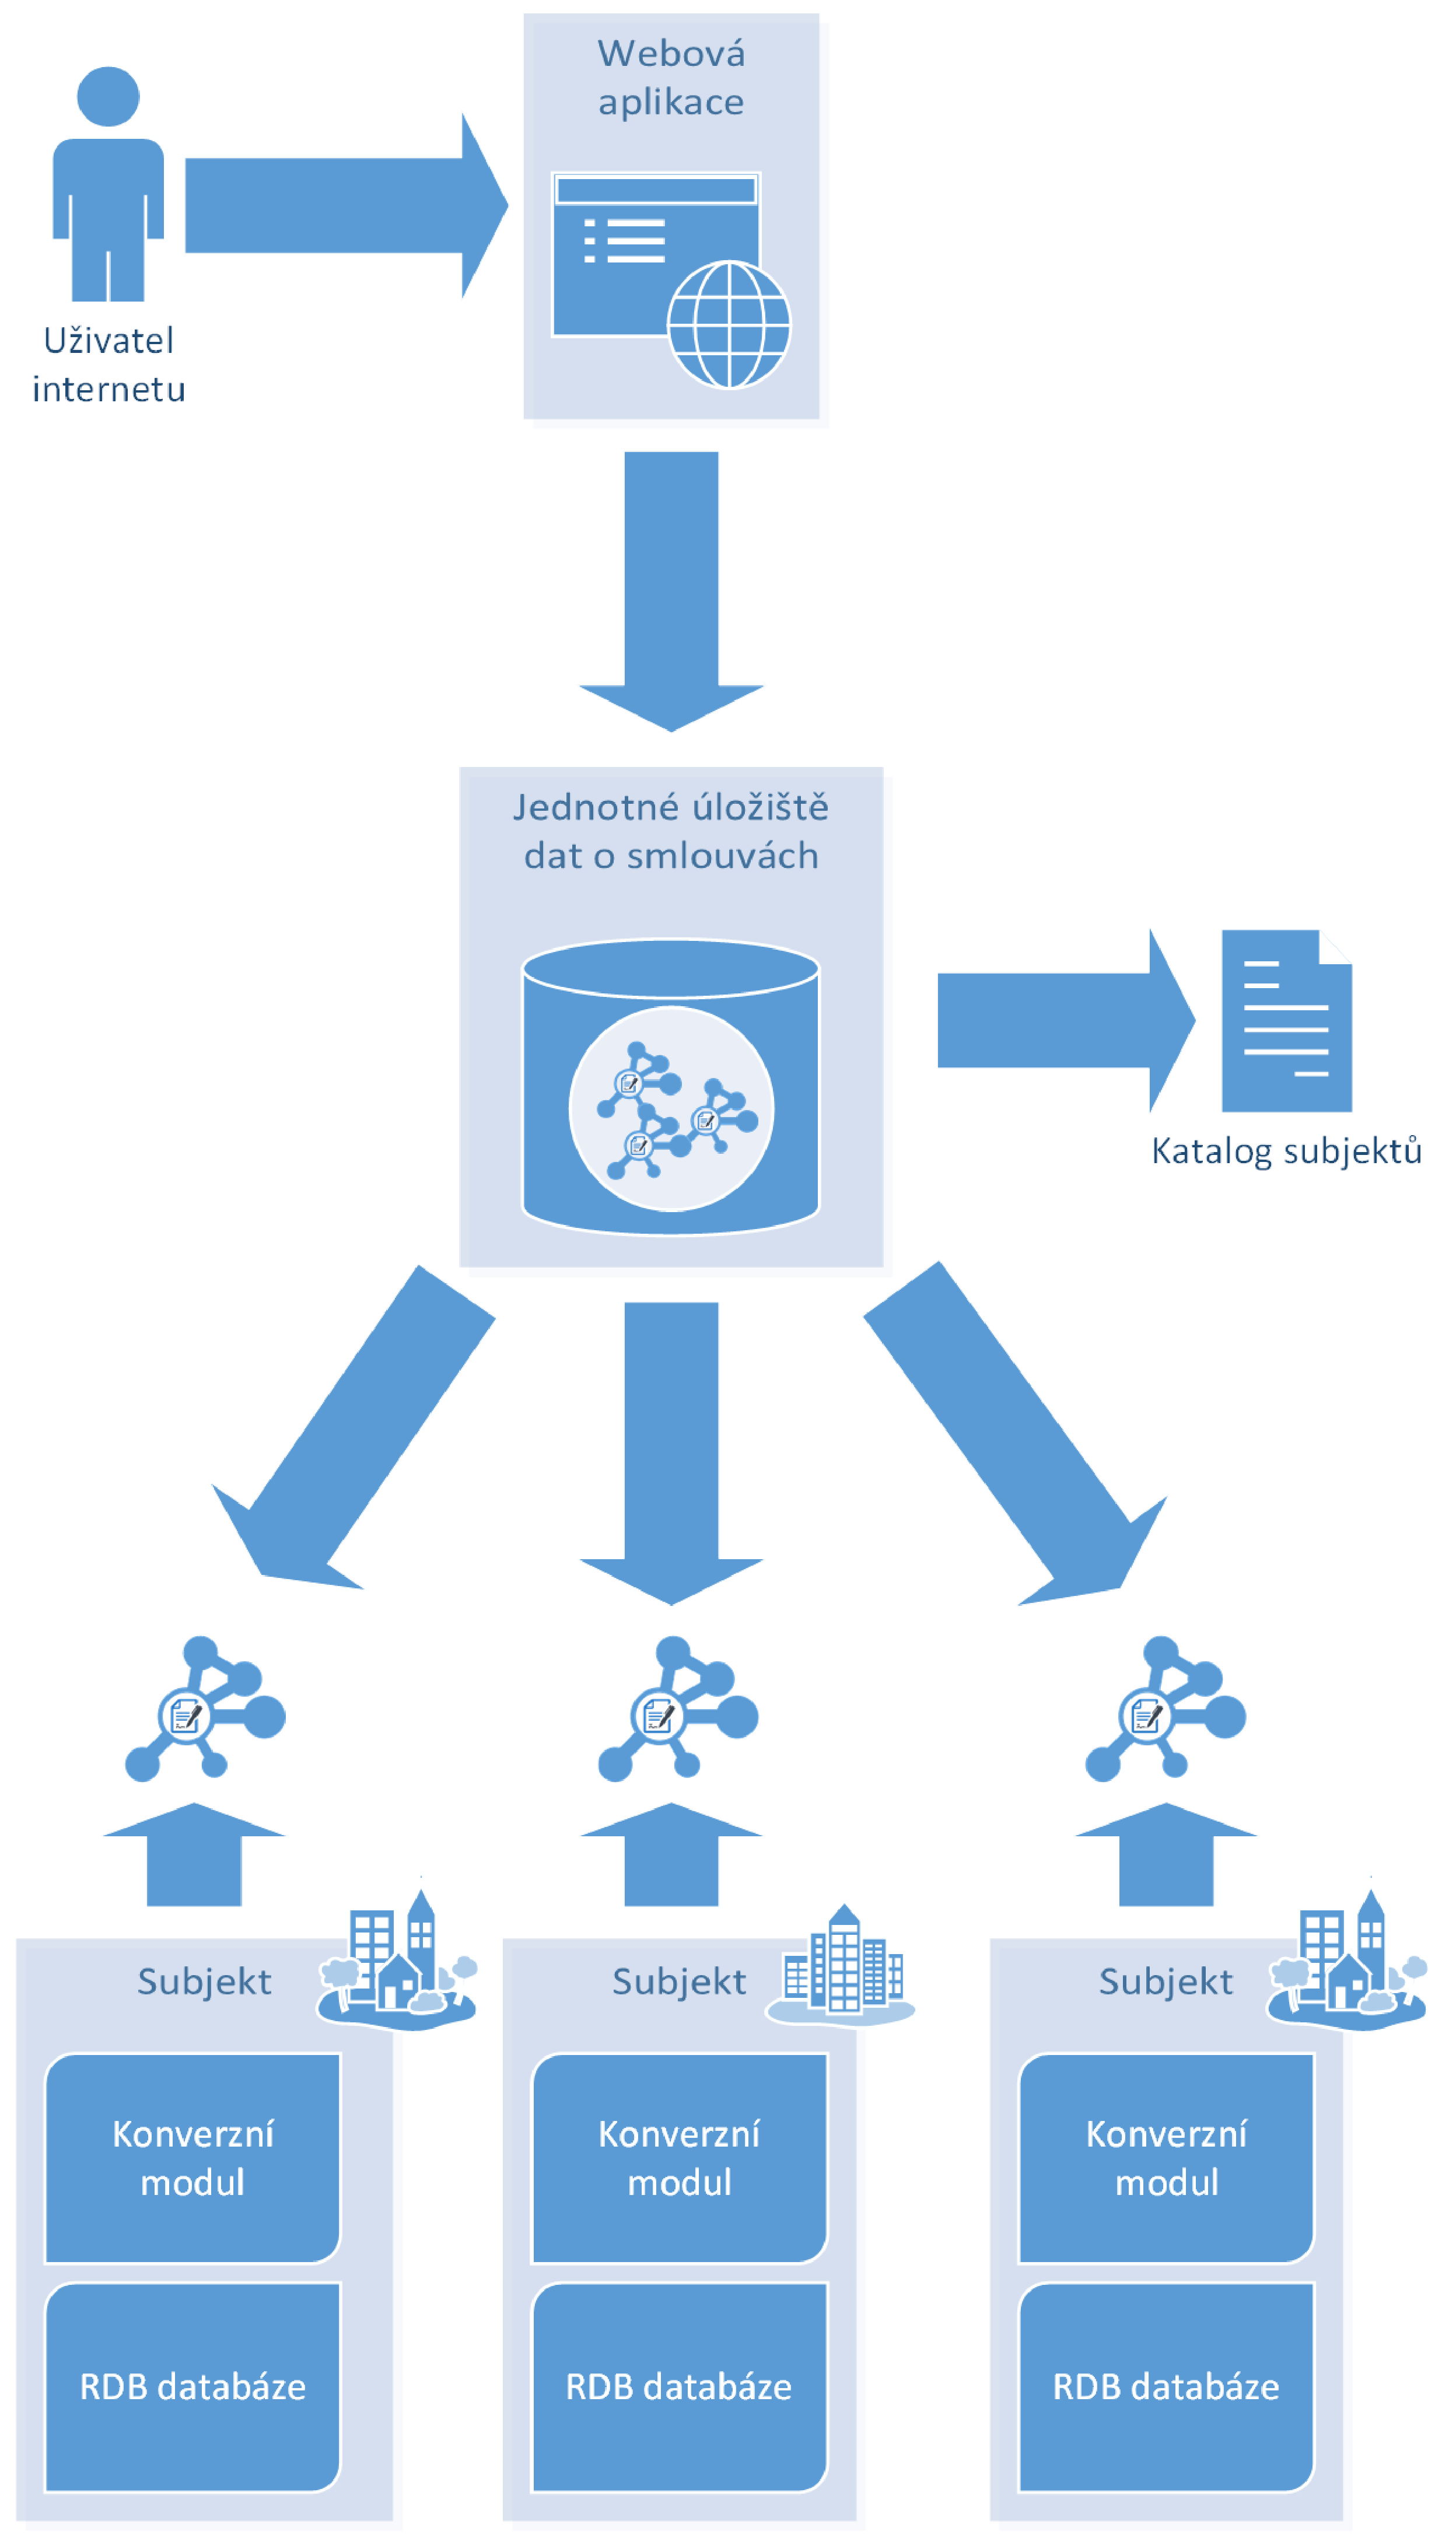
\includegraphics[width=135mm]{img/logicalView.eps}}
\caption{Základní pohled na platformu otevřených smluv (Logical view)}
\label{obr:logicalView}
\end{figure}

\begin{figure}[H]
\centerline{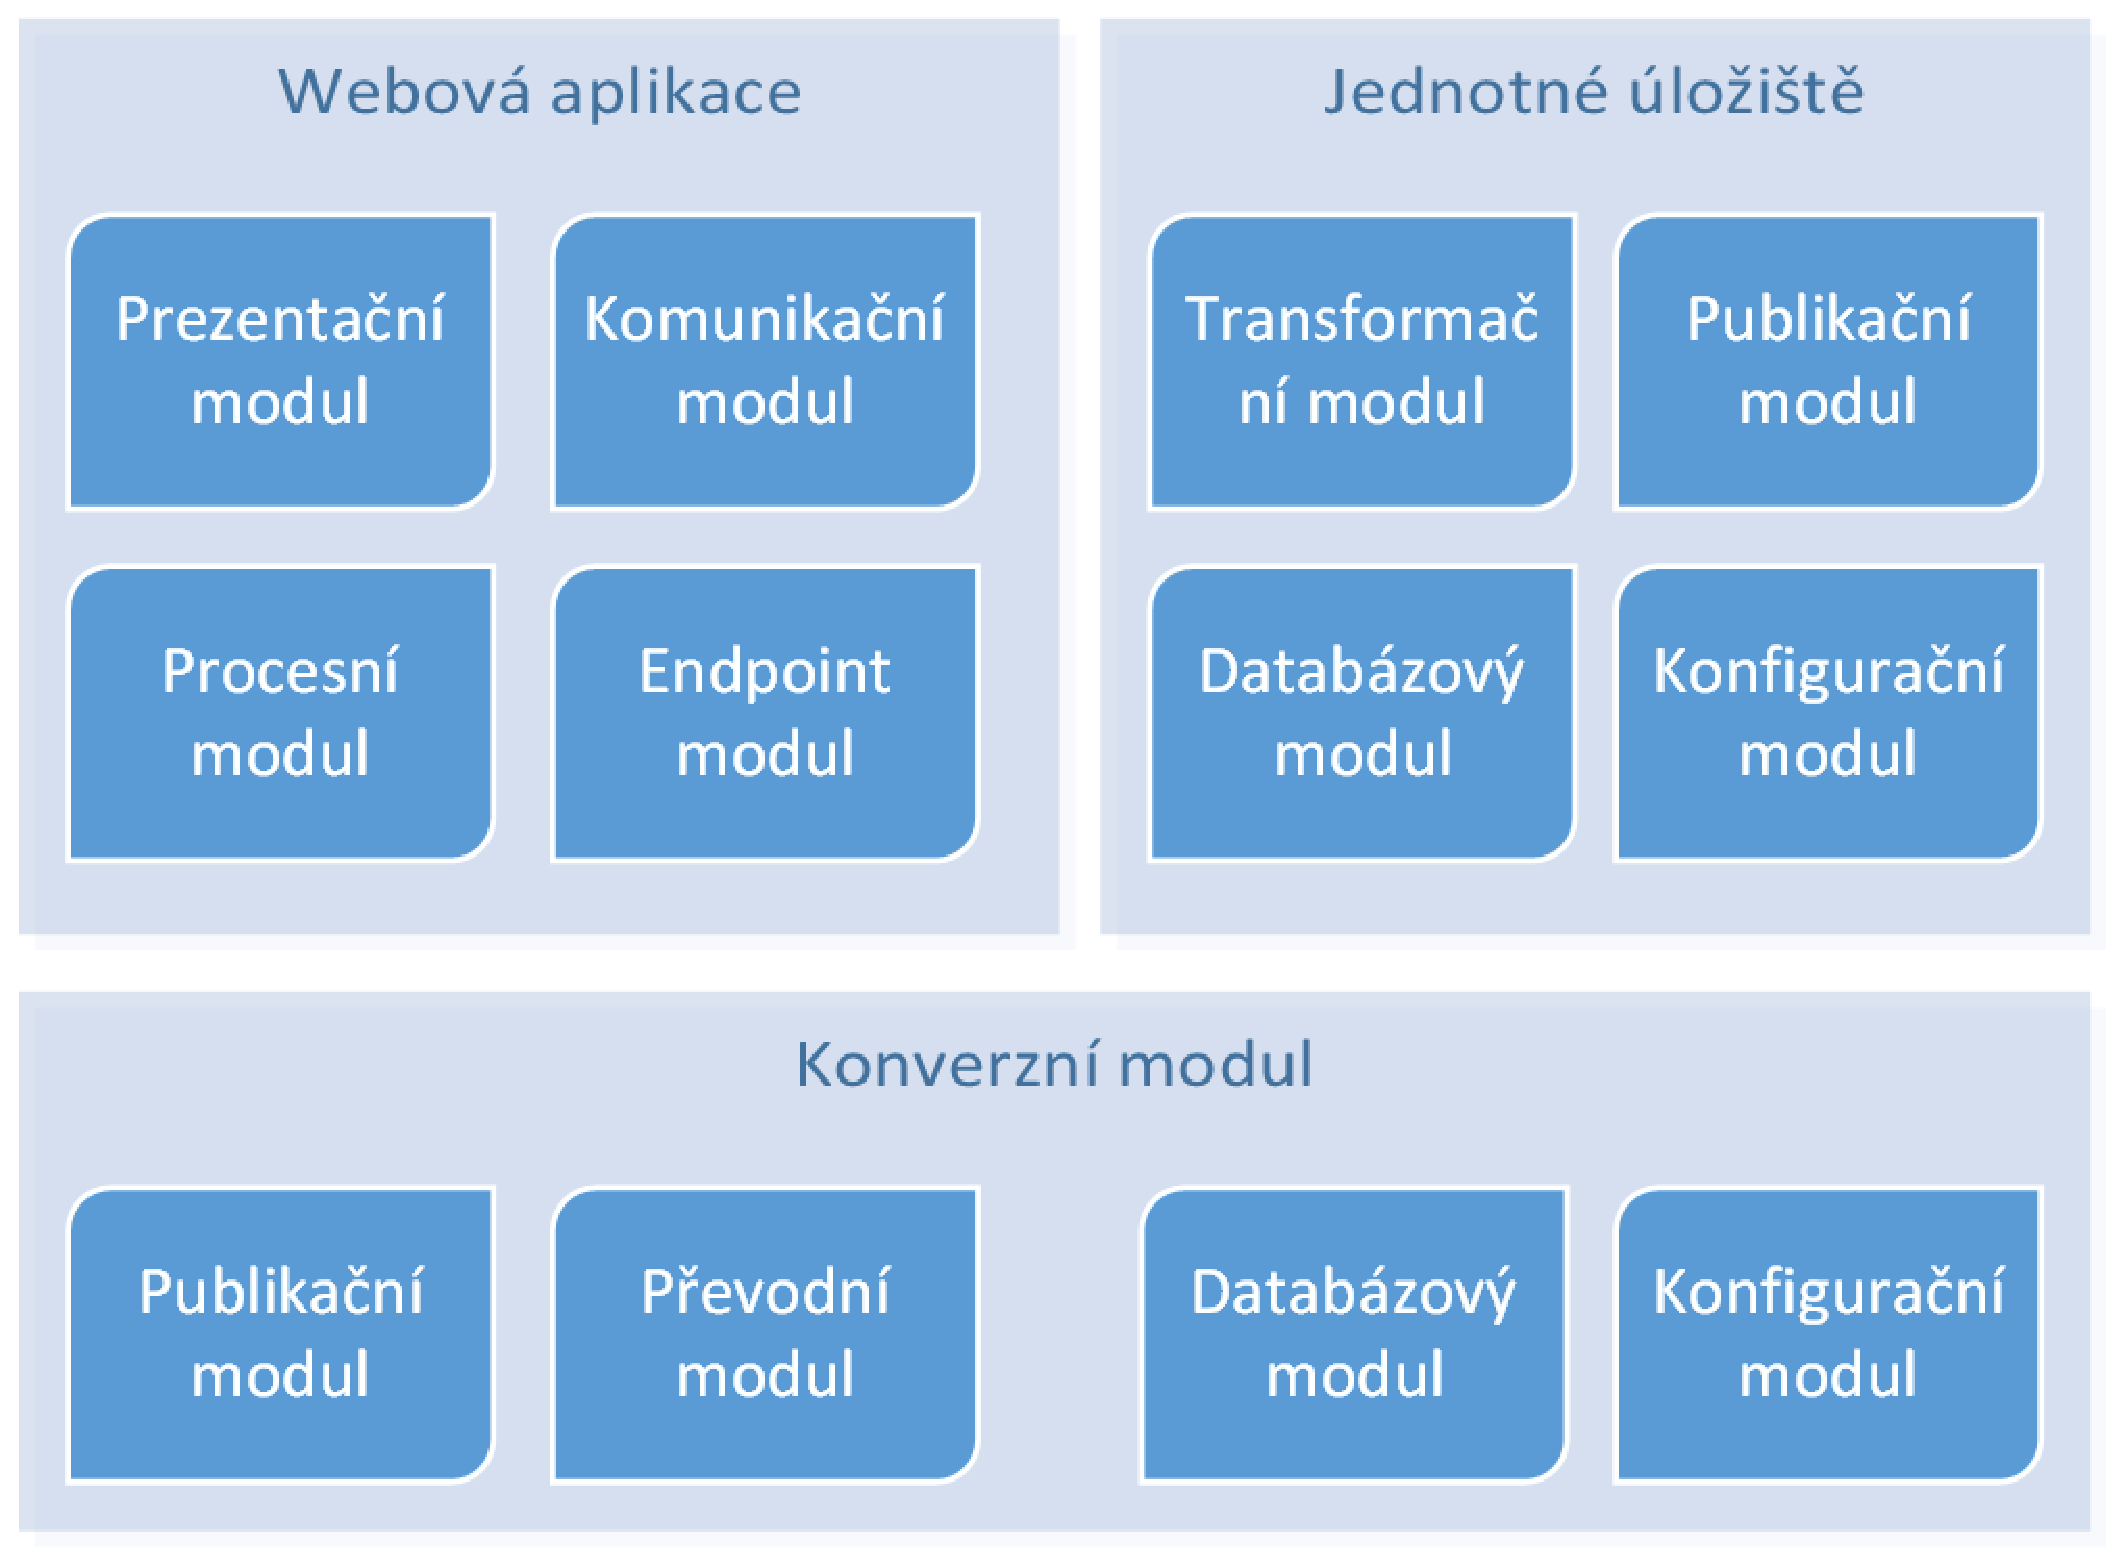
\includegraphics[width=\textwidth]{img/decompositionView.eps}}
\caption{Rozdělení platformy do modulů (Decomposition view)}
\label{obr:decompositionView}
\end{figure}

\subsection{Konverzní mechanismus}

Návrh konverzního mechanismu rozdělíme do čtyř modulů (viz Obr. \ref{obr:decompositionView}). V rámci databázového modulu bude docházet ke komunikaci mezi připojenou databází a zbytkem konverzního mechanismu. V konfiguračním modulu se očekává definování základních vlastností konverzního mechanismu, převážně potřebné vstupní údaje pro převodní modul.

\subsubsection*{Převodní modul}

Účelem tohoto modulu je převod relačních dat do RDF podoby. Nejjednodušším přístupem je manuální konverze, resp. ruční tvorba RDF výstupů. Tento přístup může být vhodný pro úzce specifické situace, avšak pro obecný přístup a možnost znovupoužití konverzního modulu vhodný není. Další možností je tvorba paralelní triplestore databáze. Relační data bychom v určitých intervalech převáděli z jedné do druhé. Tento přístup je výhodný, pokud chceme dosáhnout robustního řešení, budovat vlastní RDF úložiště, obohacovat data, přidávat další datasety apod. Klade však velké softwarové i hardwarové nároky na subjekt, vyžaduje netriviální údržbu a jedná se v podstatě o duplikovaná data z relační databáze. Poslední možností, kterou uvedeme, je tvorba wrapperu nad relační databází. Máme-li požadavek na RDF data, wrapper ho převede na ekvivalentní SQL dotaz do databáze a vrácená data převede zpět do odpovídající RDF podoby. Hlavní výhodou je, že takto uložená data jsou pouze v relační databázi a RDF data jsou tak vždy aktuální. Cílem je řešení s co nejmenší zátěží pro subjekt a s co nejlepším usnadněním znovupoužitelnosti. Ideálním řešením se tedy jeví tvorba wrapperu.

Požadovanou funkcionalitou wrapperu je namapování datového modelu relační databáze na datový standard pro otevřené smlouvy. Mezi jazyky sloužící k popsání konkrétního mapování patří např. jazyk R2RML, nebo D2RQ. Doporučeným standardem konsorcia W3C je R2RML, zvolíme tedy jazyk R2RML.

\subsubsection*{Publikační modul}

Převedená data můžeme publikovat třemi základními způsoby:

\begin{itemize}
\item Dump - veškerá data jsou zpřístupněna formou stažitelného souboru serializovaného v nějakém z RDF formátů
\item Dereferencovaná URI jednotlivých entit - každá entita je dostupná pod svým URI, typicky ve formě HTML stránky
\item API - v kontextu RDF se typicky jedná o webovou službu ve formě SPARQL endpointu umožňující libovolné dotazování nad daty.
\end{itemize}

Naší snahou je, aby vypublikovaná data mohly využívat i jiné aplikace, než pouze jednotné úložiště v rámci platformy. K tomu je ideální API. Zvolíme proto SPARQL endpoint.

Pro naplnění principů Linked Data ale potřebujeme vyřešit dereferencování URI entit. Nad SPARQL endpointem se dereference provede jednoduše tak, že každé HTTP URI odkazující na konkrétní entitu se převede na vhodný SPARQL dotaz vracející požadovaná data. 

Data budou publikována jak ve formě HTML stránky, tak v RDF formátech. Nutným základem bývá formát N-Triples a Turtle. Určíme podmínku, že pro dump je nutné umožnit i serializaci ve formátu JSON-LD z důvodu budoucí kompatibility s datovým standardem.

\subsubsection*{Anonymizace} 

Typickým problémem s publikací dat je, že mohou podléhat zákonu o ochraně osobních údajů\footnote{https://www.uoou.cz/anonymizace-osobnich-udaju/d-1764}. Některá data je proto před zveřejněním nutné anonymizovat. Proces a řešení anonymizace není předmětem této práce. Řekněme, že platforma počítá s tím, že subjekt si anonymizaci údajů vyřeší na své straně.

\subsection{Jednotné úložiště}

Agendou jednotného úložiště bude sbírat data vypublikovaná jednotlivými subjekty. Zapojené subjekty budeme řešit formou datového katalogu, kde budou odkazy na umístění požadovaných datasetů. Úložiště pak v definovaném intervalu stáhne datasety podle datového katalogu a uloží je do triplestore databáze.

Dekompozici do modulů je možné vidět na Obr. \ref{obr:decompositionView}. Konfigurační a databázový modul má podobný význam jako v konverzním mechanismu.

\subsubsection*{Transformační modul}

V prvním kroku je třeba načíst jednotlivé datasety subjektů. Odkazy na konkrétní datasety budou reprezentované ve formě datového katalogu. Samotný katalog budeme zapisovat v RDF a serializovat do formátu Turtle. Využijeme k tomu ontologii Data Catalog Vocabulary. Příklad datového katalogu lze vidět v kódu \ref{lst:subject_catalog}.

V dalším kroku je třeba vyřešit otázku heterogenity dat. Platforma by principiálně měla umět přijímat RDF data nejen od subjektů zpracovaná konverzním modulem, ale i jakákoli jiná RDF data splňující datový standard a reflektující definovanou RDF ontologii. Jednotlivé entity by ale měly být identifikované podle vzoru z kapitoly~\nameref{sec:kap4}. To nám zaručí, že žádné dvě entity různých subjektů nebudou mít díky rozdílným doménám stejné URI. 

Díky tomu tak můžeme v rámci závěrečného kroku data slít dohromady a uložit do triplestore databáze.

\lstinputlisting[label=lst:subject_catalog, caption=Datový katalog pro jednotné úložiště, language=XML]{code/subject_catalog.ttl}

\subsubsection*{Publikační modul}

Úložiště by mělo data poskytovat jak k webovému prohlížení, tak skrze API k využití v aplikacích. Tento požadavek vyřešíme vystavením SPARQL endpointu.

\subsection{Propojená datová síť}

Nad jednotným úložištěm může vznikat celá řada aplikací využívajících data o smlouvách. Díky propojení smluv se souvisejícími daty, tak můžeme kontext smluv rozšířit o další informace, resp. demonstrovat výhody principů Linked Data jako propojené datové sítě.  

V rámci kapitoly 4 jsme definovali odkaz na veřejnou zakázku (pco:Contract) v rámci smlouvy, resp. predikát pco:publicContract ze smlouvy (třída cn:Contract) a odkaz na ekonomický subjekt (gr:BusinessEntity) pomocí predikátů owl:sameAs ze Smluvní strany a Vydavatele (třídy foaf:Organization a gr:BusinessEntity). Nyní si položme otázku, s jakými dalšími relevantními zdroji můžeme data na základě definovaných odkazů dále propojit.

Navrženou datovou síť propojených objektů můžeme vidět na Obr. 6.3. Z každého datasetu (v oválných blocích) vede hrana k vlastnímu objektu. Z nich pak vychází vybrané predikáty odkazující na entitu dalšího datasetu. 

Výchozím bodem je entita ekonomického subjektu (gr:BusinessEntity) uprostřed. Konkrétně se jedná o registrované organizace, jejichž data vychází z údajů na Profilu zadavatele, z ARESu a dalších zdrojů. Z této entity využijeme predikáty (s:address) k propojení s adresou (s:PostalAddress) z ARESu. Z adresy, pak získáme informaci o adresním místu (s:Place) z RUIANu pomocí predikátu ruianlink:adresni-misto.

Z entity ekonomického subjektu můžeme získat informaci o odpovídajícím objektu reprezentovaném v rámci orgánů veřejné moci díky zpětnému odkazu reprezentovanému predikátem ovm:business-entity. 

Propojení dosáhneme také mezi ekonomickým subjektem a veřejnou zakázkou (pco:Contract). Z veřejné zakázky využijeme odkazu na zadavatele, resp. predikátu (pco:contractAuthority). Díky tomu můžeme zjistit údaje o veřejných zakázkách jednotlivých ekonomických subjektů, kde vystupují v roli zadavatele.

Vydavatel smluv (foaf:Organization) je často veřejná instituce mající svoji stránku na DBpedii. Nedisponujeme však přímým odkazem na konkrétní reprezentaci vydavatele v DBpedii. Můžeme ale položit SPARQL dotaz, zdali v DBpedii existuje instituce s daným konkrétním jménem (porovnáním predikátů gr:legalName vydavatele a rdfs:label z DBpedie). Nejedná se tedy o přímé propojení, ale o další možnost, jak kontext smluv obohatit o další informace.

\begin{figure}[H]
\centerline{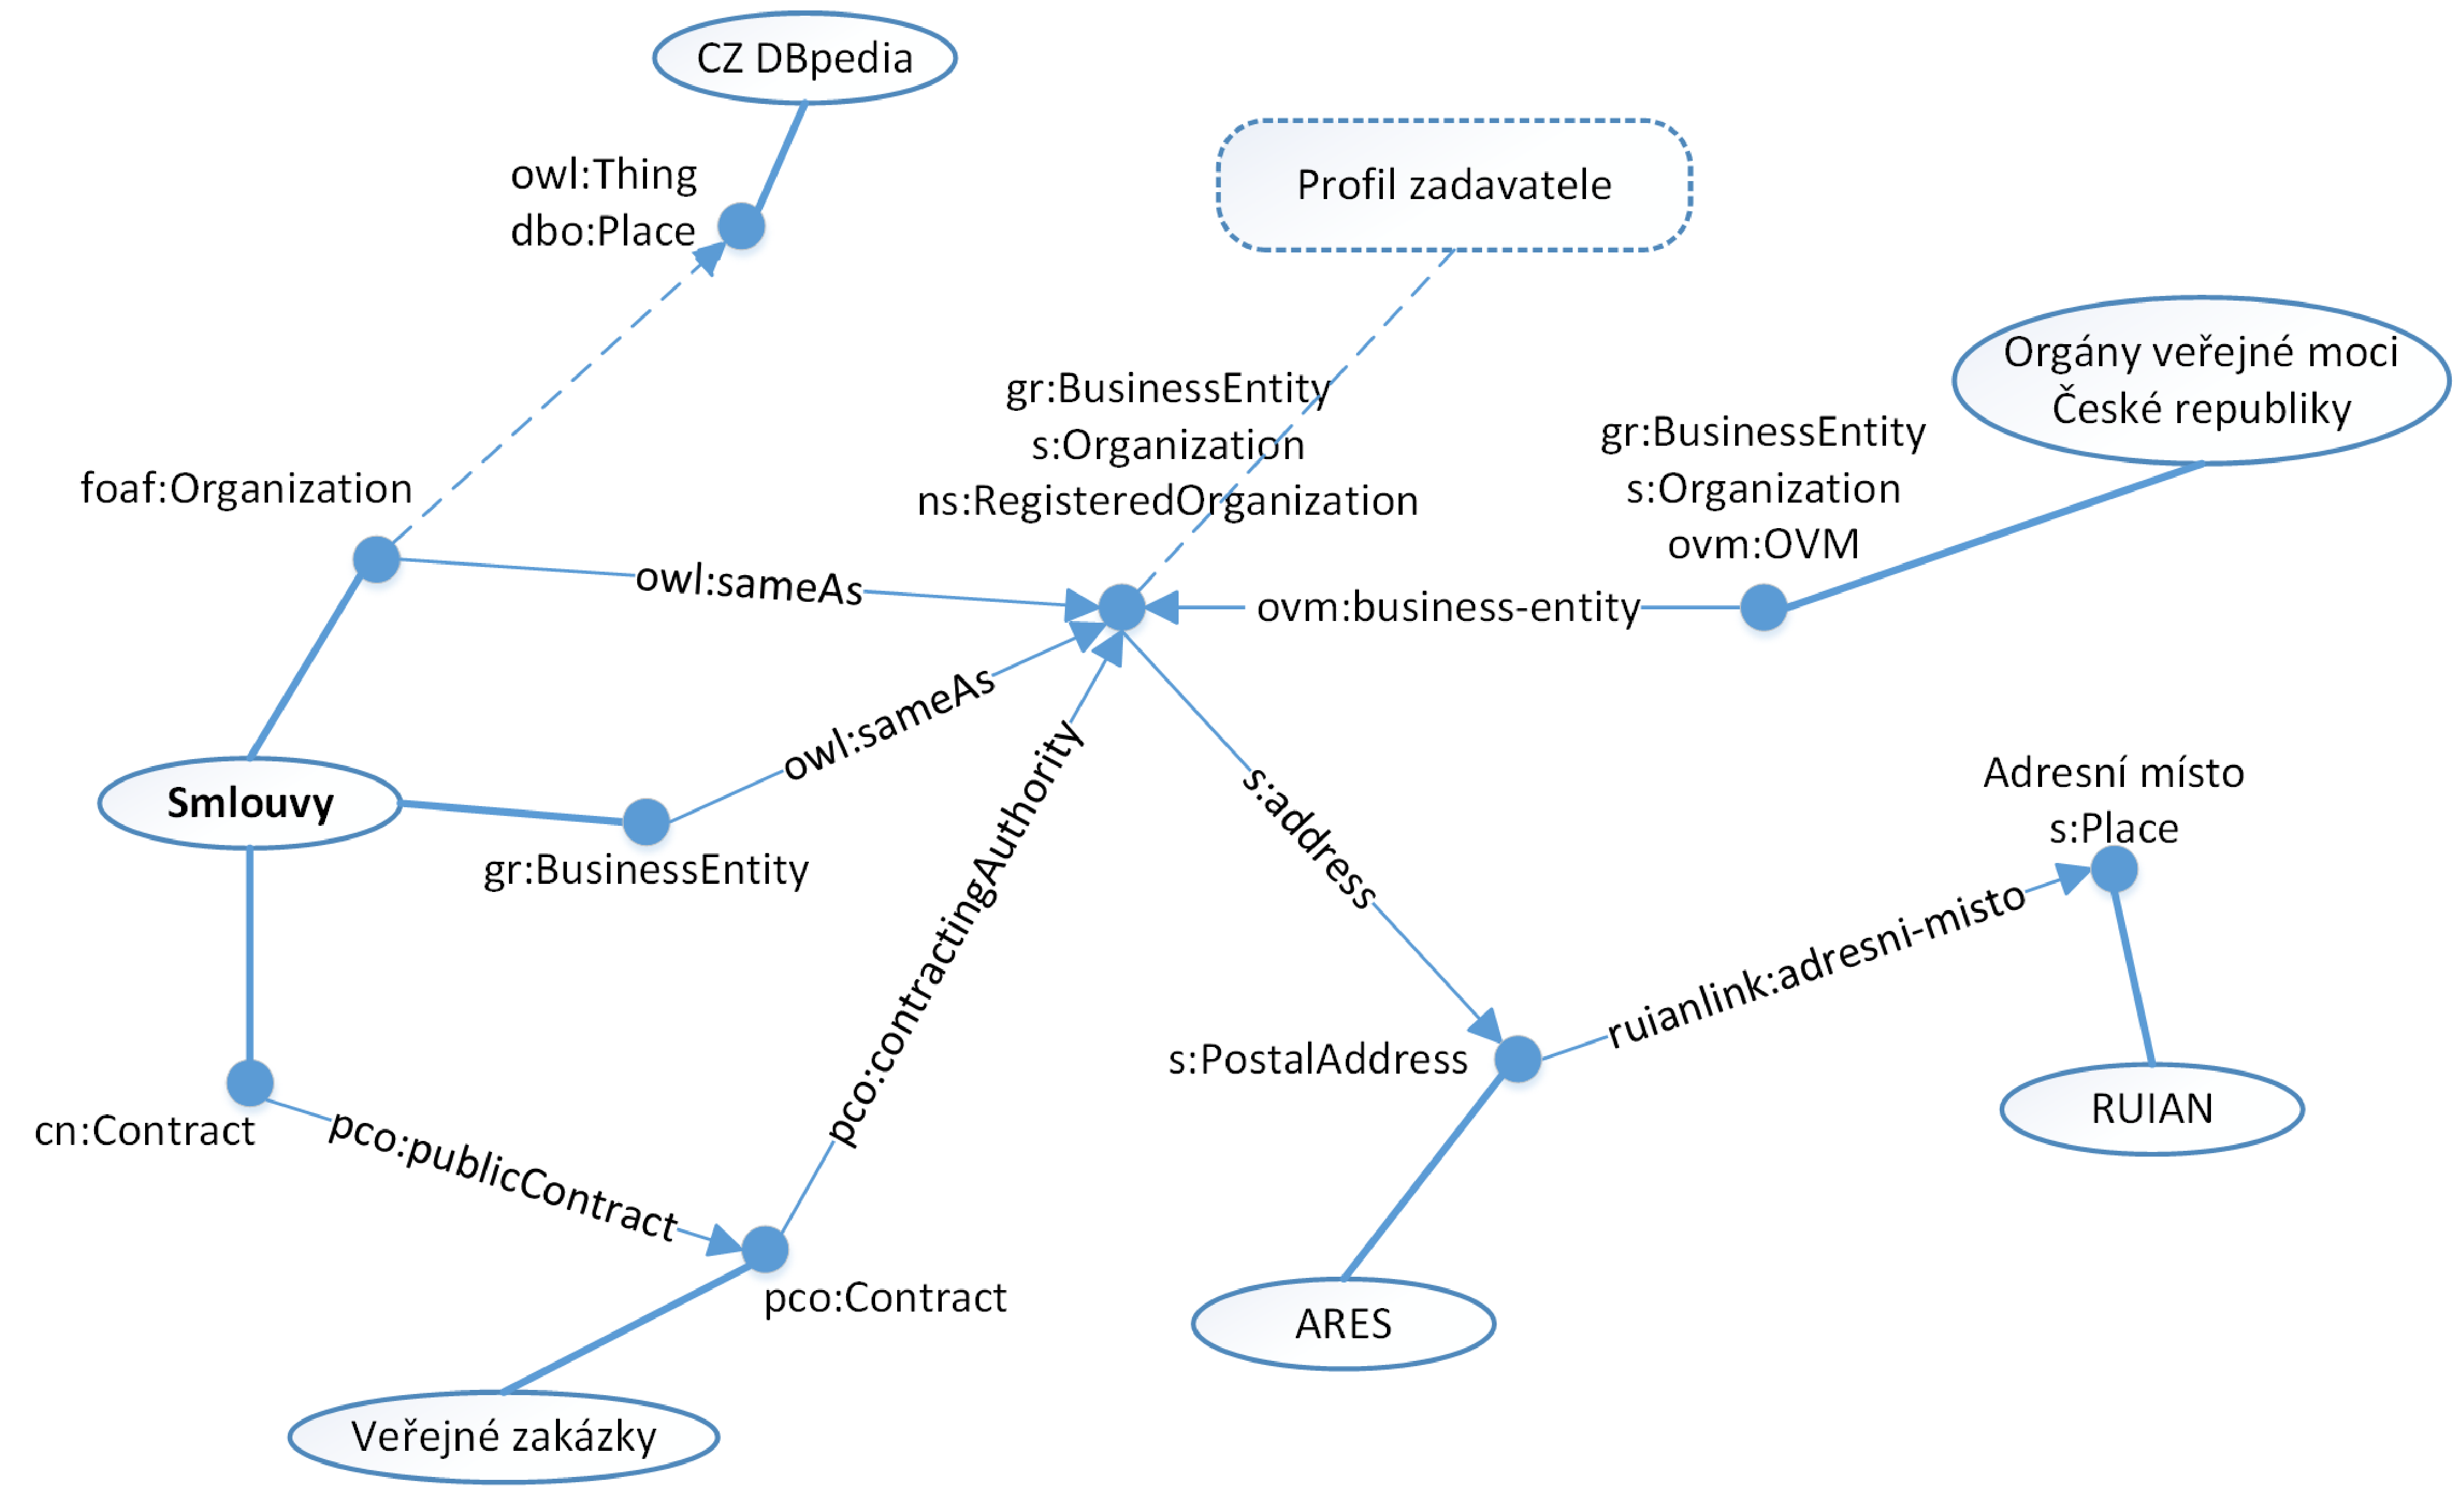
\includegraphics[width=\textwidth]{img/architectureLinks.eps}}
\caption{Propojená datová síť}
\label{obr:architectureLinks}
\end{figure}

\subsection{Webová aplikace}

Úkolem webové aplikace je nad jednotným úložištěm zpřístupnit údaje o smlouvách k prohlížení koncovým uživatelům. Řešení rozdělíme do čtyř modulů (viz Obr. \ref{obr:decompositionView}).

\subsubsection*{Endpoint modul}

V rámci tohoto modulu definujeme napojení na požadované zdroje dat v podobě SPARQL endpointů.

\subsubsection*{Procesní modul}

Úkolem tohoto modulu je načíst požadované údaje o smlouvách a přiřadit k nim údaje z rozšířeného kontextu navrženého v minulé kapitole. Cílem je tedy získat a sjednotit informace z několika zdrojů dat. Existuje několik přístupů, jak se nad požadovanými daty dotazovat\footnote{Předpokládejme, že aplikace bude obsahovat serverovou část.} - z klientské části aplikace, nebo ze serverové. Z důvodu dalšího zpracování dat se jeví vhodnější serverové dotazování. Samotné dotazy můžeme pokládat také různými způsoby. Jednou z možností je distribuované dotazování, kdy se v rámci jednoho dotazu můžeme odkazovat na více zdrojů. Další možností je se nad každým zdrojem dotazovat zvlášť, resp. sadou dotazů. V souladu s principy Linked Data zvolíme sadu dotazů nad jednotlivými SPARQL endpointy. Výhodou je, že problém jednoho zdroje by neměl ovlivnit výsledky z ostatních zdrojů. 

Nad SPARQL endpointy můžeme získávat data buď ve formě RDF (příkaz Construct), nebo v tabulkové formě (příkaz Select). Účelem je zobrazení dat uživateli často právě ve formě tabulek. Volba příkazu Select je tedy lepší volbou.

\subsubsection*{Komunikační modul}

Agendou komunikačního modulu je výměna dat mezi procesním a prezentačním modulem. Modul zpracuje požadavky z prezentačního modulu a volá konkrétní funkce procesního modulu. Výsledná data pak pošle prezentačnímu modulu k zobrazení. Rozhraní pro přenos by mělo být ve standardizovaném datovém formátu\footnote{Typicky v XML, nebo JSON}.

\subsubsection*{Prezentační modul}

Účelem tohoto modulu je zobrazování dat uživateli. Výchozím bodem je nabídnout seznam smluv. Úvodní obrazovkou bude tedy pohled s úvodními informacemi a souhrnným seznamem smluv. Z každé položky půjde přejít jak do detailu konkrétní smlouvy, tak do detailu jejího vydavatele. Detail smlouvy zobrazí podrobné informace o zvolené smlouvě, včetně jejích verzí, smluvních stran, příloh, dodatků a milníků. Ze subjektů a smluvních stran majících vyplněný IČ půjde přejít na seznam veřejných zakázek, ve kterých subjekt vystupuje. Detail vydavatele nabídne podrobnější informace o zvoleném publikujícím subjektu. Součástí detailu vydavatele bude také seznam jeho smluv. Z tohoto seznamu půjde také přejít na detaily jednotlivých smluv.

\begin{figure}[H]
\centerline{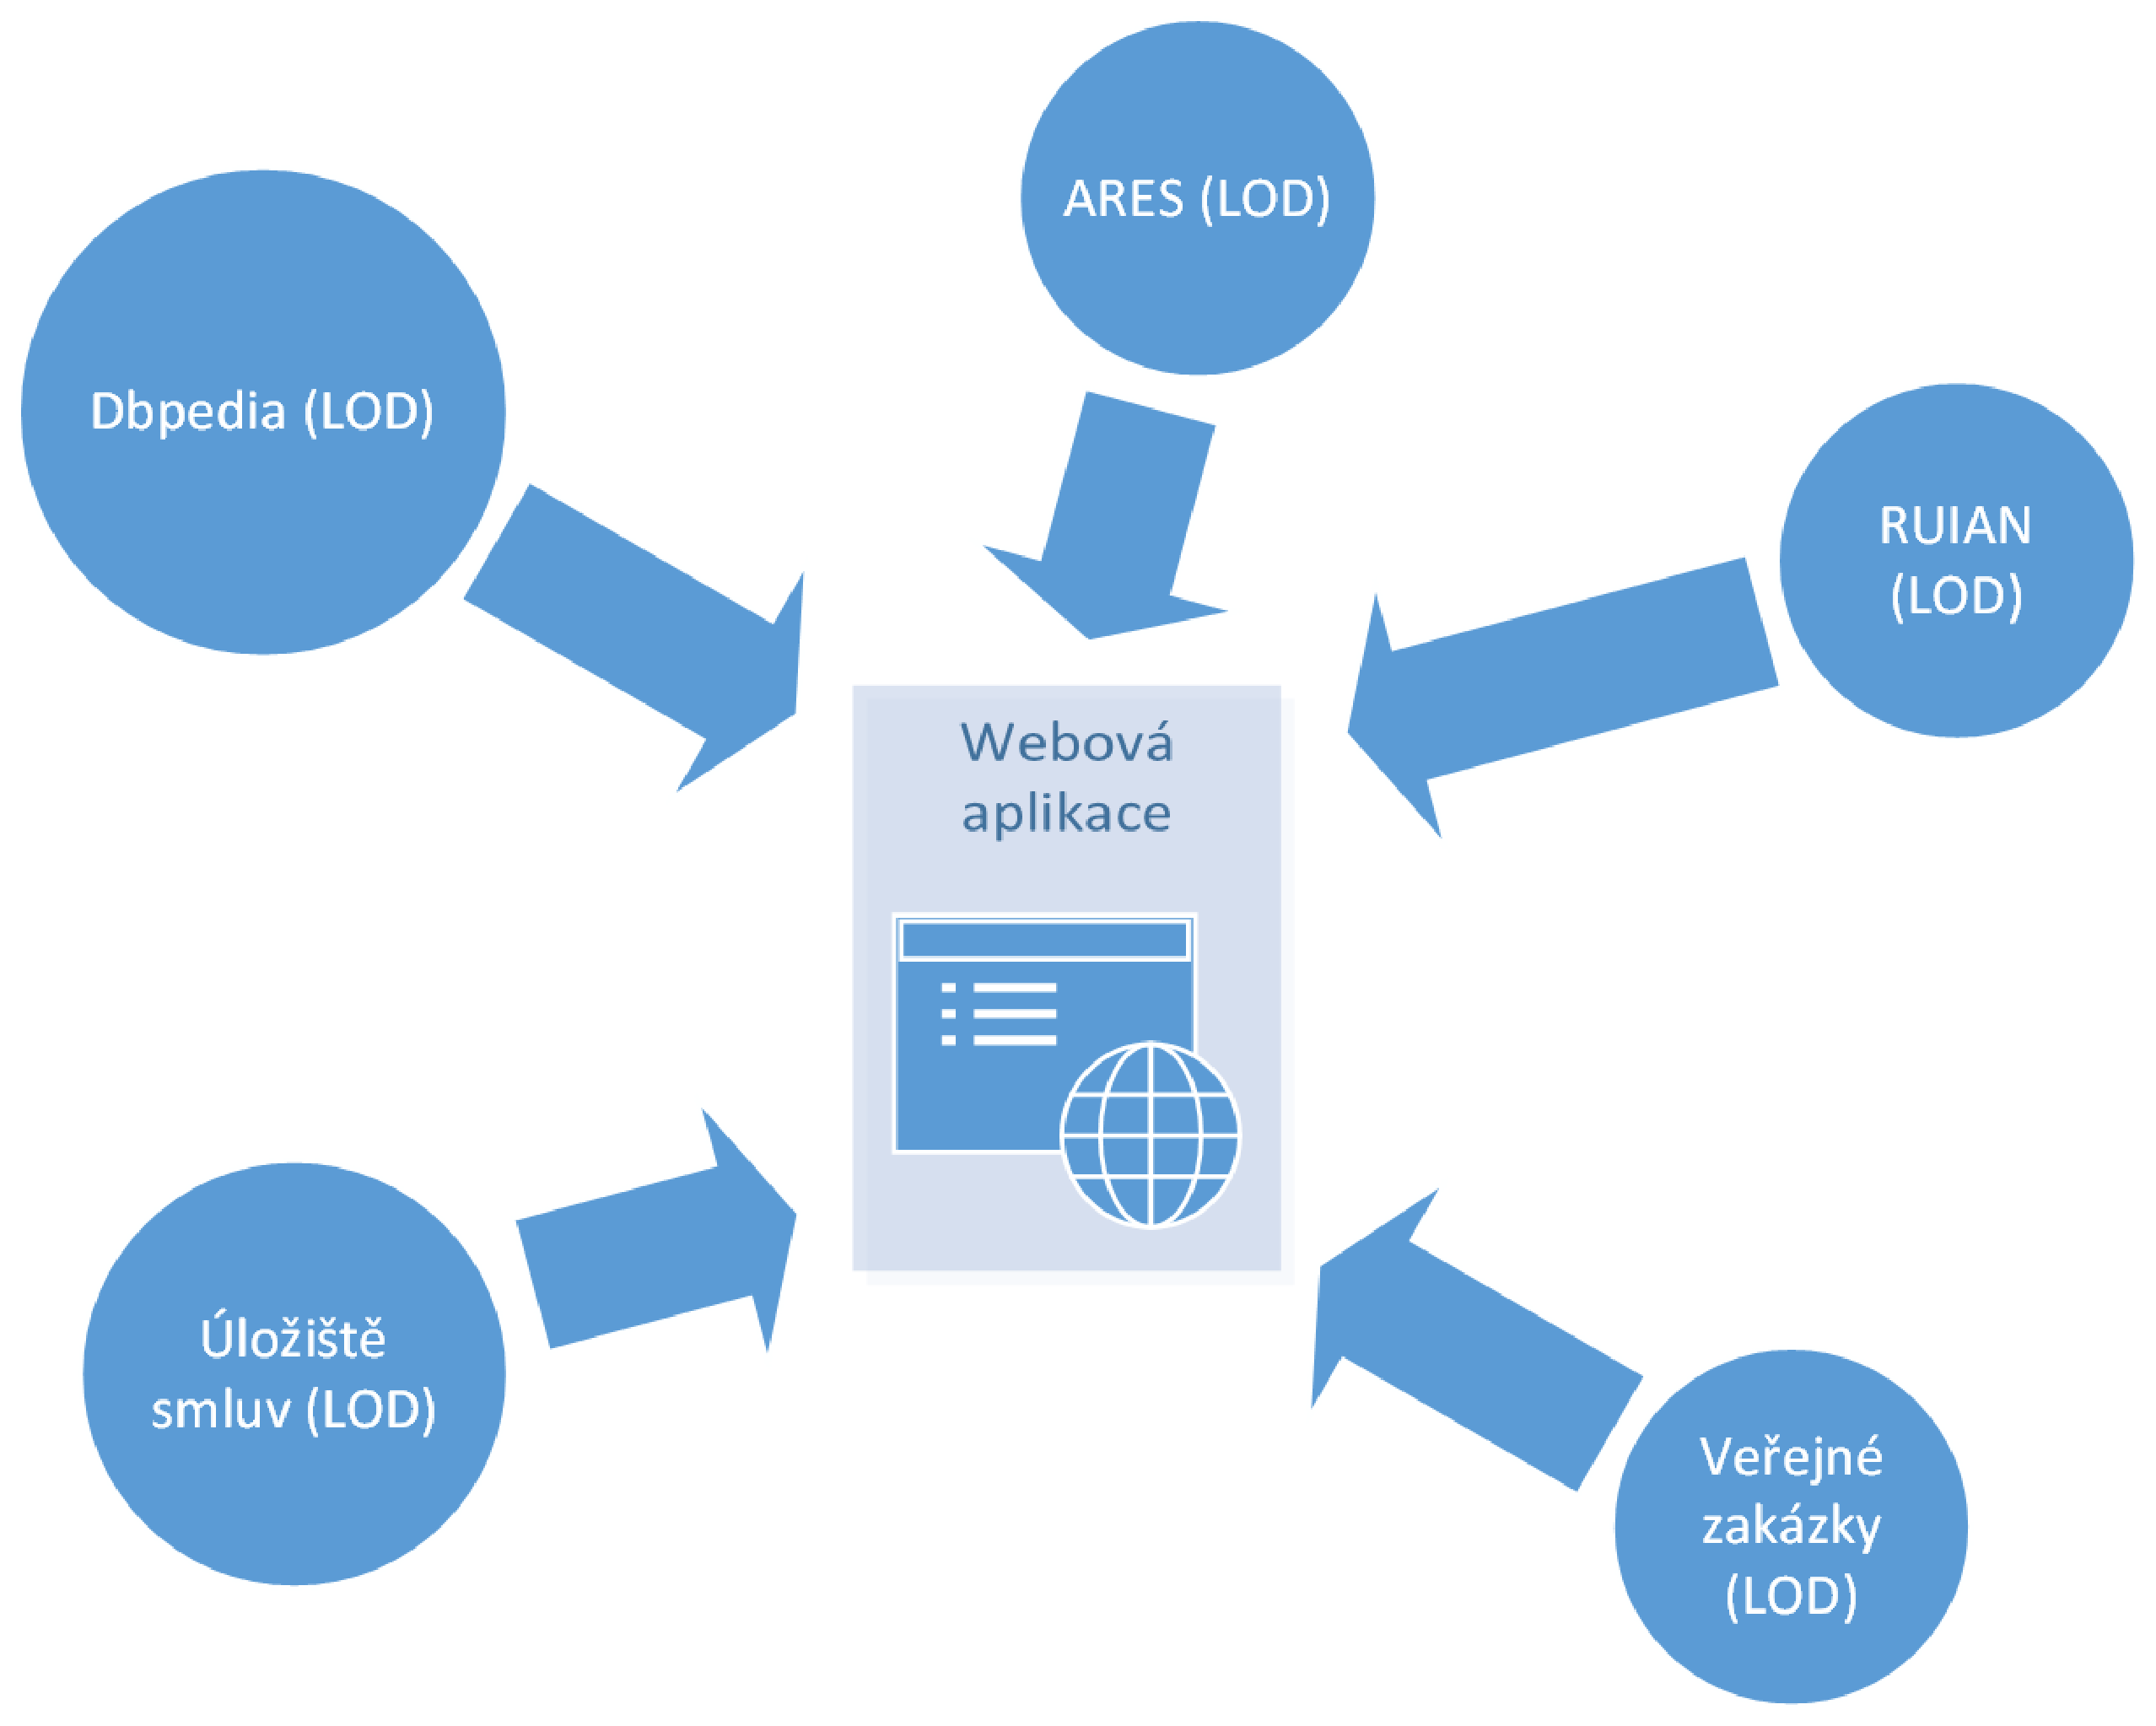
\includegraphics[width=120mm]{img/linkedDataAdv.eps}}
\caption{Obohacený kontext smluv díky propojeným datům}
\label{obr:linkedDataAdv}
\end{figure}
\chapter{Implementace platformy}

\section{Konverzní mechanismus}

Prvním krokem ve vývoji konverzního modulu je volba a analýza zdrojové platformy. Je třeba zpracovat danou doménu a především se seznámit se strukturou datového modelu. Druhým krokem je tvorba R2RML mapovacího skriptu. Závěrečným krokem je samotná implementace konverzního mechanismu. Tento postup uvádíme proto, že jednotlivé kroky lze řešit nezávisle. Např. definované R2RML mapování nad konkrétní doménou může posloužit jako podklad k různým aplikacím pracujícím s R2RML. 

\subsection{Munis ESML}

Jako zdroj pro implementaci konverzního mechanismu byl zvolen modul Munis ESML. Jedná se o část informačního systému pro města a obce společnosti Triada. spol. s.r.o.

Účelem modulu Munis ESML je evidování odběratelských i dodavatelských smluv. Nabízí přehledné vyhledávání, statistiky, hlídání termínů, nebo možnost přiřadit smlouvy jednotlivým grantům, projektům či veřejným zakázkám (viz. Obr \ref{obr:munisEsml}).

\begin{figure}[H]
\centerline{\includegraphics[width=\textwidth]{img/munisEsml.eps}}
\caption{Modul ESML}
\label{obr:munisEsml}
\end{figure}

\newpage

\subsubsection{Struktura datového modelu}

Základem datového modelu jsou entity \textit{Smlouva} a \textit{Verze smlouvy}. Smlouva je základním stavovým objektem s hierarchickou strukturou. Vycházíme z předpokladu, že dodatek ke smlouvě je také smlouva, proto definujeme:

\begin{itemize}
\item Entita \textit{Smlouva} na kořenové úrovni popisuje smlouvu
\item Každý syn entity \textit{Smlouva} je jejím dodatkem
\end{itemize}

Každá smlouva je verzovaná, resp. entita Smlouva může mít několik \textit{Verzí smlouvy}. Entita \textit{Verze smlouvy} reprezentuje popisné údaje \textit{smlouvy}. Dále obsahuje vazby na \textit{rozdělovník, smluvní strany, milníky, transakce, externí kontakty a číselníky}, viz Obr. \ref{obr:munisDatamodel}.

Každá \textit{Verze smlouvy} může obsahovat hierarchickou strukturu příloh. Každá entita \textit{Příloha smlouvy} reprezentuje fyzický soubor. Přílohy definujeme takto:

\begin{itemize}
\item Každá \textit{Verze smlouvy} může mít pouze jednu kořenovou přílohu
\item Kořenová příloha je hlavním dokumentem obsahujícím text smlouvy
\item Ostatní jsou dílčími přílohami
\end{itemize}

Entity \textit{Změna stavu smlouvy, Rozdělovník, Rozdělovník smluv přístup, Rozdělovník smluv přístup historie} nejsou pro naše účely důležité, proto je dále v textu nebudeme zmiňovat.

K popsání informací o smlouvách budeme ještě využívat tabulku TRI\_UZIVATEL reprezentující uživatele systému a TRI\_ORGADR reprezentující adresu útvaru. 

\subsubsection{Omezení vůči standardu}

V porovnání s datovým standardem pro smlouvy disponuje Munis ESML několika omezeními:

\begin{itemize}
\item Modul nepodporuje objednávky a faktury
\item Transakce nejsou implementovány - s podporou transakcí a obecně smluvního plnění se počítá do dalších verzí 
\end{itemize}

\begin{figure}[H]
\centerline{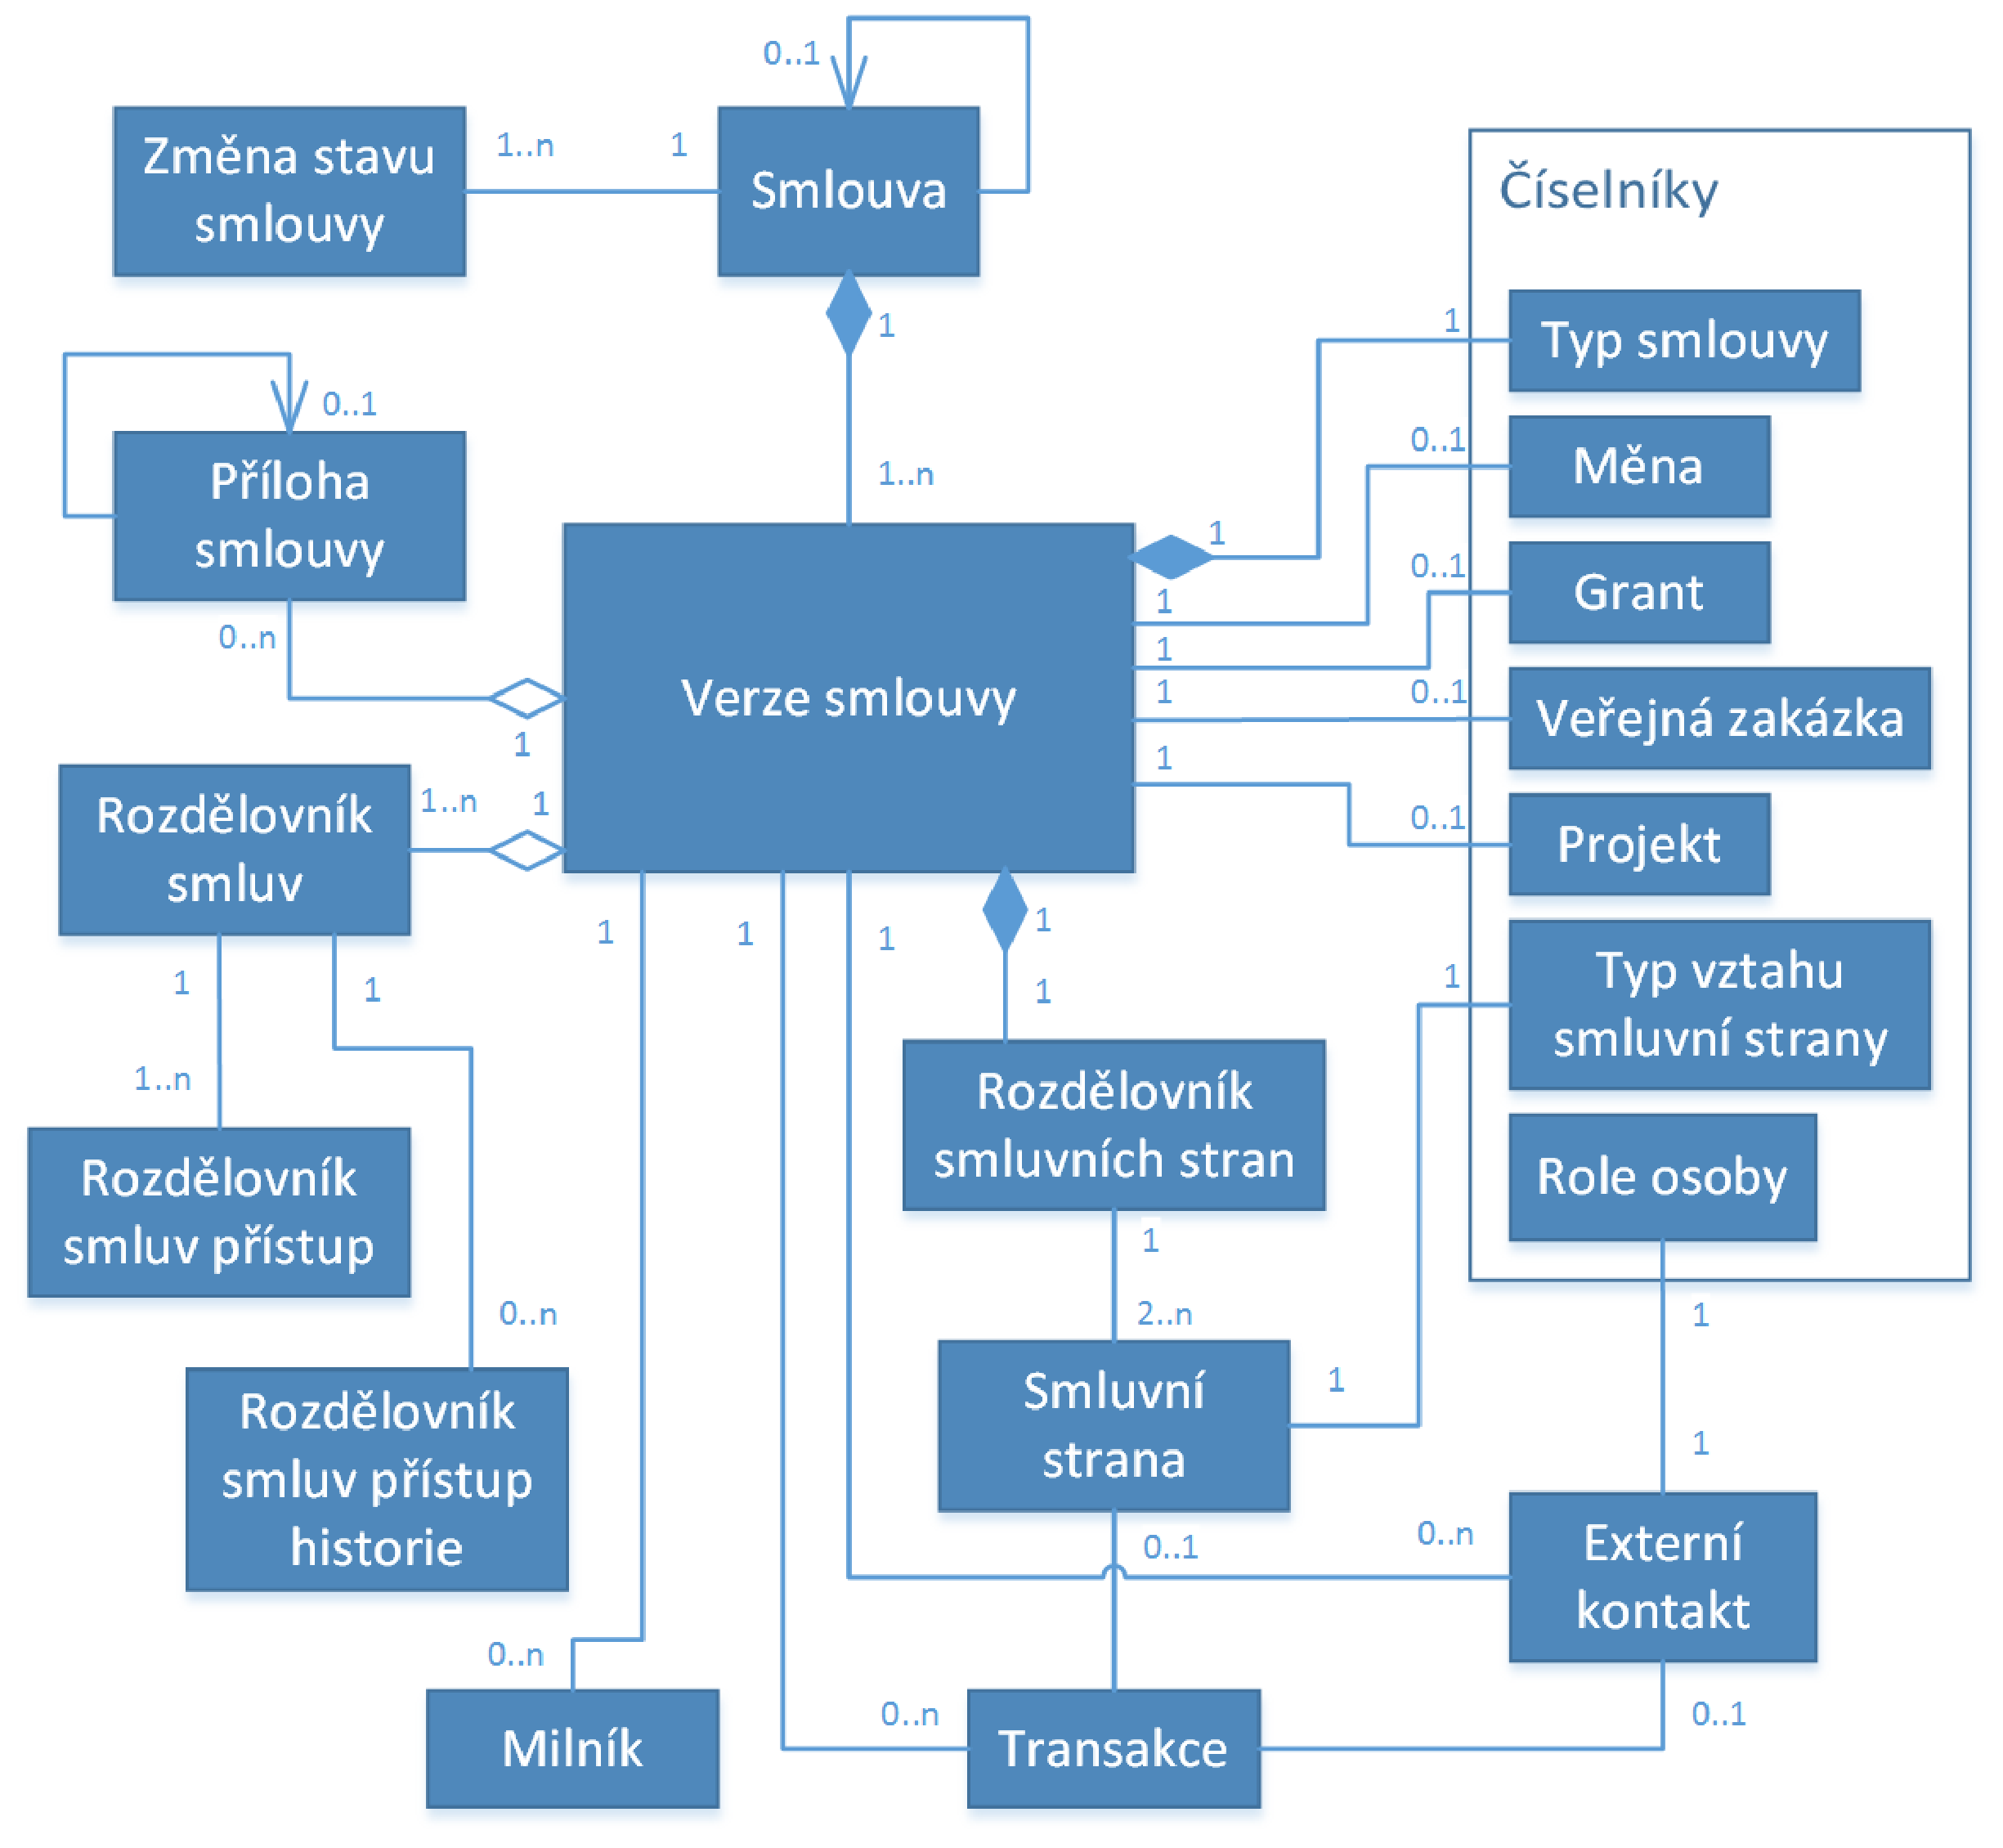
\includegraphics[width=\textwidth]{img/munisDatamodel.eps}}
\caption{ Zjednodušený datový model (bez atributů) Munis ESML}
\label{obr:munisDatamodel}
\end{figure}

\subsection{R2RML mapování}

Pomocí R2RML skriptu můžeme namapovat konkrétní sloupce z databázových tabulek na RDF predikáty. Pro složitější mapování umožňuje R2RML definovat vlastní SQL pohledy (SQL Views) nad relační databází, čehož využijeme. Pro každou entitu v rámci datového standardu proto definujeme vlastní SQL pohled. Výsledný R2RML skript lze nalézt v příloze E.

V následující části je schématicky naznačeno mapování položek. Každé entitě přiřadíme URI a typ. Následně se namapují jednotlivé položky na predikáty. Vycházíme z informací řečených v kapitole~\nameref{sec:kap4}.

\subsubsection{Smlouva}

Na obr. \ref{obr:munisSmlouva} můžeme vidět vybraný seznam tabulek a jejich atributů z datového modelu Munis ESML, které použijeme k mapování smlouvy.

\begin{figure}[H]
\centerline{\includegraphics[width=\textwidth]{img/munisSmlouva.eps}}
\caption{R2RML mapování - tabulky k mapování smlouvy}
\label{obr:munisSmlouva}
\end{figure}

Prvním krokem je přiřazení URI entitě. URI je kombinací atributu ID tabulky ESMLUV\_SMLOUVA a číslem její verze, resp. atributem PORADIVERZE tabulky (ESMLUV\_VERZESMLOUVY). Typem entity je třída cn:Contract.

\begin{itemize}
\item \textbf{URI entity} - \textit{http://[domain]/contract/\{ID\}/\{PORADIVERZE\}}
\item \textbf{Typ} - cn:Contract
\end{itemize}

\paragraph*{Konstanty}

Některé položky budou vždy obsahovat konstantní hodnotu:

\begin{itemize}
\item \textbf{dcmi:type} - s hodnotou \uv{Smlouva}
\item \textbf{cn:priceAnnual} - Nelze určit roční částku, proto vždy \uv{false}
\item \textbf{cn:funding} - Vychází zatím z nedefinovaného číselníku datového standardu, mapujeme nepovinně konstantní hodnotu \uv{vlastní}
\end{itemize}

\paragraph*{Mapované položky}

\begin{itemize}
\item \textbf{cn:anonymised} - Atribut ANONYMIZOVANO
\item \textbf{dc:title} - Atribut PREDMET
\item \textbf{dc:description} - Atribut POPIS\_POPIS
\item \textbf{dc:created} - Atribut DATUMPODPISU
\item \textbf{cn:validFrom} - Atribut DATUMUCINOSTI
\item \textbf{cn:validUntil} - Atribut DATUMUKONCENI
\item \textbf{cn:valid} - Položka je \uv{true}, jestliže se jedná o nejnovější verzi smlouvy, jinak je \uv{false}
\item \textbf{cn:contractType} - Atribut TYP, mapován na odpovídající hodnotu číselníku typů smlouvy
\item \textbf{cn:competency} - Vyplní se na základě položky TYP. Pokud je Typ smlouvy - \uv{Veřejnoprávní smlouva} vyplní se i do položky cn:competency, jinak se vyplní \uv{Soukromoprávní smlouva}
\item \textbf{cn:awardID} - Atribut EVIDENCNICISLOZAKAZKY
\item \textbf{cn:awardProfileID} - Atribut EVIDENCNICISLOFORMULARE
\item \textbf{pc:publicContract} - Atribut EVIDENCNICISLOZAKAZKY ve formě odkazu na věstník veřejných zakázek (LinkedData podoba)
	\begin{itemize}
	\item \textit{http://linked.opendata.cz/resource/domain/buyer-profiles/-\\contract/cz/\{EVIDENCNICISLOZAKAZKY\}}
	\end{itemize}
\item \textbf{cn:amount} - Odkaz na podrobné informace o ceně
	\begin{itemize}
	\item \textit{http://[domain]/contract/\{ID\}/\{PORADIVERZE\}/amount}	
	\item Mapování probíhá na objekt typu \textbf{gr:PriceSpecification} s výše zmíněným URI. Namapovány jsou položky:
		\begin{itemize}
		\item \textbf{gr:hasCurrencyValue} - Atribut CELKOVACASTKA
		\item \textbf{gr:hasCurrency} - Atribut ZKRATKA
		\end{itemize}
	\end{itemize}
\item \textbf{dc:publisher} - Odkaz na vydavatele
	\begin{itemize}
	\item \textit{http://[domain]/publisher}
	\end{itemize}
\item \textbf{cn:version} - Odkaz na informace o verzi smlouvy
	\begin{itemize}
	\item \textit{http://[domain]/contract/\{ID\}/\{PORADIVERZE\}/version}
	\end{itemize}
\item \textbf{schema:url} - Odkaz na fyzický dokument smlouvy
	\begin{itemize}
	\item \textit{http://[domain]/file/\{SADADUL\_ULOZISTEID\}/\{NAZEVSOUBORU\}}
	\end{itemize}
\item \textbf{cn:party} Odkaz na smluvní strany. Mapování probíhá skrze tabulku \\ESMLUV\_SMLSTRANROZD na které odkazují jak verze smlouvy, tak smluvní strana. Více viz R2RML skript v příloze E.
	\begin{itemize}
	\item \textit{http://[domain]/party/\{HAD\_POUZITA\}}
	\end{itemize}
\item \textbf{cn:responsiblePerson} - Každá veřejná zakázka má vazbu na externí kontakty. Externím kontaktem může být buď uživatel informačního systému (tabulka TRI\_UZIVATEL), nebo jakákoli osoba vyplněná v tabulce Externí kontakt. Pro potřeby mapování se hodnoty spojí do jednoho řetězce, viz Obr. \ref{obr:mapRespPerson}.	
\item \textbf{cn:amendment} Odkaz na dodatky. Dodatek v Munis ESML je také smlouvou, ale vždy synem jiné smlouvy nebo dodatku. Smlouvě tedy přiřadíme ty dodatky, jejichž atribut RODIC a PORADIVERZE odpovídají dané smlouvě.
	\begin{itemize}
	\item \textit{http://[domain]/amendment/\{ID\}/\{PORADIVERZE\}}
	\end{itemize}
\item \textbf{cn:attachment} Odkaz na přílohy. Každá příloha má odkaz na smlouvu (viz Obr. \ref{obr:mapAttachment})
	\begin{itemize}
	\item \textit{http://[domain]/attachment/\{ID\}/1}
	\end{itemize}
\item \textbf{cn:implementation} Odkaz na objekt Implementace
	\begin{itemize}
	\item \textit{http://[domain]/contract/\{ID\}/\{PORADIVERZE\}/implementation}
	\end{itemize}
\end{itemize}

\paragraph*{Nenamapované položky}
\begin{itemize}
\item \textbf{cn:uri} - Položka odpovídá URI entity
\item \textbf{cn:amountNoVat} - Cena bez dph, předpokládaná podpora spolu s podporou podrobného smluvního plnění
\item \textbf{cn:subjectType} - Číselník typů zboží/služeb, předpokládaná podpora u dalších verzí
\item \textbf{cn:plainText} - Prostý text dokumentu smlouvy, resp. alternativa k oskenovaným dokumentům. Vyžaduje hlubší analýzu procesu zpracování dokumentů 
\end{itemize}

\begin{figure}[H]
\centerline{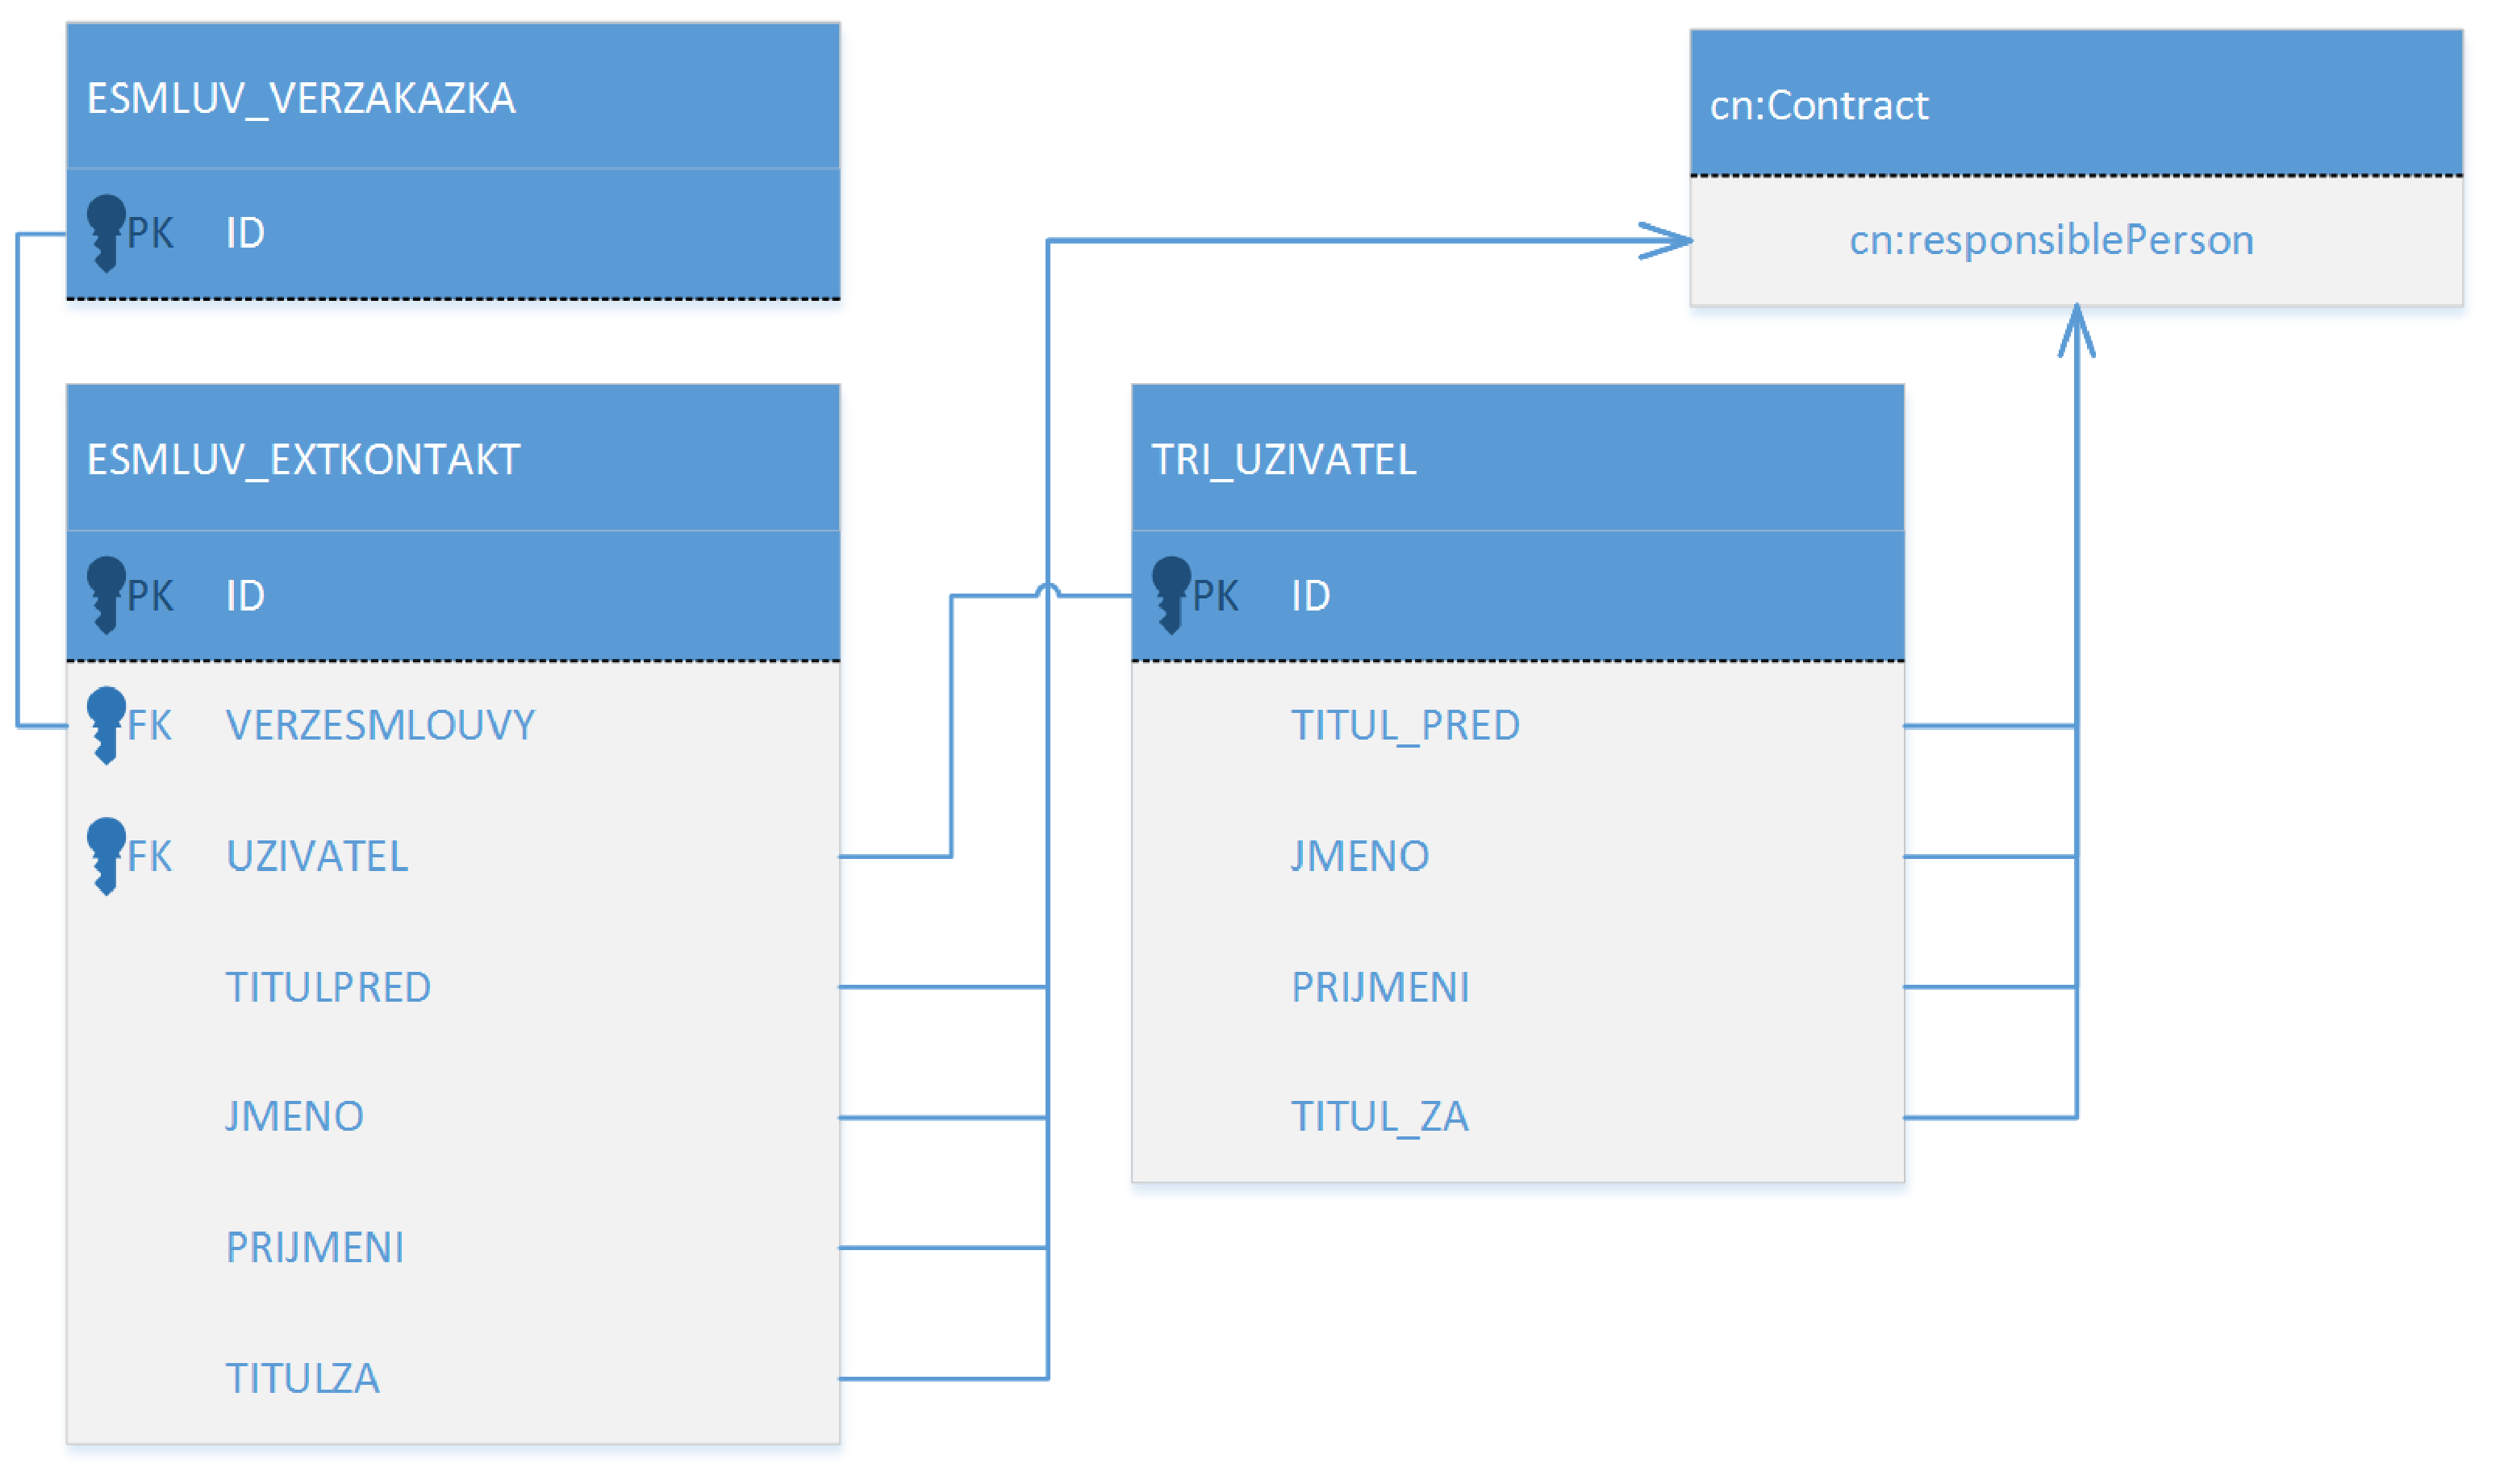
\includegraphics[width=\textwidth]{img/mapRespPerson.eps}}
\caption{R2RML mapování externího kontaktu}
\label{obr:mapRespPerson}
\end{figure}

\subsubsection{Smluvní strana}

Mapování smluvní strany a adresy vychází z údajů tabulek \\ESMLUV\_SMLUVSTRANA a HAD\_POUZITA (viz Obr. \ref{obr:mapParty})

\begin{itemize}
\item \textbf{URI} - \textit{http://[domain]/party/\{HAD\_POUZITA\}}
\item \textbf{Typ} - gr:BusinessEntity
\end{itemize}

\paragraph*{Mapované položky}
\begin{itemize}
\item \textbf{gr:legalName} - Atribut NAZEV\_SUBJEKTU
\item \textbf{dc:identifier} - Atribut ICO
\item \textbf{owl:sameAs} - Atribut ICO, odkaz na reprezentaci ekonomického subjektu v ARESu (LinkedData podoba)
	\begin{itemize}
	\item \textit{http://linked.opendata.cz/resource/business-entity/CZ\{ICO\}}
	\end{itemize}
\item \textbf{cn:noID} - \uv{true} pokud je vyplněno IČ, jinak \uv{false}
\item \textbf{cn:localID} - Atribut HAD\_POUZITA
\item \textbf{schema:addressCountry} - Atribut STAT
\item \textbf{cn:paysVAT} - Atribut PLATCEDPH
\item \textbf{schema:address} - Odkaz na adresu
	\begin{itemize}
	\item \textit{http://[domain]/party/\{HAD\_POUZITA\}/address}
	\end{itemize}
\end{itemize}

\paragraph*{Nenamapované položky}
\begin{itemize}
\item \textbf{cn:payer} - Modul ESML zatím neeviduje kompletní smluvní plnění, takže nelze určit 
\item \textbf{cn:superiorInstitution} - Modul ESML neeviduje nadřazené instituce
\end{itemize}

\subsubsection{Adresa}

\begin{itemize}
\item \textbf{URI} - \textit{http://[domain]/party/{HAD\_POUZITA}/address}
\item \textbf{Typ} - schema:PostalAddress
\end{itemize}

\paragraph*{Mapované položky}
\begin{itemize}
\item \textbf{schema:streetAddres} - Složení atributu ULICE a CISLA
\item \textbf{schema:postalCode} - Atribut PSC
\item \textbf{schema:addressLocality} - Atribut MESTO
\end{itemize}

\paragraph*{Nenamapované položky}
\begin{itemize}
\item \textbf{cn:nuts} - Modul ESML neeviduje hodnoty normalizované klasifikace územních celků
\end{itemize}

\begin{figure}[H]
\centerline{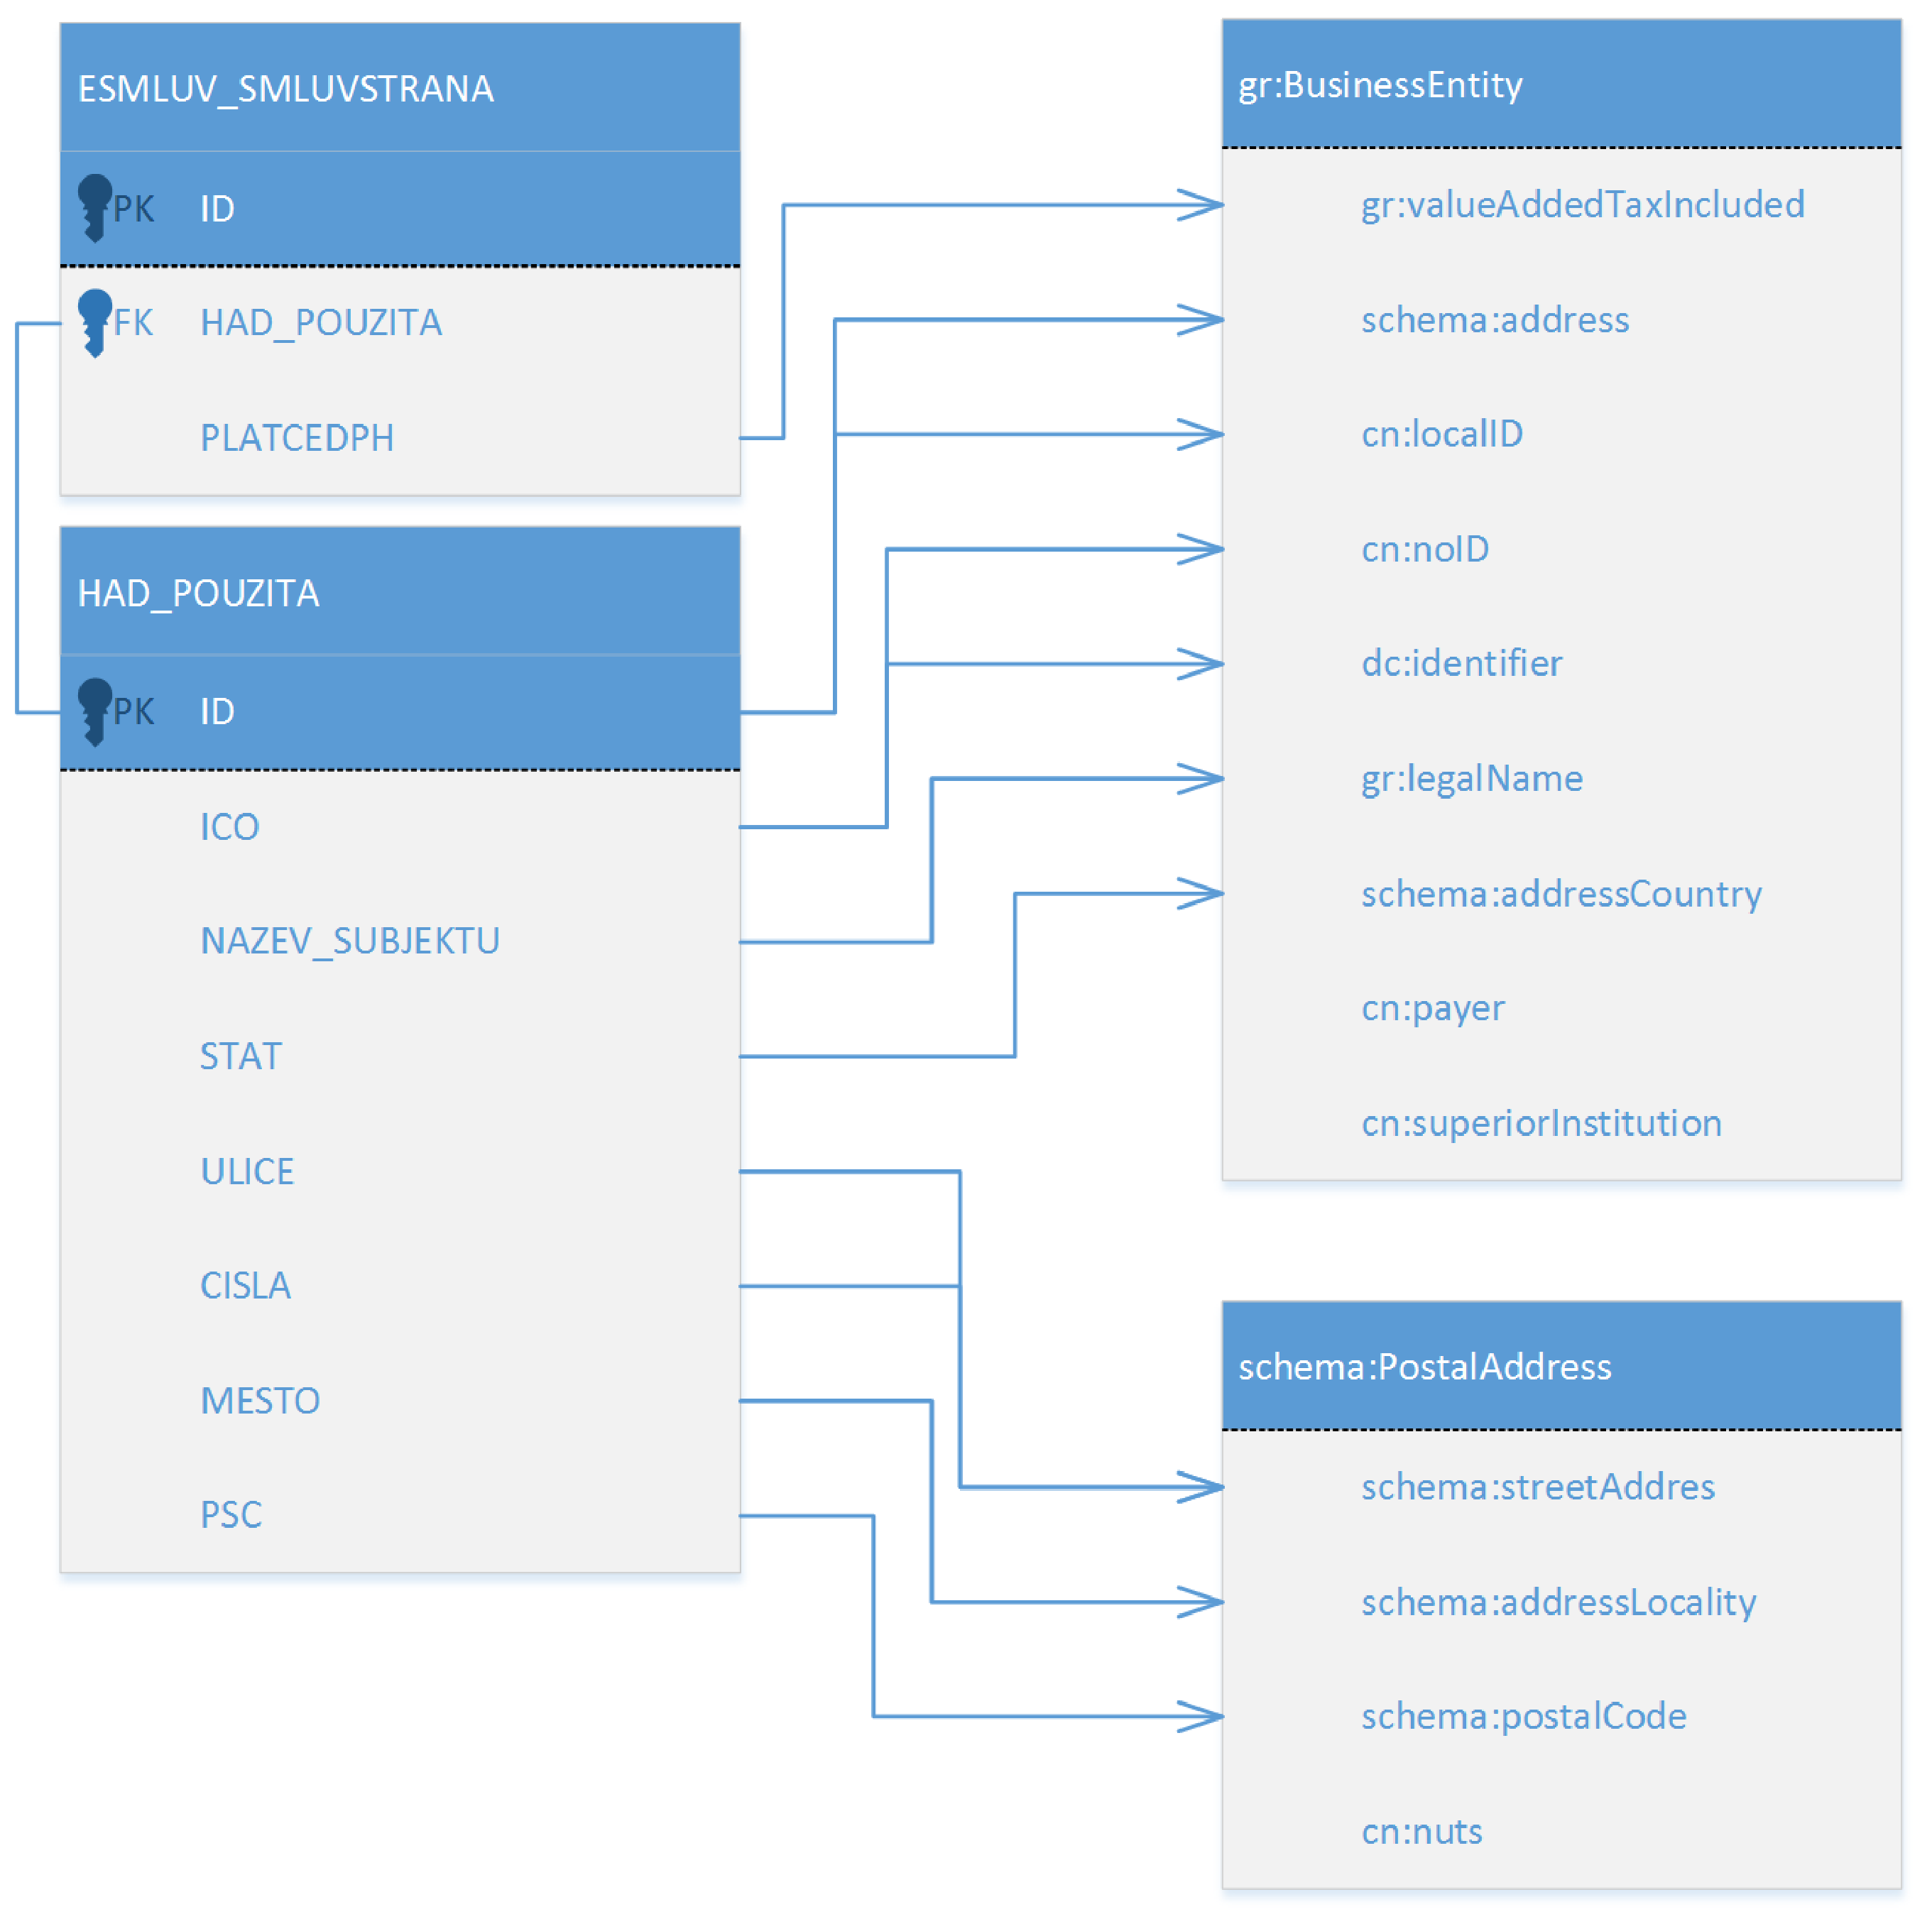
\includegraphics[width=\textwidth]{img/mapParty.eps}}
\caption{R2RML mapování vlastností Smluvní strany a Adresy}
\label{obr:mapParty}
\end{figure}

\subsubsection{Příloha}

Mapování přílohy vychází z údajů tabuly \\ESMLUV\_PRILOHASMLOUVY (viz Obr. \ref{obr:mapAttachment}). V modulu smluv lze přílohy editovat, ale neprovádí se jejich verzování. Proto verze přílohy bude mít vždy hodnotu \uv{1}. Oproti datovému standardu, příloha v datovém modelu Munis ESML popisuje spíše fyzický soubor, nemůžeme tedy namapovat většinu položek entity Dokument, ale jen některé. Nemapované položky proto neuvádíme.

\begin{itemize}
\item \textbf{URI} entity  - \textit{http://[domain]/attachment/\{ID\}/1}
\item \textbf{Typ} - cn:Attachment
\end{itemize}

\paragraph*{Konstanty}
\begin{itemize}
\item \textbf{dcmi:type} - Hodnota \uv{Příloha}
\item \textbf{cn:valid} - Položka je vždy \uv{true}, přílohy nejsou verzované
\end{itemize}

\paragraph*{Mapované položky}
\begin{itemize}
\item \textbf{cn:anonymised} - Atribut ANONYMIZOVANO
\item \textbf{dc:title} - Atribut POPIS\_NAZEV
\item \textbf{dc:identifier} - Atribut ID
\item \textbf{schema:url} - Odkaz na fyzické umístění souboru
	\begin{itemize}
	\item \textit{http://[domain]/file/\{SADADUL\_ULOZISTEID\}/\{NAZEVSOUBORU\}}
	\end{itemize}
\item \textbf{dc:publisher} - Odkaz na vydavatele
	\begin{itemize}
	\item \textit{http://[domain]/publisher}
	\end{itemize}
\item \textbf{cn:version} - Odkaz na informace o verzi smlouvy
	\begin{itemize}
	\item \textit{http://[domain]/attachment/{ID}/1/version}
	\end{itemize}
\item \textbf{cn:contract} - Odkaz na nadřízenou smlouvu. K tomuto údaji je třeba ID Smlouvy (tabulka ESMLUV\_SMLOUVA a pořadí verze smlouvy, tabulka ESMLUV\_VERZESMLOUVY)
	\begin{itemize}
	\item \textit{http://[domain]/attachment/\{ID\}/\{PORADIVERZE\}}
	\end{itemize}
\end{itemize}

\begin{figure}[H]
\centerline{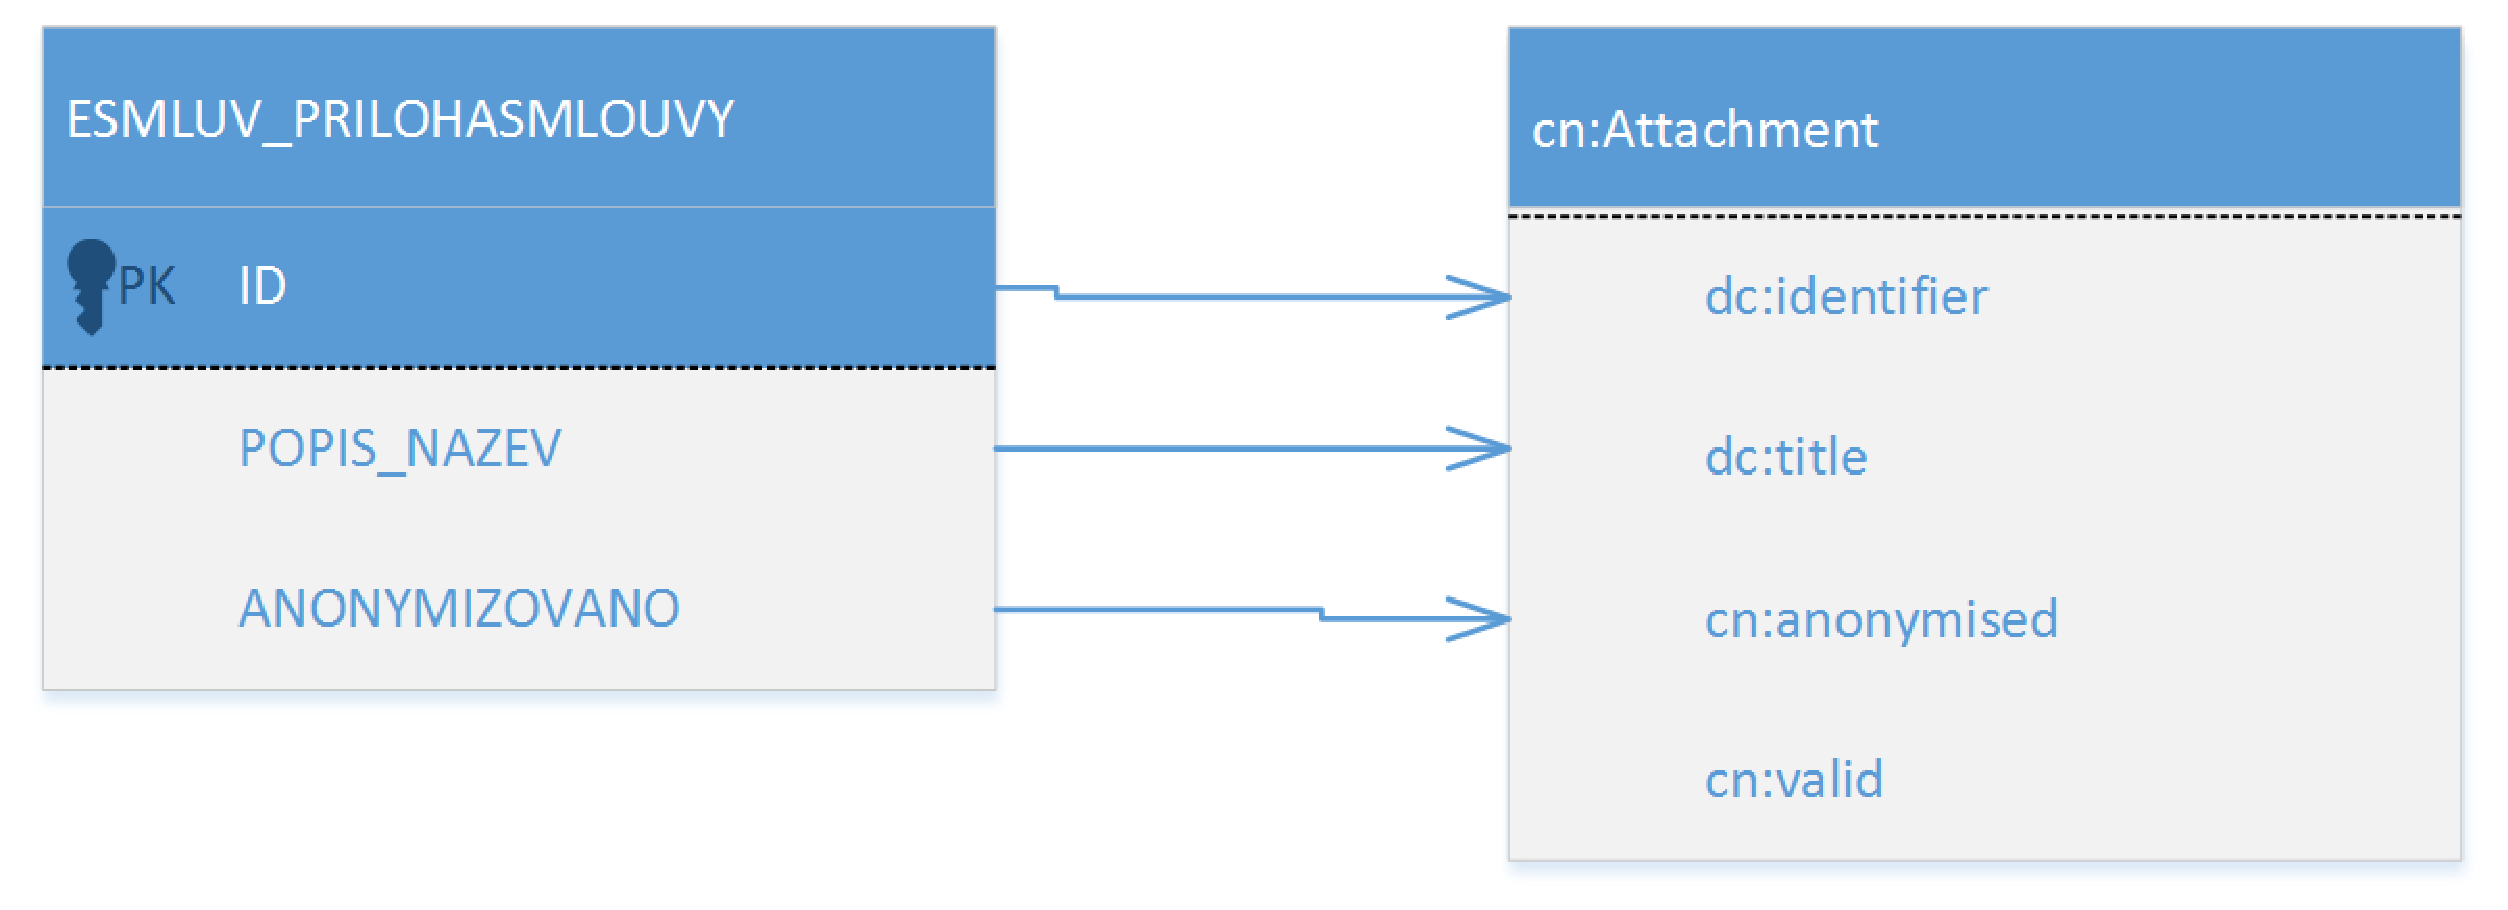
\includegraphics[width=\textwidth]{img/mapAttachment.eps}}
\caption{R2RML mapování vlastností Příloha}
\label{obr:mapAttachment}
\end{figure}

\subsubsection{Dodatek}

Dodatek v datovém modelu Munis ESML je také smlouvou, takže budeme vycházet z atributů jako u smlouvy (viz Obr. \ref{obr:munisSmlouva}).

\begin{itemize}
\item \textbf{URI entity} - \textit{http://[domain]/amendment/{ID}/{PoradiVerzeDodatku}}
\item \textbf{Typ} - cn:Amendment
\end{itemize}

\paragraph*{Konstanty}

\begin{itemize}
\item \textbf{dcmi:type} - s hodnotou \uv{Dodatek}
\end{itemize}

\paragraph*{Mapované položky}

\begin{itemize}
\item \textbf{cn:anonymised} - Atribut ANONYMIZOVANO
\item \textbf{dc:title} - Atribut PREDMET
\item \textbf{dc:identifier} - Atribut ID
\item \textbf{dc:created} - Atribut DATUMPODPISU
\item \textbf{cn:valid} - Položka je \uv{true}, jestliže se jedná o nejnovější verzi dodatku, jinak je \uv{false}
\item \textbf{cn:contract} - Odkaz rodičovskou smlouvu
	\begin{itemize}
	\item \textit{http://[domain]/contract/\{RODIC\}/\{PORADIVERZE\}}
	\end{itemize}
\item \textbf{dc:publisher} - Odkaz na vydavatele
	\begin{itemize}
	\item \textit{http://[domain]/publisher}
	\end{itemize}
\item \textbf{cn:version} - Odkaz na informace o verzi dodatku
	\begin{itemize}
	\item \textit{http://[domain]/contract/\{ID\}/\{PORADIVERZE\}/version}
	\end{itemize}
\item \textbf{schema:url} - Odkaz na fyzický dokument dodatku
	\begin{itemize}
	\item \textit{http://[domain]/file/\{SADADUL\_ULOZISTEID\}/\{NAZEVSOUBORU\}}
	\end{itemize}
\item \textbf{cn:responsiblePerson} - Každá veřejná zakázka má vazbu na externí kontakty. Externím kontaktem může být buď uživatel informačního systému (tabulka TRI\_UZIVATEL), nebo jakákoli osoba vyplněná v tabulce Externí kontakt. Pro potřeby mapování se hodnoty spojí do jednoho řetězce, viz Obr. \ref{obr:mapRespPerson}.
\end{itemize}

\paragraph*{Nenamapované položky}
\begin{itemize}
\item \textbf{cn:uri} - Položka odpovídá URI entity
\item \textbf{cn:plainText} - Prostý text dokumentu smlouvy, resp. alternativa k oskenovaným dokumentům. Vyžaduje hlubší analýzu procesu zpracování dokumentů 
\end{itemize}

\subsubsection{Verze dokumentu}

K mapování jednotlivých verzí smlouvy/přílohy/dodatku. Pro smlouvy/dodatky mapujeme z tabulky ESMLUV\_VERZESMLOUVY (viz Obr. \ref{obr:mapVersion}). Pro přílohu mapujeme z tabulky ESMLUV\_PRILOHA (viz. Obr. \ref{obr:mapAttachment})

\begin{itemize}
\item \textbf{URI entity}
	\begin{itemize}
	\item U smlouvy/dodatku - \\\textit{http://[domain]/[type]/\{ID\}/\{PORADIVERZE\}/version}
	\item U přílohy - \textit{http://[domain]/attachment/\{ID\}/1/version}
	\end{itemize}
\item \textbf{Typ} - cn:Version
\end{itemize}

\paragraph*{Mapované položky}
\begin{itemize}
\item \textbf{cn:uri} - Položka je stejná jako URI entity
\item \textbf{cn:versionOrder} - U smlouvy/dodatku atribut PORADIVERZE, u přílohy hodnota \uv{1}
\item \textbf{dc:issued} - U smlouvy/dodatku atribut DATUMZMENYSTAVU\_TS, u přílohy hodnota OKAMZIKVYTVORENI
\end{itemize}

\paragraph*{Nenamapované položky}
\begin{itemize}
\item \textbf{cn:publisherId} - Díky Id a verzi dokumentu máme každou entitu jednoznačně identifikovanou, proto není třeba vyplňovat.
\end{itemize}

\begin{figure}[H]
\centerline{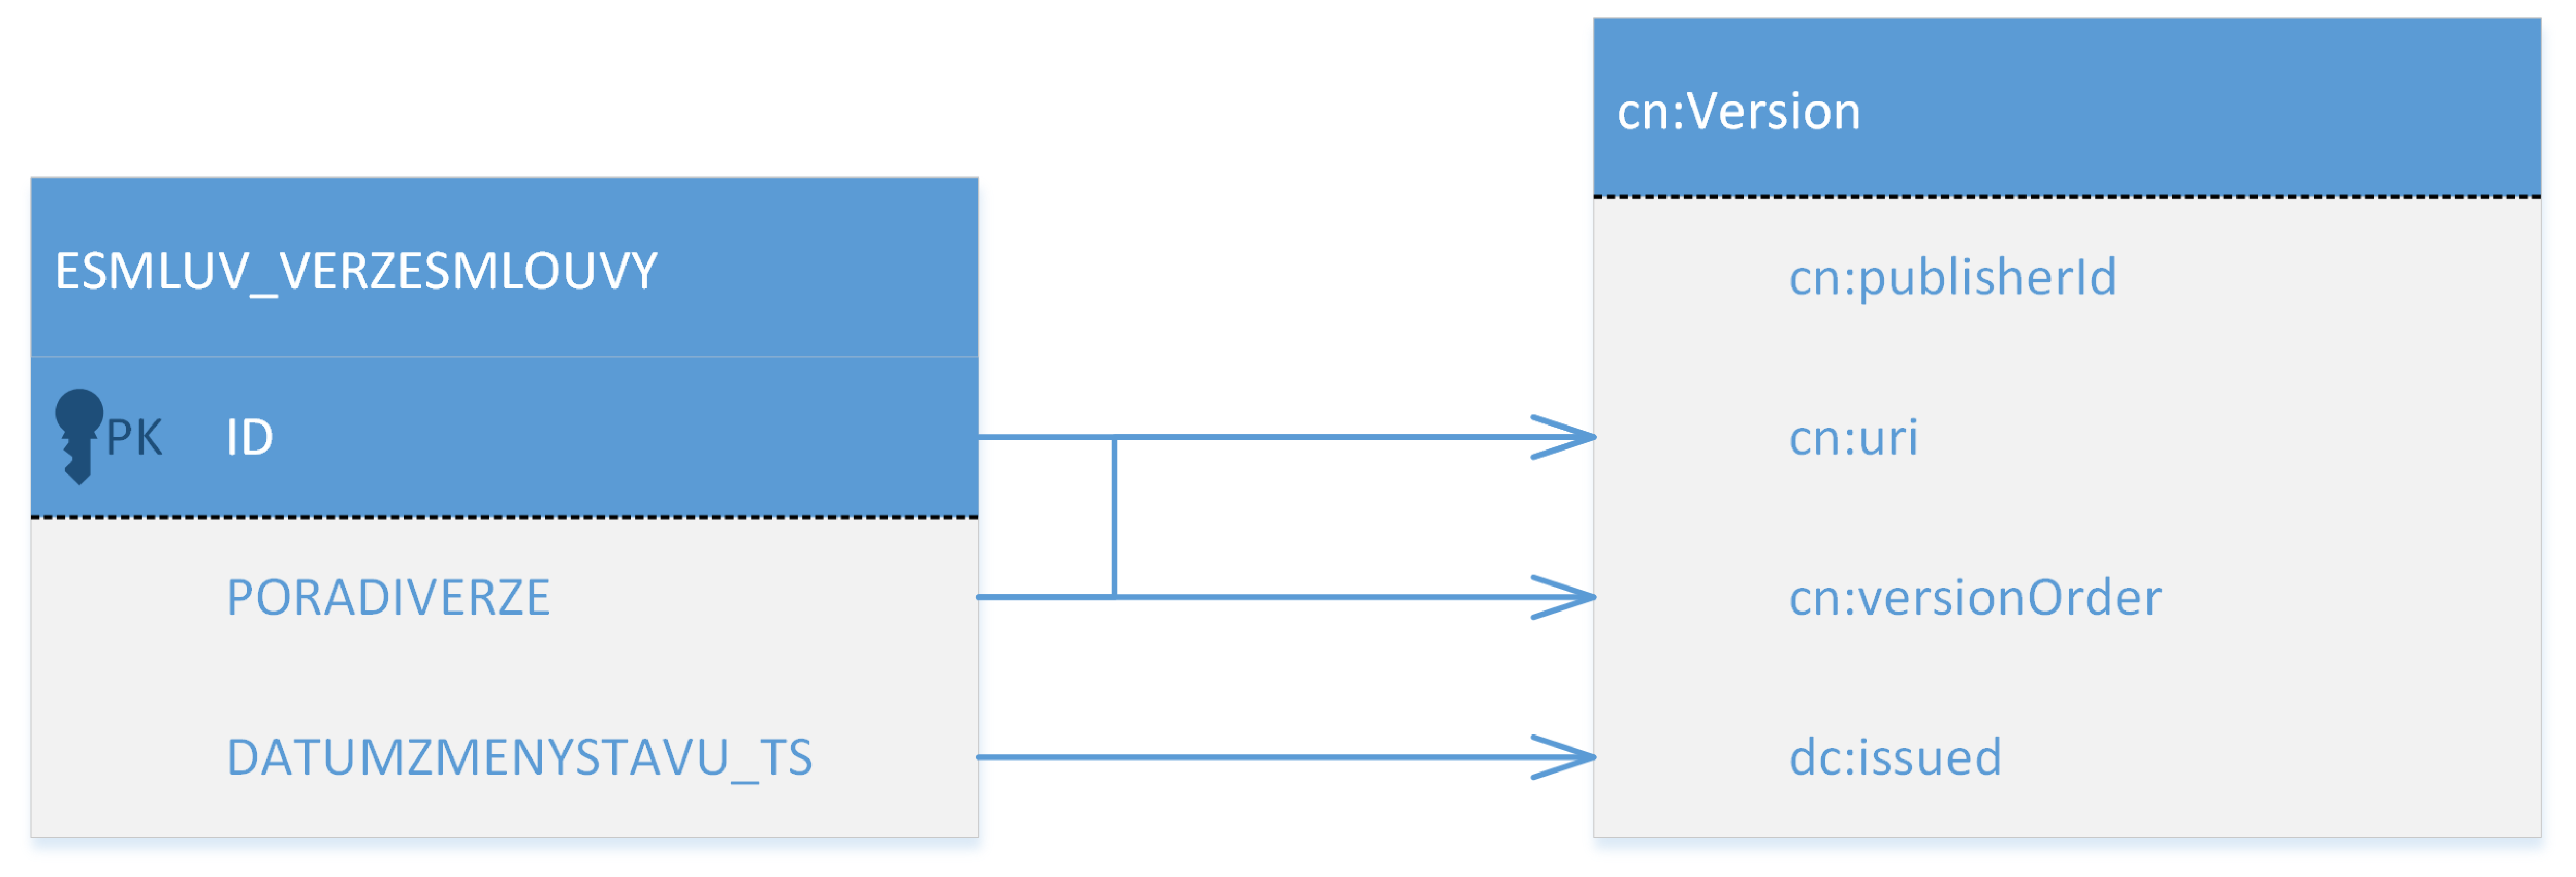
\includegraphics[width=\textwidth]{img/mapVersion.eps}}
\caption{R2RML mapování vlastností Verze}
\label{obr:mapVersion}
\end{figure}

\subsubsection{Implementace}

Entitu implementace nereprezentuje žádná tabulka v rámci datového modulu ERMS. Je třeba ji proto vytvořit s odpovídajícími položkami. Využijeme tabulek ESMLUV\_SMLOUVA, ESMLUV\_VERZESMLOUVY a ESMLUV\_MILNIK. 

\begin{itemize}
\item \textbf{URI entity} - \textit{http://[domain]/contract/{ID}/{PORADIVERZE}/implementation}
\item \textbf{Typ} - cn:Implementation
\end{itemize}

\paragraph*{Mapované položky}
\begin{itemize}
\item \textbf{cn:milestone} - Položka je stejná jako URI entity
	\begin{itemize}
	\item textit{http://[domain]/contract/\{ID\}/\{PORADIVERZE\}/milestone/- \{MilestoneID\}}
	\end{itemize}
\end{itemize}

\subsubsection{Milník}

K mapování milníků využijeme tabulek ESMLUV\_SMLOUVA, \\ESMLUV\_VERZESMLOUVY a ESMLUV\_MILNIK (tabulka milníku viz Obr. \ref{obr:mapMilestone}).

\begin{itemize}
\item \textbf{URI entity} - \textit{http://[domain]/contract/\{ID\}/\{PORADIVERZE\}/milestone/-
\{MilestoneID\}}
\item \textbf{Typ} - cn:Milestone
\end{itemize}

\paragraph*{Mapované položky}
\begin{itemize}
\item \textbf{dc:title} - Atribut NAZEV
\item \textbf{cn:dueDate} - Atribut DATUMUCINOSTIML
\end{itemize}

\begin{figure}[H]
\centerline{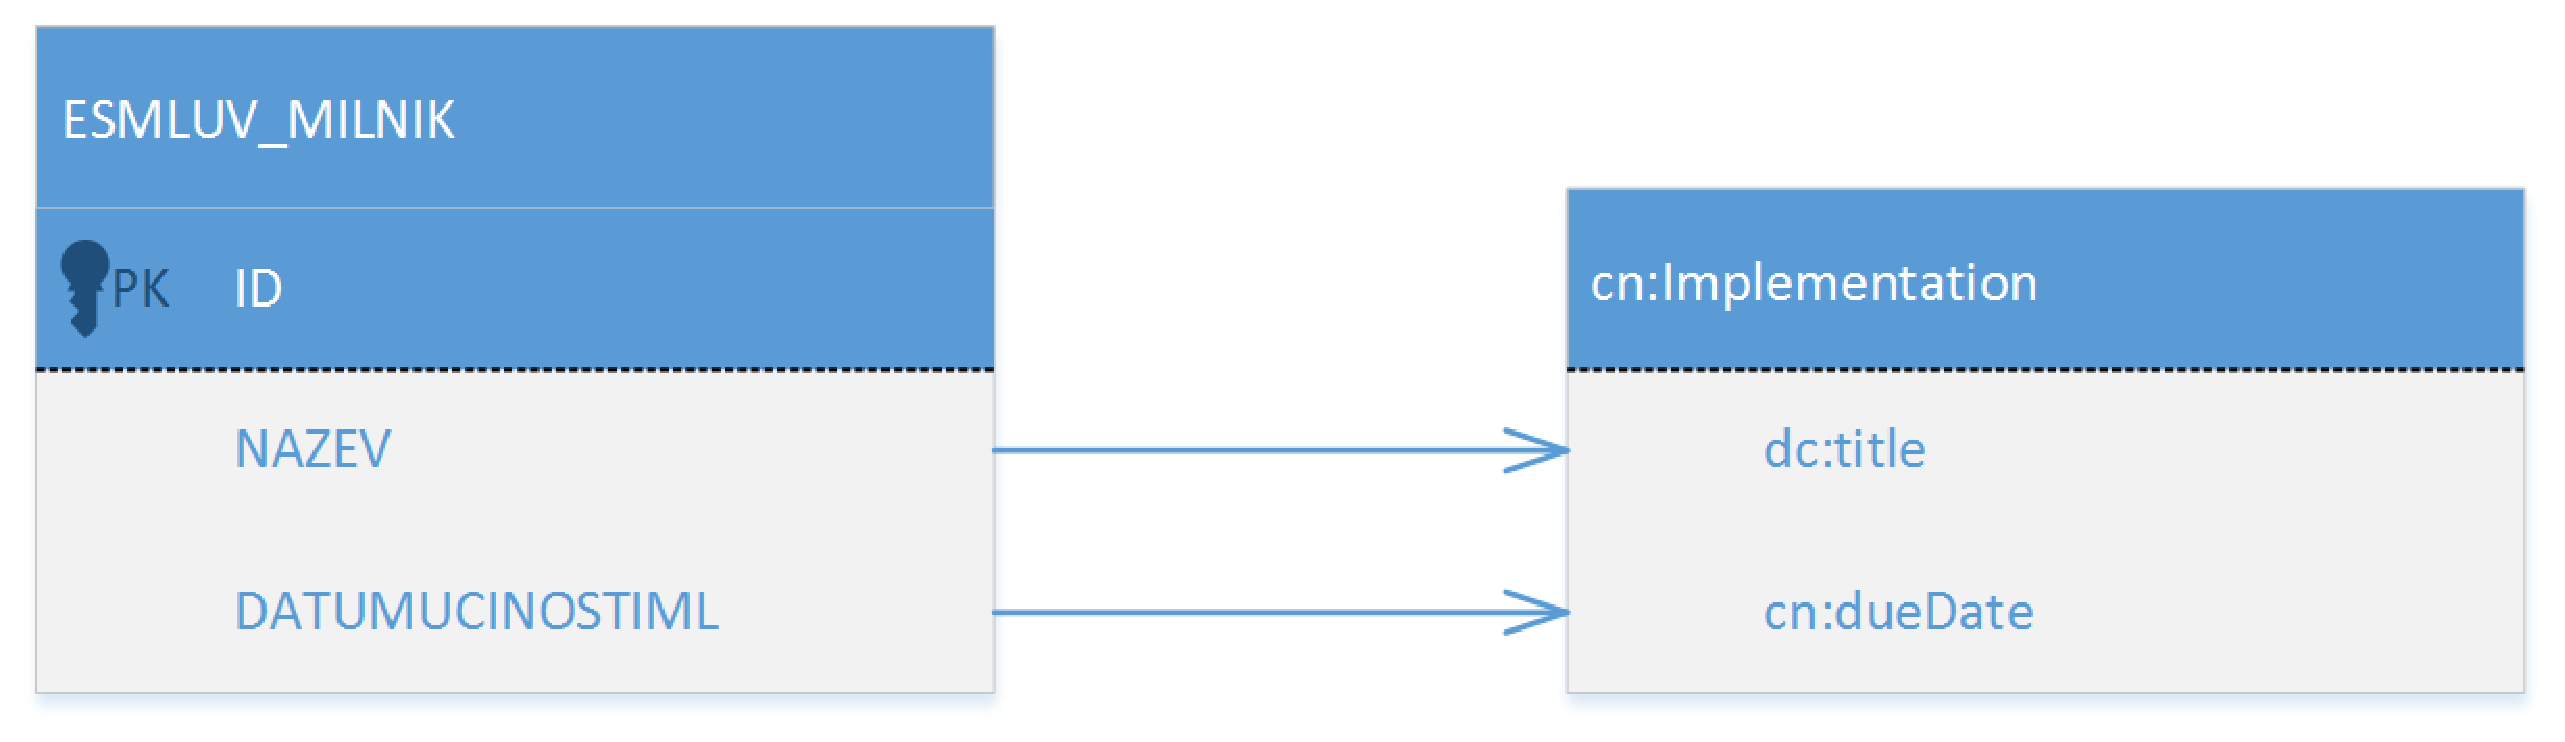
\includegraphics[width=\textwidth]{img/mapMilestone.eps}}
\caption{R2RML mapování vlastností Milníku}
\label{obr:mapMilestone}
\end{figure}

\subsubsection{Vydavatel}

Vydavatele namapujeme pomocí tabulky TRI\_ORGADR, viz Obr. \ref{obr:mapPublisher}

\begin{itemize}
\item \textbf{URI entity}  - \textit{http://[domain]/publisher}
\item \textbf{Typ} - foaf:Organization
\end{itemize}

\paragraph*{Konstanty}
\begin{itemize}
\item \textbf{schema:addressCountry} - Hodnota \uv{CZE}
\end{itemize}

\paragraph*{Mapované položky}
\begin{itemize}
\item \textbf{gr:legalName} - Atribut NAZEVORGANIZACE
\item \textbf{cn:noID} - \uv{true} pokud je vyplněno IČ, jinak \uv{false}
\item \textbf{dc:identifier} - Atribut ICO
\item \textbf{owl:sameAs} - Atribut ICO, odkaz na reprezentaci ekonomického subjektu v ARESu (LinkedData podoba)
	\begin{itemize}
	\item \textit{http://linked.opendata.cz/resource/business-entity/CZ\{ICO\}}
	\end{itemize}
\end{itemize}

\paragraph*{Nenamapované položky}
\begin{itemize}
\item \textbf{cn:authentication} - Pro naše účely nemá smysl
\end{itemize}

\begin{figure}[H]
\centerline{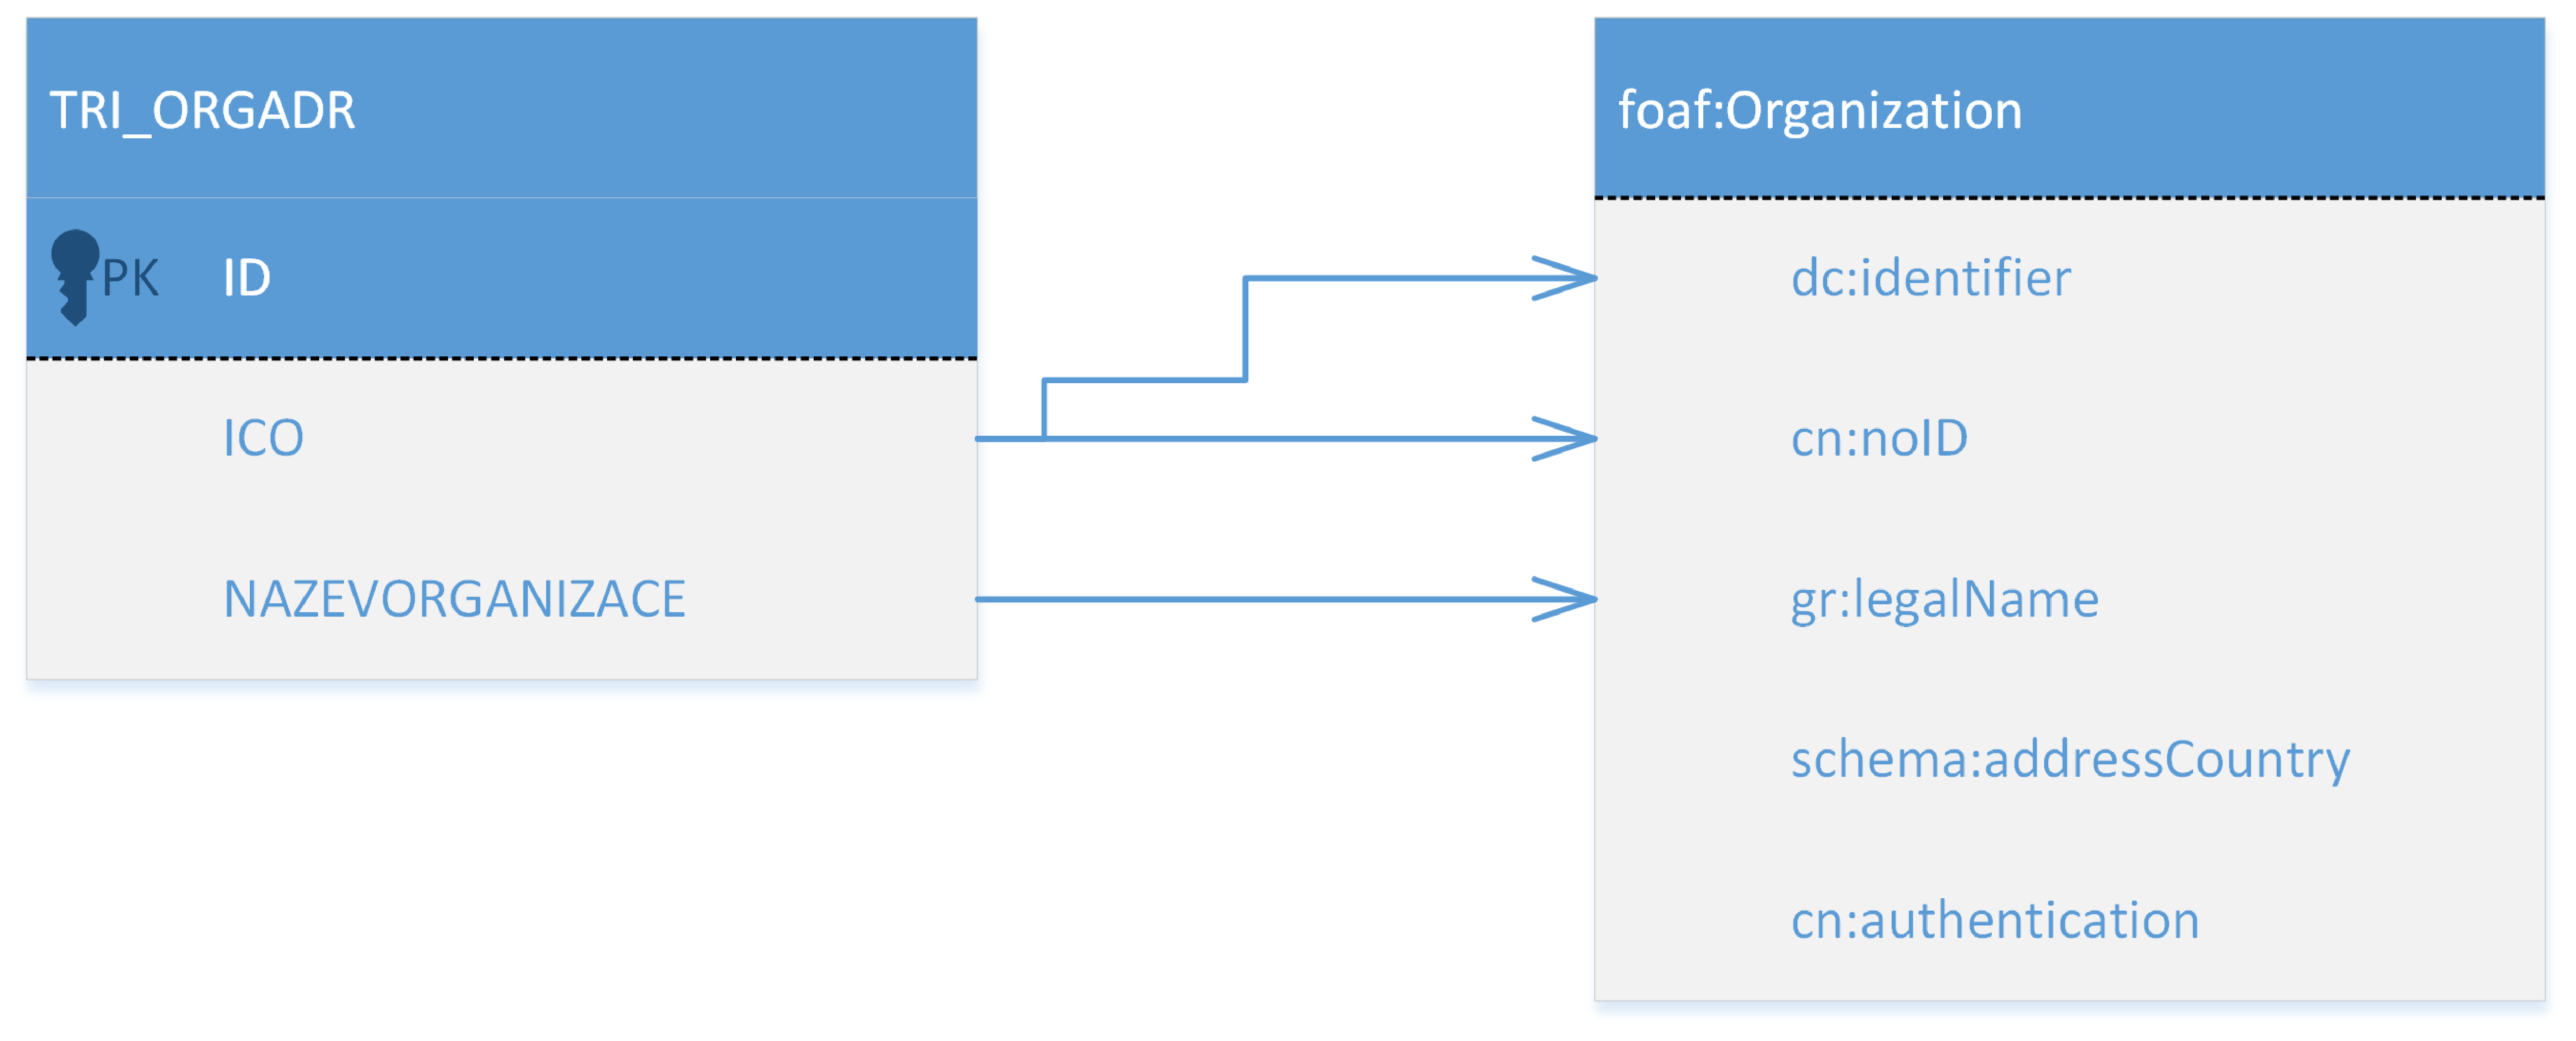
\includegraphics[width=\textwidth]{img/mapPublisher.eps}}
\caption{R2RML mapování vlastností Vydavatele}
\label{obr:mapPublisher}
\end{figure}

\subsection{Volba technologií a implementační platformy}

Pro samotnou implementaci konverzního mechanismu zvolíme platformu .Net. Modul bude mít formu webové aplikace, resp. virtuálního SPARQL endpointu, kterou budeme implementovat v technologii ASP.Net. Využijeme tradičního architektonického vzoru MVC. K práci s RDF daty budeme využívat knihovnu dotnetRdf.

\subsubsection{Volba R2RML procesoru}

K R2RML mapování využijeme projektu DotNetR2RMLStore\cite{r2rmlstore}\cite{r2rmlproj}. Jedná se o experimentální R2RML procesor pracující nad relačními databázemi Microsoft SQL\footnote{Většina veřejných institucí využívající produkty firmy Triada. spol, s.r.o. pracuje nad databázemi MS SQL. Proto nebereme MS SQL jako omezení. Munis ESML ale umožňuje práci i nad databází Oracle.}. Tento projekt je vytvářený v rámci Katedry softwarového inženýrství na Matematicko-fyzikální fakultě. 

\subsubsection*{Omezení R2RML procesoru}

Využití zmíněného R2RML procesoru si vyžádalo několik drobných omezení. 

Pro náš případ využijeme DotNetR2RMLStore ve verzi 0.0.0.9. Zkoušená vyšší verze mění logiku zpracování dotazů a zatím nepodporuje SQL Views. Je tu i možnost vytvořit SQL views přímo nad databází subjektu a mapovat R2RML skriptem přímo tyto pohledy. Není to problém, ale nelze považovat za samozřejmost, že subjekt zpřístupní databázi k úpravám. 

Procesor nepodporuje SPARQL příkazy ASK a DESCRIBE. Pro naše účely ale stačí hlavní příkazy SELECT a CONSTRUCT.

Samotný R2RML skript musí mít v hodnotě \textit{template} vždy vyplněné absolutní URI. Prefixovaný zápis procesor zpracuje, ale při zpracovaní dotazů daný template nerozpozná.

Formáty datumových položek v RDF datech by měly splňovat W3C specifikaci, což aktuálně nesplňují. Vrácené datumové hodnoty tedy v rámci postprocesingu nahradíme správným formátem\cite{datetime}. 

\subsubsection{Napojení na datové úložiště}

Mezi specifika informačních systémů firmy Triada s.r.o můžeme zmínit, že neukládají fyzické soubory (v našem případě smlouvy) do databáze s ostatními daty, ale do specializovaného datového úložiště. Nutnou podmínkou pro zobrazení těchto dat je proto propojení konverzního modulu s databází datového úložiště. Využijeme k tomu knihovnu TriadaModulZaklad.

V relační databázi jsou uloženy informace o daném souboru. Jedná se mimo jiné o název souboru a jeho jednoznačný indentifikátor v datovém úložišti ve formě GUID. Informace tedy namapujeme již na zmíněné URI -\\\textit{http://[domain]/file/{SADADUL\_ULOZISTEID}/{NAZEVSOUBORU}}. Při přístupu na danou adresu se informace převedou na dotaz do datového úložiště a uživateli se vrátí konkrétní soubor ke stažení.

\subsection{SPARQL endpoint}

Virtuální SPARQL endpoint vystavený nad konverzním modulem je dostupný na adrese:

\begin{itemize}
\item \textit{http://[domain]/sparql}
\end{itemize}

Interface endpointu se skládá z jednoduchého pohledu obsahující formulář pro zadávání SPARQL dotazů a volbu požadovaného výstupního formátu. Každý zadaný SPARQL dotaz je enkódován jako HTTP Get na základě kterého pak modul vrátí požadovaná data. Obdobně také probíhá dereferencování entit. Zadané HTTP URI reprezentující konkrétní entitu se převede na odpovídající SPARQL příkaz CONSTRUCT. Výsledný dotaz pak vypadá takto:

\begin{itemize}
\item \textit{http://[domain]/sparql?query=\{SPARQLQUERY\}\&Format=\{OUTPUT\}}
\item SPARQLQUERY značí SPARQL dotaz 
\item OUTPUT reprezentuje požadovaný výstupní formát\footnote{U derefencovaných entit je vždy výstupní formátem HTML. Je to z důvodu možnosti prohlížení a listování mezi entitami pomocí hypertextových odkazů, viz Zpracování RDF výstupu.}. Defaulntí hodnotou je formát HTML.
\end{itemize}

Možnost DUMPu dat v podstatě znamená příkaz CONSTRUCT nad všemi daty. Má však speciální konstrukci:

\begin{itemize}
\item \textit{http://[domain]/dump?Format=\{OUTPUT\}\&Store=\{STORE\}}
\item OUTPUT reprezentuje požadovaný výstupní formát
\item STORE nabývá buď hodnoty InMemory (zpracování v paměti), nebo Stream (proudové zpracování). Defaultní hodnotou je InMemory. 
\end{itemize}

\subsection{Zpracování RDF výstupu}

Příkazy SELECT jsou zpracovávány proudově v tabulkové formě, resp. seznamem definovaných proměnných a výčtem hodnot, které jim odpovídají. Definujeme proto handler naslouchající nad R2RML procesorem, kterým výsledky dotazu postupně zpracováváme. Pro každý výstupní formát proto implementujeme handler serializující výsledky do zvoleného datového formátu. Aplikace podporuje základní formáty jako HTML, Turtle, N-Triples, RDF/XML, XML, JSON a CSV. Formáty XML, JSON, CSV serializujeme jako SPARQLResults podle doporučení W3C\cite{Sparqlresults}.

Výhodou proudového přístupu je možnost zpracování teoreticky neomezeného množství dat s dobou zpracování lineárně závisející na daném vstupu.

Příkazem CONSTRUCT získáme na výstupu RDF graf ve formě trojic. Dotaz můžeme zpracovávat jak proudově, tak v paměti. Nevýhodou proudového zpracování je, že nám výsledky přicházejí postupně, data proto lze jen obtížně zkracovat pomocí prefixů, sdružovat související informace apod. V druhém případě máme výsledek uložený v interní reprezentaci jako RDF graf. Graf tedy můžeme procházet a formátovat libovolným způsobem. Nevýhodou jsou vysoké paměťové nároky. Aplikace v obou případech podporuje serializaci do formátů HTML, Turtle, N-Triples, RDF/XML, XML, JSON a CSV. Výstup HTML také slouží k prohlížení dat. Jednotlivé URI jsou ve formě hypertextových odkazů, lze tedy procházet mezi provázanými entitami.

\subsubsection*{Zpracování JSON-LD}

Zvláštní kapitolou je formát JSON-LD. Tento formát není určen pro dotazování, ale spíše na zpracování výsledného grafu. Zavedeme ho tedy jako další možnost zpracování DUMPu dat. Ke zpracování RDF dat potřebujeme načíst definovaný JSON-LD Context, provést mapování nad RDF daty a následně strukturu upravit tak, aby byla validní vůči JSON schématu datového standardu. K mapování využijeme knihovnu JSON-LD.Net. Knihovna však nereflektuje JSON datové typy, resp. všechny hodnotové typy jsou String. Výsledek by tak nebyl validní vůči JSON schématu. Lehce tedy knihovnu upravíme, aby vracela požadované datové typy (viz kód \ref{lst:jsonld_exntension}).

\lstinputlisting[label=lst:jsonld_exntension, caption=Rozšíření knihovny JSON-LD.Net
, language=C++]{code/jsonld_exntension.cs}

\subsection{Konfigurace}

Veškeré důležité nastavení aplikace se nachází v souboru \textit{Web.config}, převážně:

\begin{itemize}
\item Natavení \textit{ConnectionStringu} k relační databázi
\item Nastavení přístupových údajů k datovému úložišti firmy Triada s.r.o
\end{itemize}

Samotný R2RML mapovací skript je umístěn ve složce \textit{App\_Data} v kořenové větvi projektu.

\subsection{Požadavky na architekturu}

R2RML procesor zajišťuje komunikaci s databází a samotný převod relačních dat do RDF. Z architektonického pohledu tedy reprezentuje databázový a zároveň i převodní modul. Kapitoly SPARQL endpoint a Zpracování RDF výstupu reprezentují Publikační modul architektury. Konečně, kapitola Konfigurace odpovídá konfiguračnímu modulu.

\section{Jednotné úložiště}

K sběru a zpracování dat využijeme nástroje Unified views. Jedná se o nástroj na jehož vývoji spolupracuje katedra softwarového inženýrství na MFF UK v rámci evropského projektu LOD2\cite{lod2}.

\subsection{Nástroj Unified views}

Nástroj Unified views funguje na bázi zřetězeného zpracování (Pipelining) propojených funkčních jednotek (DPU - Data processing unit). Naším úkolem je vytvořit takovou pipeline, aby se postupně provedly následující kroky:

\begin{itemize}
\item Načtení a zpracování definovaného datového katalogu s datasety subjektů
\item Stažení jednotlivých datasetů a případně provedení operací související s možnou heterogenitou dat
\item Uložení předzpracovaných dat do triplestore databáze
\item Zpřístupnění dat skrze SPARQL endpoint a registrování datové sady v datovém katalogu
\end{itemize}

Výsledná pipeline je vidět na Obr. \ref{obr:unv}. Proces zpracování pipeline probíhá po směru šipek. 

\begin{figure}[H]
\centerline{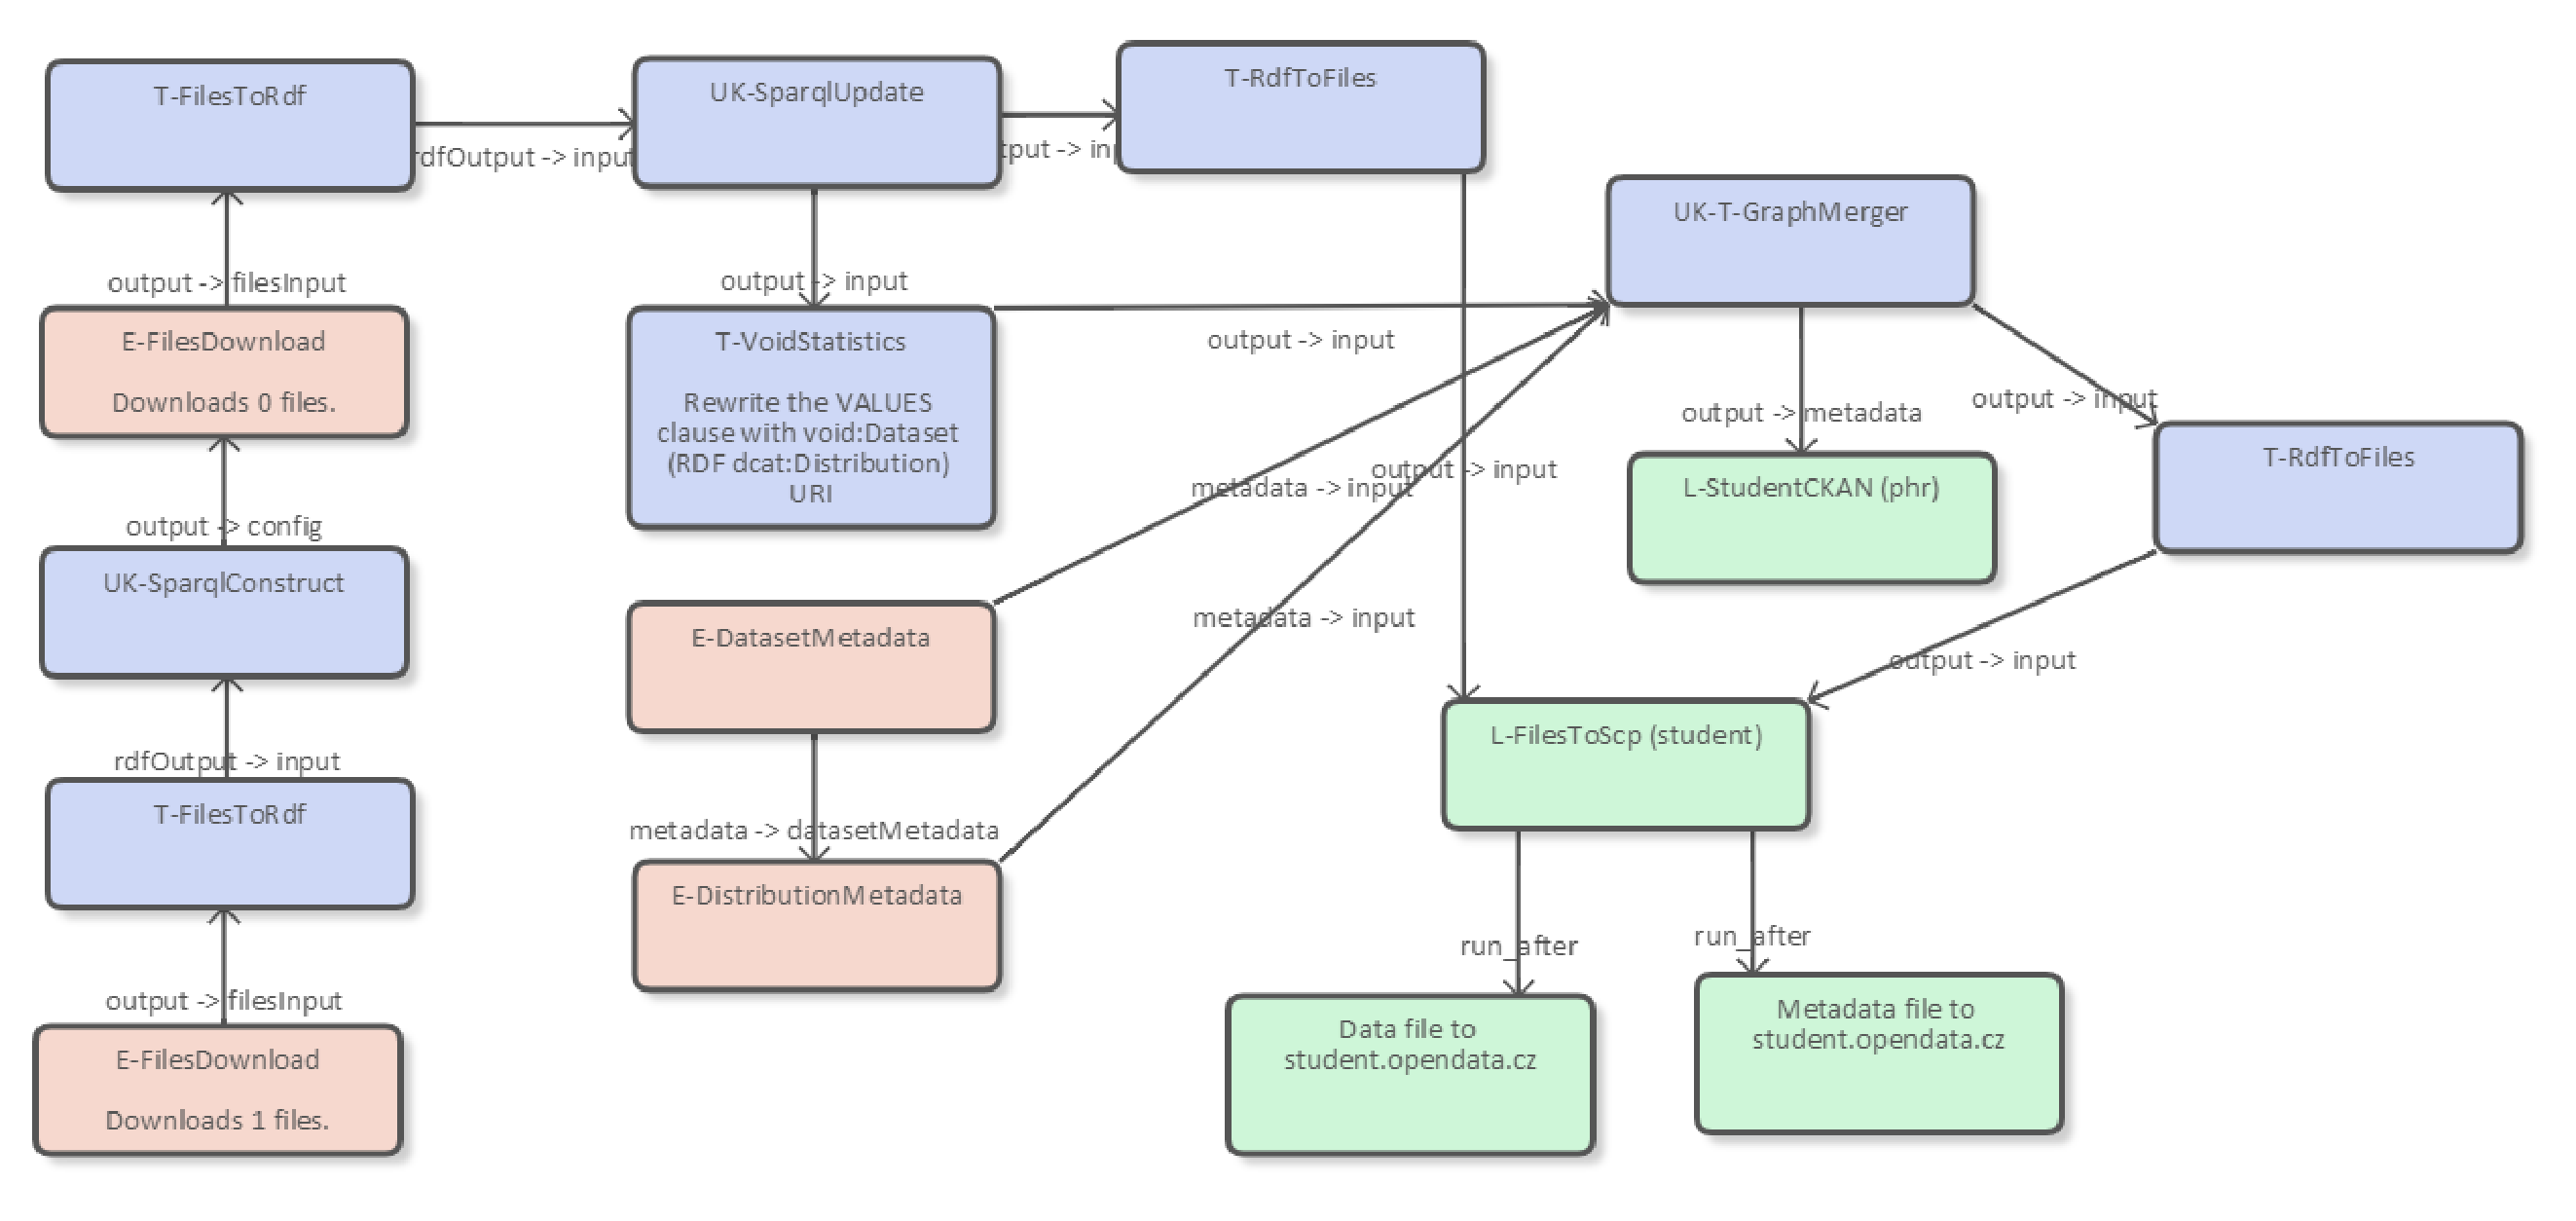
\includegraphics[width=\textwidth]{img/unv.eps}}
\caption{Pipeline nad jednotným úložištěm pro zpracování dat o smlouvách}
\label{obr:unv}
\end{figure}

\subsubsection*{Načtení datového katalogu}

K načtení, resp. zpracování datového katalogu s datasety subjektů slouží první tři DPU pipeliny (viz Obr. \ref{obr:unv} vlevo dole). V rámci prvního DPU - E-FilesDonwload načteme požadovaný datový katalog \ref{lst:subject_catalog}. V druhém DPU - T-FilesToRdf převedeme načtená data do RDF reprezentace. Pokud však chceme pomocí nástroje Unified views dávkově stahovat data, je nutné, aby splňovaly strukturu znázorněnou příkladem kódu \ref{lst:unvConfigurationSample}. Vytvoříme tedy SPARQL příkaz mapující informace z původního datového katalogu do požadované reprezentace (viz Kód \ref{lst:unvLoadCatalog}). Pro tuto funkcionalitu využijeme DPU - UK-SparqlContruct.

\lstinputlisting[label=lst:unvConfigurationSample, caption=Příklad formátu dat pro dávkové zpracování nástrojem UV, language=XML]{code/unvConfigurationSample.ttl}

\lstinputlisting[label=lst:unvLoadCatalog, caption=Příkaz mapující datový katalog do reprezentace nástroje UV, language=XML]{code/unvLoadCatalog.sparql}

\subsubsection*{Zpracování jednotlivých datasetů}

Nyní pomocí DPU - E-FilesDonwload již můžeme stáhnout požadované datasety a pomocí DPU - T-FilesToRdf je převést do RDF reprezentace. V rámci předzpracování provedeme nad daty tuto operaci (v rámci DPU - UK-SparqlUpdate):

\begin{itemize}
\item Obecně subjekt publikující smlouvy nutně nemusí mít podrobné informace o smluvních stranách, ale např. má jen IČ. Za předpokladu, že u smluvních stran je vyplněno jen IČ, tak vytvoříme propojení na odpovídající objekt v Linked Data reprezentaci ekonomického subjektu (Viz Kód\ref{lst:unvPreprocesing}).  
\end{itemize}

\lstinputlisting[label=lst:unvPreprocesing, caption=Příkaz mapující IČ na reprezentaci ekonomického subjektu, language=XML]{code/unvPreprocesing.sparql}

\subsubsection*{Uložení a publikace výsledné datové sady}

V první fázi definujeme Metadata o celé datové sadě reprezentující smlouvy. Popíšeme, k čemu datová sada slouží, jaké má URI, licence apod. K tomu slouží DPU - E-DatasetMetadata a DPU - E-DistributionMetadata. Nad datasetem provedeme také statistické výpočty (počty trojic, entit, tříd atd.) pomocí SPARQL příkazu \ref{lst:unStats} v rámci DPU - T-VoidStatistics. 

\lstinputlisting[label=lst:unStats, caption=Statistické výpočty nad Otevřenými smlouvami, language=XML]{code/unStats.sparql}

V druhé fázi výsledky z těchto DPU slijeme dohromady pomocí DPU - UK-T-GraphMerger. Tímto nám vzniknou úplná metadata o datové sadě otevřených smluv. Tyto informace již můžeme zveřejnit v rejstříku datových sad. V našem případě nad platformou CKAN\cite{ckan} (pomocí DPU - L-StudentCKAN). Datová sada je dostupná na adrese:

\begin{itemize}
\item \textit{http://student.opendata.cz/dataset/phr-contracts }\cite{contractCkan}
\end{itemize}

V poslední, třetí fázi data i metadata serializujeme do výstupních souborů v RDF formátu (obě DPU - T-RdfToFiles) a publikujeme do triplestore databáze Virtuoso Universal Server\cite{virtuoso} (Zbylé DPUs). Vystavený sparql endpoint je dostupný na adrese

\begin{itemize}
\item \textit{http://student.opendata.cz/sparql}
\end{itemize}

\subsection{Požadavky na architekturu}

Databázovým, převodním i publikačním modulem je v našem případě nástroj Unified views. Konfigurací rozumíme jednak nastavení jednotlivých DPU v rámci pipeline, tak načítaný soubor s katalogem požadovaných datových sad. Posledním požadavkem je možnost nastavení intervalu exekuce definované pipeline. V rámci nástroje Unified views k tomu slouží funkce \uv{Schedule a pipeline} (viz Obr. \ref{obr:unvSchedule}).

\begin{figure}[H]
\centerline{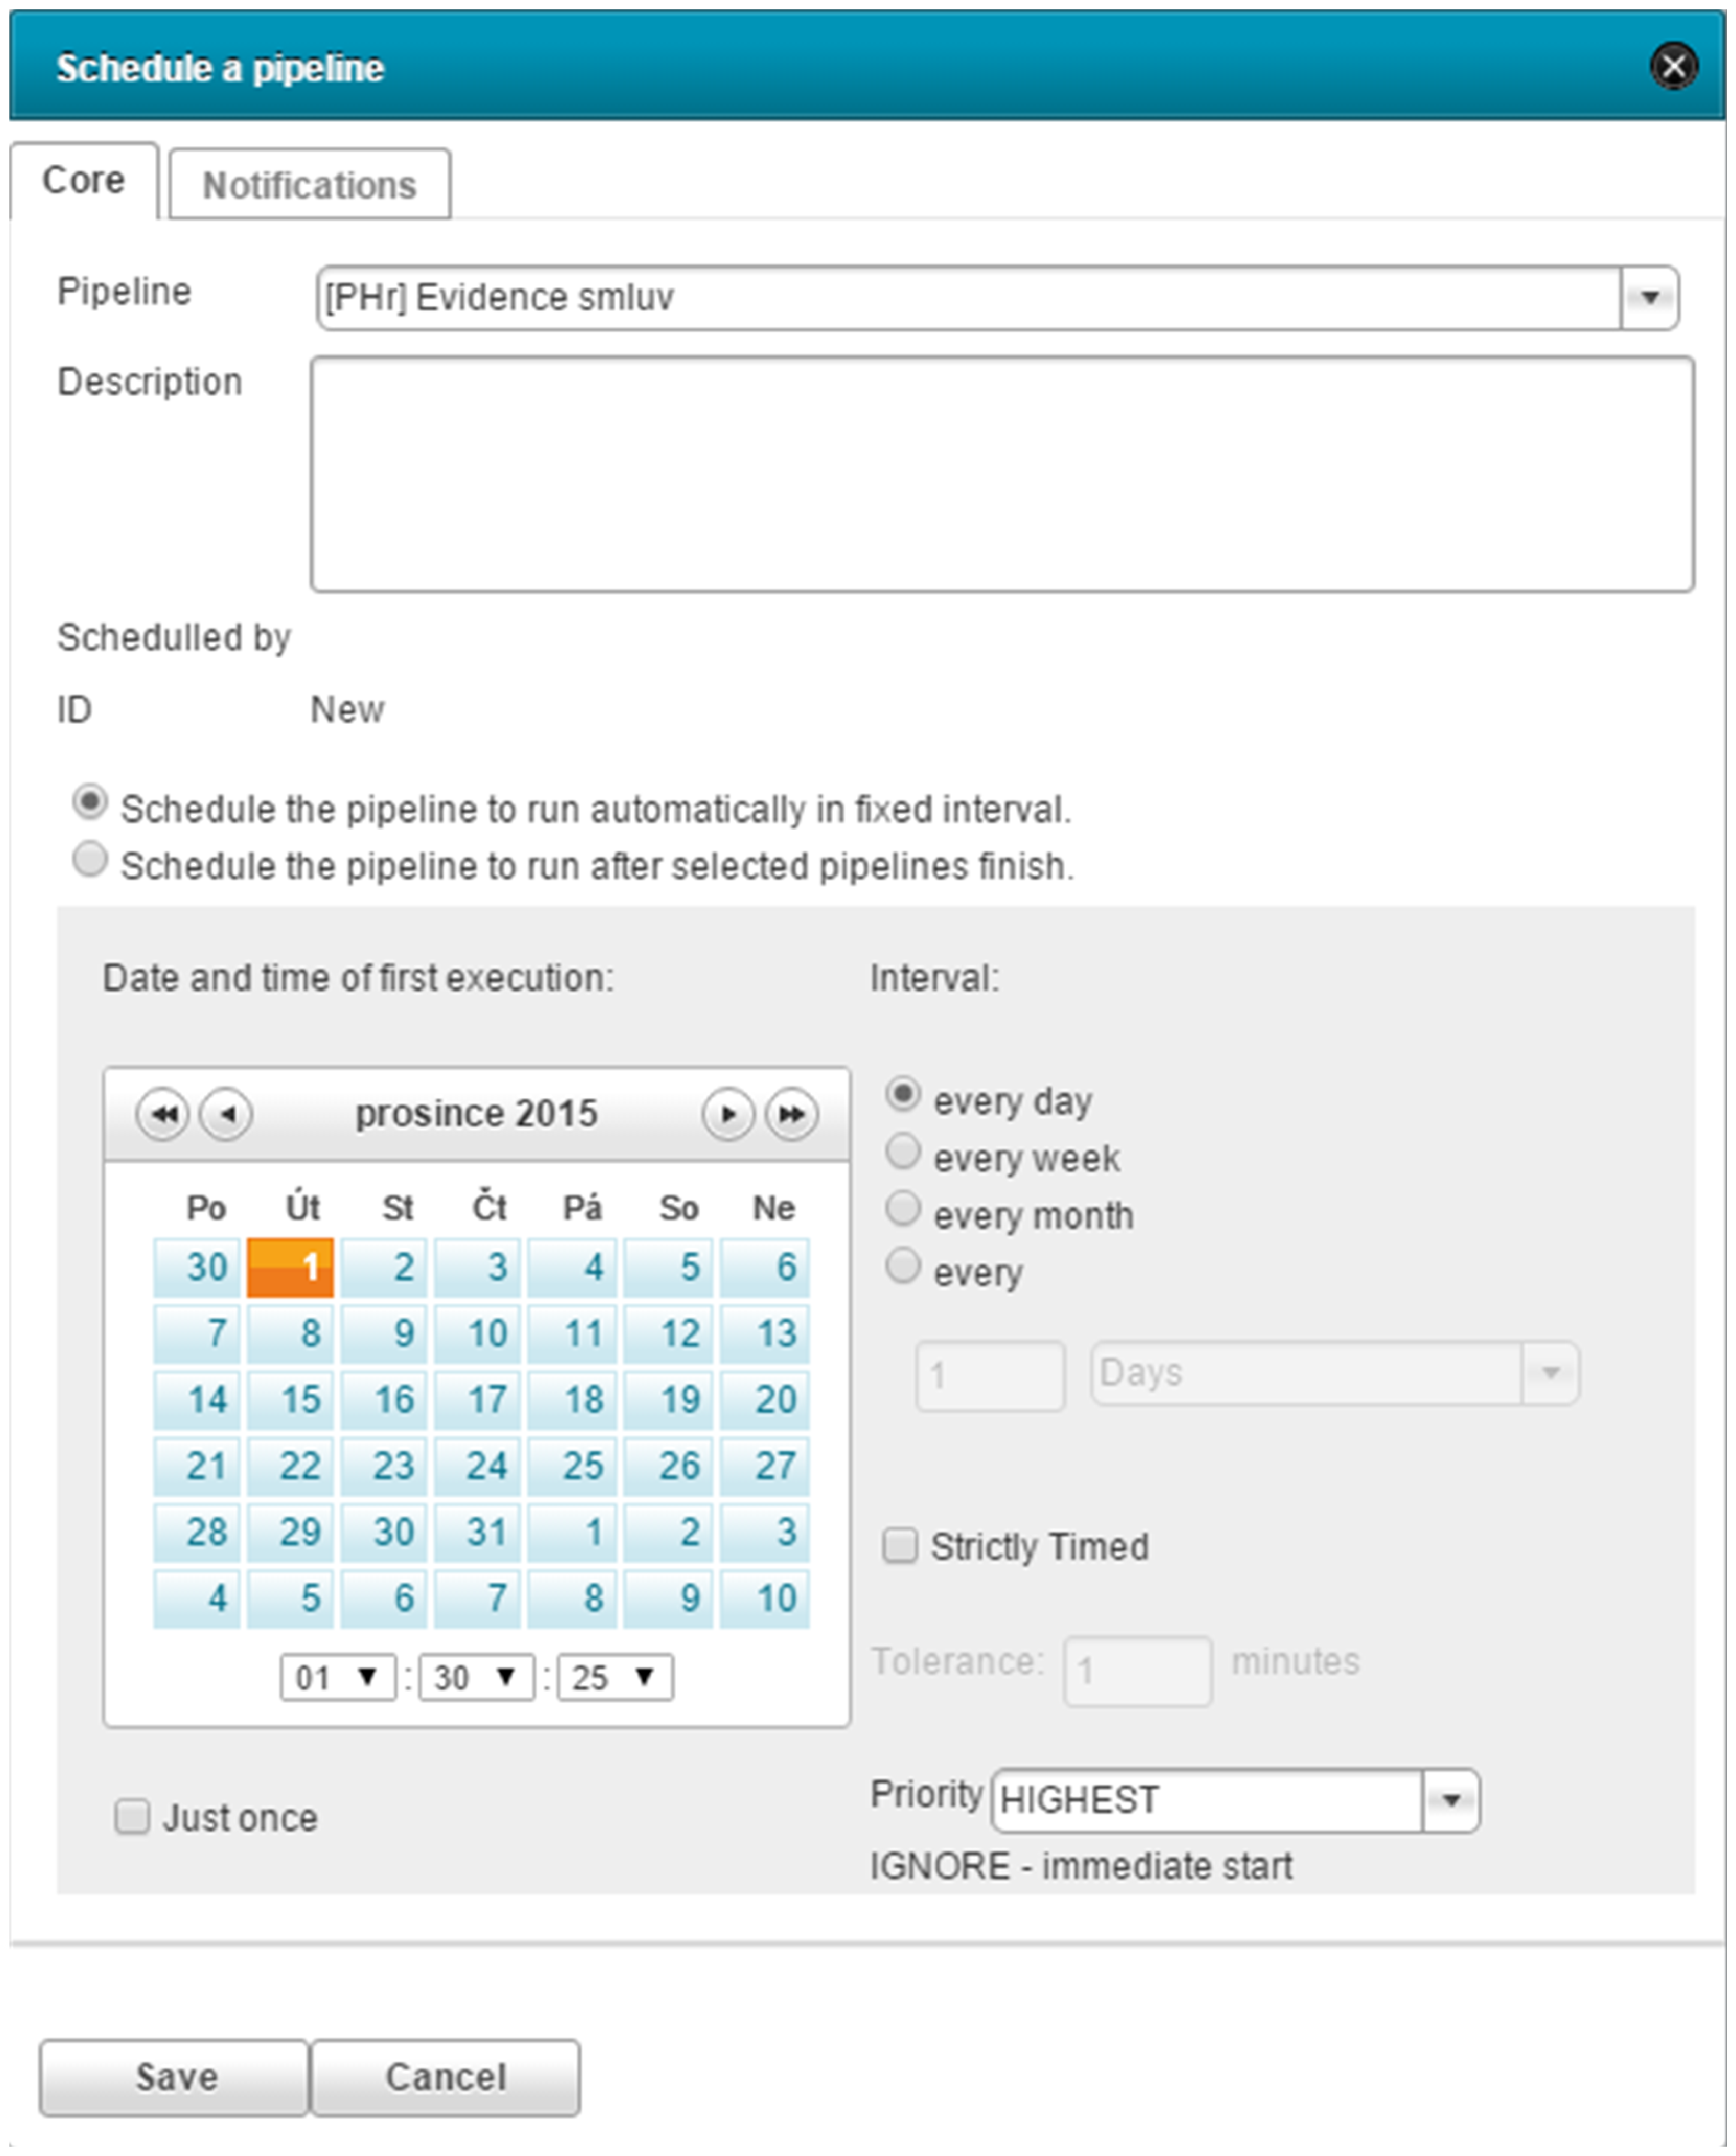
\includegraphics[width=80mm]{img/unvSchedule.eps}}
\caption{Nastavení intervalu exekuze pipeline nástroji UV}
\label{obr:unvSchedule}
\end{figure}

\section{Webová aplikace}

\subsection{Volba technologií a implementační platformy}

Webová aplikace je implementována také v technologii ASP.Net se zvoleným architektonickým vzorem MVC. K práci s RDF daty využijeme také knihovnu dotnetRdf. Layout aplikace je tvořen formou responzivního Bootstrap designu. Aplikace se skládá z pěti pohledů: Úvodní obrazovka, Detail subjektu, Detail smlouvy, Veřejné zakázky subjektu a O aplikaci.

\subsection{Získávání dat}

V rámci aplikace využíváme přístup k datovým sadám z těchto SPARQL endpointů:

\begin{itemize}
\item Otevřené smlouvy - http://student.opendata.cz/sparql
\item Organizace, ARES, Orgány veřejné moci - http://linked.opendata.cz/sparql
\item RÚIAN - http://ruian.linked.opendata.cz/sparql
\item DBpedia - http://dbpedia.org/sparql, nebo česká verze http://cs.dbpedia.org/sparql
\end{itemize}

Konkrétní data se získávají pomocí SPARQL dotazů popsaných níže v rámci popisu jednotlivých pohledů\footnote{Položky uvedené znakem "@" jsou proměnné}.

\subsubsection*{Úvodní obrazovka}

Úvodní obrazovku můžeme rozdělit do pomyslných tří částí. 

První částí je hlavička obsahující odkazy na web Iniciativy za otevřenou datovou infrastrukturu\cite{od}, datový standard pro otevřené smlouvy\cite{metodika} a informace o aplikaci.

Druhou částí je zobrazení vydavatelů na mapovém podkladu. Nejdříve získáme informace o subjektech pomocí SPARQL dotazu \ref{lst:getPublishers} (endpoint Otevřené smlouvy). Posléze pro každý subjekt nalezneme jeho link pro přístup k RÚIANU dotazem \ref{lst:getBusinessEntityRuianLink} (endpoint Organizace, ARES, Orgány veřejné moci). Pomocí obdrženého linku získáme informace o adresním místu z RÚIANu dotazem \ref{lst:getBusinessEntityCoordinates} (endpoint RÚIAN). Na závěr zkusíme získat foto subjektu z DBpedie dotazem \ref{lst:getPublisherImage} (endpoint DBpedia). Získané informace zobrazíme uživateli na mapovém podkladu. Každý subjekt je zvýrazněn na svých souřadnicích\footnote{Počet otevřených smluv je v mapě znázorněn červeným kruhem. Ti, co jich mají více, jsou výraznější.}. Po kliku na subjekt se otevře informační okno s podrobnostmi s možností přejití na detail subjektu.

Třetí částí je seznam smluv. Smlouvy získáme pomocí SPARQL dotazu \ref{lst:getContracts} (endpoint Otevřené smlouvy) (Viz Obr. \ref{obr:mainPage}).\\

\begin{figure}[H]
\centerline{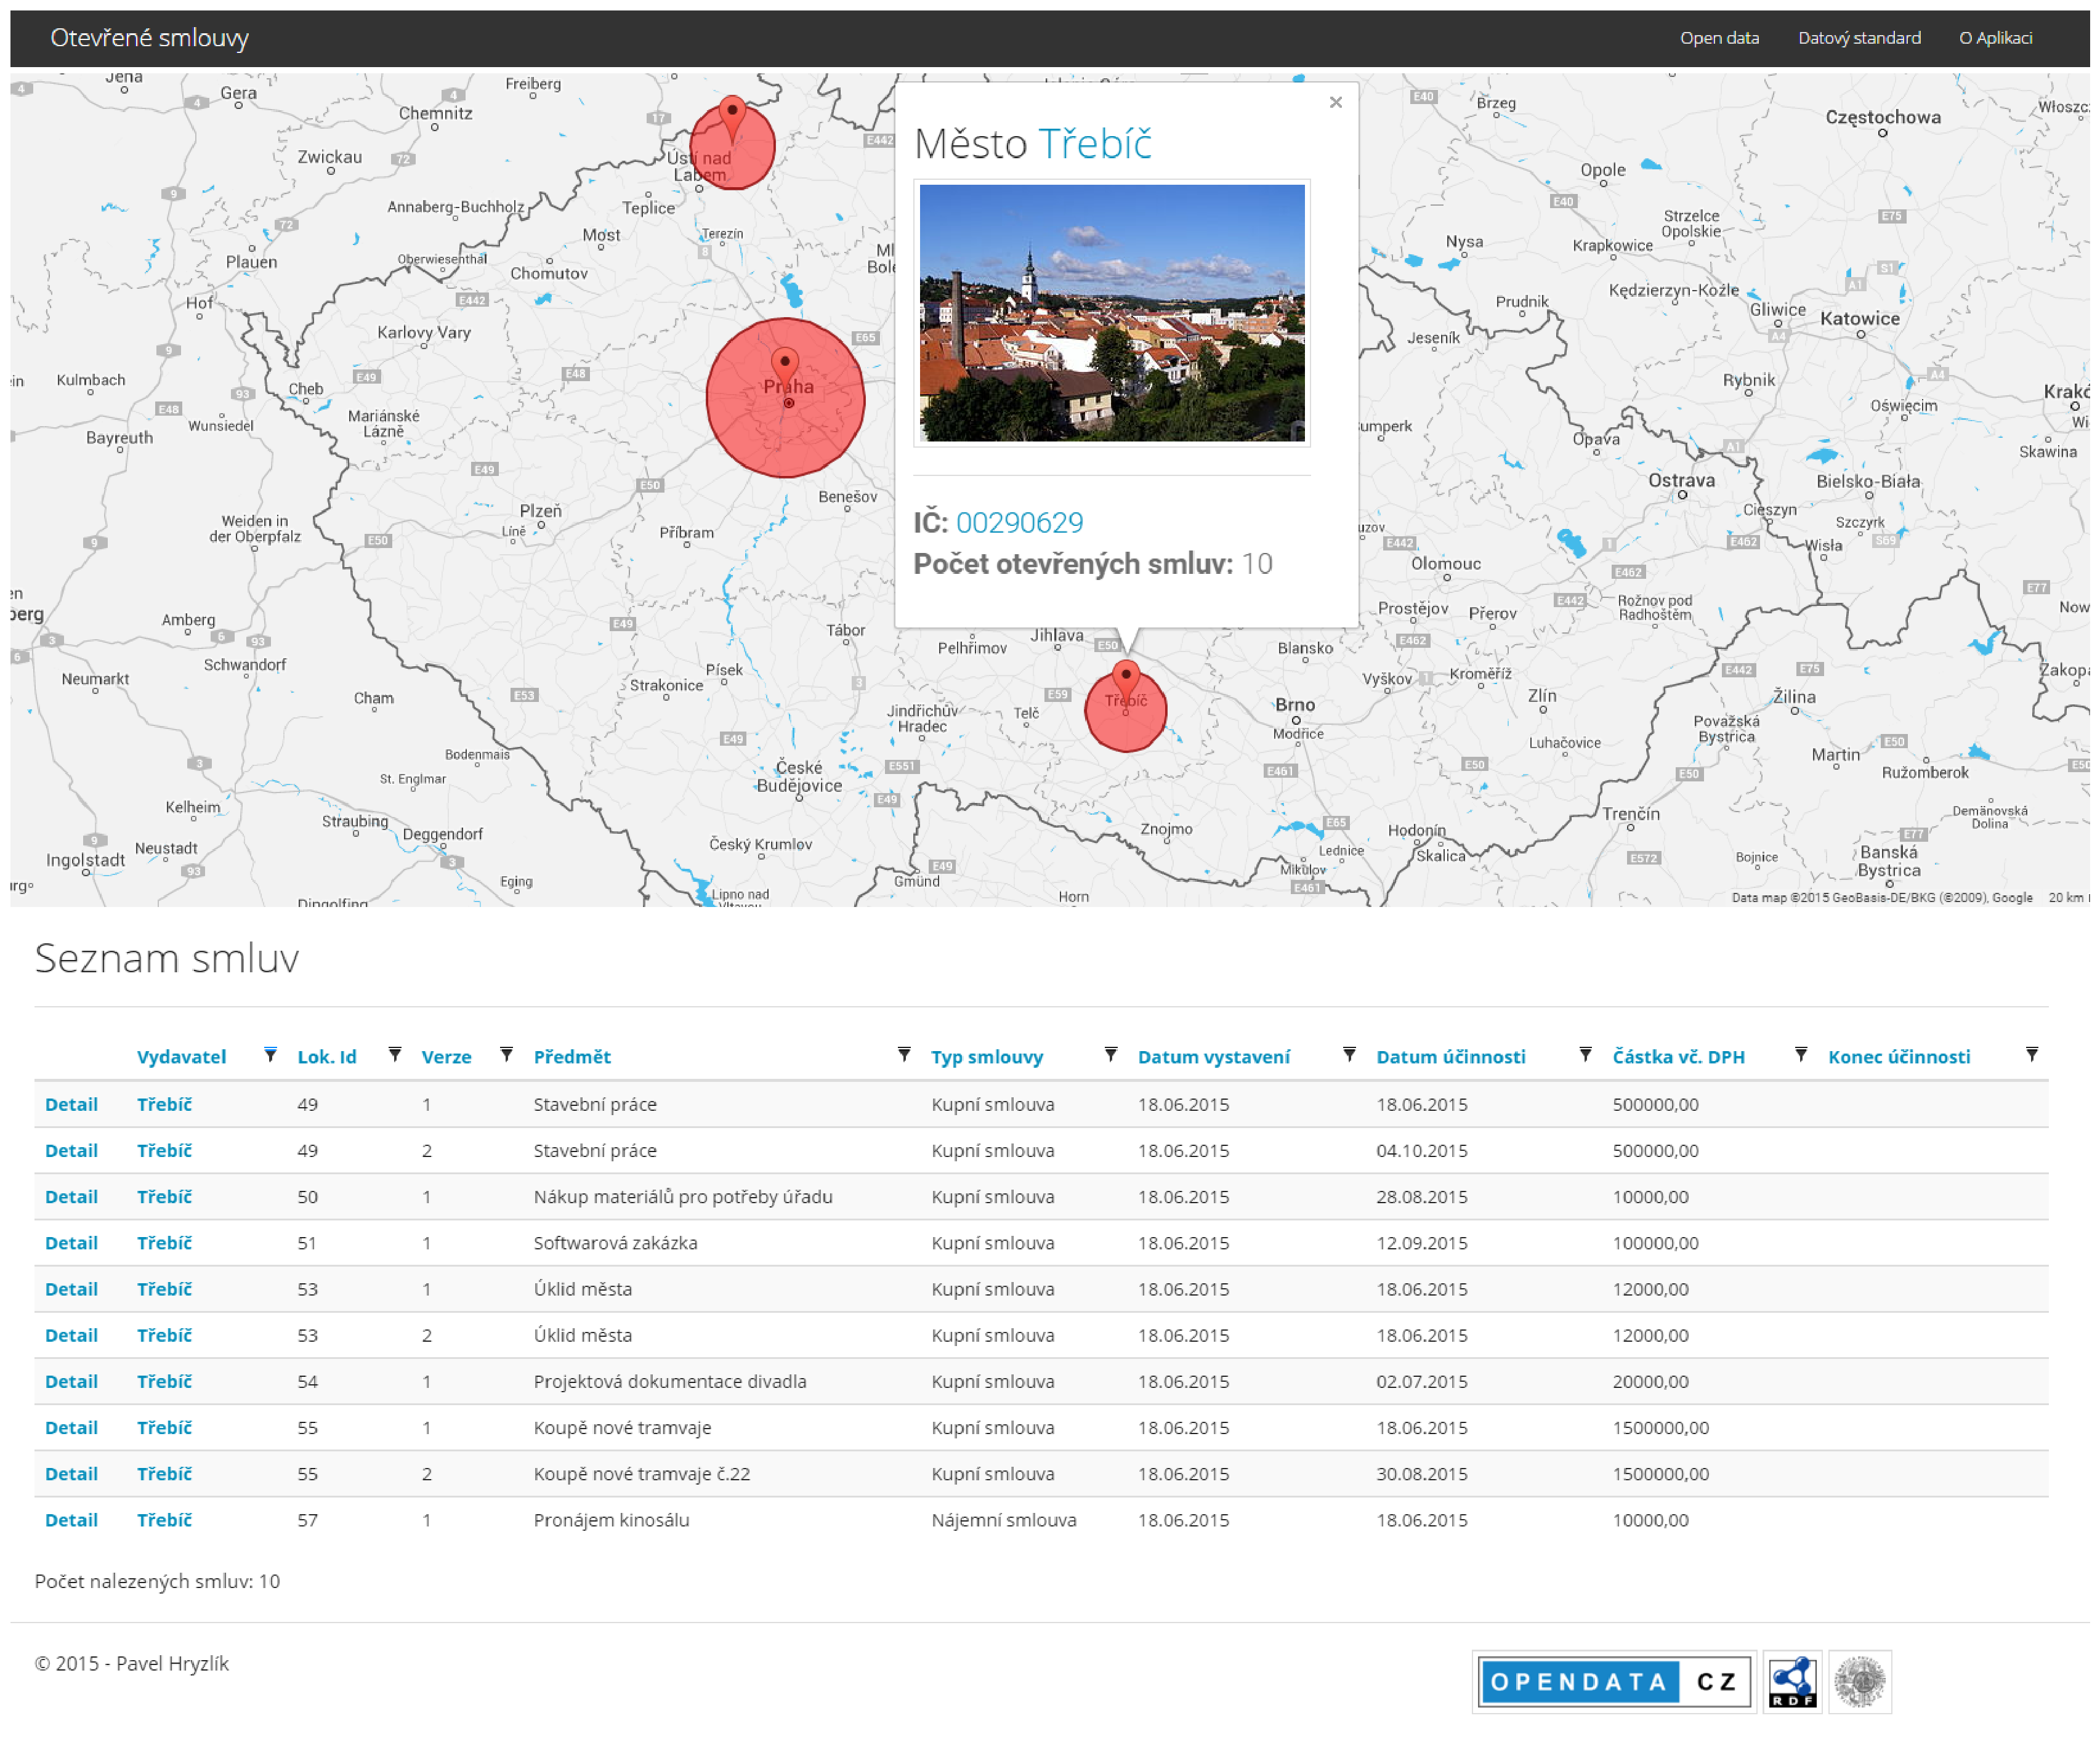
\includegraphics[width=\textwidth]{img/webMainPage.eps}}
\caption{Úvodní obrazovka webové aplikace}
\label{obr:mainPage}
\end{figure}

\lstinputlisting[label=lst:getPublishers, caption=Získej informace o subjektech, language=XML]{code/getPublishers.sparql}

\lstinputlisting[label=lst:getBusinessEntityRuianLink, caption=Získej adresní místo, language=XML]{code/getBusinessEntityRuianLink.sparql}

\lstinputlisting[label=lst:getBusinessEntityCoordinates, caption=Získej polohu subjektu, language=XML]{code/getBusinessEntityCoordinates.sparql}

\lstinputlisting[label=lst:getPublisherImage, caption=Získej foto subjektu, language=XML]{code/getPublisherImage.sparql}

\lstinputlisting[label=lst:getContracts, caption=Získej všechny smlouvy, language=XML]{code/getContracts.sparql}

\subsubsection*{Detail subjektu}

Detail subjektu nabízí podrobné informace o vydavateli a seznam jeho smluv. Informace o subjektu získáme na základě jeho IČ dotazem \ref{lst:getPublisherByIc} (endpoint Otevřené smlouvy). Další informace získáme podobně jako na úvodní obrazovce dotazy \ref{lst:getBusinessEntityRuianLink},\ref{lst:getPublisherImage}. Jako informaci navíc zkusíme zjistit informace o otevíracích dobách vydavatele dotazem \ref{lst:getBusinessEntityOpeningHours} (endpoint Organizace, ARES, Orgány veřejné moci). Posléze nad endpointem Otevřené smlouvy obdržíme seznam smluv subjektu pomocí dotazu \ref{lst:getContractByPublisheIc} (Viz Obr. \ref{obr:webSubjectDetail}).\\

\begin{figure}[H]
\centerline{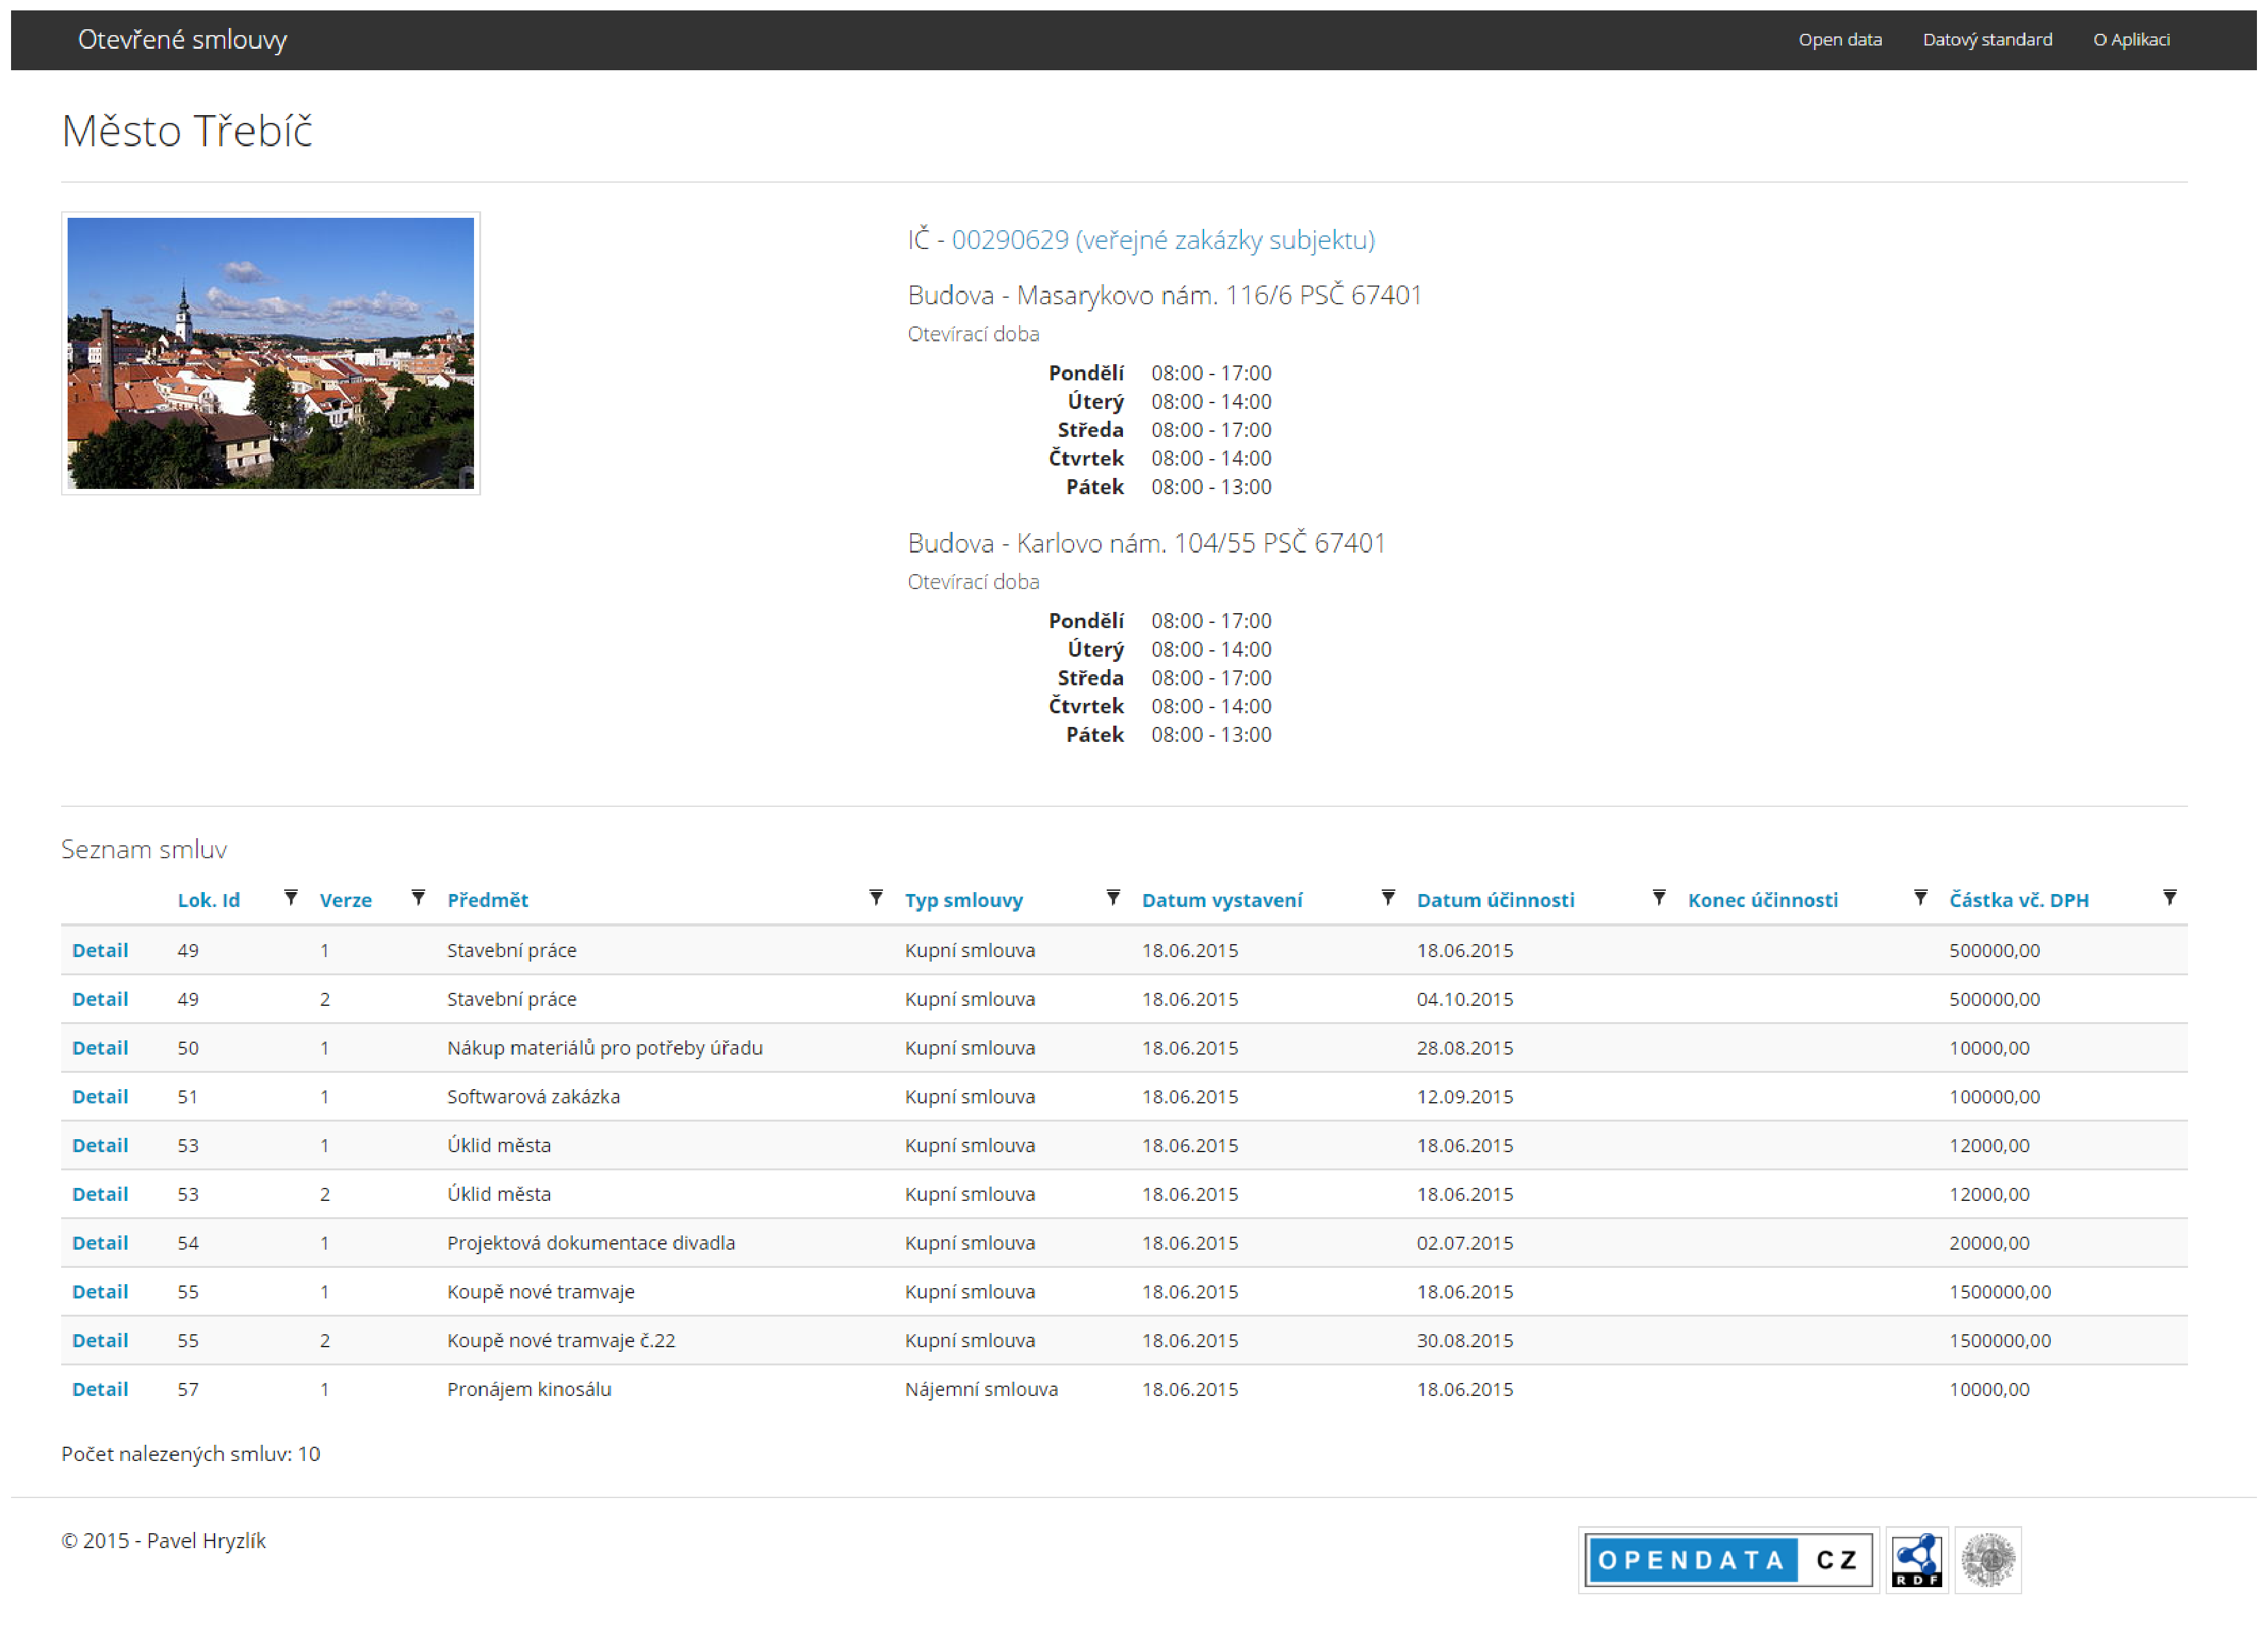
\includegraphics[width=\textwidth]{img/webSubjectDetail.eps}}
\caption{Obrazovka detailu subjektu}
\label{obr:webSubjectDetail}
\end{figure}

\lstinputlisting[label=lst:getPublisherByIc, caption=Získej vydavatele na základě IČ, language=XML]{code/getPublisherByIc.sparql}

\lstinputlisting[label=lst:getBusinessEntityOpeningHours, caption=Získej otevírací hodiny subjektu, language=XML]{code/getBusinessEntityOpeningHours.sparql}

\lstinputlisting[label=lst:getContractByPublisheIc, caption=Získej všechny smlouvy daného vydavatele, language=XML]{code/getContractByPublisheIc.sparql}


\subsubsection*{Detail smlouvy}

Jak název napovídá, detail smlouvy poskytuje podrobné informace o smlouvě, smluvních stranách, přílohách, dodatcích, milnících, informacích o ceně a verzích smlouvy. Údaje získáme pomocí dotazů \ref{lst:getContract},\ref{lst:getPartiesByContract},\ref{lst:getAttachmentsByContract},\ref{lst:getAmendmentsByContract},\ref{lst:getMilestonesByContract},\ref{lst:getPriceSpecByContract},\ref{lst:getVersionsByContract} nad endpointem Otevřené smlouvy (Viz Obr. \ref{obr:contractDetail}).\\

\begin{figure}[H]
\centerline{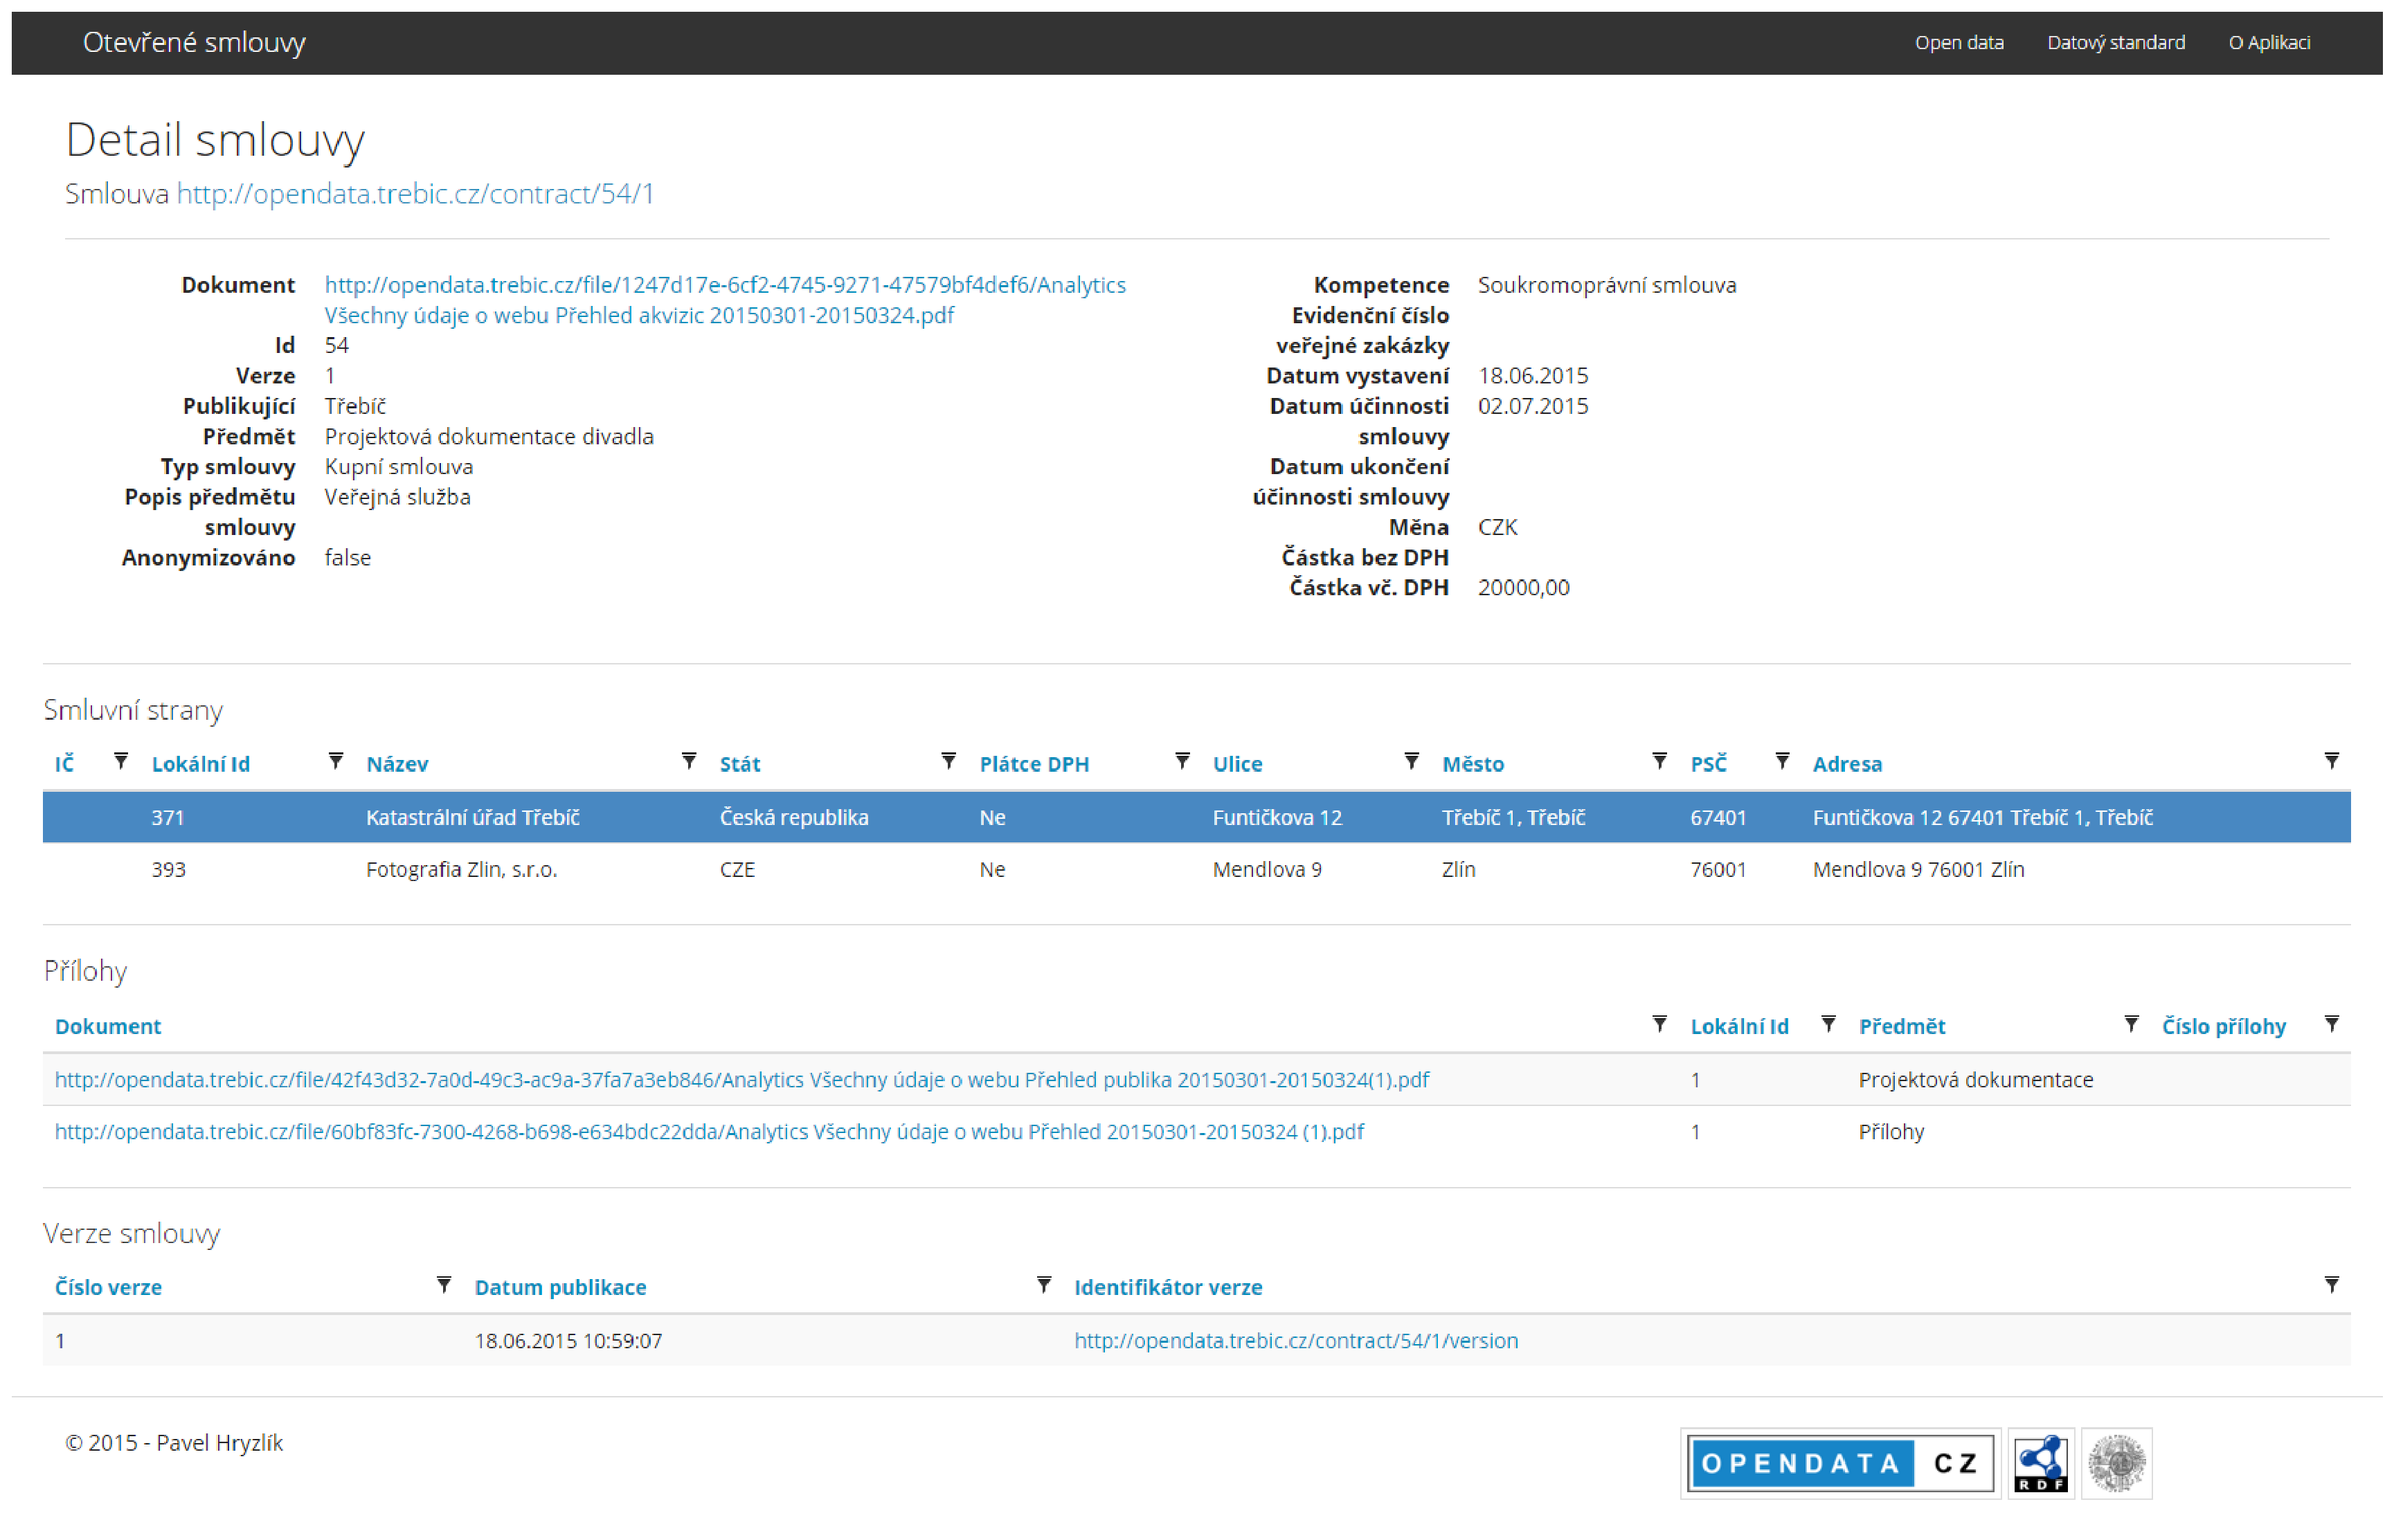
\includegraphics[width=\textwidth]{img/webContractDetail.eps}}
\caption{Obrazovka detailu smlouvy}
\label{obr:contractDetail}
\end{figure}

\lstinputlisting[label=lst:getContract, caption=Získej smlouvu, language=XML]{code/getContract.sparql}

\lstinputlisting[label=lst:getPartiesByContract, caption=Získej smluvní strany na základě smlouvy, language=XML]{code/getPartiesByContract.sparql}

\lstinputlisting[label=lst:getAttachmentsByContract, caption=Získej přílohy na základě smlouvy, language=XML]{code/getAttachmentsByContract.sparql}

\lstinputlisting[label=lst:getAmendmentsByContract, caption=Získej dodatky na základě smlouvy, language=XML]{code/getAmendmentsByContract.sparql}

\lstinputlisting[label=lst:getMilestonesByContract, caption=Získej milníky na základě smlouvy, language=XML]{code/getMilestonesByContract.sparql}

\lstinputlisting[label=lst:getPriceSpecByContract, caption=Získej informace o ceně, language=XML]{code/getPriceSpecByContract.sparql}

\lstinputlisting[label=lst:getVersionsByContract, caption=Získej verze smlouvy, language=XML]{code/getVersionsByContract.sparql}


\subsubsection*{Veřejné zakázky subjektu}

Seznam veřejných zakázek je dostupný z detailu subjektu na základě jeho IČ. Získáme jej dotazem \ref{lst:getBusinessEntityPublicContracts} (endpoint Organizace, ARES, Orgány veřejné moci) (Viz Obr. \ref{obr:webPublicContracts}).\\

\begin{figure}[H]
\centerline{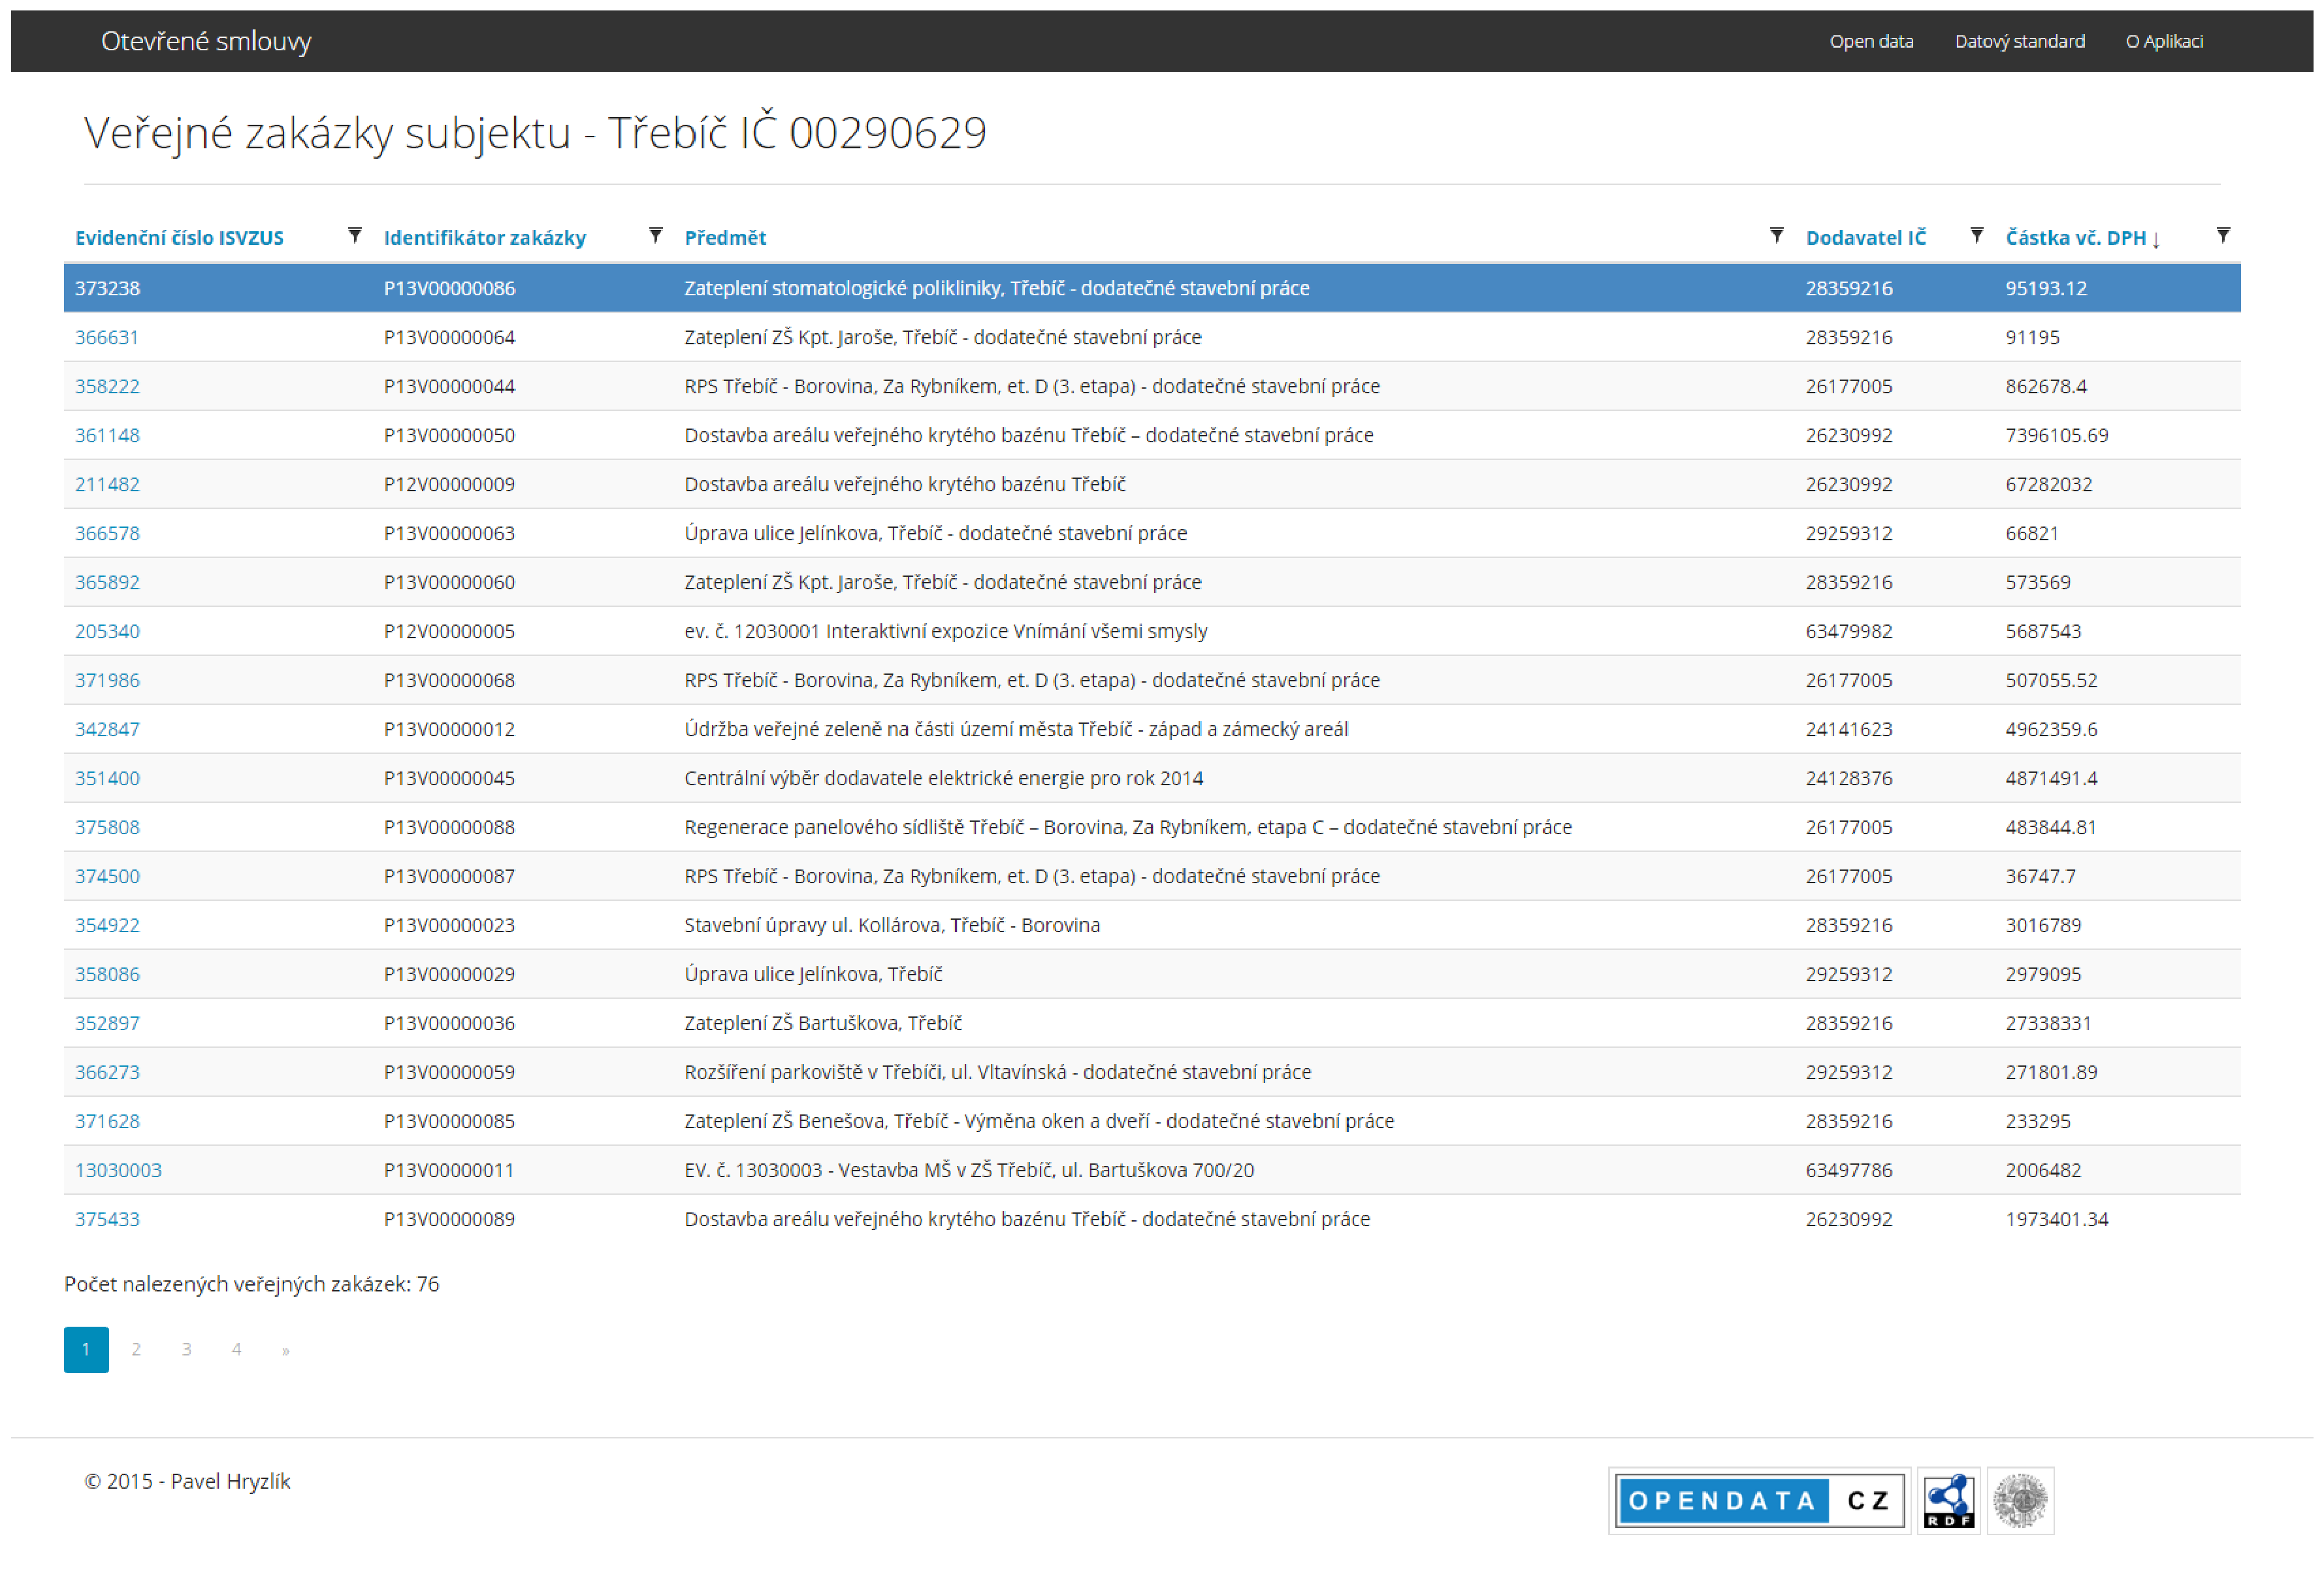
\includegraphics[width=\textwidth]{img/webPublicContracts.eps}}
\caption{Obrazovka seznamu veřejných zakázek subjektu}
\label{obr:webPublicContracts}
\end{figure}

\lstinputlisting[label=lst:getBusinessEntityPublicContracts, caption=Získej veřejné zakázky na základě subjektu, language=XML]{code/getBusinessEntityPublicContracts.sparql}

\subsubsection*{O aplikaci}

V rámci tohoto pohledu jsou uvedeny základní informace o projektu.

\subsection{Požadavky na architekturu}

Pro implementaci jsme zvolili technologii ASP.Net s architektonickým vzorem MVC. Procesním a endpoint modulem je tedy v tomto případě Controller, který na základě klientských požadavků volá odpovídající SPARQL dotazy získávající data z různých zdrojů (endpointů). Komunikace mezi procesním a prezentačním modelem (Komunikační modul) je řešena interně v rámci technologie ASP.Net. V rámci architektury MVC je prezentačním modulem část View obsahující jednotlivé pohledy popsané výše.



\chapter{Evaluace}

V rámci této kapitoly se zaměříme na otestovaní konverzního mechanismu platformy nad daty nastiňující reálnou situaci na úřadech.

V únoru roku 2015 vydalo Ministerstvo vnitra dopadovou studii na odhad nákladů k zavedení zákona o registru smluv\footnote{http://www.janfarsky.cz/wp-content/uploads/2015/05/Dopadov\%C3\%A1-studie-ke-KPN-k-registru-smluv-PRACOVNI-VERZE-27-02-2015-1.pdf}. V reakci na tento odhad nedlouho poté vydalo Cetrum aplikované ekonomie o.s. stínový výpočet korigující výsledky Ministerstva vnitra\footnote{ http://www.rekonstrukcestatu.cz/publikace/2015-03-04-stinovy-vypocet-ria-k-registru-smluv.pdf}. Na základě těchto studií můžeme získat hrubou představu o tom, kolik jednotlivé subjekty cca uzavírají nedlouho poté smluv. Veřejné instituce tak rozdělíme do čtyř kategorií:  

\begin{itemize}
\item Malé - Nejmenší instituce, uzavírající jednotky smluv měsíčně s celkovým úhrnem maximálně několika desítek smluv ročně (v rámci měst a obcí jde o nejvyšší zastoupení).
\item Střední - Subjekty generující maximálně desítky smluv měsíčně, s jednotkami stovek smluv ročně (v rámci všech subjektů pravděpodobně nevýznamnější zastoupení). 
\item Středně velké - Instituce, které produkují desítky, až stovky smluv měsíčně s jednotkami tisíců smluv ročně.
\item Velké - Velké instituce se stovkami až tisíci smluv měsíčně s roční produkcí tisíců až desetitisíců smluv.
\end{itemize}

Pro simulaci prostředí jednotlivých kategorií vytvoříme pro každou skupinu testovací relační databázi s desítkami, stovkami, tisíci a desetitisíci smluv. Nad každou databází spustíme konverzní modul a změříme dva pravděpodobně nejčastější požadavky - dump dat, resp. výčet všech smluv a vyhledání jedné konkrétní smlouvy. Dump je základní funkcionalitou k vypublikování otevřených smluv. Potřebujeme ho také v rámci platformy, resp. jednotného úložiště, které dílčí dumpy stahuje. Ukázka vyhledání jedné smlouvy slouží spíše k ukázce, že konverzní modul půjde využít i mimo platformu, např. v rámci webových stránek konkrétní veřejné instituce.   

Pro generování dat v SQL databázi byl zvolen nástroj Sql Data Generator\footnote{TODO - odkaz na zdroj.}. Tento nástroj umožňuje nastavení nejen počtu vygenerovaných dat, ale i např. procentuální zastoupení propojení tabulek nebo šablony pro konkrétní hodnoty v jednotlivých sloupcích. Umožní nám přiblížit se k reálnému obsahu databází veřejných institucí\footnote{Pro představu je příklad XML scriptu přiložen na datovém nosiči. Sql Data Generator je ale komerční nástroj, který neumožňuje zobrazit generovaný sql příkaz.}. K samotnému profilingu využijeme klasických prostředků prostředí .Net. Změříme dobu od přijmutí požadavku po jeho kompletní zpracování.
\newpage

Měření probíhalo na sestavě:
\begin{itemize}
\item Intel Core i5-4200U, CPU @ 1.60GHz - 2.30GHz
\item 4GB RAM
\item 64bit operační systém
\item Databáze - MS SQL 2014
\end{itemize}

Pro každou kategorii bylo provedeno 15 měření pro dump, resp. vyhledání smlouvy. Z každé sady výsledků se odebrala minimální a maximální hodnota a následně ze zbývajících hodnot byl vypočítán průměr. Pro názornost, u dumpu uvádíme také velikost výstupních dat a počet vygenerovaných trojic. Výsledky lze najít v následujících grafech (\ref{obr:graphDump1},\ref{obr:graphDump2},\ref{obr:graphGet1}).

\begin{figure}[H]
\centerline{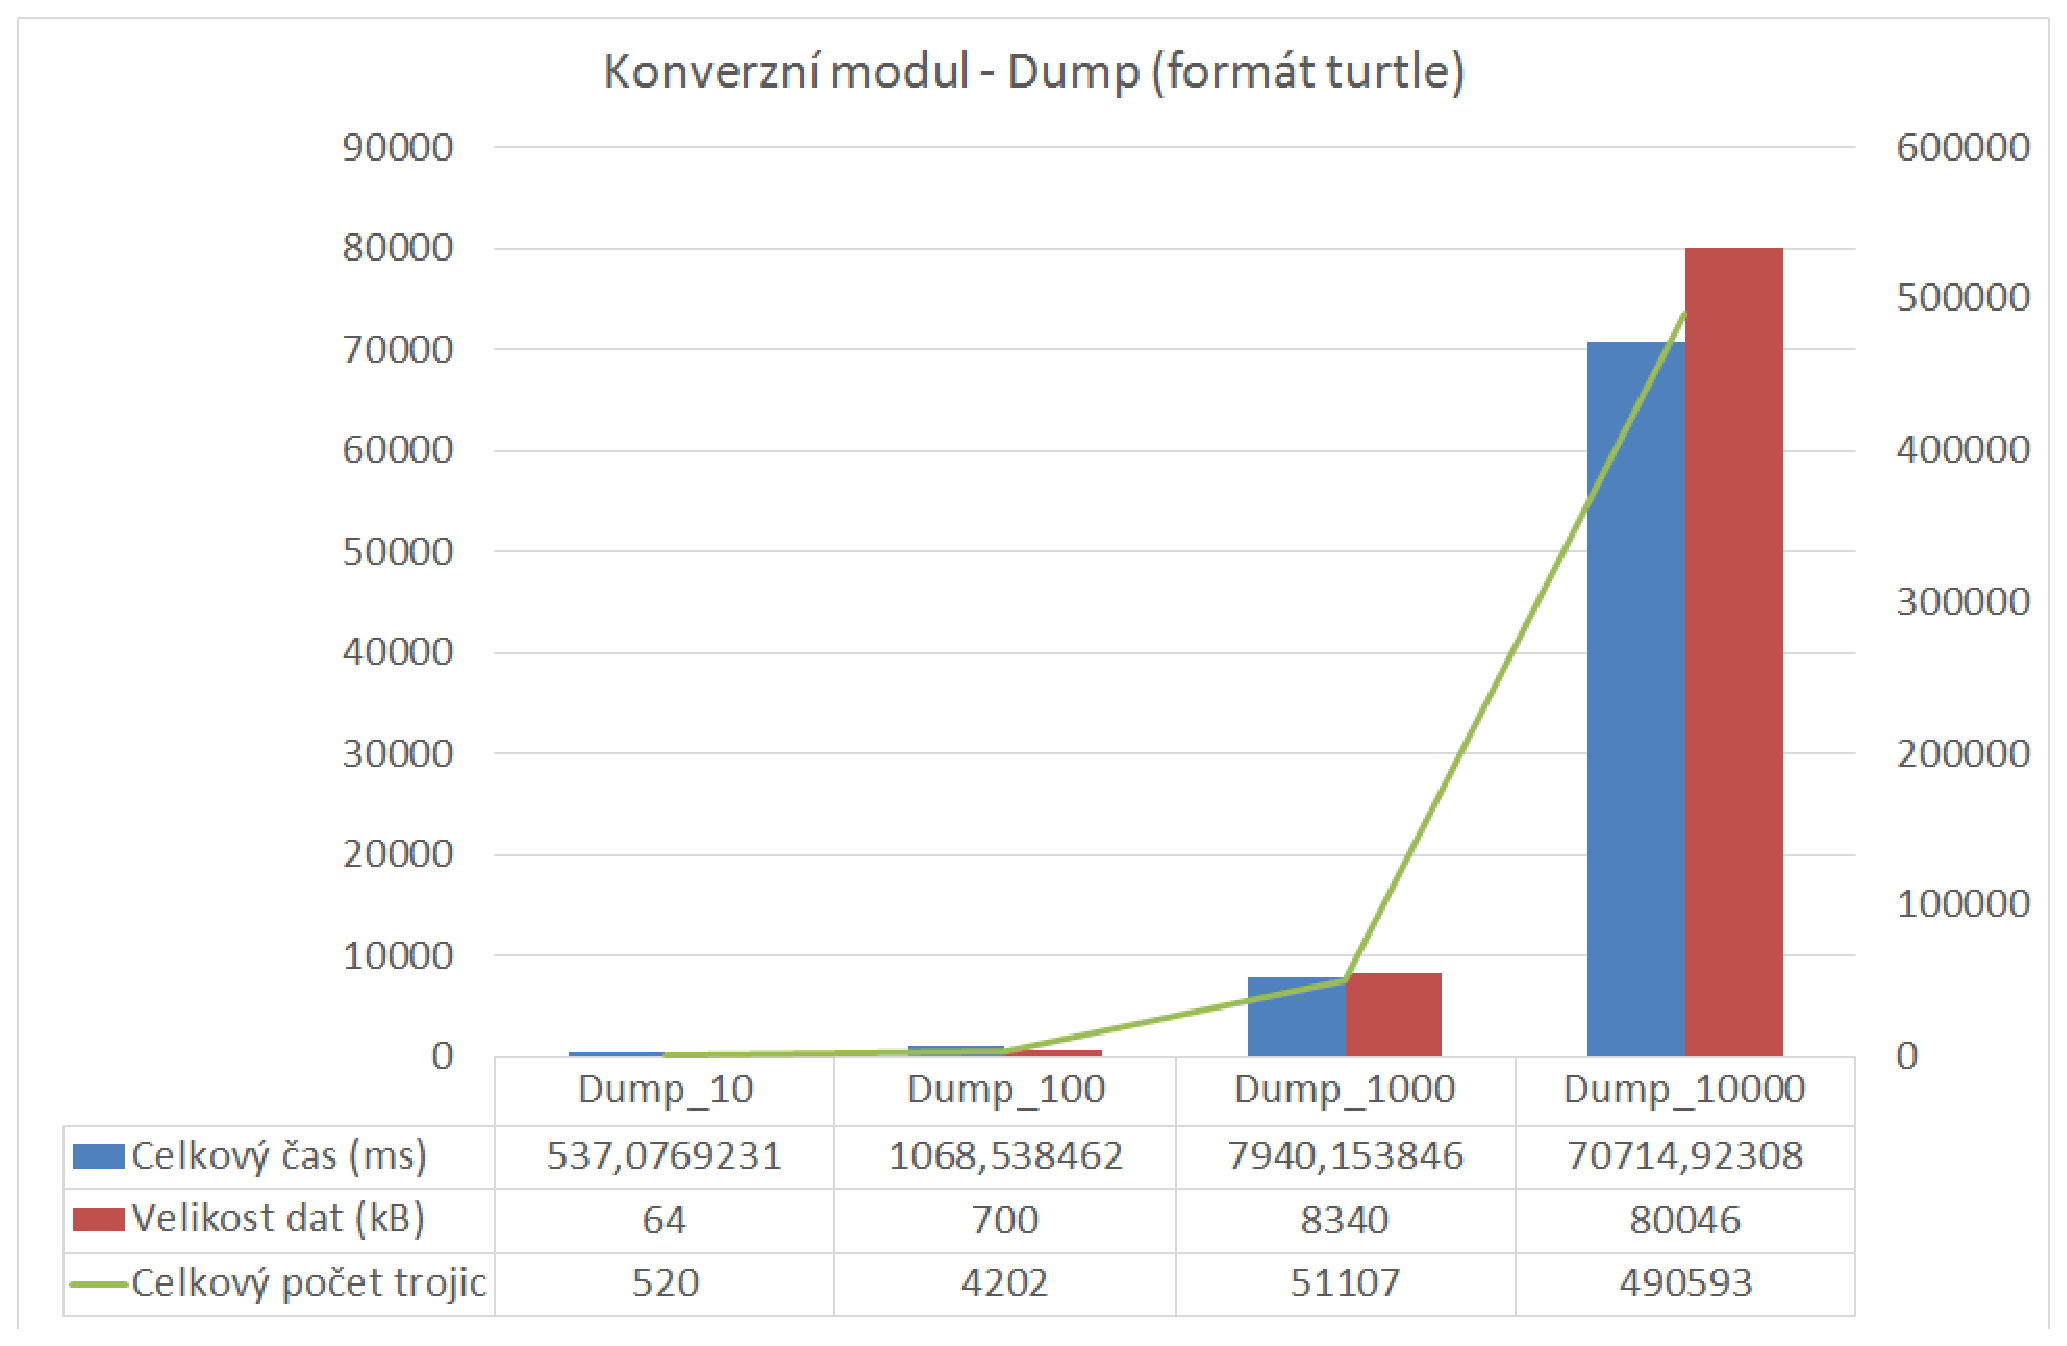
\includegraphics[width=\textwidth]{img/graphDump1.eps}}
\caption{Znázornění časové náročnosti dumpu vybraných dat}
\label{obr:graphDump1}
\end{figure}

\begin{figure}[H]
\centerline{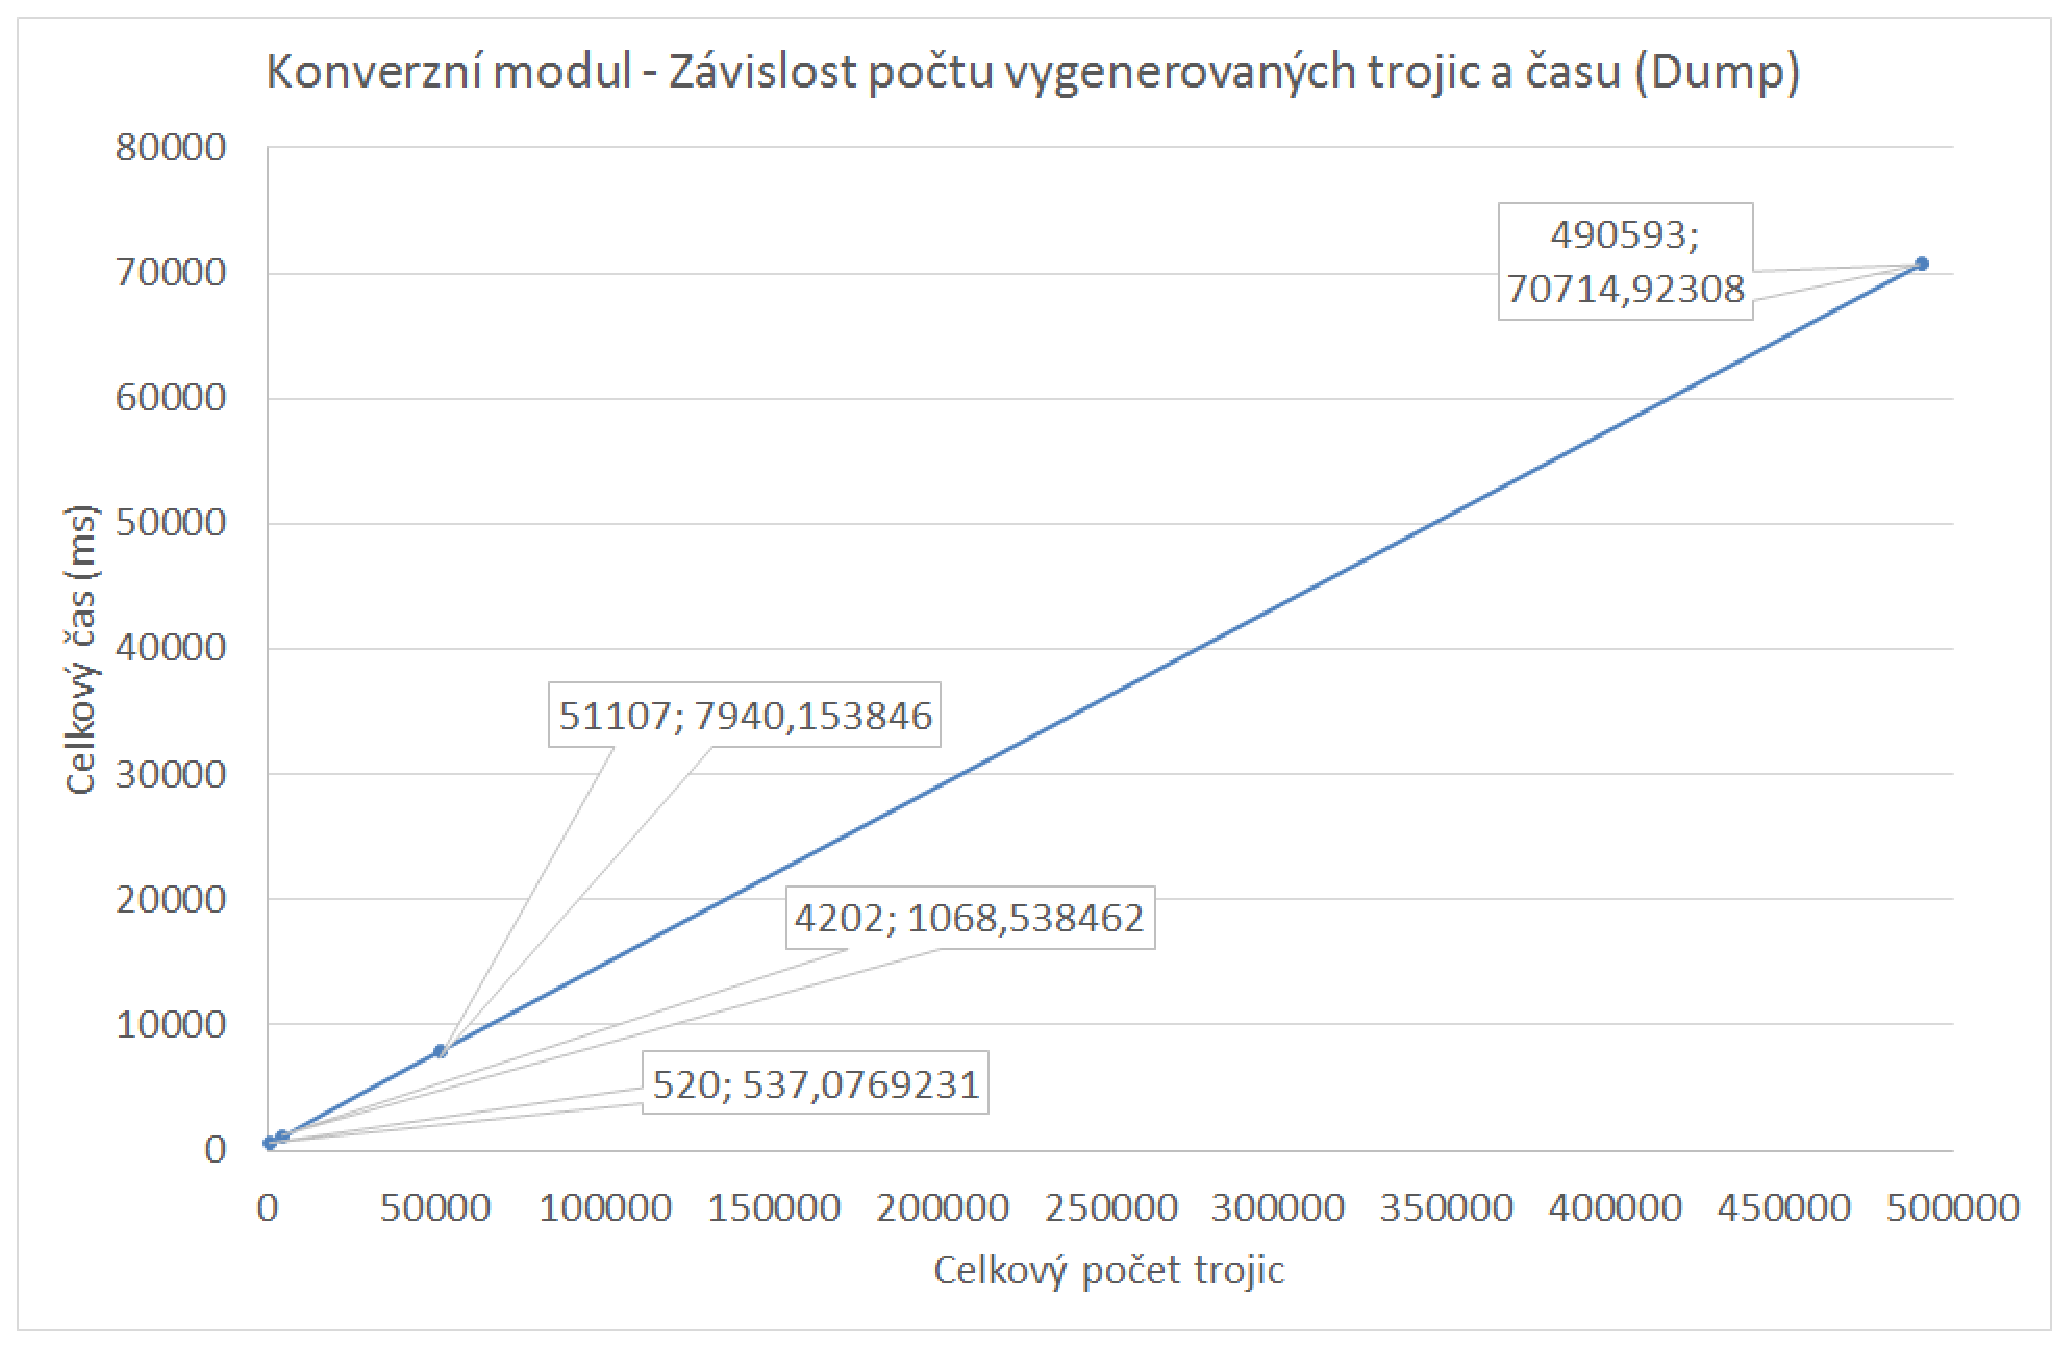
\includegraphics[width=\textwidth]{img/graphDump2.eps}}
\caption{Znázornění vztahu počtu vygenerovaných trojic a času při dumpu vybraných dat}
\label{obr:graphDump2}
\end{figure}

\begin{figure}[H]
\centerline{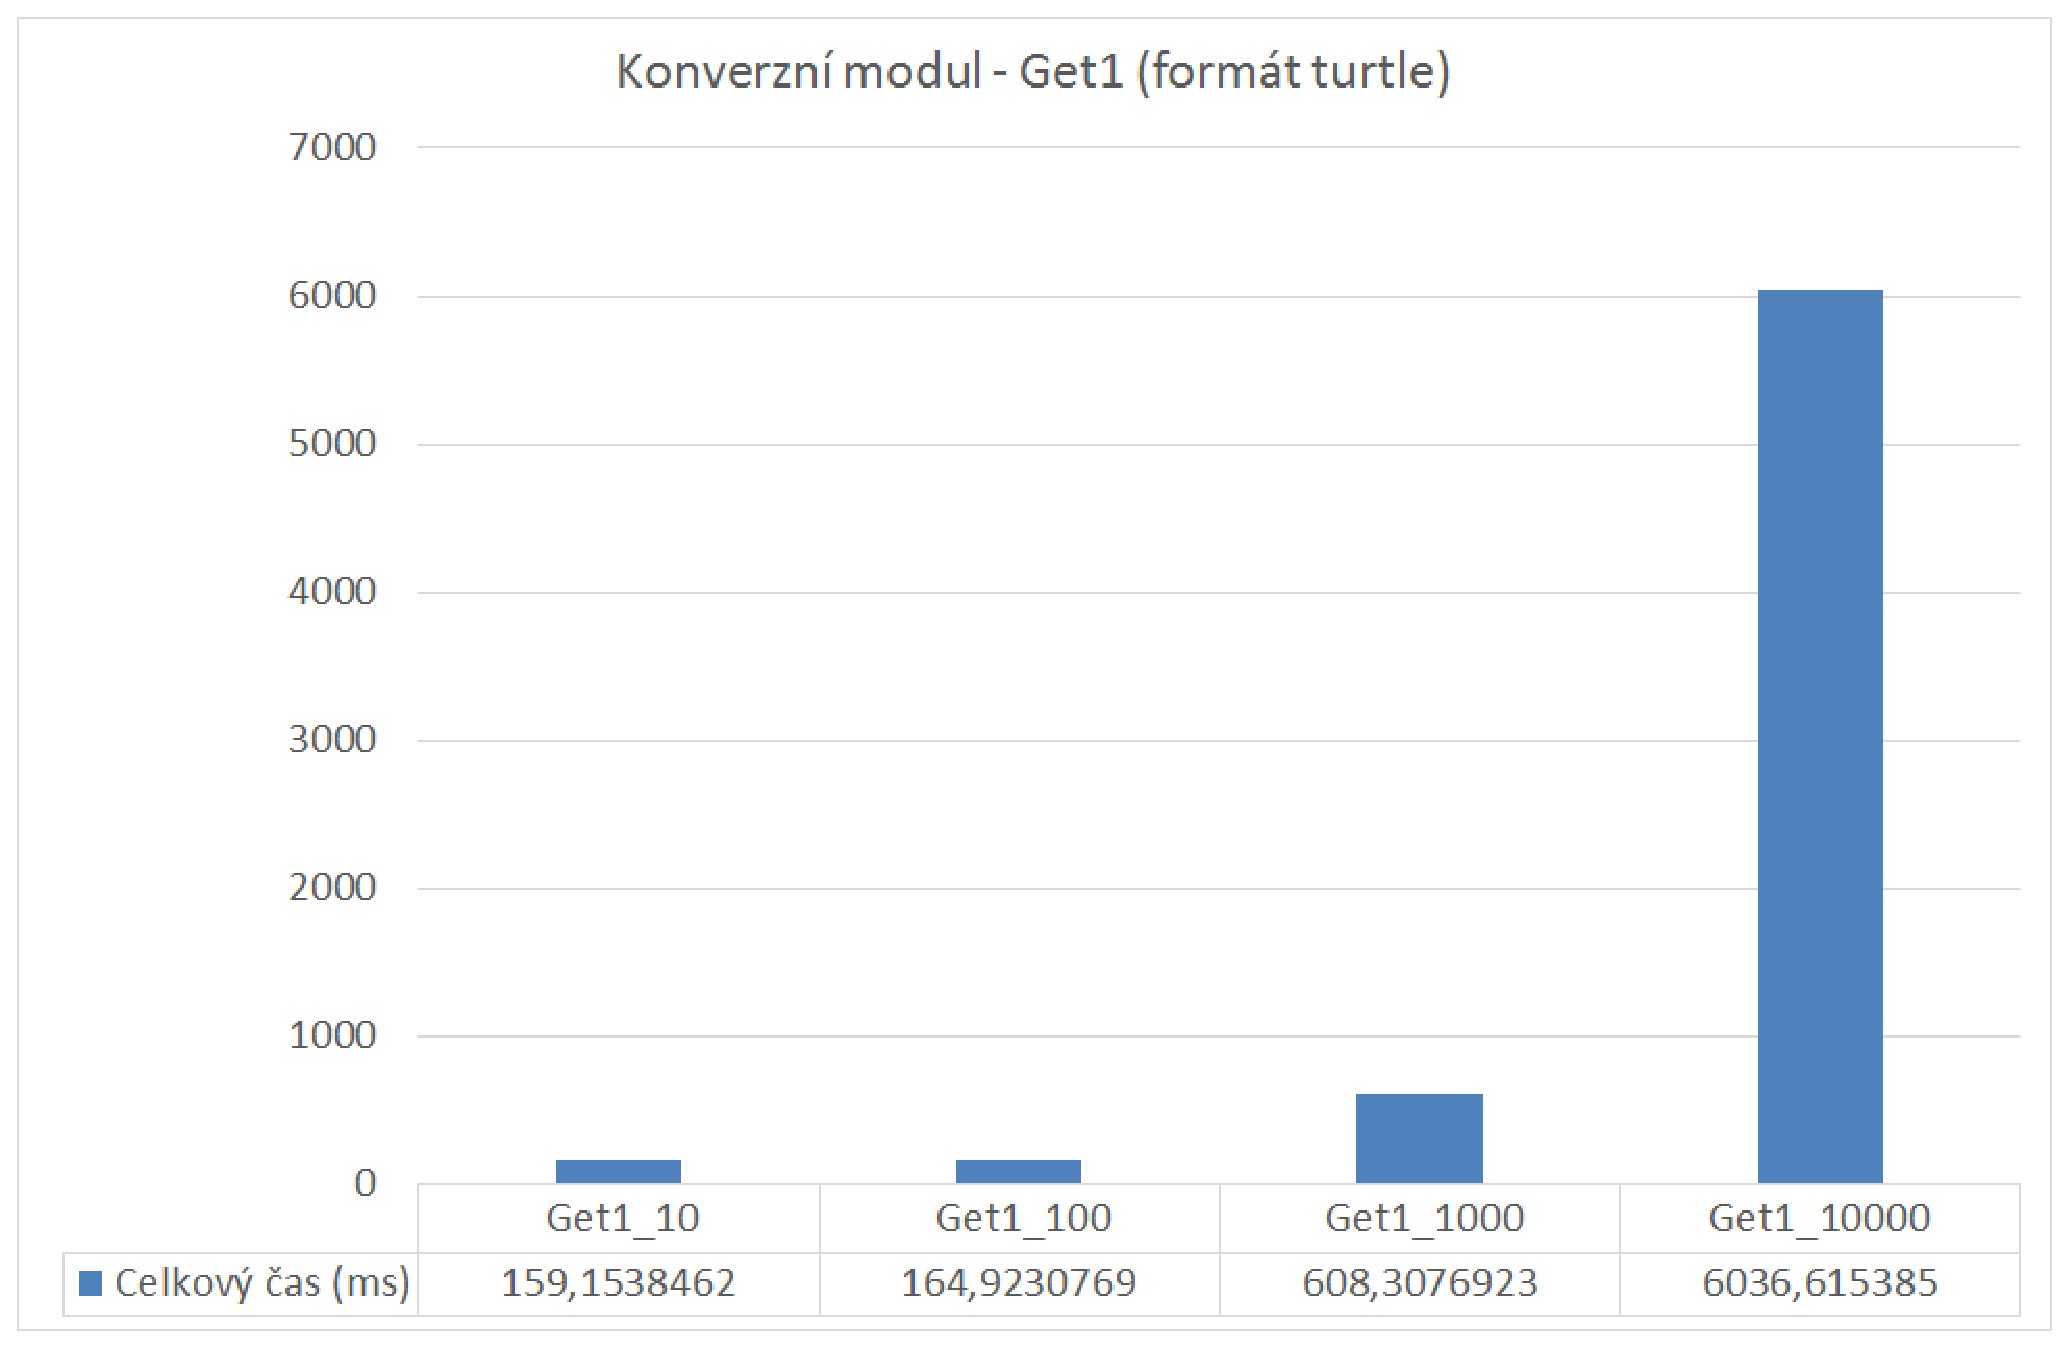
\includegraphics[width=\textwidth]{img/graphGet1.eps}}
\caption{Znázornění časové náročnosti získání jedné smlouvy u vybraných dat}
\label{obr:graphGet1}
\end{figure}

\newpage
Z výsledků lze konstatovat, že výkon klesá cca lineárně s množstvím dat (viz. graf \ref{obr:graphDump2}). Můžeme říci, že konverzní modul je schopen poskytovat základní funkcionalitu v rozumném čase u menších, středních i středně velkých institucí. U velkých institucí už výsledky nejsou ideální. Institucí publikujících takové množství smluv je ale v prostředí České republiky velmi málo. Příslibem je také to, že využívaný R2RML procesor podléhá soustavnému vývoji a do budoucna lze očekávat výrazné zrychlení.

\chapter{Shrnutí procesu otevírání smluv}

Za účelem větší názornosti shrneme dosavadní proces otevírání smluv jedním diagramem (viz Obr. \ref{obr:openingContracts}). Diagram je rozdělen do tří řádků a tří sloupců. První řádek zachycuje proces otevírání dat. Druhý řádek znázorňuje otevírání dat s využitím prinicpů Linked Data. Třetím řádkem je zapojení relačních dat do procesu. V prvním sloupci se nacházíme na úrovni schématu. Zde definujeme standardy, ontologie, schémata. Druhý sloupec znázorňuje produkci otevřených a propojitelných dat. V třetím sloupci jsme na úrovni publikace dat, resp. serializace otevřených a propojitelných dat do přenositelných formátů.

Začátek procesu je v tvorbě schématu. V našem případě se jedná o datový standard pro otevřené smlouvy. Na základě schématu je v diagramu znázorněna možnost produkovat otevřená data. Ta jsou pak serializovatelná do konkrétních datových formátů. Lepšími datovými formáty jsou ale ty, které jsou definované pomocí schématu datového, pro naše účely se jedná o formát JSON. Z diagramu je vidět, že ze schématu vytvoříme datové JSON schéma, které je poté využitelné při publikaci dat.

Na základě schématu můžeme také nadefinovat RDF ontologii, díky které se dostaneme do světa Linked Data. V diagramu je obdobně jako u otevřených dat znázorněna možnost na základě ontologií produkovat Linked Data a ta pak serializovat do RDF datových formátů.

Speciálním případem serializace RDF dat jsou data ve formátu JSON-LD. Na základě schématu, resp. datového JSON schématu a RDF ontologie, můžeme vytvořit takový JSON-LD kontext, že výsledná vypublikovaná JSON-LD data budou naplňovat jak datový standard, tak i RDF ontologii.

Posledním krokem je zapojení relačních dat do procesu otevírání smluv. Tato relační data na základě relačního schématu, resp. jeho datového modelu a RDF ontologie, zkonvertujeme do Linked Data.

Lze si všimnout, že se nebavíme pouze o údajích o smlouvách. Tento postup lze obecně použít nejen pro smlouvy, ale i pro libovolnou jinou doménu.

\begin{figure}[H]
\centerline{\includegraphics[angle=90,width=\textwidth]{img/openingContracts.eps}}
\caption{Linked Data v procesu otevírání smluv}
\label{obr:openingContracts}
\end{figure}

% Ukázka použití některých konstrukcí LateXu (odkomentujte, chcete-li)
% %%% Ukázka použití některých konstrukcí LaTeXu

\subsection{Ukázka \LaTeX{}u}
\label{ssec:ukazka}

V~této krátké části ukážeme použití několika základních konstrukcí \LaTeX{}u,
které by se vám mohly při psaní práce hodit.

Třeba odrážky:

\begin{itemize}
\item Logo Matfyzu vidíme na obrázku~\ref{fig:mff}.
\item Tato subsekce má číslo~\ref{ssec:ukazka}.
\item Odkaz na literaturu~\cite{lamport94}.
\end{itemize}

Druhy pomlček:
červeno-černý (krátká),
strana 16--22 (střední),
$45-44$ (minus),
a~toto je --- jak se asi dalo čekat --- vložená věta ohraničená dlouhými pomlčkami.
(Všimněte si, že jsme za \verb|a| napsali vlnovku místo mezery: to aby se
tam nemohl rozdělit řádek.)

% Makro na české uvozovky (novější verze LaTeXu ho už mají zabudované)
\newcommand{\uv}[1]{\quotedblbase #1\textquotedblleft}
\uv{České uvozovky.}

\newtheorem{theorem}{Věta}
\newtheorem*{define}{Definice}	% Definice nečíslujeme, proto "*"

\begin{define}
{\sl Strom} je souvislý graf bez kružnic.
\end{define}

\begin{theorem}
Tato věta neplatí.
\end{theorem}

\begin{proof}
Neplatné věty nemají důkaz.
\end{proof}

\begin{figure}
	\centering
	
\includegraphics[width=30mm]{../img/logo.eps}
	\caption{Logo MFF UK}
	\label{fig:mff}
\end{figure}


\chapter*{Závěr}
\addcontentsline{toc}{chapter}{Závěr}

V rámci této práce jsme si kladli za cíl využít principů Linked Data pro publikaci a sdílení dat o smlouvách. 

Začali jsme definováním datového standardu pro otevřené smlouvy. Ten probíhal v rámci akční skupiny pod záštitou Oživení o.s. a Centra aplikované ekonomie o.s. Hlavním přínosem je reálná možnost zařazení standardu do sady doporučení Ministerstva vnitra pro publikovatelné datové sady. Na základě standardu byla navržena podoba datových formátů pro jejich publikaci. Dílčím výsledkem byla tvorba metodiky ve formě webové aplikace mající za cíl technicky i věcně datový standard popsat. 

V dalším kroku byla navržena ontologie pro publikaci otevřených smluv v RDF podobě. Zaměřili jsme se také na možnost propojení se souvisejícími daty. Ukázali jsme výhody serializace RDF dat v JSON-LD formátu. Klíčovým přínosem JSON-LD formátu je, že vypublikovaná data splňují datový standard pro otevřené smlouvy a zároveň se jedná o RDF data. 

V následující části jsme navrhli a implementovali platformu pro otevírání smluv. Platforma je složena ze třech základních součástí: konverzního modulu, jednotného úložiště a prezentační webové aplikace. 

V návrhu konverzního modulu jsme se zaměřili na konverzi relačních dat stávajících informačních systémů do RDF podoby splňující principy Linked Data. Jako zdroj pro konkrétní implementaci byl zvolen modul Munis ESML informačního systému Triada spol. s.r.o. Řešení přináší zajímavý přístup mapování relačních dat do RDF podoby pomocí R2RML skriptu. Díky tomu lze konverzní mechanismus s drobnými úpravami využít i nad jinými informačními systémy.
Druhou součástí platfromy bylo navrženo a implementováno jednotné úložiště. Úložiště je na základě definovaného datového katalogu schopno stahovat konkrétní datasety údajů o smlouvách v RDF podobě a ukládat je do triplestore databáze. Díky navržené jednoznačné identifikaci entit odpadly problémy s heterogenitou dat. 

Jako poslední součást platformy byla navržena a implementována webová aplikace zpřístupňující údaje o smlouvách z jednotného úložiště koncovým uživatelům. V rámci aplikace jsme se zaměřili na demonstraci přínosů využití principů Linked Data. Navrhli jsme proto síť propojených datasetů s cílem poskytnout uživateli údaje o smlouvách obohacených o informace např. z ARESu, RUIANU, nebo Věstníku veřejných zakázek.

Následně jsme otestovali konverzní mechanismus a webovou aplikaci ve snaze simulovat možnosti reálného využití. Na základě procesu otevírání smluv jsme také uvedli obecný postup otevírání dat využitelný i v jiných doménách.

\section*{Linked Data v procesu otevírání smluv}

V rámci této práce jsme ukázali, že využití principů Linked Data je pro doménu smluvních údajů možné. Ukázali jsme také postup, jak toho dosáhnout. Shrňme si tedy základní výhody a nevýhody využití Linked Data v procesu otevírání smluv:

\subsubsection*{Výhody}

\begin{itemize}
\item V našem případě se zároveň jedná o otevřená data. Údaje o smlouvách tedy mohou být dostupné široké veřejnosti na internetu a přinášet veškeré výhody otevřených dat. 
\item Díky možnosti propojení se smlouvy stanou součástí daleko širšího kontextu otevřených a  propojitelných dat. Zvýší se tak informační hodnota každé smlouvy
\item Údaje o každé smlouvě, resp. entitě jsou dostupné pod vlastním URI. Smlouva je tak na jednom místě a můžeme se na ni libovolně odkazovat.   
\end{itemize}

\subsubsection*{Nevýhody}

\begin{itemize}
\item Nelze očekávat, že práce nad daty využívajícími principy Linked Data, bude rychlá jako nad relačními databázemi. 
\item Častou nevýhodou využití principu Linked Data bývá velká náročnost kladená na subjekt, který chce zveřejňovat (v rámci platformy navržený konverzní mechanismus ale nároky na subjekt výrazně redukuje).
\item Obecně příprava dat, tvorba standardu, ontologie, definování URI identifikátorů apod. vyžaduje jisté znalosti a netriviální úsilí.  
\end{itemize}

K přípravě dat bych rád doplnil, že před zpracováním podobných domén, jako jsou údaje o smlouvách do Linked Data podoby, je důležité navrhnout datový standard definující, co je vůbec vybrané domény obsahem. Ze zkušenosti v rámci akční skupiny pro tvorbu standardu mohu konstatovat, že tato činnost nemusí být triviální. Každá konkrétní položka může mít různé technické, ale hlavně i právní aspekty, které je třeba podrobit diskuzi s relevantními osobami.   

S ohledem na potřebnou přípravu dat se tedy nabízí otázka celkové pracnosti. Náročnost přípravy dat a implementace konverzního modulu bych na základě zkušenosti odhadl zhruba takto:


\begin{table}[h]
\centering
\begin{tabular}{lll}
\hiderowcolors \textbf{Datový standard} & \textbf{Linked Data} & \textbf{
Konverzní modul + R2ML mapování} \\ \showrowcolors
\hline
2 člověkoměsíce & 1,5 člověkoměsíce & 
2,5 člověkoměsíce\\
33,3\% & 25\% & 41,7\% \\
\end{tabular}
\title{Odhad pracnosti přípravy dat a implementace konverzního modulu}
\end{table}

Celkovou náročnost otevření této domény smluv tedy můžeme odhadnout na zhruba 6 člověkoměsíců. Pro každý další subjekt zapracovávající doménu smluv pak stačí odhadem 2,5 člověkoměsíce (tvorba konverzního modulu a R2RML mapování).

\subsubsection*{Budoucnost}




%%% Seznam použité literatury
%%% Seznam použité literatury je zpracován podle platných standardů. Povinnou citační
%%% normou pro diplomovou práci je ISO 690. Jména časopisů lze uvádět zkráceně, ale jen
%%% v kodifikované podobě. Všechny použité zdroje a prameny musí být řádně citovány.

\def\bibname{Seznam zdrojů a použité literatury}
\begin{thebibliography}{99}
\addcontentsline{toc}{chapter}{\bibname}

\bibitem{z106}
  \emph{Předpis č. 106/1999 Sb. Zákon o svobodném přístupu k informacím} 
  [online]. [cit. 2015-11-30] Dostupné na: 
  http://www.zakonyprolidi.cz/cs/1999-106

\bibitem{smeu}
  \emph{Směrnice Evropského parlamentu a Rady 2013/37/EU ze dne 26. června 2013 , kterou se mění směrnice 2003/98/ES o opakovaném použití informací veřejného sektoru Text s významem pro EHP} 
  [online]. [cit. 2015-11-30] Dostupné na: 
  http://www.eurlex.cz/dokument.aspx?celex=32013L0037

\bibitem{mv}
  \emph{Ministerstvo vnitra - Otevřená data} 
  [online]. 2015, [cit. 2015-11-30] Dostupné na: 
  http://www.mvcr.cz/clanek/otevrena-data.aspx?q=Y2hudW09Mg\%3d\%3d
  
\bibitem{rek}
  \emph{Rekonstrukce státu} 
  [online]. 2015, [cit. 2015-11-30] Dostupné na: 
  http://www.rekonstrukcestatu.cz/ 

\bibitem{fom}
  \emph{Fond Otakara Motejla} 
  [online]. 2015, [cit. 2015-11-30] Dostupné na: 
  http://www.motejl.cz/  

\bibitem{oz}
  \emph{Oživení o.s.} 
  [online]. 2013, [cit. 2015-11-30] Dostupné na: 
  http://www.oziveni.cz/
  
\bibitem{otevrenadata}
  \emph{Fórum pro otevřená data} 
  [online]. 2015, [cit. 2015-11-30] Dostupné na: 
  http://www.otevrenadata.cz/o-nas/forum-pro-otevrena-data/
  
\bibitem{od}
  \emph{Iniciativa za otevřenou datovou infrastrukturu} 
  [online]. [cit. 2015-11-30] Dostupné na: 
  http://opendata.cz/  
  
\bibitem{z42}
  \emph{Návrh zákona o registru smluv a o změně zákona č. 137/2006 Sb., o veřejných zakázkách, ve znění pozdějších předpisů - tisk 42} 
  [online]. [cit. 2015-11-30] Dostupné na: 
  http://www.psp.cz/sqw/historie.sqw?o=7\&T=42

\bibitem{opendatapsi}
  CHLAPEK, D., KUČERA, J., NEČASKÝ, M., KUBÁŇ, M.
  \emph{Open data and PSI in the Czech Republic} 
  [online]. 2014, [cit. 2015-11-30] Dostupné na: 
  http://www.epsiplatform.eu/content/open-data-and-psi-czech-republic
  
\bibitem{opendatagovernment}
  BERG, M., BOČEK, J., BOUCHAL, P., MRÁČEK, J., NEČASKÝ, M.
  \emph{Otevřená data ve státní správě: Nová éra rozhodování} 
  [online]. 2012, ISBN: 978-80-87110-24-9, [cit. 2015-11-30] Dostupné na: 
  http://www.osf.cz/publikace/otevrena-data-ve-statni-sprave-nova-era-rozhodovani/
  
\bibitem{opendatacr}
  BOČEK, J., MRÁČEK, J., Mynarz, J.
  \emph{Otevřená data: Příležitost pro Českou republiku} 
  [online]. 2012, ISBN: 978-80-87725-03-0, [cit. 2015-11-30] Dostupné na: 
  http://www.osf.cz/publikace/otevrena-data-prilezitost-pro-ceskou-republiku/
  
\bibitem{odgov_s}
  \emph{Školení otevřených dat VS ČR} 
  [online]. 2015, [cit. 2015-11-30] Dostupné na: 
  http://opendata.gov.cz/\_media/edu:skoleni\_open\_data\_final.pdf

\bibitem{spt}
  \emph{Starostové pro transparentnost} 
  [online]. 2014, [cit. 2015-11-30] Dostupné na: 
  http://starostoveprotransparentnost.cz/ 

\bibitem{econLab}
  \emph{EconLab (dříve Centrum aplikované ekonomie)} 
  [online]. 2015, [cit. 2015-11-30] Dostupné na: 
  http://www.econlab.cz/
  
\bibitem{howtoopendata}
  BOČEK, J., ČEPICKÝ, J., MRÁČEK, J.
  \emph{Jak otevírat data?} 
  [online]. 2014, ISBN 978-80-87725-15-3, [cit. 2015-11-30] Dostupné na: 
  http://www.otevrenadata.cz/res/data/001/003498.pdf
  
\bibitem{5starInfo}
  BERNERS-LEE, T.
  \emph{5$\bigstar$ Open Data}
  [online], 2006. [cit. 2015-11-30] Dostupné z 
  http://5stardata.info/en/  
  
\bibitem{linkedData}
  BERNERS-LEE, T.
  \emph{Linked Data - Design Issues}
  [online], 2006. [cit. 2015-11-30] Dostupné z 
  http://www.w3.org/DesignIssues/LinkedData.html
  
\bibitem{OOXML}
  \emph{Office Open XML} 
  [online]. Ecma International, 1999, [cit. 2015-11-30] Dostupné na: 
  http://www.ecma-international.org/publications/standards/Ecma-376.htm
  
\bibitem{sw}
  \emph{Semantic web} 
  [online]. 2015, [cit. 2015-11-30] Dostupné na: 
  http://www.w3.org/standards/semanticweb/ 

\bibitem{RdfConcepts}
  \emph{RDF 1.1 Concepts and Abstract Syntax} 
  [online]. W3C Recommendation, 2014, [cit. 2015-11-30] Dostupné na: 
  http://www.w3.org/TR/2014/REC-rdf11-concepts-20140225/  
  
\bibitem{Sparql}
  \emph{SPARQL 1.1 Query Language} 
  [online]. W3C Recommendation, 2013, [cit. 2015-11-30] Dostupné na: 
  http://www.w3.org/TR/2013/REC-sparql11-query-20130321/ 
  
\bibitem{cloud}
  \emph{The Linking Open Data cloud diagram} 
  [online]. 2014, [cit. 2015-11-30] Dostupné na: 
  http://lod-cloud.net/
   
\bibitem{opendatacasestudy}
  \emph{Case study on how Linked Data is transforming eGovernment} 
  [online]. 2013, [cit. 2015-11-30] Dostupné na: 
  https://joinup.ec.europa.eu/community/semic/document/case-study-how-linked-data-transforming-egovernment
  
\bibitem{benefitsgovernment}
  KUČERA, J., CHLAPEK, D.
  \emph{Benefits and Risks of Open Government Data} 
  [online]. 2014, [cit. 2015-11-30] Dostupné na: 
  http://www.si-journal.org/index.php/JSI/article/viewFile/185/136 
  
\bibitem{dc} 
  \emph{Dublin core ontology} 
  [online]. 2015, [cit. 2015-11-30] Dostupné na: 
  http://purl.org/dc/terms/
  
\bibitem{foaf} 
  \emph{Friend-of-a-Friend ontology} 
  [online]. 2015, [cit. 2015-11-30] Dostupné na: 
  http://xmlns.com/foaf/0.1/
  
\bibitem{schema} 
  \emph{Schema ontology} 
  [online]. 2015, [cit. 2015-11-30] Dostupné na: 
  http://schema.org/  
  
\bibitem{lov} 
  \emph{Linked Open Vocabularies } 
  [online]. 2015, [cit. 2015-11-30] Dostupné na: 
  http://lov.okfn.org/dataset/lov/
  
\bibitem{OWL} 
  \emph{OWL 2 Web Ontology Language Document Overview (Second Edition)} 
  [online]. W3C Recommendation, 2012, [cit. 2015-11-30] Dostupné na: 
  http://www.w3.org/TR/2012/REC-owl2-overview-20121211/ 
  
\bibitem{RdfSchema}
  \emph{RDF Schema} 
  [online]. W3C Recommendation, 2014, [cit. 2015-11-30] Dostupné na: 
  http://www.w3.org/TR/rdf-schema/   
  
\bibitem{N-Triples}
  \emph{RDF 1.1 N-Triples} 
  [online]. W3C Recommendation, 2014, [cit. 2015-11-30] Dostupné na: 
  http://www.w3.org/TR/n-triples/ 
  
\bibitem{N-Quads}
  \emph{RDF 1.1 N-Quads} 
  [online]. W3C Recommendation, 2014, [cit. 2015-11-30] Dostupné na: 
  http://www.w3.org/TR/n-quads/ 

\bibitem{RDF/XML}
  \emph{RDF/XML Syntax Specification} 
  [online]. W3C Recommendation, 2014, [cit. 2015-11-30] Dostupné na: 
  http://www.w3.org/TR/REC-rdf-syntax 
  
\bibitem{Turtle}
  \emph{RDF 1.1 Turtle} 
  [online]. W3C Recommendation, 2014, [cit. 2015-11-30] Dostupné na: 
  http://www.w3.org/TR/turtle/

\bibitem{Trig}
  \emph{RDF 1.1 TriG} 
  [online]. W3C Recommendation, 2014, [cit. 2015-11-30] Dostupné na: 
  http://www.w3.org/TR/trig
  
\bibitem{RDFa}
  \emph{RDFa Core 1.1} 
  [online]. W3C Recommendation, 2015, [cit. 2015-11-30] Dostupné na: 
  http://www.w3.org/TR/rdfa-syntax/
  
\bibitem{JSON-LD}
  \emph{JSON-LD 1.0} 
  [online]. W3C Recommendation, 2014, [cit. 2015-11-30] Dostupné na: 
  http://www.w3.org/TR/json-ld/

\bibitem{portalgov}
  \emph{Portál veřejné správy} 
  [online]. 2015, [cit. 2015-11-30] Dostupné na: 
  http://portal.gov.cz  
    
\bibitem{odgov}
  \emph{Standardy publikace a katalogizace otevřených dat veřejné správy ČR} 
  [online]. 2015, [cit. 2015-11-30] Dostupné na: 
  http://opendata.gov.cz/  
  
\bibitem{standard}
  \emph{Původní koncept datového standardu pro otevřené smlouvy} 
  [online]. 2015, [cit. 2015-11-30] Dostupné na: 
  http://www.bezkorupce.cz/wp-content/uploads/2014/08/Datov\%C3\%BD-standard- pro-registr-smluv1.pdf  
  
\bibitem{otv}
  \emph{Otevřená města} 
  [online]. 2014,[cit. 2015-11-30]  Dostupné na: 
  http://www.otevrenamesta.cz/    
  
\bibitem{metodika}
  \emph{Metodika zveřejňování smluv} 
  [online]. 2015, [cit. 2015-11-30] Dostupné na: 
  http://standard.zindex.cz/

\bibitem{isvz}
  \emph{Portál informačního systému o veřejných zakázkách - Číselníky a klasifikace} 
  [online]. 2015, [cit. 2015-11-30] Dostupné na: 
  http://www.isvz.cz/ISVZ/Ciselniky/ISVZ\_klasifikace\_ciselniky.aspx  
  
\bibitem{JSON}
  \emph{JSON} 
  [online]. Ecma International, 1999, [cit. 2015-11-30] Dostupné na: 
  http://json.org/

\bibitem{csv}
  \emph{CSV} 
  [online]. 2005, [cit. 2015-11-30] Dostupné na: 
  https://tools.ietf.org/html/rfc4180
  
\bibitem{opendatametodika}
  CHLAPEK, D., KUČERA, J., NEČASKÝ, M.
  \emph{Metodika publikace otevřených dat veřejné správy ČR } 
  [online]. 2012, [cit. 2015-11-30] Dostupné na: 
  http://www.korupce.cz/assets/partnerstvi-pro-otevrene-vladnuti/otevrena-data/Metodika\_Publ\_OpenData\_verze\_1\_0.pdf
  
\bibitem{JSONSchema}
  \emph{JSONSchema} 
  [online]. Internet Engineering Task Force , 2013, [cit. 2015-11-30] Dostupné na: 
  http://json-schema.org/documentation.html 
  
\bibitem{contractschema}
  \emph{Otevřené smlouvy - JSON Schema} 
  [online]. 2015, [cit. 2015-11-30] Dostupné na: 
  https://raw.githubusercontent.com/PavelHryzlik/ContractStandard/master/- standard/schema/contract\_schema.json
  
\bibitem{dokuwiki}
  \emph{Dokuwiki - Open Source wiki software} 
  [online]. 2015, [cit. 2015-11-30] Dostupné na: 
  https://www.dokuwiki.org/
  
\bibitem{ocds}
  \emph{The Open Contracting Data Standard} 
  [online]. [cit. 2015-11-30] Dostupné na: 
  http://standard.open-contracting.org/ 
  
\bibitem{commerce} 
  \emph{Commerce Vocabulary} 
  [online]. 2015, [cit. 2015-11-30] Dostupné na: 
  https://web-payments.org/vocabs/commerce
  
\bibitem{gr} 
  \emph{GoodRelations Vocabulary} 
  [online]. 2015, [cit. 2015-11-30] Dostupné na: 
  http://www.heppnetz.de/ontologies/goodrelations/  
 
\bibitem{vann} 
  \emph{VANN: A vocabulary for annotating vocabulary descriptions} 
  [online]. 2015, [cit. 2015-11-30] Dostupné na: 
  http://vocab.org/vann/

\bibitem{R2RML}
  \emph{R2RML: RDB to RDF Mapping Language} 
  [online]. W3C Recommendation, 2012, [cit. 2015-11-30] Dostupné na: 
  http://www.w3.org/TR/r2rml/
  
\bibitem{D2RQ}
  \emph{D2RQ} 
  [online]. 2012, [cit. 2015-11-30] Dostupné na: 
  http://d2rq.org/d2rq-language  

\bibitem{z101}
  \emph{Předpis č. 101/2000 Sb. Zákon o ochraně osobních údajů a o změně některých zákonů} 
  [online]. [cit. 2015-11-30] Dostupné na: 
  http://www.zakonyprolidi.cz/cs/2000-101  
  
\bibitem{r2rmlstore}
  \emph{Projekt DotNetR2RMLStore} 
  [online]. 2014, [cit. 2015-11-30] Dostupné na: 
  https://github.com/mchaloupka/DotNetR2RMLStore  
  
\bibitem{r2rmlproj}
  CHALOUPKA, M.
  \emph{Querying RDF graphs stored in a relational database using SPARQL and R2RML} 
  [online]. 2014, [cit. 2015-11-30] Dostupné na: 
  https://is.cuni.cz/webapps/zzp/detail/143369/
  
\bibitem{datetime}
  \emph{Date and Time Formats} 
  [online]. W3C Note, 1997, [cit. 2015-11-30] Dostupné na: 
  http://www.w3.org/TR/NOTE-datetime   
  
\bibitem{Sparqlresults}
  \emph{SPARQL result formats} 
  [online]. W3C Recommendation, 2013, [cit. 2015-11-30] Dostupné na: 
  http://www.w3.org/TR/sparql11-overview/\#sparql11-results

\bibitem{lod2}
  \emph{LOD2 - Creating Knowledge out of Interlinked Data} 
  [online]. 2015, [cit. 2015-11-30] Dostupné na: 
  http://lod2.eu/Welcome.html
  
\bibitem{ckan}
  \emph{CKAN, open-source data portal platform} 
  [online]. 2015, [cit. 2015-11-30] Dostupné na: 
  http://ckan.org/
  
\bibitem{contractCkan}
  \emph{Otevřené smlouvy - Datový katalog CKAN} 
  [online]. 2015, [cit. 2015-11-30] Dostupné na: 
  http://student.opendata.cz/dataset/phr-contracts   
  
\bibitem{virtuoso}
  \emph{OpenLink - Virtuoso} 
  [online]. 2015, [cit. 2015-11-30] Dostupné na: 
  http://virtuoso.openlinksw.com/
 
\bibitem{dopad}
  \emph{DOPADOVÁ STUDIE
ke komplexnímu pozměňovacímu návrhu k návrhu poslanců Jana Farského, Andreje
Babiše, Pavla Bělobrádka a dalších na vydání zákona o Registru smluv a o změně
zákona č. 137/2006 Sb., o veřejných zakázkách, ve znění pozdějších předpisů (sněmovní tisk 42, VII. volební období Poslanecké sněmovny Parlamentu České republiky)} 
  [online]. 2015, [cit. 2015-11-30] Dostupné na: 
  http://www.janfarsky.cz/wp-content/uploads/2015/05/Dopadov\%C3\%A1-studie-ke-KPN-k-registru-smluv-PRACOVNI-VERZE-27-02-2015-1.pdf
  
\bibitem{stinovyvypocet}
  \emph{Stínový výpočet RIA k návrhu zákona o registru smluv} 
  [online]. 2015, [cit. 2015-11-30] Dostupné na: 
  http://www.rekonstrukcestatu.cz/publikace/2015-03-04-stinovy-vypocet-ria-k-registru-smluv.pdf

\end{thebibliography}


%%% Tabulky v diplomové práci, existují-li.
%\chapwithtoc{Seznam tabulek}

\listoffigures
\addcontentsline{toc}{chapter}{Seznam obrázků}

\listoftables
\addcontentsline{toc}{chapter}{Seznam tabulek}

\lstlistoflistings
\addcontentsline{toc}{chapter}{Výpisy kódu}

%%% Použité zkratky v diplomové práci, existují-li, včetně jejich vysvětlení.
\chapwithtoc{Seznam použitých zkratek}

%%% Přílohy k diplomové práci, existují-li (různé dodatky jako výpisy programů,
%%% diagramy apod.). Každá příloha musí být alespoň jednou odkazována z vlastního
%%% textu práce. Přílohy se číslují.
\chapwithtoc{Přílohy}
\chapwithtoc{A Příloha}

\chapwithtoc{B Příloha}

\chapwithtoc{C Příloha}

\chapwithtoc{D Příloha}

\openright
\end{document}
